\documentclass{book}
\usepackage[utf8]{inputenc}
\usepackage{graphics}
\usepackage{graphicx}
\usepackage{amsmath}
\usepackage{amsfonts}
\usepackage{xcolor}
\usepackage{cancel}

\title{Elaborazione dei segnali}
\author{Simone Petta}
\date{Secondo Semestre a.a. 2021/2022}

\begin{document}

\maketitle
\tableofcontents

\chapter{Introduzione}
Lui inizia alle 11.30 e finisce mezz'ora prima (13.00).

\section{Segnali tempo continuo e discreto}
Nella figura delle serie storiche e del suono del diapason la variabile indipendente (x) e' il tempo. Storicamente i segnali temporali sono quelli piu' vicini alla percezione della realta'.
Il segnale che abbiamo visto adesso aveva un andamento oscillatorio, ed abbiamo detto che e' a tempo continuo e quindi lo rappresentiamo come una funzione matematica x(t), quindi una funzione e' un segnale, noi parleremo di funzioni che descrivono situazioni reali con caratteristiche particolari.
Il tempo per un segnale a tempo continuo perche' appartiene all'insieme dei numeri reali (R), $t \in \mathbb R$.
In realta' i segnali sono creati da dei campioni distanziati da un certo intervallo (segnali a tempo discreto) che chiameremo genericamente $\Delta (t)$, andiamo a far crescere il numero del campione man mano che progrediamo, quindi la variabile a indipendente e' n, e la funzione dipende da n: x[n], parleremo di funzione discreta usando le parentesi quadre. (e' un segnale a tempo discreto con variabile indipendente n).

\begin{figure}[ht!]
    \centering
    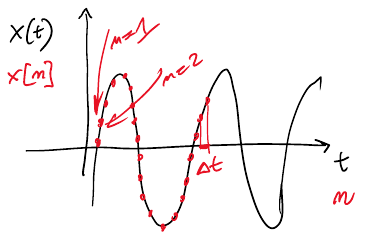
\includegraphics{immagini/lez1/segnaleTempoContinuo.jpg}
    \caption{Segnale a tempo continuo vs tempo discreto}
    \label{fig:tempoContinuo}
\end{figure}

Noi ci occuperemo di segnali monodirezionali, la variabile indipendente sara' 1, nel caso appena visto il tempo. Esistono anche segnali in cui ci sono piu' variabili indipendenti, l'immagine.

\begin{figure}[ht!]
    \centering
    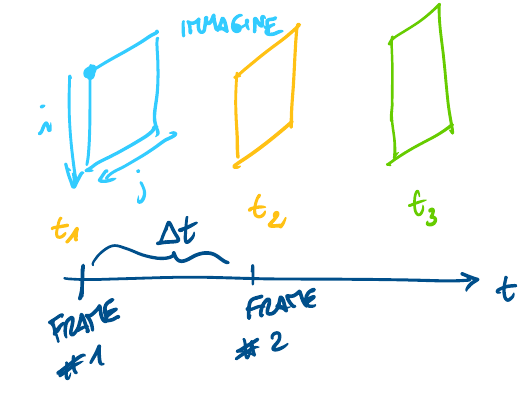
\includegraphics[scale=0.75]{immagini/lez1/segnaliMultidirezionali.jpg}
    \caption{Segnali multidirezionali}
    \label{fig:multidirezionali}
\end{figure}

Abbiamo un indice j che indica la riga ed un sensore i che indica la colonna, abbiamo due variabili indipendenti di tipo spaziale e se introduciamo un'altra variabile indipendente il tempo otteniamo una sequenza di immagini che e' un video: nel video abbiamo una variabile a tempo continuo che cresce (il tempo) che viene discretizzato in tutti i frame, e tra tutti i frame ci sara' un $\Delta t$. In questo caso abbiamo un segnale tridimensionale con 2 variabili indipendenti spaziali ed 1 variabile indipendente temporale.

\section{Sistema}
Cio' che manipola un segnale tipicamente si chiama sistema, che cos'e' un sistema?
Per adesso lo rappresentiamo come una scatola che e' il nostro algoritmo che ha in ingresso il nostro segnale tempo discreto x[n] ed in uscita ha un altro segnale tempo discreto y[n], cosa succede all'interno dell'algoritmo al momento non ci interessa, ma sappiamo che il segnale viene modificato, consideriamo che l'algoritmo sia una funzione y[n] = T{x[n]}.

\begin{figure}[ht!]
    \centering
    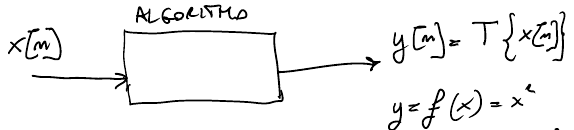
\includegraphics[scale=0.75]{immagini/lez1/sistema.jpg}
    \caption{Sistema}
    \label{fig:sistema}
\end{figure}

\section{Segnali e Sistemi}
Abbiamo i segnali che all'inizio saranno a tempo continuo, impareremo le caratteristiche di questi segnali ed impareremo a convertirli in tempo discreto con un convertitore analogico digitale, all'uscita di questo convertitore avremo un segnale a tempo discreto. Questo segnale tempo discreto impareremo a manipolarlo con un sistema che ci da un segnale in uscita che ancora una volta e' a tempo discreto. 
Per ora siamo ancora in un mondo a tempo discreto, pero' la nostra applicazione deve fare qualcosa nel mondo reale, allora in questo caso dobbiamo tornare nel tempo continuo, lo facciamo con un convertitore digitale analogico(DAC), quindi in uscita avremo un segnale a tempo continuo.

\begin{figure}[ht!]
    \centering
    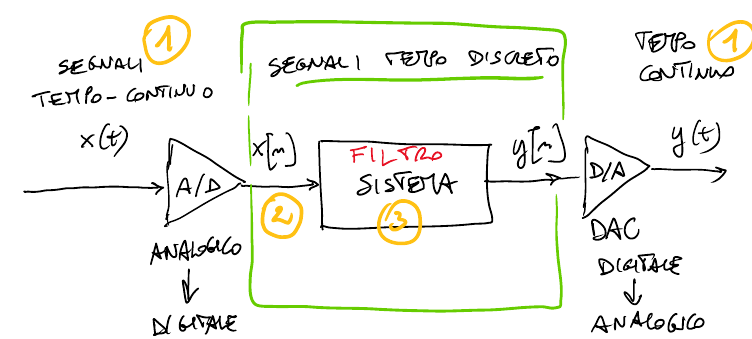
\includegraphics[scale=0.75]{immagini/lez1/continuoAdiscreto.jpg}
    \caption{Trasformare i segnali da tempo continuo a discreto}
    \label{fig:continuoAdiscreto}
\end{figure}

Dobbiamo partire dai segnali tempo continui perche' vogliamo capire che segnali digitali li caratterizzano, dopo di che parleremo dei segnali digitali, a questo punto potremo manipolare i segnali digitali parlando dei sistemi.
Infine torneremo ai segnali perche' vorremo essere in grado non solo di capire come funziona un sistema ma anche di progettarlo.
Un'altro modo di dire la parola sistema e' FILTRO, quindi dovremo essere in grado di scrivere degli algoritmi che siano dei filtri digitali che trasformino il segnale come vogliamo noi, lo faremo soprattutto nel contesto di Fourier.

\section{Segnale trigonometrico}
Nel contesto dei segnali tempo continui andiamo a ripassare un segnale trigonometrico, il piu' semplice e' il coseno:
\begin{equation}
    x(t) = A_0 \cos(2\pi f_0 t + \varphi_0)
\end{equation}

ricordiamo che t e' la variabile indipendente e non e' un parametro, certamente al variare di t cambia il segnale, ma siamo interessati al segnale nella sua interezza.

Andiamo ora a definire meglio tutti i parametri dell'equazione appena vista.

\subsection{Ampiezza}
 $A_0$ e' l'ampiezza del segnale, moltiplicare il coseno per un ampiezza significa aumentare o diminuire i punti massimi del coseno. Se $A_0 > 1 $ aumento i punti massini, altrimenti li diminuisco.

\subsection{Frequenza}
$f_0$ e' la frequenza del segnale cosinusoidale (in questo caso solo 1). Il concetto di frequenza e' un concetto base (con che frequenza mangi in una giornata), intendiamo il numero di volte che facciamo qualcosa in un unita' di tempo, per quanto ci riguarda la nostra unita' di tempo e' 1 secondo. Si misura in Heartz (hz) ed e' ottenuta dal numero di eventi fratto l'unita' di tempo. Nel nostro caso dato che stiamo parlando di un coseno, il quale e' periodico di periodo $2 k \pi$, questo sara' uguale a se stesso (si ripetera')dopo:

\begin{equation}
    2\pi f_0 t + \varphi_0 = 0 + 2 \pi k + \varphi
\end{equation}

dove k e' una costante e $k \in \mathbb(Z)$.
Da questa formula posso quindi scrivere che $t =\frac{k}{f_0} = k T_0$.
Dove $T_0 = \frac{1}{f_0}$ che e' il periodo del segnale.
Il segnale si ripetera' un'infinita' di volte, ma e' un modello.
Questo $f_0$ diremo indicativamente che e' grande per segnali ad alta frequenza, in questo caso se la frequenza e' grande il periodo (inverso della frequenza) sara' piccolo. Avremo anche segnali a bassa frequenza con $f_0$ piccolo ed il periodo grande. Queste stesse cose valgono anche per la lunghezza d'onda nelle radio.

\subsection{Pulsazione}
Un altra grandezza da considerare e' la pulsazione (frequenza angolare o velocita' angolare), generalmente detta $\omega_0$ ed e' banalmente uguale a $2\pi \cdot f_0$, cioe' portiamo in radianti la frequenza.
Si misura di conseguenza in radianti al secondo: $\frac{\mbox{RAD}}{1}$.
Soprattutto nel tempo discreto la velocita' angolare si usa molto, perche' viene riportata al concetto di frequenza.

\subsection{Fase}
$\varphi_0$ e' la fase, sposta il segnale a destra o sinistra rispettivamente se positiva o negativa. Ricordiamoci sempre che stiamo lavorando con segnali periodici, quindi potremo spostarli fino a $2\pi$, dopo di che tornano ad essere uguali, quindi generalizzando il concetto possiamo dire che tutto quello che esce dal range $0 \rightarrow 2\pi$ non modifica la funzione, una conseguenza di questa cosa e' che data una funzione periodica possiamo rimapparla togliendo $2\pi$.
In elaborazione dei segnali, per convenzione, si preferisce considerare il periodo base $-2\pi \rightarrow \pi$.

Nell'esempio vediamo come sommare o sottrarre una costante $\tau = 2$ trasla rispettivamente a destra e sinistra la funzione, esattamente il comportamento che ha la fase.

\begin{figure}[ht!]
    \centering
    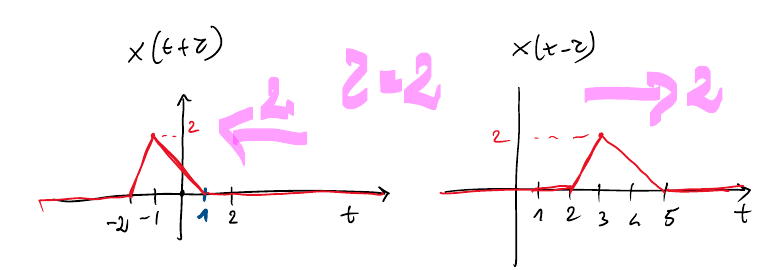
\includegraphics[scale=0.75]{immagini/lez1/modificareTempo.jpg}
\end{figure}



\chapter{Numeri complessi}
Facciamo un ripasso dei numeri complessi, perche' come vedremo saranno fondamentali per rappresentare i segnali che studieremo.

\section{Rappresentazione cartesiana}
La rappresentazione cartesiana di un numero complesso generale e':
\begin{equation}
    z = x + i y
\end{equation}
Dove $x  \in \mathbb R$, $x  \in \mathbb R$ ed $i = j = \sqrt{-1}$ ed e' detta unita' immaginaria.
Riportando queste informazioni su un piano cartesiano di cui l'asse delle Y appartiene ai numeri immaginari e l'asse delle X appartiene ai numeri reali otteniamo:

\begin{figure}[ht!]
    \centering
    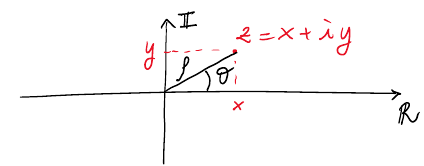
\includegraphics{immagini/lez2/rappCartesiana.jpg}
\end{figure}

\section{Rappresentazione Polare}
Oltre alla rappresentazione cartesiana esiste anche la rappresentazione polare, che punta a rappresentare il numero complesso utilizzando l'angolo che si forma tra l'asse x e la semiretta che rappresenta il numero complesso.

E la rappresentazione polare e':
\begin{equation}
    z = \rho [\cos \theta + i \sin \theta]
\end{equation}
Ci sono due componenti fondamentali in questa rappresentazione:
\begin{itemize}
    \item Modulo: $\rho$
    \item Fase: $\theta$
\end{itemize}

Si puo' passare tra le due rappresentazioni seguendo queste formule, ricordando che la rappresentazione cartesiana e': $z = x + iy$

\begin{table}[ht!]
    \centering
    \begin{tabular}{c|c}
        Rapp. Cartesiana & Rapp. Polare  \\
        \hline
        $x = \rho \cos \theta$ & $\rho = \sqrt{{x^2} + {y^2}}$\\
        $y = \rho \sin \theta$ & $\theta = \arctan \frac{y}{x}$\\
    \end{tabular}
    \caption{Passare da rappresentazione cartesiana a polare}
    \label{table:cambioRappresentazione}
\end{table}

\subsection{Esercizio}
Proviamo ora a fare un esercizio, dobbiamo rappresentare in forma polare il seguente numero immaginario espresso in forma cartesiana:
\begin{equation}
    z = -2 + i \cdot 3
\end{equation}

Cominciamo calcolando il modulo applicando semplicemente la formula vista in tabella \ref{table:cambioRappresentazione}:
\begin{equation}
    \rho = \sqrt{{-2^2} + {3^2}} = \sqrt{13}
\end{equation}

Successivamente calcoliamo la fase, sempre applicando la formula vista in tabella \ref{table:cambioRappresentazione}:
\begin{equation}
    \theta = \arctan - \frac{3}{2}
\end{equation}

Sulla fase abbiamo un problema, in quanto se dovessimo fare $\arctan - \frac{3}{2}$ alla calcolatrice ci risulterebbe $-56.3^{\circ}$, che non ha senso a prima vista in quanto negativo.
Spieghiamo questa cosa in quanto la calcolatrice ragiona solo nei quadranti 1 e 4 del piano cartesiano, quindi per sistemare questo problema dobbiamo sommare (o sottrarre) $180^{\circ}$ all'angolo che abbiamo trovato, ottenendo quindi: $123.7^{\circ}$.

\section{Coniugato Complesso}
Ogni numero immaginario ha un suo coniugato complesso, che ha lo stesso modulo e fase con segno invertito rispetto al numero immaginario di partenza.

\begin{equation}
    z = x + i y \rightarrow z^* = x - i y
\end{equation}

Graficamente otteniamo un punto ribaltato rispetto all'asse x:

\begin{figure}[ht!]
    \centering
    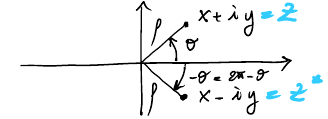
\includegraphics{immagini/lez2/coniugatoComplesso.jpg}
    \caption{Coniugato Complesso}
    \label{fig:coniugatoComplesso}
\end{figure}

\subsection{Operazioni}
Vediamo ora le operazioni con tra un numero immaginario ed il suo complesso.

Somma:
\begin{equation}
    z + z^* = x + x = 2x
\end{equation}
La somma di un numero complesso ed il suo coniugato e' uguale a due volte la sua parte reale.

Prodotto:
\begin{equation}
    z + z^* = (x + i y) \cdot (x - i y) = x^2 - i y x + i y x - i^2 y^2 = x^2 + y^2 = \rho^2
\end{equation}
Notiamo che $i^2 = (\sqrt{-1})^2 = -1$.

\section{Teorema fondamentale dell'algebra}
Data un equazione polinomiale di grado $N \ge 1$
\begin{equation}
    a_n z^n + a_{n-1} z ^ {n-1} + \mbox{...} a_1 z + a_0 = 0
\end{equation}
Ammette sempre e solo N soluzioni (radici) in $\mathbb C$.
Inoltre se $a_k \in \mathbb R$ (sono numeri reali) le soluzioni sono reali o complesse coniugate. Questa cosa introduce una simmetria, sappiamo che se i termini del polinomio sono reali non avremo mai un complesso da solo ma sara' sempre accompagnato dal suo coniugato ed e' una cosa che servira' successivamente.

\section{Formula di Eulero}
Esprimo prima cos, sin e l'esponenziale in serie:
\begin{equation}\begin{split}
    \cos& \theta = 1 - \frac{1}{2!} \theta^2 + \frac{1}{4!} \theta^4 - \frac{1}{6!} \theta^6 \mbox{...} \\
    \sin& \theta = \theta - \frac{1}{3!} \theta^3 + \frac{1}{5!} \theta^5 - \frac{1}{7!} \theta^7 \mbox{...} \\
    e^{\theta}& = 1 + \theta + \frac{\theta^2}{2!} + \frac{\theta^3}{3!} + \frac{\theta^4}{4!} + \mbox{...}
\end{split}\end{equation}

Eulero nota che se cerchiamo di calcolare l'esponenziale in serie moltiplicando l'esponente per i, il fattore i e' presente solo nei termini dispari, se sviluppiamo le potenze. 

\begin{equation}\begin{split}
    e^{i \theta}& = 1 + (i \theta) + \frac{(i \theta)^2}{2!} + \frac{(i \theta)^3}{3!} + \frac{(i \theta)^4}{4!} + \mbox{...} \\
    & = 1 + i \theta - \frac{\theta^2}{2!} - \frac{i \theta^3}{3!} + \frac{\theta^4}{4!} + \mbox{...}
\end{split}\end{equation}

Da questa considerazione troviamo la formula di Eulero :
\begin{equation}
    e^{i \theta} = \cos \theta + i \sin \theta
\end{equation}

\begin{figure}[ht!]
    \centering
    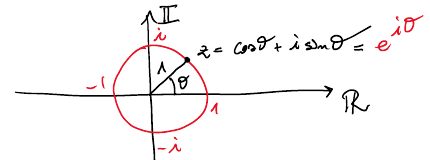
\includegraphics{immagini/lez2/formulaEulero.jpg}
    \caption{Rappresentazione su cerchio unitario}
    \label{fig:euleroGrafico}
\end{figure}

\subsection{Formule di Eulero inverse}
Esistono delle formule di Eulero con cui trovare sin e cos a partire dall'esponenziale:

\begin{equation}\begin{split}
    \cos \theta & = \frac{e^{i \theta} + e^{-i \theta}}{2}\\
    \sin \theta & = \frac{e^{i \theta} - e^{-i \theta}}{2i}
\end{split}\end{equation}

\chapter{Spazi vettoriali}
Dagli spazi vettoriali dall'algebra lineare agli spazi vettoriali in cui le basi sono funzioni (spazi di Hilbert).
Per fare questo passaggio ripassiamo i vettori.

\section{Rappresentazione}
Esistono due tipi di rappresentazione, cartesiana e polare.

\begin{figure}[ht!]
    \centering
    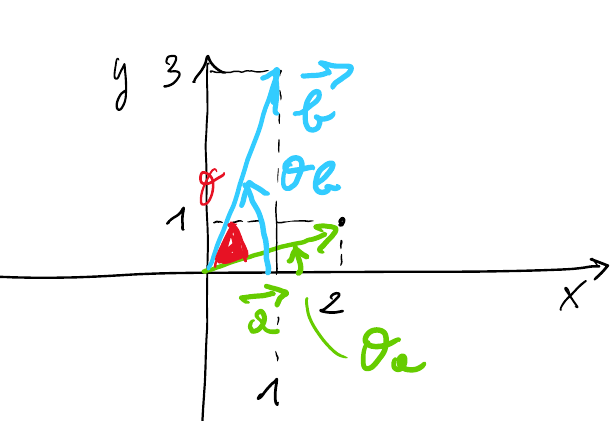
\includegraphics[scale=0.35]{immagini/lez7/vettori.jpg}
\end{figure}

\[\begin{split}
    \Vec{a} =
    \begin{pmatrix}
    2\\
    1
    \end{pmatrix}
    \mbox{  }|\Vec{a}| &= \sqrt{1+4} = \sqrt{5} \\
    \Theta_a &= arctan \frac{1}{2} \\
    \Vec{b} =
    \begin{pmatrix}
    1\\
    3
    \end{pmatrix}
    \mbox{  }|\Vec{b}| &= \sqrt{1+9} = \sqrt{10} \\
    \Theta_b &= arctan 3
\end{split}
\]

\section{Prodotto Scalare}
Il prodotto scalare di due vettori e' la loro combinazione lineare (il primo elemento del primo vettore moltiplicato per il primo elemento del secondo vettore, e cosi' via). Il risultato e' un numero ed il simbolo e' $\langle\Vec{a}, \Vec{b}\rangle$ o $\Vec{a} \cdot \Vec{b}$.

\begin{figure}[ht!]
    \centering
    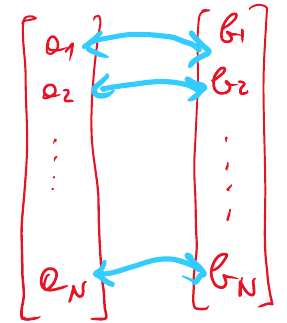
\includegraphics[scale=0.35]{immagini/lez7/prodottoScalare.jpg}
\end{figure}

Rappresentazione cartesiana:
\[\begin{split}
    [2, 1] [1, 3] = 2 \cdot 1 + 1 \cdot 3 = 5
\end{split}\]

\section{Vettori ortogonali}
Due vettori sono ortogonali quando il loro prodotto scalare e' zero.

\begin{figure}[ht!]
    \centering
    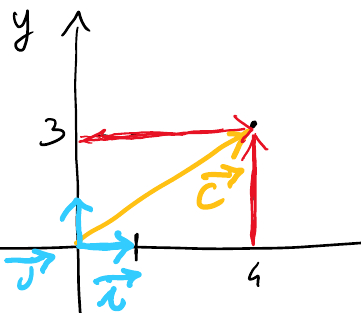
\includegraphics[scale=0.35]{immagini/lez7/vettoriOrtogonali.jpg}
\end{figure}

i e j sono detti VERSORI, posso riscrivere il vettore C come combinazione dei versori:

\[
    \Vec{C} = \Vec{i} 4 + \Vec{j} \cdot 3 
\]

Di conseguenza possiamo considerare C come combinazione lineare delle basi nello spazio vettoriale e il modulo del vettore e' la sua proiezione ortogonale.
Quindi riconducendo questo discorso ai segnali, ogni volta che analizziamo un vettore ne facciamo il prodotto scalare dal prodotto scalare per fare una "sintesi" del vettore rimetto insieme i prodotti scalari.

\chapter{Segnali a tempo continuo}
Dopo aver ripassato i numeri complessi torniamo a parlare di segnali.
\section{Terminologia}
Innanzitutto diamo prima della terminologia che ci servira' per tutta la durata del corso, in quanto valgono sia per segnali tempo-continui sia per i tempo-discreti:
\begin{itemize}
    \item SINTESI DI UN SEGNALE: composizione di segnali (solitamente) "semplici" per ottenere un segnale piu' "complesso"
    \item ANALISI DI UN SEGNALE: decomposizione di un segnale "complesso" in un insieme di segnali piu' "semplici"
\end{itemize}

Per aiutarci usiamo una formula, usando segnali a tempo continui, abbiamo un segnale tempo continuo e lo scomponiamo in composizione di somma di segnali piu' semplici ($a_k$)
\begin{equation}
    x(t) = \sum_{k = -L}^{U} a_k s(t, \xi _k)
\end{equation}

Analizzando questa espressione diciamo che il passaggio da $x(t)$ alla sommatoria e' l'operazione di analisi il cui risultato e' la combinazione lineare di $a_k, \xi_k$
Viceversa il passaggio dalla sommatoria alla funzione $x(t)$ e' l'operazione di sintesi, il cui risultato ovviamente e' $x(t)$.
La notazione $s(t, \xi_k)$ e' il segnale "semplice" o base e vediamo che non solo dipende dal tempo ma anche da un set di parametri, in questo caso chiamati $\xi_k$: $\xi_k = {f_k; \varphi_k}$, questi parametri ci permettono di comporre segnali diversi. Ad esempio il set di parametri per come abbiamo visto fino ad ora per il seno sono ampiezza, fase e frequenza.

\section{Sintesi di segnali co-sinusoidali}
Possiamo combinare linearmente segnali sinusoidali per avere segnali piu' articolati/realistici.
Vediamo un esempio:
\begin{equation}
    s(t, k) = \cos (2\pi f_k t + \varphi_k)
\end{equation}

\begin{equation}\begin{split}
    x(t) &= \frac{419}{1713} \cos (2\pi 200 t + \frac{1693}{3527} \pi) \\
    &+ \frac{629}{1069} \cos (2\pi 400 t + \frac{236}{395} \pi) \\
    &+ \frac{421}{431} \cos (2\pi 500 t - \frac{34}{917} \pi) \\
    &+ \frac{76}{279} \cos (2\pi 1600 t - \frac{232}{503} \pi) \\
    &+ \frac{89}{942} \cos (2\pi 1700 t )
\end{split}\end{equation}
Dall'esempio abbiamo tanti segnali sinusoidali che sommati danno come risultato un segnale piu'"complicato" che simula la lettere o in inglese.
Abbiamo una costante (Ampiezza) che moltiplica il coseno e dentro al coseno abbiamo una costante (frequenza) che moltiplica il tempo (t) + la fase (sempre una costante).

Quindi la sintesi ci permette di avere un segnale complicato, e sono oggettivamente simili a dei segnali reali.

Se disegniamo (tramite MatLab) il segnale risultante, otteniamo:

\begin{figure}[ht!]
    \centering
    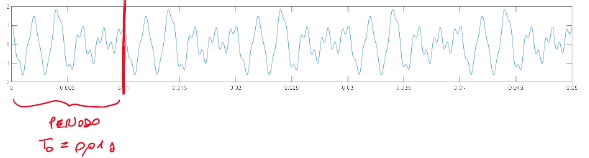
\includegraphics[scale=0.75]{immagini/lez2/esempioSintesiSegnali.jpg}
    \caption{Esempio di sintesi di segnali}
    \label{fig:esSintesiSegnali}
\end{figure}

l'unica osservazione che possiamo fare guardando il grafico e' che il periodo e' $T_0=0,01s$ ed e' quindi un segnale periodico.
Le fasi ci dicono solo come abbiamo traslato i segnali tra di loro per ottenere questa forma.

Andiamo a mettere insieme l'uso dei numeri complessi che abbiamo visto con il segnale in esempio, nonostante non ci sia nessun numero complesso c'e' il coseno e quindi possiamo usare la formula di Eulero inverso per scrivere il segnale in modo piu' compatto.
Abbiamo fatto inizialmente una sintesi:
\begin{equation}
    x(t) = \sum_{k = 1}^{5} A_k \cos (2\pi f_k t + \varphi_k)
\end{equation}

Tutti i valori con k sono dei numeri. 
Prendiamo uno degli elementi di prima, che posso scrivere con la formula di Eulero inversa del coseno.
$\theta$ e' tutto quello che c'e' nelle parentesi del coseno.

\begin{equation}
    A_k \cos (2\pi f_k t + \varphi_k) = \frac{A_k}{2} {e^{i(2\pi f_k t + \varphi_k)} + e^{-i(2\pi f_k t + \varphi_k)} }
\end{equation}

Se io adesso faccio un cambio di notazione:
\begin{equation}\begin{split}
    &\frac{A_k}{2} = a_k \\
    &f-k = -f_k
\end{split}\end{equation}

Riscriviamo quindi il nostro pezzo di segnale con la nuova notazione:
\begin{equation}
    = a_k e ^{i 2\pi f_k t} e^{i \varphi_k} + a_k e ^{-i 2\pi f_k t} e^{-i \varphi_k}
\end{equation}

Notiamo che:
\begin{equation}\begin{split}
    &a_k e^{i \varphi_k} = b_k \\
    &a_k e^{-i \varphi_k} = b_k^{\circ}
\end{split}\end{equation}

Sono uno un numero complesso e l'altro il suo coniugato, perche' il modulo ($a_k$) e' uguale per tutti e due mentre la fase cambia di segno.
Posso anche notare che c'e' un $-f_k$ che trasformo in $f-k$.
In forma compatta quindi posso dire che il segnale e':
\begin{equation}
    b_k e^{i 2\pi f_k t} + b_k^{*} e^{i 2\pi f_k t}
\end{equation}
Estendo ulteriormente la notazione e chiamo $b-k = b_k^{*}$. Tutto questo perche' voglio scrivere questo come due pezzi di un indice.

Riassumendo ho scritto:
\begin{equation}\begin{split}
    x(t) &= \sum_{k = 1}^{5} A_k \cos (2\pi f_k t + \varphi_k) \\
    &= \sum_{k = -5, k \neq 0}^{5} b_k e{i 2 \pi f_k t}
\end{split}\end{equation}

Questo passaggio lo possiamo fare se:
\begin{equation}\begin{split}
    &b-k = b_k^* \\
    &\frac{A_k}{2} e^{i \varphi_k} = b_k \\
    &-f_k = f-k
\end{split}\end{equation}

La seconda quantita' ($b_k$) e' il FASORE, ed e' solo un numero complesso in rappresentazione polare, perche' si risalta la fase.

\section{Spettro del segnale}
Lo spettro del segnale e' una rappresentazione del segnale basato sull'enumerazione di frequenza e fasore.

Vediamo come e' rappresentato un segnale:
\begin{equation}
    \{ (f_{-n}; n_{-n})(f_{-n+1}; b_{-n+1}) \mbox{...} (f_0; b_0); (f_1, b_1) \mbox{...} (f_n, b_n) \}
\end{equation}

Se usiamo la rappresentazione vista prima possiamo riscrivere la funzione come N frequenze, N fasori e tutti i coniugati complessi piu' l'elemento zero:
\begin{equation}
    \{ (-f_n; b_n^*)(-f_{n+1}; b^*_{-n+1}) \mbox{...} (0; b_0); (f_1, b_1) \mbox{...} (f_n, b_n) \}
\end{equation}

Lo spettro e' l'input che diamo per sintetizzare il segnale, e' quindi utile modificare e fare delle operazioni sullo spettro perche' modificando lo spettro viene modificato il segnale che andiamo a sintetizzare.

\subsubsection{Esempio}
Abbiamo 3 modi per rappresentare lo spettro:
\begin{itemize}
    \item Elencando i segnali che lo compongono per enumerazione
    \item Graficamente costruendo due grafici:
    \begin{itemize}
        \item Uno per il modulo 
        \item Uno per la fase
    \end{itemize}
    \item Graficamente costruendo due grafici:
    \begin{itemize}
        \item Uno per la parte reale
        \item Uno per la parte immaginaria
    \end{itemize}
\end{itemize}

Vediamo un esempio, inizialmente abbiamo un segnale rappresentato come sommatoria (un segnale sintetizzato):
\begin{equation}
    \sum_{k = -2}^{2} b_k e^{i 2 \pi f_k t}
\end{equation}

Andiamo ora ad elencare tutti i valori che $b_k$ (sono valori che ci ha dato lui), non c'e' bisogno di farlo per i negativi, perche' saranno gli opposi, o i complessi coniugati per le fasi:

\begin{equation}\begin{split}
   k=2 &\rightarrow 3 e^{i \frac{\pi}{2}} \\
   k=1 &\rightarrow \frac{1}{2} e^{-i \frac{\pi}{3}} \\
   k=0 &\rightarrow 4 \\
\end{split}\end{equation}

Ora facciamo la stessa cosa per i valori di $f_k$:

\begin{equation}\begin{split}
   k=2 &\rightarrow 250 \mbox{Hz} \\
   k=2 &\rightarrow 30 \mbox{Hz} \\
   k=2 &\rightarrow 0 \mbox{Hz} \\
\end{split}\end{equation}

Ora ricaviamo lo spettro di questo segnale scrivendolo inizialmente per enumerazione, accoppiando le frequenze ed i loro fasori, notando che dobbiamo accoppiare le frequenze negative con i fasori coniugati di quelli che abbiamo ricavato precedentemente:
\begin{equation}
    \{ (-250 \mbox{Hz}; 3e^{-i\frac{\pi}{2}}); (-30 \mbox{Hz}; \frac{1}{2}e^{i\frac{\pi}{3}}); (0 \mbox{Hz}; 4); (250 \mbox{Hz}; 3e^{i\frac{\pi}{2}}); (30 \mbox{Hz}; \frac{1}{2}e^{-i\frac{\pi}{3}}) \}
\end{equation}

Da questa rappresentazione enumerativa ricaviamo la prima rappresentazione grafica, in un grafico mettiamo tutti i moduli, mentre nel secondo grafico rappresentiamo le fasi.
Sull'asse delle x abbiamo tutte le frequenze, mentre sull'asse verticale nel caso del primo grafico rappresentiamo il numero che moltiplica il fasore (il modulo nella rappresentazione polare dei numeri complessi), mentre nel secondo grafico sull'asse delle x abbiamo sempre le frequenze, mentre sull'asse delle y abbiamo la fase (ovvero il numero che moltiplica i):

\begin{figure}[ht!]
    \centering
    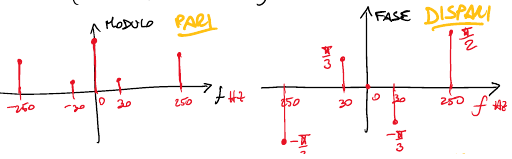
\includegraphics{immagini/lez3/moduloFase.jpg}
\end{figure}

Notiamo in questa rappresentazione che ci sono delle simmetrie:
\begin{itemize}
    \item Il modulo e' una funzione pari: ovvero che e' simmetrica rispetto all'asse y
    \item la fase e' una funzione dispari: ovvero che e' simmetrica rispetto all'origine degli assi
\end{itemize}

Esiste anche una rappresentazione in cui in un grafico rappresentiamo la parte reale mentre nell'altro la parte immaginaria. 
Come prima sull'asse x abbiamo le frequenze, mentre per mettere i punti sull'asse delle y devo prima trasformare i numeri complessi nella loro forma cartesiana, utilizzando la formula di Eulero. Ancora una volta troviamo solo i positivi e poi per i negativi semplicemente invertiamo il segno:

\begin{equation}\begin{split}
    &3e ^{i\frac{\pi}{2}} = 3(\cos \frac{\pi}{2} + i \sin \frac{\pi}{2}) = 3i \\
    &\frac{1}{2} e ^{-i\frac{\pi}{3}} = \frac{1}{2}[\cos(-\frac{\pi}{3}) + i \sin(\frac{-\pi}{3})] = \frac{1}{4} -i\frac{\sqrt{3}}{4}
\end{split}\end{equation}

\begin{figure}[ht!]
    \centering
    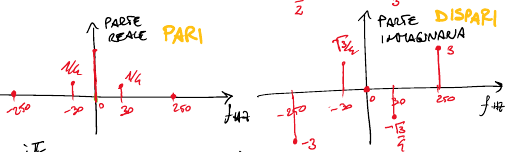
\includegraphics{immagini/lez3/realeImmaginaria.jpg}
\end{figure}

\subsection{Proprieta' dello spettro}
Vediamo come e' possibile manipolare un segnale attraverso la manipolazione dello spettro, utilizzando delle proprieta' dello spettro.

\subsubsection{Moltiplicazione per una costante}

\begin{equation}
  \textcolor{red}{C} x(t) =  \sum_{k = -n}^{n} \textcolor{red}{C}b_k e^{i 2 \pi f_k t}
\end{equation}

Quando moltiplico un segnale per una costante \textcolor{red}{C} lo spettro rimane uguale ma i fasori vengono moltiplicati per la costante stessa.

Spettro:
\begin{equation}
    \{ (-f_n; \textcolor{red}{C}b_n^*)(-f_{n+1}; \textcolor{red}{C}b^*_{-n+1}) \mbox{...} (0; \textcolor{red}{C}b_0); (f_1, \textcolor{red}{C}b_1) \mbox{...} (f_n, \textcolor{red}{C}b_n) \}
\end{equation}

\subsubsection{Somma di una costante}
QUando moltiplico un segnale per una costante \textcolor{red}{C}, lo spettro rimane uguale con l'unica differenza che il fasore dell'elemento 0 viene sommato alla costante \textcolor{red}{C}.

\begin{equation}
   x(t) + \textcolor{red}{C} =  \sum_{k = -n}^{n} b_k e^{i 2 \pi f_k t} + \textcolor{red}{C} e^{i 0}
\end{equation}

\begin{equation}
    \{ (-f_n; b_n^*)(-f_{n+1}; b^*_{-n+1}) \mbox{...} (0; b_0 + \textcolor{red}{C}); (f_1, b_1) \mbox{...} (f_n, b_n) \}
\end{equation}

\subsubsection{Somma di due segnali}
Sommare due segnali (con frequenze diverse) significa combinare i due segnali, ovvero prendere tutte le coppie (da entrambi i segnali) che hanno frequenze diverse, nel caso in cui ci sono frequenze uguali dei due segnali, si sommano i fasori di quelle frequenze.

\begin{equation}\begin{split}
    &x(t) = \{ (-f_n; b_n^*)(-f_{n+1}; b^*_{-n+1}) \mbox{...} (0; b_0); (f_1, b_1) \mbox{...} (f_n, b_n) \} \\
    &y(t) = \{ (-g_n; d_n^*)(-g_{n+1}; d^*_{-n+1}) \mbox{...} (0; d_0); (g_1, d_1) \mbox{...} (g_n, b_n) \} \\
\end{split}\end{equation}

Facciamo un esempio, consideriamo come $x(t)$ il segnale con lo spettro di prima, mentre definiamo lo spettro di $y(t)$ per enumerazione:

\begin{equation}
    \{ (-125 \mbox{Hz}; 2e^{i\frac{\pi}{2}}); (-30 \mbox{Hz}; \frac{2}{3}e^{i\frac{\pi}{4}}); (125 \mbox{Hz}; 2e^{-i\frac{\pi}{2}}); (30 \mbox{Hz}; \frac{2}{3}e^{-i\frac{\pi}{4}}) \}
\end{equation}

Applichiamo quello detto prima e facciamo la composizione dei due spettri:

\begin{equation}\begin{split}
    S_{\textcolor{red}{x + y}} =  &\{ (-250 \mbox{Hz}; 3e^{-i\frac{\pi}{2}}); (-125 \mbox{Hz}; 2e^{i\frac{\pi}{2}}); (-30 \mbox{Hz}; \frac{2}{3}e^{i\frac{\pi}{4}} + \frac{1}{2}e^{i\frac{\pi}{3}}); (0 \mbox{Hz}; 4); \\
     &(250 \mbox{Hz}; 3e^{i\frac{\pi}{2}}); (125 \mbox{Hz}; 2e^{-i\frac{\pi}{2}}); (30 \mbox{Hz}; \frac{2}{3}e^{-i\frac{\pi}{4}} + \frac{1}{2}e^{-i\frac{\pi}{3}}) \}
\end{split}\end{equation}


\subsubsection{Traslazione nel tempo}
Traslare nel tempo una funzione co-sinusoidale, come gia' abbiamo visto, significa sommare o sottrarre l'argomento della funzione per una costante $\tau$. 
Quello che succede e' che lo spettro rimane uguale, ma i fasori vengono moltiplicati, per un cosiddetto "termine di fase" che dipende dalla frequenze e non dal tempo.  Quindi cambia la fase del numero complesso ma non cambia il modulo.

Quello che ci stiamo chiedendo e' cosa succede in questo caso:
\begin{equation}\begin{split}
    &x(t) \leftrightarrow S_x \\
    &y(t) = x(t - \textcolor{red}{\tau}) \leftrightarrow S_y \mbox{?}
\end{split}\end{equation}

Cominciamo calcolando $y(t)$ esplicitamente:
\begin{equation}\begin{split}
     y(t) &=  \sum_{k = -n}^{n} b_k e^{i 2 \pi f_k (t - \textcolor{red}{\tau})} \\
\end{split}\end{equation}

Da cui otteniamo lo spettro:

\begin{equation}
    \{ (-f_n; b_n^* e^{i 2 \pi f_k  \textcolor{red}{\tau}}) \mbox{...} (0; b_0 \cdot 1); \mbox{...} (f_n, b_n e^{i 2 \pi f_k \textcolor{red}{\tau}}) \}
\end{equation}

\subsubsection{Moltiplicazione per un esponenziale complesso}
Moltiplicare un segnale per un esponenziale complesso significa trasformare il segnale in un numero costante che dipende dal tempo ma non e' un segnale reale. Quello che succede e' che le frequenze vengono spostate (sommate o sottratte) del numero. 
Notiamo che e' l'unica proprieta' che modifica le frequenze.

Ricordiamo che:
\begin{itemize}
    \item Se moltiplichiamo per un numero negativo il segnale verra' spostato verso destra
    \item Se moltiplichiamo per un numero positivo il segnale verra' spostato verso sinistra
\end{itemize}

\begin{equation}\begin{split}
     y(t) &=  \sum_{k = -n}^{n} b_k e^{i 2 \pi f_k t} e^{i 2 \pi \Tilde{f} t}\\
     &= \sum_{k = -n}^{n} b_k e^{i 2 \pi (f_k = \Tilde{f}) t}
\end{split}\end{equation}

Da cui otteniamo lo spettro per enumerazione:
\begin{equation}
    \{ (-f_n \textcolor{red}{+ \Tilde{f}}; b_n^*)(-f_{n+1} \textcolor{red}{+ \Tilde{f}}; b^*_{-n+1}) \mbox{...} (0 \textcolor{red}{+ \Tilde{f}}; b_0); (f_1 \textcolor{red}{+ \Tilde{f}}, b_1) \mbox{...} (f_n \textcolor{red}{+ \Tilde{f}}, b_n) \}
\end{equation}

Vediamo come ulteriore prova del fatto che moltiplicando per un esponenziale complesso si ottiene un segnale non reale il fatto che se tracciamo i garfici di modulo e frequenza questi non sono piu' simmetrici:

\begin{figure}
    \centering
    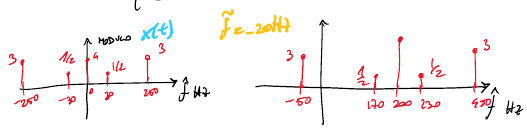
\includegraphics{immagini/lez3/molitplicazioneEsponenzialeComplesso.jpg}
\end{figure}

\section{Modulazione di ampiezza}
La modalita' di trasmissione di un segnale in modulazione d'ampiezza e' quella utilizzata dalle radio AM, che trasmettono in modulazione di ampiezza per poter aumentare di molto le frequenze di trasmissione, cosi' facendo i segnali evitano disturbi di frequenze.

Vediamo come "modulare" un segnale, immaginiamo che il segnale che vogliamo trasmettere sia x(t) e questo che viene trasmesso e' x(t) che e' l'AMPIEZZA, mentre il coseno e' la portante e $\Tilde{f}$ e' la frequenza a cui dobbiamo sintonizzarci per ascoltare i segnale:

\begin{equation}
    y(t) = x(t) \cos (2\pi \Tilde{f} t)
\end{equation}

Che spettro avra' il segnale trasmesso? per farlo utilizziamo le proprieta' che abbiamo appena visto, otteniamo questa cosa applicando il teorema di Eulero inverso del coseno:

\begin{equation}
    y(t) = x(t) \{ \frac{e}{2}^{i 2 \pi \Tilde{f} t} + \frac{e}{2}^{-i 2 \pi \Tilde{f} t}  \}
\end{equation}

Vediamo che in questa equazione abbiamo delle proprieta' che abbiamo appena visto:
\begin{itemize}
    \item La proprieta' di somma di una costante C, in questo caso $C = \frac{1}{2}$
    \item La proprieta' di somma di due segnali, perche' appunto i due esponenziali si sommano
    \item La proprieta' di moltiplicazione per un esponenziale complesso, che e' $\Tilde{f}$ 
\end{itemize}

Lo spettro finale sara' quindi dato dall'unione di tutti i segnali dei due insiemi spostato di $\Tilde{f}$ e moltiplicato per $\frac{1}{2}$ (ovvero tutti i fasori saranno moltiplicati per $\frac{1}{2}$).

E se tracciamo i grafici di modulo e frequenza vediamo che viene modificata la frequenza e quindi l'ampiezza del segnale.
Nel nostro caso consideriamo $\Tilde{f} = 1000 \mbox{Hz}$ e notiamo che il tutti i punti del grafico vengono traslati di 1000 posizioni.

\begin{figure}[ht!]
    \centering
    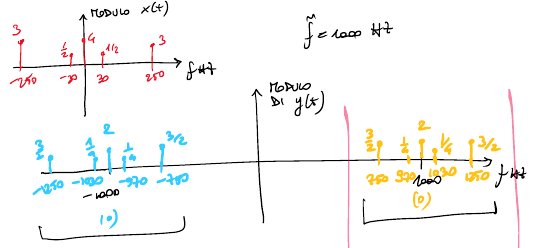
\includegraphics{immagini/lez3/modulazioneAmpiezza.jpg}
\end{figure}

\section{Esercizio di sintesi}
Dato il seguente spettro:

\begin{equation}
    \{ (-3 \mbox{Hz}; 1 + i\sqrt{3}),(-2 \mbox{Hz}; \frac{\sqrt{3}}{2} - i \frac{1}{2}),(0 \mbox{Hz}; 3),(2 \mbox{Hz}; \frac{\sqrt{3}}{2}  i \frac{1}{2}),(3 \mbox{Hz}; 1 + i\sqrt{3}) \}
\end{equation}

Calcoliamo qual'e' il segnale $x(t)$ a cui appartiene.
Innanzitutto notiamo che il segnale e' un segnale reale, in quanto tutti i segnali che lo compongono sono a coppie ed i fasori sono complessi coniugati tra di loro, ed inoltre sono in forma cartesiana, quindi li trasformiamo in forma polare:

\begin{equation}\begin{split}
    &z = 1 \pm i \sqrt{3}: \\
    &\rho = \sqrt{i^2 + \sqrt{3}^2} = 2 \\
    &\theta = arctan \frac{\pm \sqrt{3}}{1} = \pm \frac{\pi}{3}\\
    &z = 2 e^{\pm i \frac{\pi}{3}}
\end{split}\end{equation}

\begin{equation}\begin{split}
    &z = : \frac{\sqrt{3}}{2} \pm i \frac{1}{2}\\
    &\rho = \sqrt{(\frac{\sqrt{3}}{2})^2 + (\pm i \frac{1}{2})^2} = 1 \\
    &\theta = arctan \frac{\pm \frac{1}{2}}{\frac{\sqrt{3}}{2}} = arctan \frac{1}{\sqrt{3}} = \pm \frac{\pi}{6} \\
    &z = 1 e^{\pm i \frac{\pi}{6}}
\end{split}\end{equation}

Ora semplicemente copiamo ed incolliamo le frequenze ed i fasori, secondo la formula che abbiamo visto prima:

\[\begin{split}
    x(t) &=\{ (-3 \mbox{Hz}; 2e^{i \frac{\pi}{3}} \cdot e^{-i2 \pi 3 t}) + (-2 \mbox{Hz}; e^{-i \frac{\pi}{6}} \cdot e^{-i2 \pi 2 t}) + (0 \mbox{Hz}; 3e^{i 0} \cdot e^{-i2 \pi 0 t}) \\
    &+ (2 \mbox{Hz}; e^{i \frac{\pi}{6}} \cdot e^{-i2 \pi 2 t}) + (3 \mbox{Hz}; 2e^{-i \frac{\pi}{3}} \cdot e^{-i2 \pi 3 t}) \}
\end{split}\]

A questo punto mettiamo insieme gli esponenti degli esponenziali moltiplicati tra di loro, inoltre raccogliamo la i e portiamo fuori i meno in modo tale che gli esponenziali con la stessa base siano complessi coniugati per poter applicare la formula di Eulero:

\[\begin{split}
    2e^{-i(2\pi 3t - \frac{\pi}{3}} + e^{-i(2\pi 2t + \frac{\pi}{3}} + 3 + e^{i(2\pi 2t + \frac{\pi}{6}} + 2e^{i(2\pi 3t - \frac{\pi}{3}}
\end{split}\]

Applichiamo la formula di Eulero tra i coniugati ed ottieniamo:

\[
    4 \cos{(2\pi 3t - \frac{\pi}{3})} + 2 \cos{(2\pi 2t +\frac{\pi}{6})} + 3
\]

Ora dobbiamo trovare qual'e' lo spettro del segnale $y(t) = x(t - 10)$ e va derivato dallo spettro di $x(t)$. Sappiamo che si tratta di una traslazione nel tempo, quindi semplicemente applichiamo la regola vista in precedenza della traslazione nel tempo. Ricordando che vanno moltiplicati i fasori per la costante.
Quello che facciamo e' prendere lo spettro che precedentementa avevamo modificato portando le fasi in rappresentazione polare e moltiplichiamo la costante ai fasori:

\[\begin{split}
    x(t) &=\{ (-3 \mbox{Hz}; 2e^{i \frac{\pi}{3}} \cdot e^{-i2 \pi 3 \textcolor{red}{10}}) + (-2 \mbox{Hz}; e^{-i \frac{\pi}{6}} \cdot e^{-i2 \pi 2 \textcolor{red}{10}}) + (0 \mbox{Hz}; 3e^{i 0} \cdot e^{-i2 \pi 0 \textcolor{red}{10}}) \\
    &+ (2 \mbox{Hz}; e^{i \frac{\pi}{6}} \cdot e^{-i2 \pi 2 \textcolor{red}{10}}) + (3 \mbox{Hz}; 2e^{-i \frac{\pi}{3}} \cdot e^{-i2 \pi 3 \textcolor{red}{10}}) \}
\end{split}\]
%non l'ho finito perche' non mi sembra sensato copiare gli esercizi, li terro' sul quaderno

\section{Terminologia}
Diamo delle definizioni in modo da avere un base terminologica:
\begin{itemize}
    \item Frequenze armoniche: sono tutti i multipli interi di una frequenza detta frequenza fondamentale $F_0$.
\end{itemize}

Se ad esempio la frequenza base $F_0 = 10$ Hz, la $3^a$ armonica sarebbe 30 Hz e cosi' via.

\section{Teorema della serie di Fourier}
Cominciamo notando che partendo da una frequenza $F_0$ nota, moltiplicandola per una costante $k \in \mathbf{R}$ crescente, il periodo $T_0$ del segnale diminuisce, in particolare $\cos{(s\pi k F_0 t)}$ avra' periodo $T= \frac{1}{k \cdot T_0} = \frac{1}{k} T_0$.
Questa cosa ci fa capire che se uso frequenze armoniche di $F_0$ sicuramente sono periodiche anche per il periodo base $T_0$. Di conseguenza se faccio la sintesi tra frequenze armoniche sicuramente so che il segnale risultante sia periodico:
\begin{equation}
    \mbox{Se } f_k = k F_0 \Leftrightarrow x(t) = \sum_{k} b_k e^{i 2 \pi f_k t} \mbox{PERIODICO}
\end{equation}

Il viceversa, ovvero che se scindo un segnale periodico posso scriverlo come combinazione di infinite frequenze armoniche si chiama teorema sulle serie di Fourier:
$x(t)$ e' un segnale (TEMPO CONTINUO) periodico di periodo $T_0$ puo' essere sintetizzato come:
\begin{equation}
    \mbox{SINTESI: }x(t) = \sum_{k = - \infty}^{+ \infty} a_k e^{\textcolor{red}{+} j 2\pi F_0 k t} \rightarrow F_0 = \frac{1}{T_0}
\end{equation}

dove

\begin{equation}
    \mbox{ANALISI: } a_k = \frac{1}{T_0} \int_0^{T_0} x(t) e^{\textcolor{red}{-} j 2\pi F_0 k t} dt
\end{equation}

Ricordiamoci che se la sintesi deve dare un segnale reale ogni $a_k$ deve avere un suo complesso coniugato ed in particolare $a_k^* = a-k$.

Inoltre che il segnale $a_0$ sara' dato da $\frac{1}{T_0} \int_0^{T_0} x(t) \cdot 1 dt$, ovvero l'integrale del segnale nel periodo.

\subsection{Spettro di un segnale periodico}
Come ci aspettiamo lo spettro di un segnale periodico avra' infinite componenti.

\subsection{Esempio}
Facciamo l'analisi di un segnale periodico $x(t) = |\sin{\frac{2\pi t}{T_s}}|$.
Quello che faremo nella pratica e' rettificare un segnale sinusoidale.

Iniziamo disegnando il grafico, notiamo subito che essendo il modulo di un seno, sara' il grafico del seno con le parti negative ribaltate rispetto all'asse x.

Il seno sara' uguale a 0 quando $\frac{2\pi t}{T_s} = k\pi$ (ovvero quando l'argomento del seno e' $k \pi$), cancellando il $\pi$ ottengo che in tutti i punti $t = \frac{k T_s}{2}$, sono tutti i punti in cui il seno inteseca l'asse orizzontale.

\begin{figure}[ht!]
    \centering
    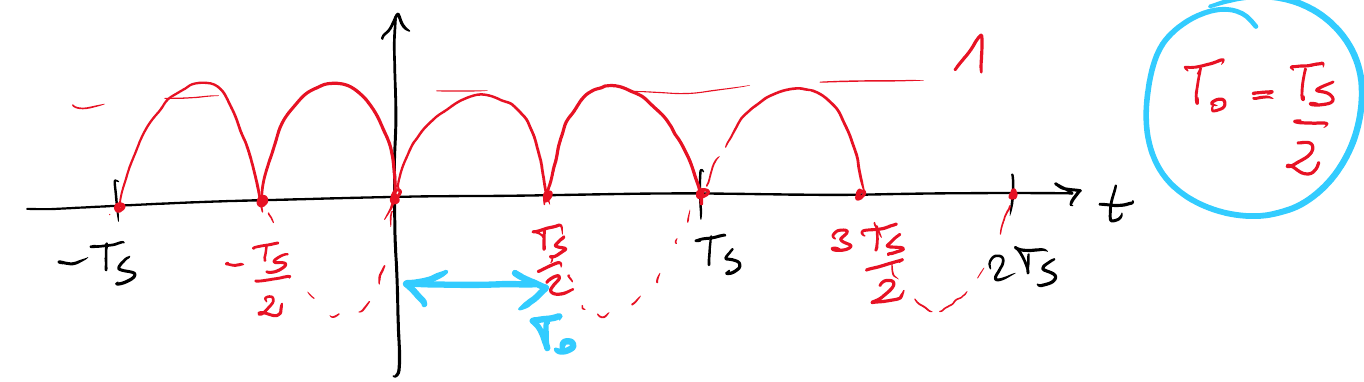
\includegraphics[scale=0.35]{immagini/lez4/grafico.jpg}
\end{figure}

Dato che e' un segnale continuo e periodico posso applicare il teorema di Fourier, ricordando prima l'unico integrale che dobbiamo ricordarci:

\begin{equation}
    \int e^{\alpha t \, dt} = \frac{1}{\alpha} e^{\alpha t}
\end{equation}

applicando il teorema di Fourier per l'analisi:

\[\begin{split}
    a_k &= \frac{1}{T_0} \int_0^{T_0} \sin{\frac{2\pi t}{T_s}} e^{-i 2\pi F_0 k t} dt \\
    &\mbox{Formula di Eulero inversa per il seno} \\
    &= \frac{1}{T_0} \int_0^{T_0} \{ \frac{e^{\frac{i 2 \pi t}{T_s}} - e^{\frac{-i 2 \pi t}{T_s}}}{2i} \} e^{-i 2\pi F_0 k t} dt \\
    &\mbox{Spezzo l'integrale} \\
    &= \frac{1}{T_0} \int_0^{T_0} \frac{e}{2i}^{\frac{i 2 \pi t}{T_s}} e^{-i 2\pi F_0 k t} dt - \frac{1}{T_0} \int_0^{T_0} \frac{e}{2i}^{\frac{-i 2 \pi t}{T_s}} e^{-i 2\pi F_0 k t} dt \\
    &\mbox{Porto fuori il denominatore, ed unisco gli esponenti con la stessa base raccogliendo la i} \\
    &= \frac{1}{2i T_0} \int_0^{T_0} e^{i (\frac{2\pi}{T_s} - 2\pi k F_0) t}dt - \frac{1}{2i T_0} \int_0^{T_0} e^{-i (\frac{2\pi}{T_s} - 2\pi k F_0) t} dt \\
    &\mbox{Applico la formula di risoluzione del logaritmo vista prima} \\
    &= \frac{1}{2i F_0} [ \frac{e^{i 2\pi (\frac{1}{T_s}- k F_0) t}}{i 2\pi (\frac{1}{T_s} - k F_0)}] - \frac{1}{2i F_0} [ \frac{e^{-i 2\pi (\frac{1}{T_s}- k F_0) t}}{-i 2\pi (\frac{1}{T_s} - k F_0)}] \\
    &\mbox{Dopo una serie di semplificazioni} \\
    &= - \frac{1}{2 \pi (1 - 2 K)} - [e^{i 2 \pi (\frac{1 - 2k}{2}) - 1}] - \frac{1}{2 \pi (1 - 2 K)} - [e^{-i 2 \pi (\frac{1 - 2k}{2}) - 1}] \\
    -1 &= e^{i \pi (1 - 2k)} \mbox{ed } e^{-i \pi (1 + 2k)} = -1 \rightarrow \forall k \in \mathbf{N} \\
    &\mbox{possiamo quindi riscrivere il segnale}\\
    a_k &= \frac{2}{2 \pi (1 - 2k)} + \frac{2}{2 \pi (1+2k)} \\
    &= \frac{2}{\pi (1 - 4 k^2)} 
\end{split}\]

Ma dato che sappiamo un segnale periodico avere infinite componenti lo scriviamo come sommatoria:

\[
    x(t) = \sum_{k = - \infty}^{+\infty} \frac{2}{\pi (1 - 4 k^2)} e^{-i 2\pi F_0 k t}
\]

\section{Condizioni sufficienti di esistenza della serie di Fourier}

Dirichlet si e' inventato delle condizioni di esistenza della serie di Fourier. Noi diremo piu' semplicemente che la serie esiste sempre, in quanto vedremo che le condizioni poste sono sufficientemente ampie, di conseguenza, dato che trattiamo segnali reali, ogni segnale che vedremo le rispettera'.

\subsection{$x(t)$ assolutamente sommabile}
Significa che e' possibile calcolare l'integrale sul periodo del segnale, il risultato dell'integrale dev'essere un numero C minore di infinito. 
E' una cosa che con i segnali reali succede sempre, non esiste un segnale che converge a piu' infinito.

\begin{equation}
    \int_0^{T_0} |x(t)| d t = C < + \infty
\end{equation}

\begin{figure}[ht!]
    \centering
    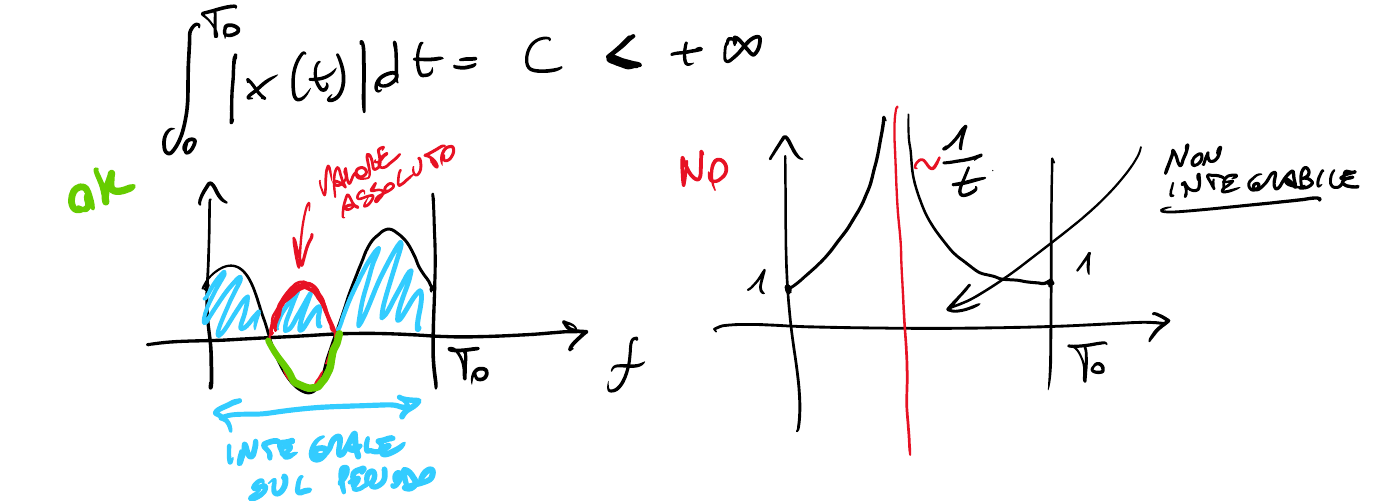
\includegraphics[scale=0.35]{immagini/lez5/assolutamenteSommabile.jpg}
\end{figure}

\subsection{$x(t)$ ha un numero finito di estremi (massimi e minimi, nel periodo)}

\begin{figure}[ht!]
    \centering
    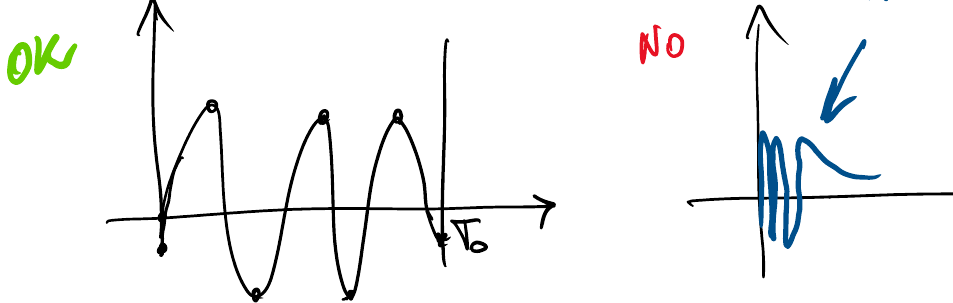
\includegraphics[scale=0.35]{immagini/lez5/finitoMassimi.jpg}
\end{figure}

I segnali che non rispettano questa proprieta' hanno un andamento del tipo $\sin{\frac{1}{x}}$ in quando oscillano infinito volte avvicinandosi ad un punto.

\subsection{$x(t)$ ha un numero di discontinuita' finite e dev'essere finito (nel periodo)}
Con discontinuita' intendiamo salti e semplicemente significa che la funzione deve avere un numero finito di salti ed ogni salto dev'essere finito.
Anche in questo caso ogni segnale reale rispetta questa proprieta'.

\begin{figure}[ht!]
    \centering
    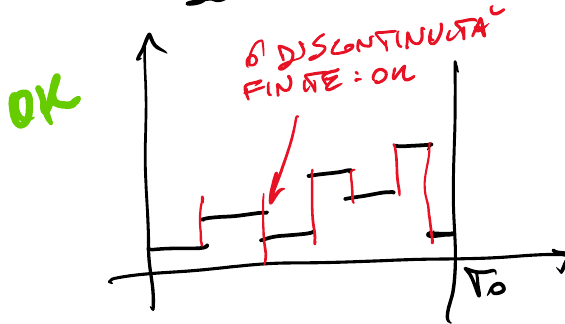
\includegraphics[scale=0.35]{immagini/lez5/discontinuitaFinite.jpg}
\end{figure}

Trovare un segnale che non rispetta questa proprieta' e' difficile, esiste pero' il segnale di cantor, che e' un segnale costruito dal seguente algoritmo:
\begin{enumerate}
    \item $T_0 = 1$ e $X_0(t) = 1$
    \item Dividi $X_i (t)$ in tre parti dove vale 1
    \item Aggiungi a quella centrale -1 per ottenere $X_i+1 (t)$
\end{enumerate}

e si ottiene questo segnale

\begin{figure}[ht!]
    \centering
    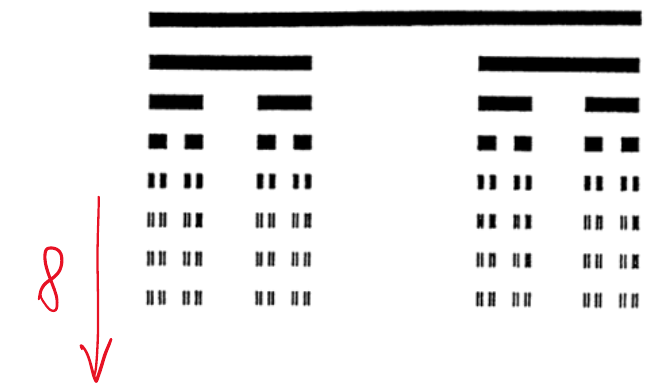
\includegraphics[scale=0.35]{immagini/lez5/cantorSet.jpg}
\end{figure}


\section{Figura di riassunto}

\begin{figure}[ht!]
    \centering
    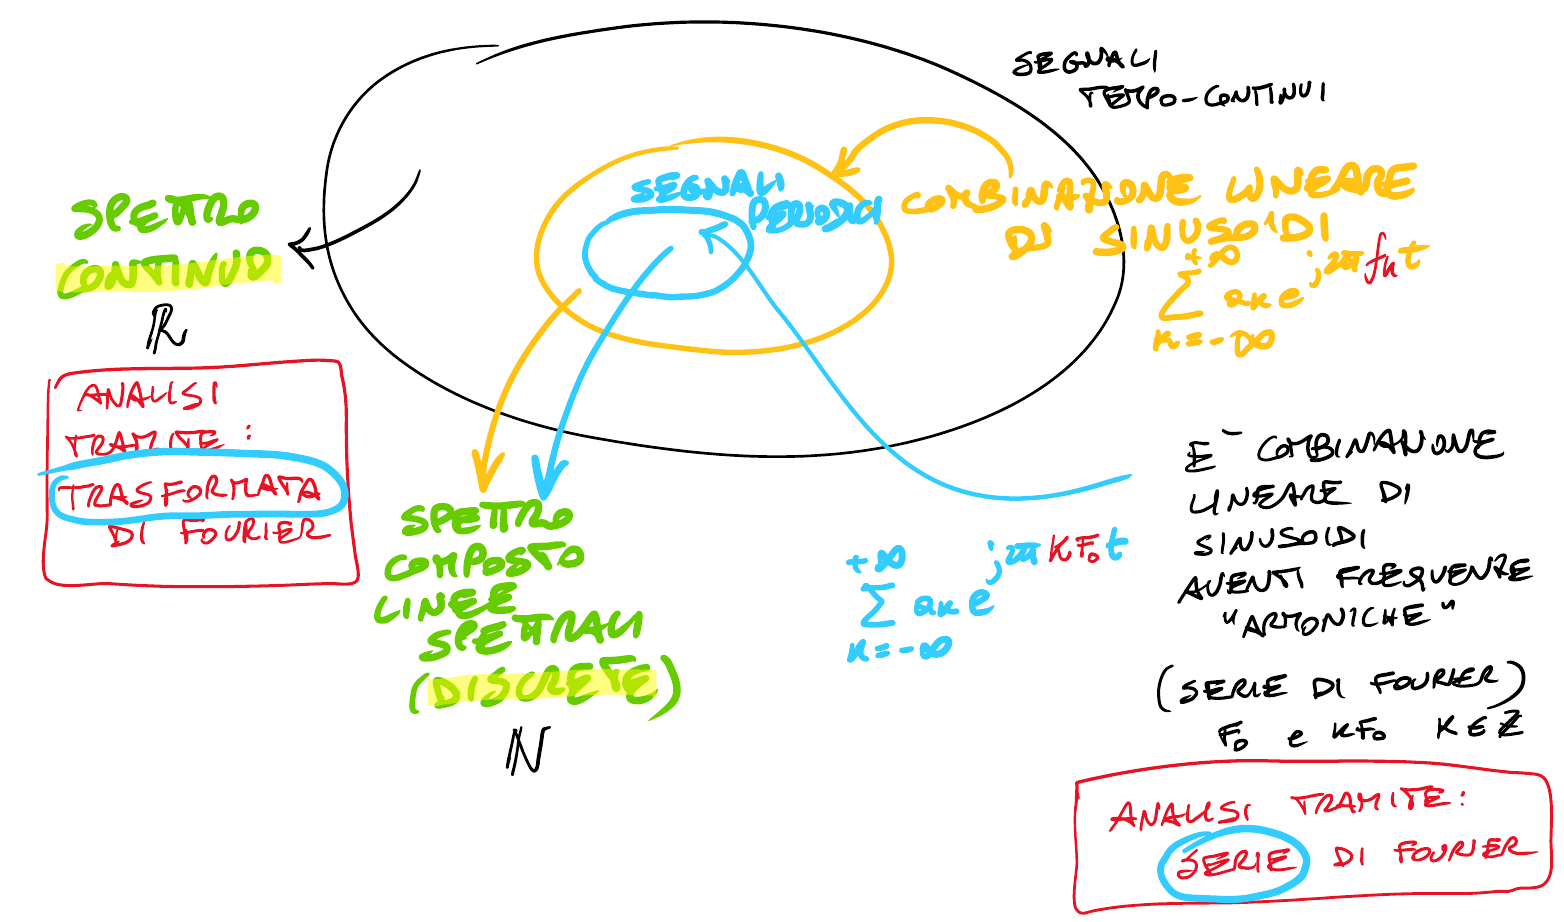
\includegraphics[scale=0.35]{immagini/lez5/schemaRiassuntivo.jpg}
\end{figure}

Si dice che i segnali appartenenti all'insieme R hanno lo spettro con la stessa potenza dei reali, allo stesso modo i segnali appartenenti all'insieme N hanno lo spettro con la stessa potenza dei numeri naturali.

\section{Trovare frequenza fondamentale date delle armoniche}
Capiamo ora quando ci viene dato un segnale composto da piu' frequenze a capire se le frequenze da cui e' composto sono armoniche.
Semplicemente date delle frequenze prendiamo il Minimo Comune Denominatore, il quale oltre a dimostrare il fatto che le frequenze sono arminche tra di loro e' anche la frequenza fondamentale $F_0$.

\subsection{Esempio 1}
Date le seguenti frequenze:
\begin{itemize}
    \item $f_1 = 16$ Hz
    \item $f_2 = 24$ Hz
    \item $f_3 = 40$ Hz
\end{itemize}

Cerchiamo di capire se sono frequenza armoniche.
Inizialmente le scomponiamo in fattori primi:
\begin{itemize}
    \item $f_1 = 2^4$
    \item $f_2 = 2^3 \cdot 3$
    \item $f_3 = 2^3 \cdot 5$
\end{itemize}

Da questa scomposizione prendiamo il MCD $2^3$ che sara' quindi la frequenza fondamente $F_0 = 2^3 \mbox{Hz}$ che ci dimostra il fatto che le frequenze sono armoniche.
Dalla frequenza fondamentale possiamo che ricavare il periodo base $T_0 = \frac{1}{8} 5$.
A questo punto possiamo esprimere le frequenze in funzione della frequenza fondamentale, dividendo la frequenza per la frequenza principale, capendo quindi di quale armonica si tratta:

\begin{itemize}
    \item $f_1 = 2 \cdot F_0 \rightarrow \, 2^a\mbox{ armonica}$
    \item $f_2 = 3 \cdot F_0 \rightarrow \, 3^a\mbox{ armonica}$
    \item $f_3 = 5 \cdot F_0 \rightarrow \, 5^a\mbox{ armonica}$
\end{itemize}

\subsection{Esempio 2}
Date le frequenze:
\begin{itemize}
    \item $f_1 = 31$ Hz
    \item $f_2 = e^1$ Hz
    \item $f_3 = \pi$ Hz
\end{itemize}

possiamo subito dire, dato che alcune frequenze sono numeri irrazionali non e' possibile che siano multipli di un numero comune, di conseguenza il segnale composto da queste frequenze non e' periodico.

\subsection{Esempio 3}
Date le frequenze:
\begin{itemize}
    \item $f_1 = \cos{(4 \pi t)}$ Hz
    \item $f_2 = \cos{(\frac{8}{5} \pi t)}$ Hz
    \item $f_3 = \cos{(\frac{16}{5} \pi t)}$ Hz
\end{itemize}

%da finire ma perche' non l'ho capito, come passa alle frazioni

\section{Esempio condizioni Fourier}

Abbiamo precedentemente trovato la serie di Fourier per il seno rettificato:

\[\begin{split}
    &x(t) = |\sin{\frac{2 \pi t}{T_s}}| \\
    &\mbox{Serie di Fourier:} \\
    &x(t) = \sum_{k = - \infty}^{+ \infty} \frac{2}{\pi (1 - 4 k^2)} e^{-j 2\pi t k \frac{2}{T_s}} \\
    &T_0 = \frac{T_s}{2}\\
    &F_0 = \frac{2}{T_s}
\end{split}\]

Tracciandone il grafico:

\begin{figure}[ht!]
    \centering
    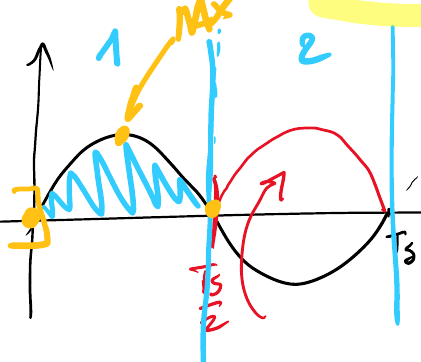
\includegraphics[scale=0.5]{immagini/lez6/sinRettificato.jpg}
\end{figure}

Ma rispetta le condizioni di esistenza?
\begin{enumerate}
    \item L'integrale nel periodo e' un numero in quanto la funzione e' finita
    \item Ho un numero finito di estremi, nel nostro caso 1 massimo ed 1 minimo
    \item Ho un numero finito di dinscontinuita', non ne ho
\end{enumerate}

Disegniamo adesso data la serie di Fouerier i grafici del segnale, del modulo e della fase.
Per farlo diamo semplicemente dei valori a k e vediamo cosa succede a $a_k$ ed a $f_k$, ricordandoci che $a_k = \frac{2}{\pi (1-4 k^2)}$ e $f_k = k F_0$.

\begin{figure}[ht!]
    \centering
    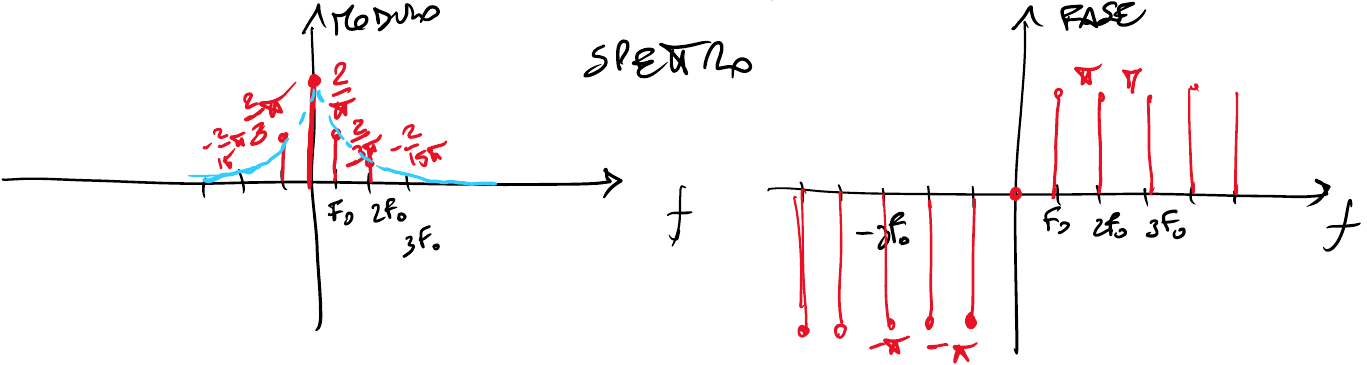
\includegraphics[scale=0.35]{immagini/lez6/moduloFaseSinRettificato.jpg}
\end{figure}

L'intuizione che abbiamo e' che dobbiamo per forza troncare la sommatoria ad un certo punto, in quanto non possiamo nella realta' continuare a sommare a $+ \infty$.

\section{Esempio Pulse Wave}

Consideriamo adesso questo segnale, chiamato Pulse Wave (o ad impulsi).
Che ha periodo $1 \rightarrow T_0$, ha la caratteristica di valere 1 per un tempo $\tau <T_0$ e 0 il resto del tempo. Inoltre un'altra caratteristica e' il duty cicle, ovvero quanto tempo e' acceso e spento (vale o 1 o 0), che e' dato da $\frac{\tau}{T_0}$.

\begin{figure}[ht!]
    \centering
    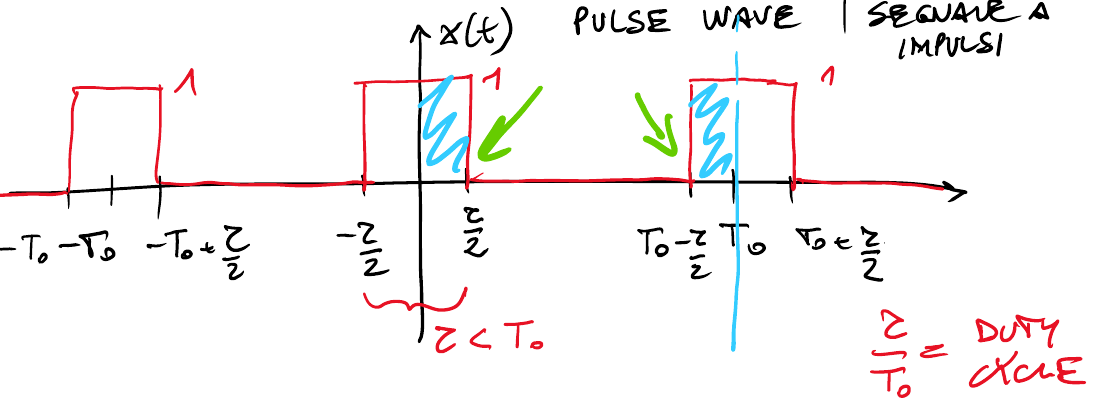
\includegraphics[scale=0.35]{immagini/lez6/pulseWave.jpg}
\end{figure}

Rispetta le condizioni di Dirichlet?
\begin{itemize}
    \item $\int_0^{T_0} |x(t)| dt = \tau < + \infty$. L'integrale nel periodo e' un numero finito
    \item Ho un numero finito di massimi e minimi, la funzione vale o 1 o 0
    \item Ho un numero finito di discontinuita', 2.
\end{itemize}

Allora se rispetta tutte le condizioni deve esistere una serie di Fourier, di cui :
\[\begin{split}
    a_k =
  \begin{cases}
    \frac{\tau}{T_0} & \text{se } k = 0 \\
    \frac{\sin{(\pi F_0 k \tau)}}{\pi k}    & \text{se } k \neq 0\\
  \end{cases}
  \, \mbox{ ed  }F_0 = \frac{1}{T_0}
\end{split}\]

Notiamo disegnando il grafico del modulo che il segnale converge a 0 piu' e' grosso il duty cicle.

\begin{figure}[ht!]
    \centering
    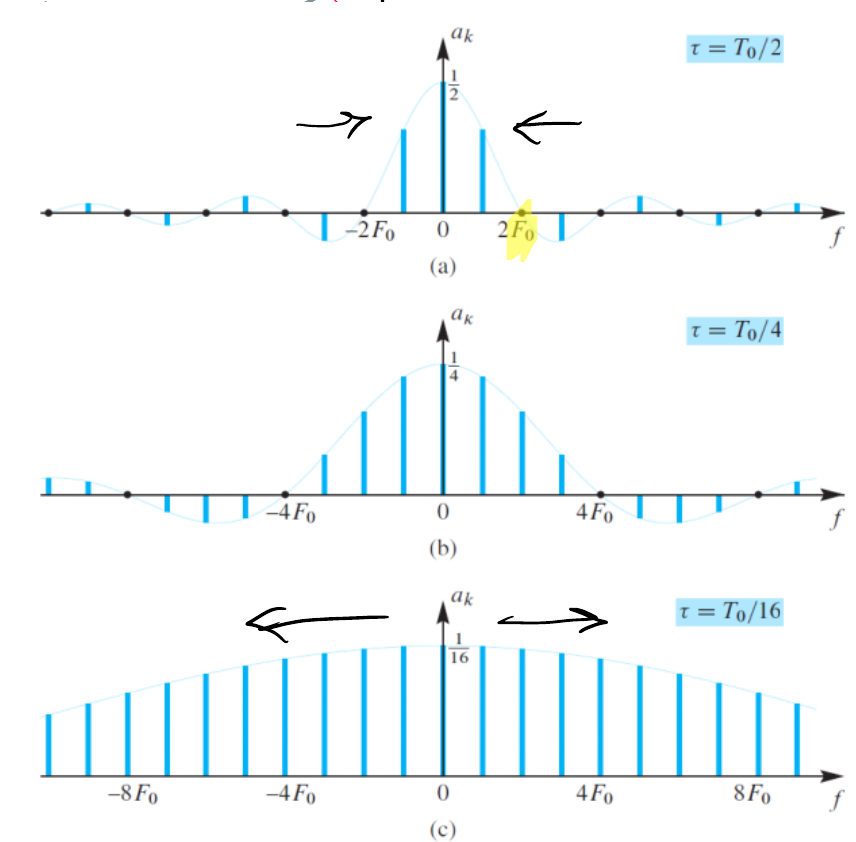
\includegraphics[scale=0.40]{immagini/lez6/manipolazionePulseWave.jpg}
\end{figure}

Introduciamo la definizione di seno cardinale (SINC) in modo da poter riscrivere la serie di Fourier in termini del seno cardinale:

\begin{equation}
    sinc(t) =
  \begin{cases}
    1 & \text{se } t = 0 \\
    \frac{\sin{(t)}}{t}   & \text{se } t \neq 0 
  \end{cases}
\end{equation}

Possiamo quindi riscrivere il segnale Pulse Wave:

\[
    x(t) = \sum_{k = - \infty}^{+ \infty} sinc(\pi F_0 k \tau) e^{-i2 \pi t k F_0}
\]

\section{Ricostruzione (sintesi o troncamento) parziale della serie di Fourier}
Sappiamo che il teorema di Fourier garantisce:
\[
    x(t) = \sum_{k = - \infty}^{+ \infty} a_k e^{-i2 \pi t k F_0}
\]

ci chiediamo ora cosa succede quando sommiamo non da meno a piu' infinito ma da $-N$ a N (non tronchiamo mai in modo asimmetrico, quindi prendiamo gli opposti).

\[
   \Tilde{x}(t) = \sum_{k = -N}^{N} a_k e^{-i2 \pi t k F_0}
\]

Come quantifichiamo un errore nel troncamento?

\subsection{Errore Massimo}
\[\begin{split}
    E_{MAX} = &MAX|x(t) - \Tilde{x}(t)| \\
    &t \in [0; T_0)
\end{split}\]

Quindi l'errore massimo e' la differenza tra il segnale originale ed il segnale ricostruito tramite la serie di Fourier con N termini.
Ovviamente l'errore variera', ma se $x(t)$ contiene una o piu' discontinuita' finite, allore l'errore massimo sara' di circa il $9\%$ dell'ampiezza della discontinuita'. Questa proprieta' si chiama fenomeno di Gibbs, ed e' presente solo se il segnale contiene una o piu' discontinuita' finite.

\subsection{Errore (quadratico) medio}

Come in statistica calcoliamo l'errore quadratico medio (varianza).

\[
    \epsilon_M^2 = \frac{1}{T_0} \int_0^{T_0} |x(t) - \Tilde{x}(t)|^2 dt
\]

Dividiamo per $T_0$ per fare la media degli errori, inoltre ricordiamo che dobbiamo fare l'integrale perche' e' il modo di sommare nei tempi continui.

L'errore medio non ci da informazioni sull'errore massimo, quindi ipoteticamente potrebbe esserci sempre un errore basso e poi in un istante un errore altissimo, il segnale medio non ci da informazioni su questa cosa.

\subsubsection{Teorema di Parseval (legge di conservazione)}
Ci serve questo teorema per poi trovare un modo per quantificare l'errore medio.
In pratica mette in relazione l'integrale del quadrato del segnale con la somma dei coeficenti della serie di Fourier, quello che facciamo e' passare dal dominio del tempo al dominio delle frequenze.

\begin{equation}
    \frac{1}{T_0} \int_0^{T_0} |x(t)|^2 dt = \sum_{k = - \infty}^{+ \infty} |a_k|^2
\end{equation}

Il primo termine e' la potenza di un segnale tempo continuo a periodico, mentre gli $a_k$ sono i coeficenti della serie di Fourier, che quindi implicitamente deve esistere.

\subsection{Errore quadratico medio con Parseval}

A questo punto posso riscrivere l'errore quadratico medio, che ricordiamo essere:

\[
    \epsilon_M^2 = \frac{1}{T_0} \int_0^{T_0} |x(t) - \Tilde{x}(t)|^2 dt
\]

utilizzando il teorema di Parseval, trasformando quindi l'integrale in sommatoria dei coeficienti, posso riscrivere il segnale:

\[\begin{split}
    x(t) &= \sum_{k = - \infty}^{+ \infty} a_k e^{-j2 \pi t F_0 k} \\
    \Tilde{x}(t) &= \sum_{k = -N}^{+ N} a_k e^{-j2 \pi t F_0 k} \\
    e(t) &= \sum_{k = - \infty}^{+ \infty} a_k e^{-j2 \pi t F_0 k} - \sum_{k = -N}^{+ N} a_k e^{-j2 \pi t F_0 k}
\end{split}\]

Facendo la differenza tra le due sommatorie, dato che i coeficienti con N saranno uguali in tutte e due le sommatorie, facendone la differenza e' come se tenessimo tutti i termini da $-\infty \rightarrow N$ e da $N \rightarrow +\infty$:

\[
    \sum_{k = - \infty}^{-N -1} a_k e^{-j2 \pi t F_0 k} - \sum_{k = N+1}^{+ \infty} a_k e^{-j2 \pi t F_0 k}
\]

Lo spettro del segnale sara':

\[
    e(t) =
  \begin{cases}
    0 & \text{se } -N \le K < N \\
    a_k   & \text{Altrimenti } 
  \end{cases}
\]

Concludendo l'errore quadratico medio nella sintesi parziale e' pari alla somma del modulo quadro dei coeficienti $a_k$ (della serie di Fourier) scartati.

Anche nel fuzzy wave i coeficenti tendono a 0, quindi l'errore medio diminiusce man mano che i coeficienti aumentano (sommo piu' segnali).

Nel segnale del seno rettificato l'errore medio e':

\[
    |\sin{(\frac{2\pi t}{T_s})}| \rightarrow \lim_{x\to\infty} |a_k| \approx \frac{1}{k^2}
\]

mentre nel segnale fuzzy wave:

\[
    a_k \approx \frac{1}{k}
\]

\section{Collocamento}
Parliamo di collocamento temporale nel senso in cui un segnale si dice ben collocato nel tempo se succede in un tempo molto piccolo, ad esempio un esplosione. Mentre un evento (segnale) si dice non collocato nel tempo se succede per la maggior parte del tempo, ad esempio la luce durante la giornata.

Quello che ci interessa e' che se il segnale ha un collocamento stretto (e' un evento in un tempo piccolo) allora serviranno tante frequenze per descriverlo, viceversa se largo.
Questa cosa l'abbiamo notata cambiano di duty cicle del segnale fuzzy wave, notando che piu' era alta piu' l'ampiezza del segnale diminuiva, e viceversa.

\section{Dualita' tempo-frequenza}
Partiamo parlando di come nei secoli l'uomo ha voluto scrivere la musica per poterla trasportare, lo facciamo rappresentando le note (che sono un suono), indicandone graficamente la frequenza e la durata:

\begin{figure}[ht!]
    \centering
    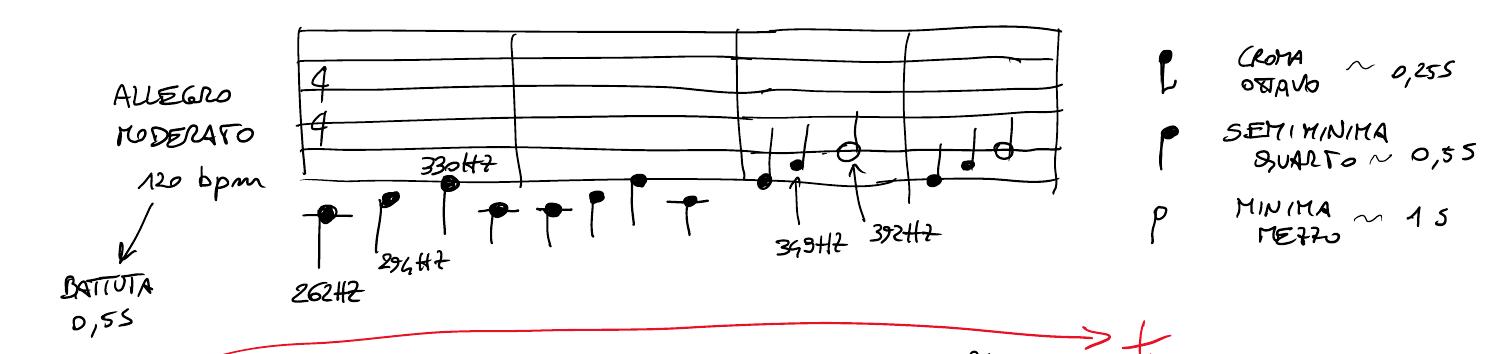
\includegraphics[scale=0.35]{immagini/lez7/campanaro.jpg}
\end{figure}

Dello spartito possiamo rappresentare il grafico del modulo (dello spettro dei segnali), e vedere come cambiano i moduli nel tempo:

\begin{figure}[ht!]
    \centering
    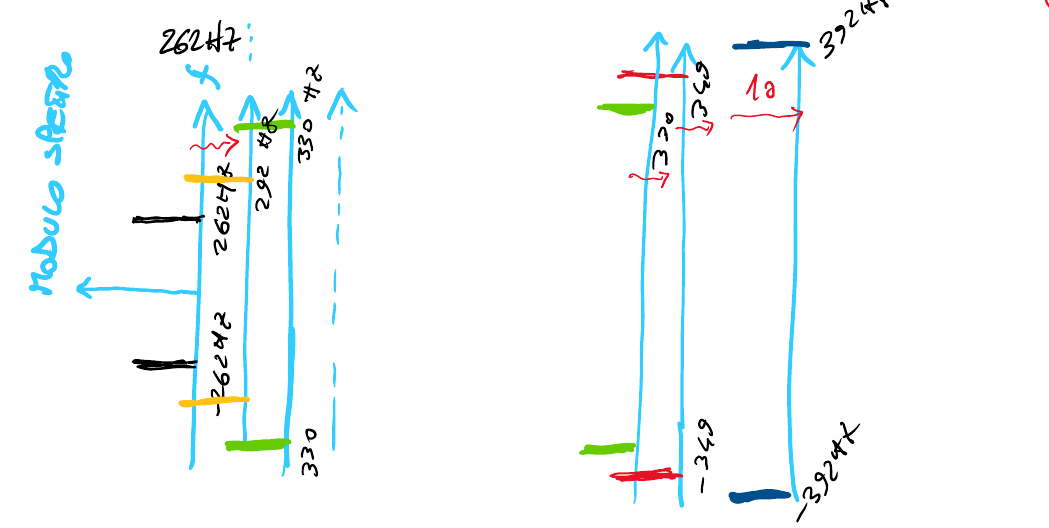
\includegraphics[scale=0.35]{immagini/lez7/graficoModuloTempo.jpg}
\end{figure}

Da quello che abbiamo visto fino ad ora possiamo rappresentare in forma trigonometrica qualisasi nota, ad esempio il DO:

\[
    A \cos{(2\pi 262 \cdot t)}
\]

Dove A e' l'ampiezza del segnale, in quando potremmo suonare un DO piu' o meno forte, mentre l'argomento del coseno e' il segnale emesso da uno strumento musicale. Pero' rappresentato in questo modo durerebbe all'infinito, cosa che intuitivamente sappiamo non essere possibile in realta', quindi prima o poi deve fermarsi.
Cio'nonostante noi possiamo considerare il segnale emesso in un preciso istante e considerarlo come se fosse infinito.

Quello che dobbiamo fare per rappresentare il segnale e' aggiungere una dimensione, il tempo e per farlo dobbiamo ricondurre il segnale al suo spettro, perche' sappiamo essere il tempo e lo spettro duali ma in due dimensioni diverse.

La rappresentazione di come evolve lo spettro di un segnale nel tempo e' detta \textbf{spettrogramma}.
Ogni trattino e' quanto dura il segnale nel tempo.

\begin{figure}[ht!]
    \centering
    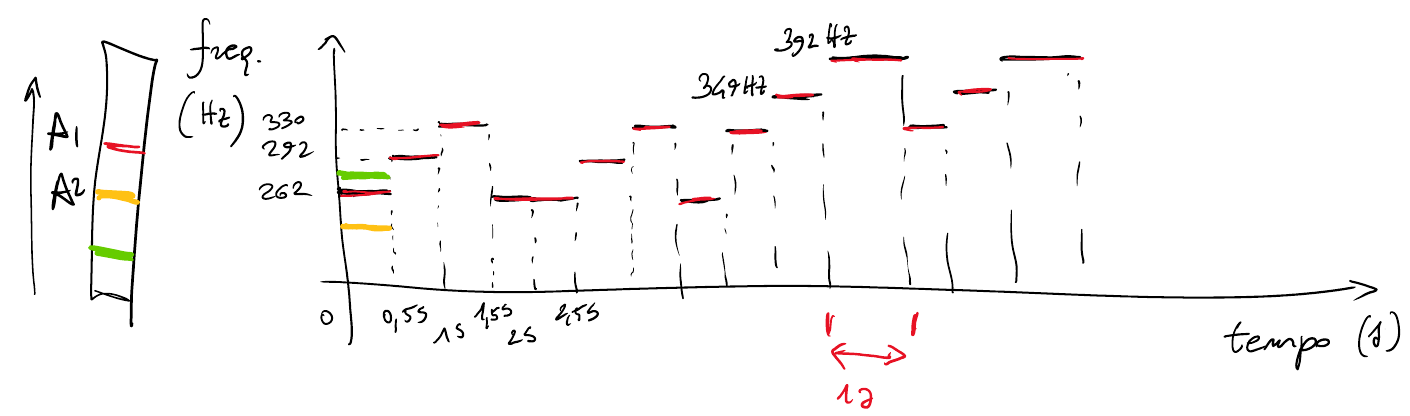
\includegraphics[scale=0.35]{immagini/lez7/spettrogramma.jpg}
\end{figure}

\section{Frequenza Istantanea}

Fino ad ora sapevamo che un segnale $\cos{2\pi f t}$ ha frequenza $f$ (ovvero le ripetizioni nel tempo). Vediamo ora dopo aver capito che dobbiamo considerare un segnale in un istante la definizione di frequenza istantanea:

\begin{equation}\begin{split}
    f_{ISTANTANEA} &= \frac{d \Theta(t)}{dt} \cdot \frac{1}{2\pi} \mbox{[Hz]} \\
    \mbox{Segnale} &= \cos{[\Theta(t)]}
\end{split}\end{equation}

Quello che dobbiamo fare in pratica e' la derivata della fase del segnale e dividerla per $2\pi$. La fase e' l'argomento nel tempo del coseno (tutto quello tra parentesi del coseno).

Dimostriamo che la definizione di frequenza istantanea coincide con quello che abbiamo fatto fino ad adesso, calcoliamo quindi la frequenza istantanea di un segnale fisso nel tempo (notiamo che $\phi = 0$ perche' il segnale non varia):

\[\begin{split}
    x(t) &= \cos{(2\pi f_0 f+ \phi)} \\
    f_{ISTANTANEA} &= \frac{d(2\pi f_0 t + \phi)}{dt} \cdot \frac{1}{2\pi} = 2\pi f_o - \frac{1}{2\pi} = f_0 
\end{split}\]

Facciamo variare adesso la frequenza istantanea nel tempo, e cerchiamo di costruire un segnale a partire dalla frequenza.

\begin{figure}[ht!]
    \centering
    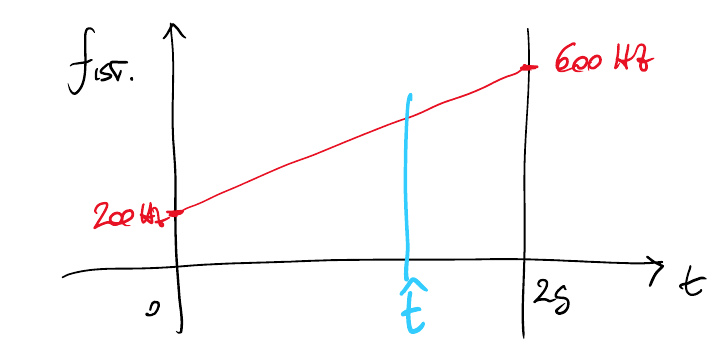
\includegraphics[scale=0.35]{immagini/lez7/fIstantaneaTempo.jpg}
\end{figure}

Dobbiamo partire dalla frequenza istantanea e costruire la fase del segnale che modula la frequenza nel tempo.
La frequenza istantanea e' l'equazione della retta (dove t e' la variabile):

\[
    f_{ISTANTANEA} = 200 + t \frac{600 - 200}{2}
\]

Ora per calcolare la fase moltiplico l'integrale tra 0 e t della frequenza istantanea per $2\pi$.

Dalla definizione precedente:

\[\begin{split}
    \Theta(t) &= \int_0^t 2\pi f_{IST} (\tau) d\tau \\
    \Theta(t) &= 2\pi \int_0^t [200 + 200 \tau] d\tau \\
    \Theta(t) &= 2\pi [200\tau + 200 \frac{\tau^2}{2}]_0^t = 200\pi [2t+t] \\
    \Tilde{x}(t) &= A \cos{[200 \pi (2t + t^2)]}
\end{split}\]

Ricordiamoci sempre che la fase non si fa mettendo direttamente la frequenza istantanea nel coseno, ma va prima integrata!

\section{Modulazione di frequenza}
Avevamo gia' visto la modulazione di ampiezza (AM), in cui il segnale trasmesso e' uguale al segnale da trasmettere moltiplicato per una portante:

\[
    x(t) = s(t) \cos{(2\pi f_0 t)}
\]

Nel caso della modulazione di frequenza (FM), ci aspettiamo che il segnale abbia un'ampiezza costante, e modulando la fase si trasmette il segnale:

\[\begin{split}
    x(t) &= a \cos{()\Theta(t)} \\
    f_{IST} &= s(t) D + F_c \\
    \Theta(t) &= 2\pi \int_0^t (s(\tau) D + F_c) \tau \rightarrow F_c >> s(t)
\end{split}\]

$F_c$ e' chiamata frequenza carrier (portante), serve per aumentare la frequenza del segnale in modo da limitare le interferenze ed e' la frequenza a cui ci sintonizziamo per ascoltare la radio. Inoltre moltiplichiamo per un'altra costante D nel caso in cui il segnale sia troppo piccolo per aumentarne l'ampiezza.


\section{Prodotto scalare di due funzioni periodiche}
Il prodotto scalare di due funzione periodiche, di periodo $T_0$:

\[
    <f(t), g(t)> \frac{1}{T_0} \int_0^{T_0} f(t) g^*(t) dt
\]

Quindi potro' dire che due funzioni sono ortogonali quando il loro prodotto scalare e' zero.

\subsection{Esempio}
Vediamo ora un esempio, calcolare il prodotto scalare tra:
\[
    <e^{i2\pi t F_o k_1}, e^{i2\pi t F_o k_2}> \rightarrow T_0 = \frac{1}{F_0}
\]

Possiamo dividere il problema in due casi, quando $k_1 = k_2$:

\[\begin{split}
    \frac{1}{T_0} &\int_0^{T_0} e^{i2\pi t F_o k} \cdot e^{-i2\pi t F_o k} dt \rightarrow = e^0 = 1 \\
    \frac{1}{T_0} &[t]_0^{T_0} = \frac{T_0}{F_0} = 1
\end{split}\]

invece quando $k_1 \neq k_2$:
\[\begin{split}
    \frac{1}{T_0} &\int_0^{T_0} e^{i2\pi t F_o k_1} \cdot e^{-i2\pi t F_o k_2} dt \\
    &\mbox{riscrivendo l'argomento dell'integrale:} \\
    &e^{i2\pi t F_0(k_1 - k_2)}\\
    &\mbox{applichiamo la formula di risoluzione dell'integrale:}\\
    \frac{1}{T_0} &[\frac{e^{i2\pi t F_0(k_1 - k_2)}}{i2\pi F_0(k_1 - k_2)}]_0^{T_0} \\
    &\mbox{risolvendo ora tra gli estremi e semplificando otteniamo:}\\
    1 &[\frac{e^{i2\pi t F_0(k_1 - k_2)}-1}{i2\pi (k_1 - k_2}] \\
\end{split}\]

Notiamo pero' che $k_1 - k_2$ sara' sempre un numero intero $\neq 0$. Quindi l'esponenziale $e^{i2\pi h} = 1$, che sottraendo con l'uno al numeratore dara' sempre 0, qualsiasi siano i valori di $k_1, k_2$.

Capito che :
\[\begin{split}
    <e^{i2\pi t F_o k_1}, e^{i2\pi t F_o k_2}> = 
    \begin{cases}
    1 & \text{se } k_1 = k_2 \\
    0   & \text{se } k_1 \neq k_2 
  \end{cases}
\end{split}\]

ci rendiamo conto che queste funzioni si comportano come somma delle basi di uno spazio vettoriale.
In uno spazio vettoriale 3D la base ortogonale standard e' composta da 3 vettori:$\Vec{i} = [100]$, $\Vec{j} = [010]$, $\Vec{k} = [001]$. Il prodotto scalare di un vettore della base con un'altro della stessa base da sempre 0, ed il prodotto scalare di un vettore della base con se stesso da sempre 1. Esattamente come succedeva per le funzioni in esempio.

Nello spazio di Fourier (le frequenze) di un segnale periodico a tempo continuo abbiamo imparato che hanno le stesse proprieta' di una base ortogonale, la differenza e' che le funzioni nello spazio di Fourier sono infinite. Come facevamo per i vettori possiamo quindi proiettare (proiezione ortogonale) ciascuna funzione sulla base e poi ricostruirla.

\chapter{Segnali a tempo discreto}
\section{Dal tempo continuo al tempo discreto}
Per arrivare a parlare dei segnali a tempo discreto cominciamo a capire come si passa da un segnale a tempo continuo ad uno a tempo discreto.

\begin{figure}[ht!]
    \centering
    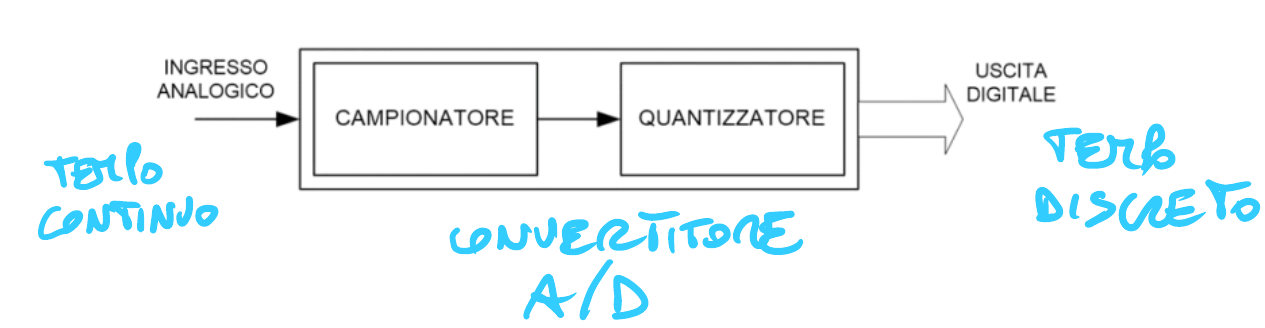
\includegraphics[scale=0.35]{immagini/lez9/convertitoreAD.jpg}
\end{figure}

Per fare questo passaggio si usa un convertitore A/D (analogico digitale) che prende in input un segnale a tempo continuo e ci fornisce in output un segnale a tempo discreto.

\subsection{Campionatore}
E' il componente del convertitore che fa il campionamento. Ho un segnale a tempo continuo e ne considero solo alcuni campioni, ad esempio se il nostro segnale e': $x(t) = A \cos{(2\pi f_0 t + \varphi_0)}$, si decide un intervallo di campionamento $T_c$ che e' in pratica la distanza tra due campioni. Di conseguenza sostituendo a t $n T_c$ si ottiene il segnale a tempo discreto:
\[
    x(\textcolor{red}{nTc}) = A \cos(2\pi f_0 \textcolor{red}{nTc} + \varphi_0)
\]

Il nostro obbiettivo sara' capire come campionare bene. Nella maggior parte dei casi campioneremo in modo uniforme, ovvero c'e' una distanza uguale tra un campione e l'altro, ma si puo' anche campionare in modo non uniforme.

\begin{figure}[ht!]
    \centering
    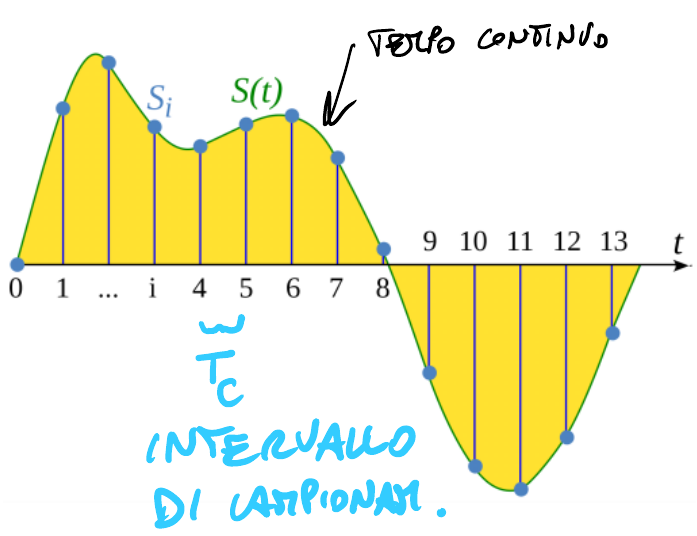
\includegraphics[scale=0.35]{immagini/lez9/campionatore.jpg}
\end{figure}

\subsection{Quantizzatore (quantizzazione)}
Possiamo considerarlo come una funzione matematica tale per cui in ingresso c'e' un segnale reale ed in uscita' c'e' un segnale che appartiene ad un sottoinsieme di numeri interi.

In pratica e' come se facessimo un arrotondamento di un decimale ad una certa posizione, facciamo un approssimazione del segnale scegliendo quanti campioni prendere.
Il least siginificant bit e' dato da : $\frac{\mbox{RANGE}}{2^{n_q}}$, dove il denominatore e' il numero di bit di quantizzazione.

\section{Osservazioni su segnali discreti}
Per fare un passo avanti per capire come campionare, analizziamo alcune caratteristiche di un segnale campionato, ovvero discreto.

Cominciamo dando della terminologia, diremo \underline{intervallo di campionamento} (espresso in secondi e costante) $T_s$ mentre diremo \underline{frequenza di campionamento} o sampling frequency $f_c = \frac{1}{T_c}$, espressa in Hz.

\subsection{La frequenza discreta e' adimensionale}
Se abbiamo un segnale tempo continuo e lo campioniamo, ricordando che $T_c = \frac{1}{f_c}$ otteniamo:
\[
    x[n] = x(n T_c) = A \cos{(2\pi f_0 \frac{n}{f_c} + \varphi_0)}
\]

Se consideriamo l'argomento del coseno in cui compare la frequenza:
\[
    \Tilde{\omega} = 2\pi \frac{f_0}{f_c}
\]

Lo chiameremo \textbf{velocita' angolare o pulsazione discreta} ed e' misurata in radianti (RAD).
Mentre se prendiamo la \textbf{frequenza discreta}:

\[
    \frac{f_0}{f_c} = \Tilde{f}
\]

e ne facciamo l'analisi dimensionale vediamo che sono Hz fratto Hz, quindi e' una grandezza adimensionale che \textbf{NON} ha niente a che vedere con il tempo.

\subsubsection{Corollario}
Un coseno tempo continuo e' sempre periodico, pero'un coseno tempo discreto non e' necessariamente periodico, perche', dato il coseno discreto definito $x[n] = \cos(2\pi \Tilde{f} n)$, se dovessimo trovare il periodo nel tempo continuo faremmo $T = \frac{1}{f}$, ma se ad esempio la frequenza discreta fosse $\frac{4}{5}$, il periodo verrebbe $\Tilde{T} = \frac{5}{4}$ che non essendo un numero interno non puo' essere un periodo.
Di conseguenza il vero periodo di una funzione a tempo discreto e' un multiplo intero del periodo ottenuto come se fossimo nel tempo continuo, moltiplicato in modo che sia un intero, nel nostro caso $\Tilde{T} = \frac{5}{4} \cdot 4 = 5$.

Se pero' $\Tilde{f}$ e' un numero irrazionale non possiamo renderlo un intero, di conseguenza esistono infinite cosinusoidi non periodiche nel tempo discreto (e se consideriamo le dimensione degli insiemi sono di piu' quelle non periodiche).

Quindi sintetizzando solo le cosinusoidi discrete che hanno $\Tilde{f}$ (frequenza) che e' un numero razionale sono periodiche.

\subsection{Segnali diversi campionati a frequenze diverse possono dare lo stesso segnale}
Consideriamo tre segnali a tempo continuo diversi, campioniamoli con una frequenza di campionamento ($f_s$) diversa e vediamo che segnale a tempo discreto otteniamo:

\[\begin{split}
    x_1(t) &= \cos(2\pi 200t) \rightarrow f_s = 1000\mbox{Hz} \rightarrow x[n] = \cos(s\pi 200 \frac{n}{1000}) = \cos(2\pi \frac{n}{5}) \\
    x_2(t) &= \cos(2\pi 100t) \rightarrow f_s = 500\mbox{Hz} \rightarrow x[n] = \cos(s\pi 100 \frac{n}{500}) = \cos(2\pi \frac{n}{5}) \\
    x_3(t) &= \cos(2\pi 1000t) \rightarrow f_s = 5000\mbox{Hz} \rightarrow x[n] = \cos(s\pi 1000 \frac{n}{5000}) = \cos(2\pi \frac{n}{5}) \\
\end{split}\]

Da questo notiamo che abbiamo ottenuto sempre lo stesso segnale, dato che la frequenza di campionamento e' adimensionale puo' capitare, come in questo caso, che campionando segnali diversi con frequenze diverse il risultato sia lo stesso segnale.

Questo ci fa intuire che se vogliamo tornare indietro dobbiamo sapere le diverse frequenze di campionamento, altrimenti sarebbe impossibile distinguere a quale segnala appartiene il segnale campionato.

\begin{figure}[ht!]
    \centering
    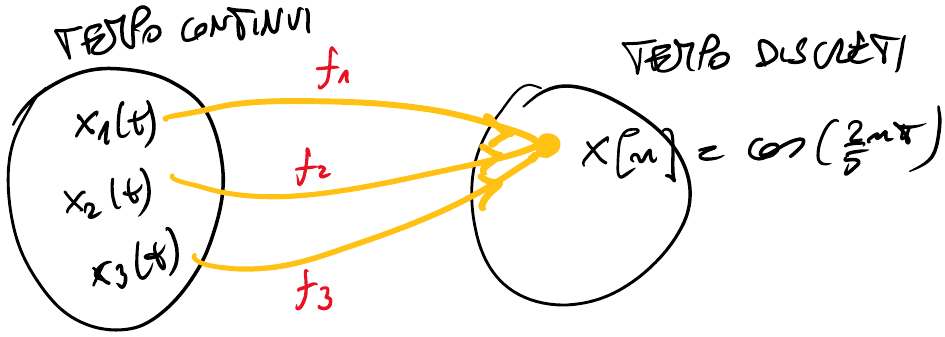
\includegraphics[scale=0.35]{immagini/lez9/stessoSegnale.jpg}
\end{figure}

\subsection{Ogni coseno discreto ha infiniti ALIAS SECONDARI, ma uno PRINCIPALE nell'intervallo}

Dato un segnale a tempo discreto, che chiamiamo ALIAS PRINCIPALE, posso costruire un altro segnale discreto identico ma con i termini diversi, che chiamiamo ALIAS SECONDARIO:

\[\begin{split}
    x_1[n] &= \cos(\frac{2}{5} \pi) = \cos(0,4 \pi n) \\
    x_2[n] &= \cos(0,4 \pi n + 2\pi n) = \cos(2,4 \pi n) =  \cos(0,4 \pi n) \\
    x_3[n] &= \cos(0,4 \pi n - 2\pi n) = \cos(-1,6 \pi n) =  \cos(1,6 \pi n) \\
\end{split}\]

Quindi ogni coseno discreto ha infiniti alias secondari, ma uno principale nell'intervallo $(-\pi]$, cioe' sappiamo quindi che la velocita' angolare $\Tilde{\omega}$ deve appartenere a questo intervallo. Espresso in termini di frequenza, sappiamo che la frequenza discreta $\Tilde{f} \in [-\frac{1}{2}, \frac{1}{2})$.

Nel mondo reale la frequenza puo' crescere all'infinito, mentre nel discreto non puo' mai superare $0,5$ altrimenti si ottiene un alias secondario del segnale originale.

\begin{table}[ht!]
    \centering
    \begin{tabular}{c|c|c|c|c}
         & $\cos(0,4 \pi n)$ & $\cos(2,4 \pi n)$ & $\cos(-0,4 \pi n)$ & $\cos(1,6 \pi n)$ \\
         \hline
        n=1 & 0,3090 & 0,3090 & 0,3090 & 0,3090 \\
        n=2 & -0,8090 & -0,8090 & -0,8090 & -0,8090 \\
        n=3 & -0,8090 & -0,8090 & -0,8090 & -0,8090 \\
        n=4 & 0,3090 & 0,3090 & 0,3090 & 0,3090 \\
        n=5 & 1,0000 & 1,0000 & 1,0000 & 1,0000 \\
    \end{tabular}
\end{table}

\subsubsection{Folded Alias}
Se trovo un'alias secondario che ha un segno negativo, posso spostare quel meno alla fase, ottenendo cosi' un Folded Alias, ovvero un alias con la fase cambiata di segno.

\[
    \cos(0,4 \pi n + \varphi) = \cos(\textcolor{red}{-}  1,6 \pi n + \varphi) = \cos(1,6 \pi n \textcolor{red}{-} \varphi)
\]

E se tolgo quel meno dalla fase trasformandolo in un complesso ottengo:
\[
    \cos(0,4 \pi n + \varphi + 2\pi h n) \rightarrow h \in \mathbf{Z}
\]

\section{Spettro}
Vediamo ora come ottenere lo spettro di un segnale tempo discreto.
Lo facciamo decomponendo il coseno con la formula di Eulero inversa:

\[
    x_1[n] = \cos(2\pi \Tilde{f} n + \varphi) = \frac{1}{2} e^{i \varphi} \cdot e^{i 2\pi \Tilde{f} n} + e^{-i \varphi} \cdot e^{-i 2\pi \Tilde{f} n}
\]

Il grafico del modulo dello spettro e':

\begin{figure}[ht!]
    \centering
    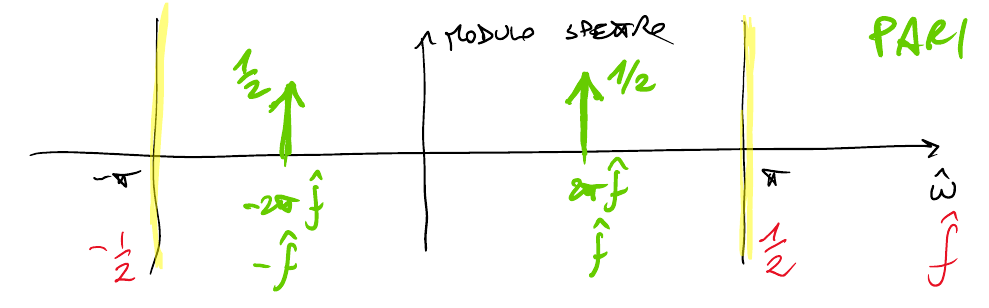
\includegraphics[scale=0.35]{immagini/lez10/spettroDiscreto.jpg}
\end{figure}

Ricordiamo che per essere formali, quando passiamo nel discreto disegno delle frecce e non solo barre, sia nel grafico del modulo che della fase.

Consideriamo ora un'altro segnale, che sappiamo essere un alias di quello precedente:

\[
    x_2[n] = \cos(2\pi \Tilde{f} n + \varphi + 2\pi n) = \frac{1}{2}e^{i \varphi} \cdot e^{i(2\pi \Tilde{f} + 2\pi)n} + \frac{1}{2}e^{-i \varphi} \cdot e^{-i(2\pi \Tilde{f} + 2\pi)n}
\]


Notiamo che nonostante i segnali siano degli alias hanno dei grafici diversi, questo perche' lo spettro di un segnale tempo discreto e' periodico, quindi contiene "righe" periodiche ($T = 2\pi$), che sono tutti gli spettri degli alias.

Questo ci fa intuire che l'unico segnale che posso ricostruire dato lo spettro e' l'alias principale (esempio frazioni).

\subsection{Esempio}
Abbiamo un segnale tempo continuo da campionare, provo varie frequenze di campionamento per vedere quale posso usare per ricostruire il segnale.

\[
    x(t) = \cos(2\pi \cdot 100t + \frac{\pi}{3})
\]

La prima frequenza di campionamento e' $f_s = 500$Hz:

\[
    x[n] = 2\cos(2\pi 100 \frac{n}{500} + \frac{\pi}{3}) = 2\cos(\frac{2\pi}{5} n + \frac{\pi}{3})
\]

Ora ricavo lo spettro:

\[
    x[n] = 1e^{i \frac{\pi}{3}} e^{i \frac{2}{5}\pi n} + 1e^{-i \frac{\pi}{3}} e^{-i \frac{2}{5}\pi n}
\]

Il grafico del modulo:

\begin{figure}[ht!]
    \centering
    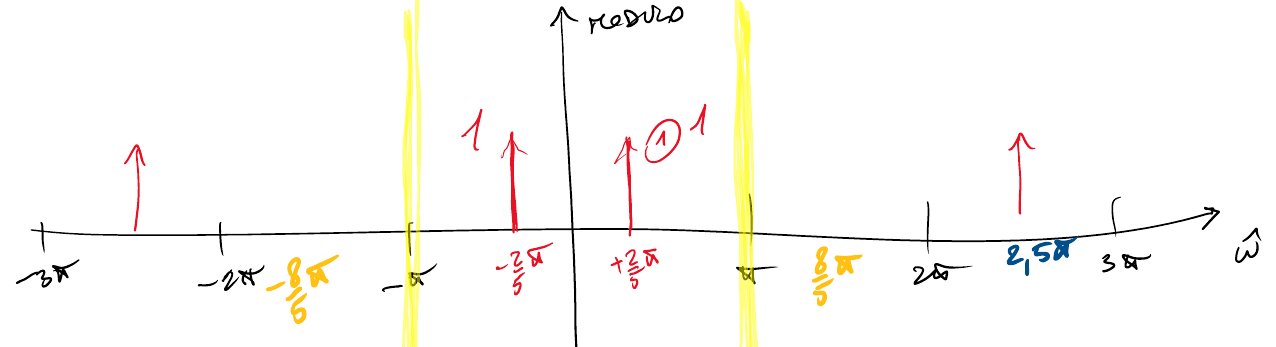
\includegraphics[scale=0.35]{immagini/lez10/moduloEsempio.jpg}
\end{figure}

Dal grafico noto che e' ottenuto l'alias principale, in quanto il modulo sta tra $-\pi, \pi$.
Quindi ricordando che $t = n \cdot T_c = \frac{n}{T_c}$ e che $n = t \cdot T_c$ posso ricostruire l'alias principale: 

\[
    x[t \cdot f_c] = 2\cos(\frac{2\pi}{5} \cdot t 500 + \frac{\pi}{3})
\]

Usiamo ora come frequenza di campionamento $f_s = 125$Hz:
\[
    x[n] = 2\cos(2\pi 100 \frac{n}{125}) = 2\cos(\frac{2\pi}{5} 4 n)
\]

tracciando il grafico:

\begin{figure}[ht!]
    \centering
    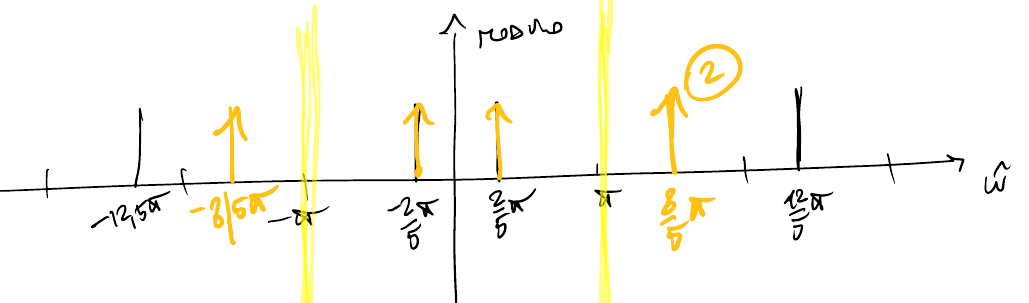
\includegraphics[scale=0.35]{immagini/lez10/moduloEsempio2.jpg}
\end{figure}
Noto che abbiamo ottenuto un'alias secondario, calcolo quindi quello principale:

\[
    x[n] = \cos(\frac{8}{5}\pi n + \frac{\pi}{3}) = \cos(\frac{8}{5} \pi n + \frac{\pi}{3} - 2\pi n) = \cos(-\frac{2}{5}\pi n + \frac{\pi}{3}) = \cos(\frac{2}{5} \pi n + \frac{\pi}{3})
\]

Posso quindi ricostruire solo l'alias principale (sostituendo ad n $t \cdot f_s$:

\[
    x[t \cdot f_s] = \cos(\frac{2}{5} \pi t 125 + \frac{\pi}{3})
\]

Usiamo ora come frequenza di campionamento $f_s = 100$Hz:

\[
    x[n] = 2\cos(2\pi 100 \frac{n}{100} + \frac{\pi}{3}) = 2\cos(2 \pi  n + \frac{\pi}{3})
\]

tracciando il grafico:

\begin{figure}[ht!]
    \centering
    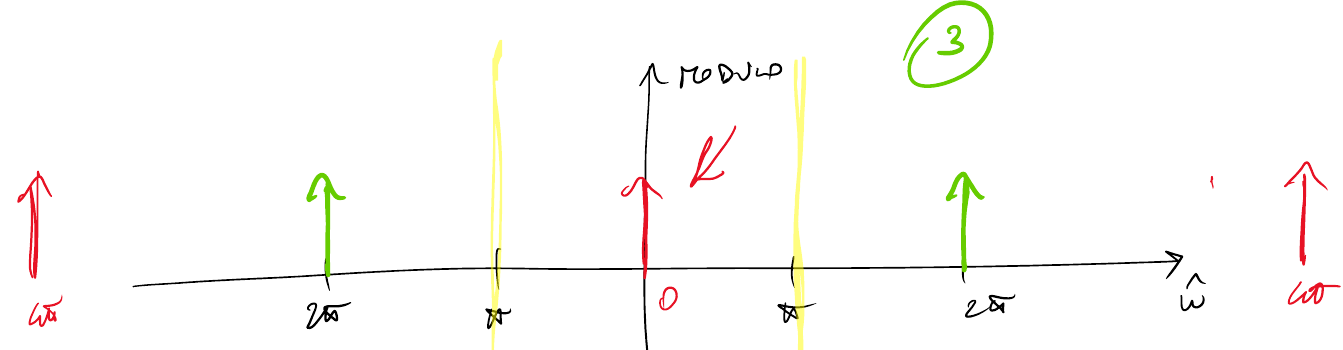
\includegraphics[scale=0.35]{immagini/lez10/moduloEsempio3.jpg}
\end{figure}
Noto che abbiamo ottenuto un'alias secondario, calcolo quindi quello principale:

\[
    x[n] = 2\cos(2\pi n + \frac{\pi}{3}) = 2\cos(\frac{\pi}{3}) \rightarrow x(t) = 2\cos(\frac{\pi}{3})
\]

Come ultimo esempio usiamo la frequenza di campionamento $f_s = 80$ Hz, da cui, come fatto fino ad ora, otteniamo il segnale campionato:

\[
    x[n] = 2\cos(2\pi 100 \frac{n}{80} + \frac{\pi}{3}) = 2\cos(2\pi \frac{5n}{4} + \frac{pi}{3})
\]

Tracciandone il grafico del modulo:

\begin{figure}[ht!]
    \centering
    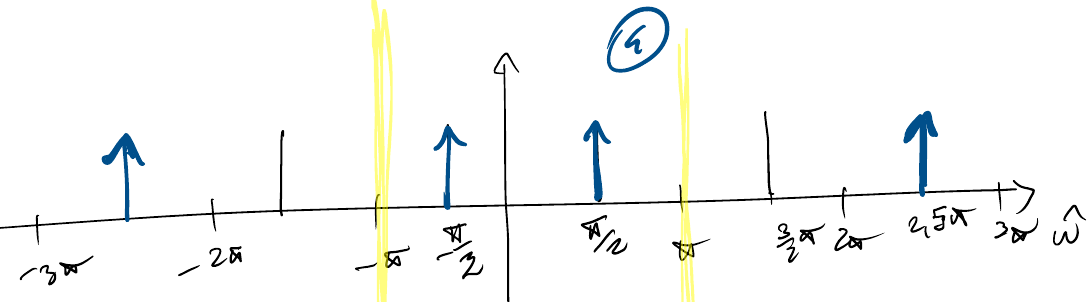
\includegraphics[scale=0.35]{immagini/lez10/moduloEsempio4.jpg}
\end{figure}

Notiamo ancora una volta che abbiamo ottenuto un alias secondario, quindi otteniamo quello principale e poi ricostruiamo il segnale:

\[
    x[n] = 2\cos(\frac{5}{2}\pi n + \frac{\pi}{3}) = 2\cos(\frac{\pi}{2} n + \frac{\pi}{3}) \rightarrow x(t) = 2\cos(\frac{\pi}{2} 80 t + \frac{\pi}{3}) = 2\cos(2\pi 20 t + \frac{\pi}{3})
\]

Le cose che dobbiamo ricordarci da questo esempio sono:

\begin{enumerate}
    \item Possiamo ricostruire solo un segnale che una volta campionato sta nell'alias principale (esistono infinite rappresentazioni dello spettro)
    \item Generalizzando l'esempio abbiamo potuto ricostruire il segnale solo se $\Tilde{omega}$ era nell'alias principale.
\end{enumerate}

Generalizziamo per capire in che intervallo dev'essere la velocita' angolare:

\[\begin{split}
    &\mbox{Segnale tempo continuo:}\\
    x(t) &= \cos(2\pi \cdot f_0 t) \rightarrow t = \frac{n}{f_s} \\
    &\mbox{Campionando otteniamo il segnale tempo discreto:} \\
    x[n] &= \cos(2\pi f_0 \cdot \frac{n}{f_s})\\
    2\pi \frac{f_0}{f_s} &= \Tilde{\omega} \rightarrow \mbox{Lo vogliamo nell'alias principale} \\
    -\pi &< 2\pi \frac{f_0}{f_s} \ne \pi \\
    f_s &> 2 |f_0| \\
\end{split}\]

Riassumendo vogliamo che la frequenza di campionamento $f_s$ sia il doppio del modulo di $f_0$ (frequenza cosinusoidale discreta) affinche' il segnale sia ricostruibile in modo esatto (Shannon).

\begin{figure}[ht!]
    \centering
    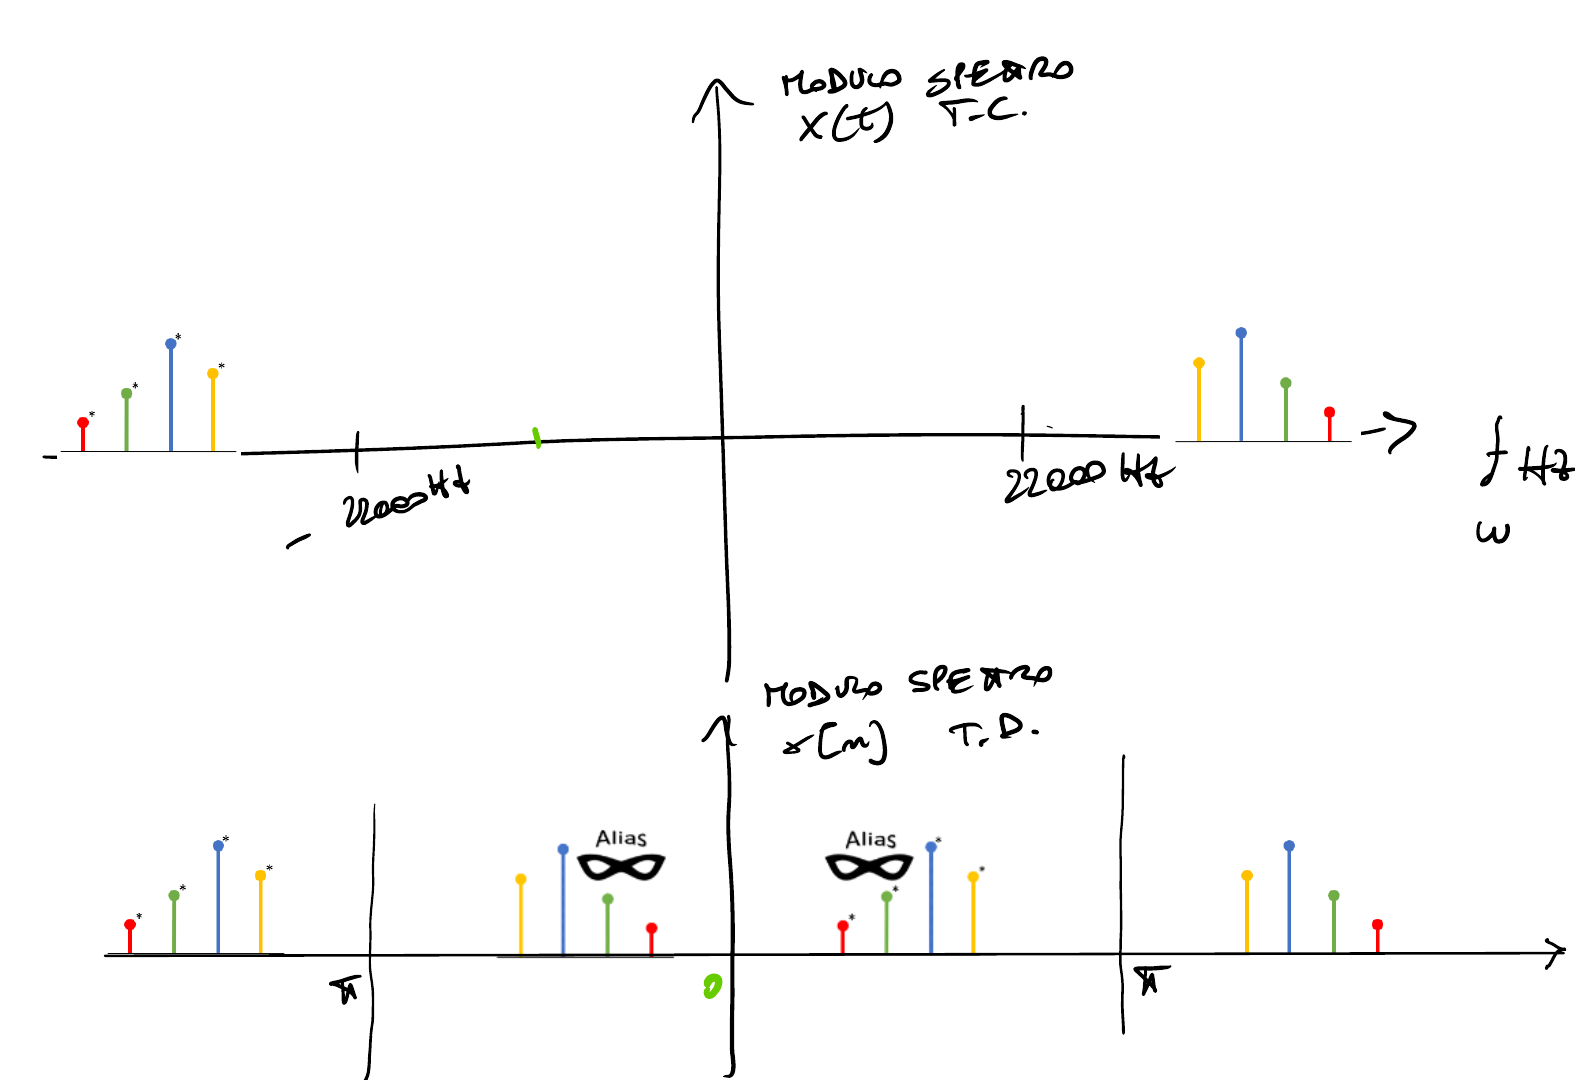
\includegraphics[scale=0.35]{immagini/lez11/spettroAlias.jpg}
\end{figure}

Quando campioniamo un segnale non rispettando il teorema di Shannon succede che le frequenze superano l'alias principale e di conseguenza vengono ribaltate creando rumore entrando nell'alias principale.

\section{Teorema del campionamento (Shannon)}
Dato un segnale tempo continui $x(t)$ a \textbf{banda limitata} B, lo si puo' ricostruire perfettamente dai propri campioni se e solo se

\[
    f_s = 2B
\]

Utilizzando un \underline{kernel di ricostruzione} ottimo

\[
    p(t)= \frac{\sin(\frac{\pi t}{T_s})}{\frac{\pi t}{T_s}} = sinc(\pi t f_s)
\]

Con banda limitata intendiamo un segnale composto da tante cosinusoidi ma che non vanno all'infinito, di conseguenza ne esiste una massima, quindi e' la frequenza massima appartenente ad un segnale. 

\begin{figure}[ht!]
    \centering
    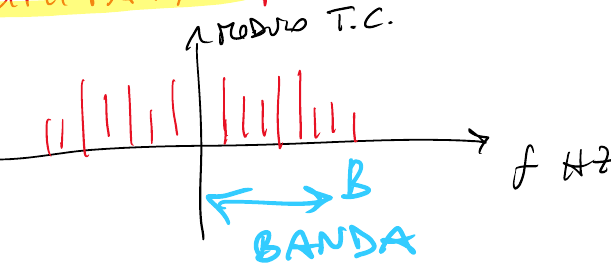
\includegraphics[scale=0.35]{immagini/lez10/banda.jpg}
\end{figure}

Diamo adesso della terminologia:
\begin{itemize}
    \item NYQUIST RATE: e' il doppio della frequenza massima $2B, 2F_{MAX}$. Noi dobbiamo sempre campionare usando una $f_s >$ della NYQUIST RATE.
    \item NYQUIST FREQUENCY: e' la meta' della frequenza di campionamento $\frac{f_s}{2}$.
\end{itemize}

\subsection{Ricostruire un segnale}
Ma effettivamente cosa vuol dire ricostruire un segnale? 
Se vogliamo capire la seconda parte del teorema di Shannon dobbiamo capire cosa si intende con kernel di ricostruzione.
Partiamo ripassando cosa significa interpolazione in linguaggio matematico. Significa trovare una funzione che passa da certi punti. Esistono molti modi di fare un'interpolazione, ad esempio lineare (colleghiamo linearmente due punti).
Nell'esempio in figura vediamo due tipi di interpolazione dati tre punti:

\begin{figure}[ht!]
    \centering
    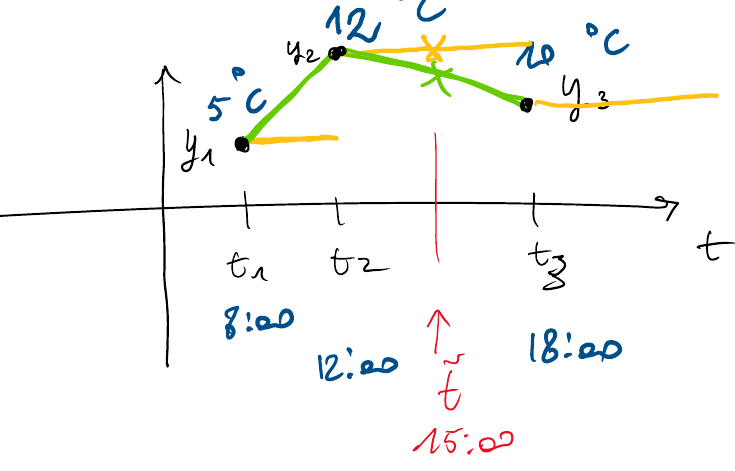
\includegraphics[scale=0.2]{immagini/lez10/interpolazione.jpg}
\end{figure}



Ricostruire un segnale e' come fare un interpolazione, abbiamo dei campioni e dobbiamo "collegare" i vari campioni per ricostruire un segnale quanto piu' possibile fedele all'originale.

Abbiamo vari modi di fare la ricostruzione, ad esempio esiste la ricostruzione di \underline{ordine zero (Z.0.H)}, in cui decido che il segnale negli intervalli e' costante. 
Il Kernel di ricostruzione in questo caso e' il rettangolo di altezza 1 in basso in figura, che e' come se prendessi e mettessi centrato per ogni campione e lo uso per ricostruire il segnale.

\begin{figure}[ht!]
    \centering
    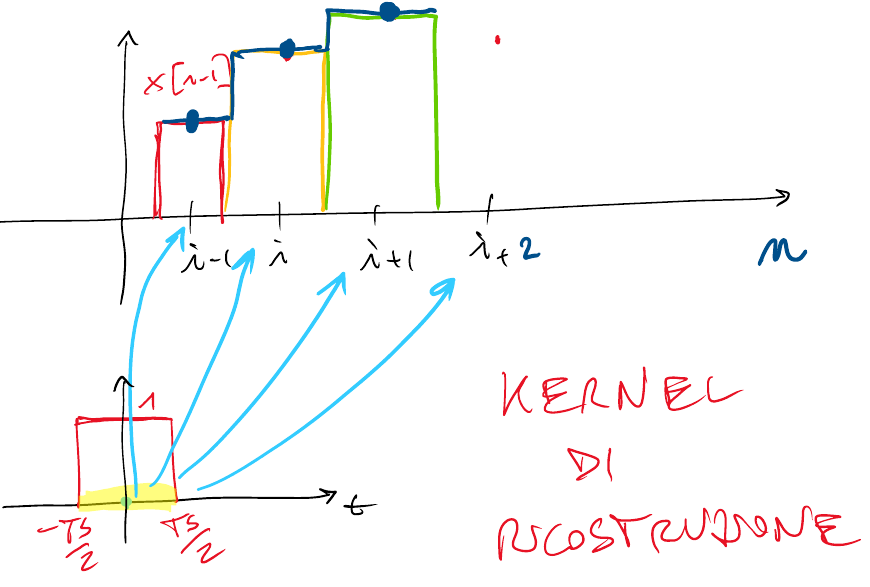
\includegraphics[scale=0.35]{immagini/lez10/ordineZero.jpg}
\end{figure}

Potremmo fare anche una ricostruzione lineare di primo grado, ovvero tracciamo una retta tra i vari campioni. In questo caso il kernel di ricostruzione e' un triangolo con base $-T, T$ ed alto 1, che prendiamo e posizioniamo su ogni campione, e sommiamo tutti i triangoli. Ovviamente come si nota dal grafico ci sono delle sovrapposizioni tra i trinagoli:

\begin{figure}[ht!]
    \centering
    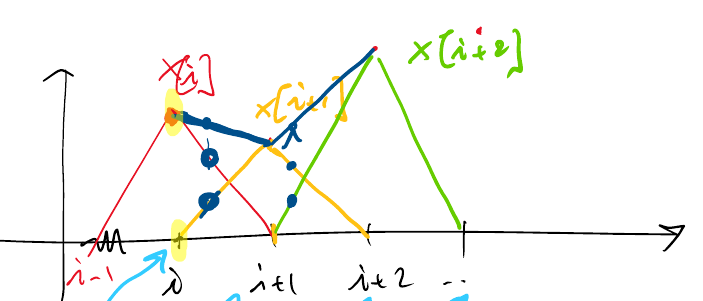
\includegraphics[scale=0.35]{immagini/lez10/lineare.jpg}
\end{figure}

\medskip
\medskip
\medskip
\medskip
\medskip
\medskip
\medskip
\medskip
\medskip
\medskip
\medskip
\medskip
\medskip
\medskip
\medskip
\medskip
\medskip
\medskip


\subsubsection{Dimostrazione ricostruzione lineare}
Dimostriamo che effettivamente la ricostruzione lineare funziona.
Inizialmente abbiamo un grafico in cui sono presenti due punti:

\begin{figure}[ht!]
    \centering
    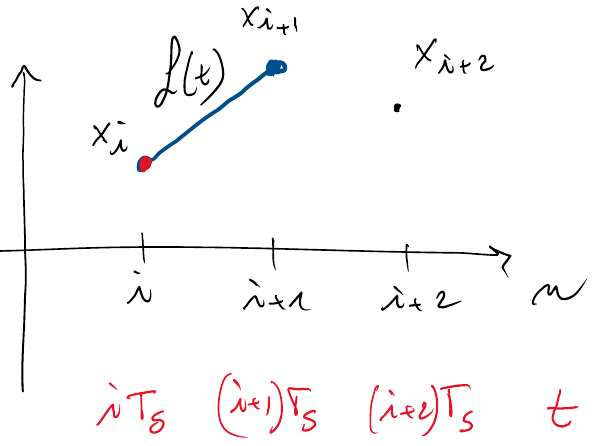
\includegraphics[scale=0.35]{immagini/lez10/linearePartenza.jpg}
\end{figure}

noi dato che stiamo ricostruendo linearmente dobbiamo tracciare una linea retta tra i due punti, e quello che otteniamo la chiamiamo $f(t)$, che e' l'equazione della retta che passa dai due punti:

\[
    f(t) = (t-i T_s) \frac{x_{i+1} - x_i}{(i + 1)T_s - i T_s} + x_i
\]

Facciamo due verifiche per capire che l'equazione e' corretta:

\[\begin{split}
    f(i T_s) &= (i T_s - i T_s) \frac{x_{i+1} - x_i}{(i+1)T_s - i T_s} + x_1 = x_i \\
    f((i + 1)T_s) &= ((i+1)T_s - i T_s) \frac{x_{i+1} - x_i}{(i + 1) T_s - i T_s} + x_i = x_{i+1}
\end{split}\]

Verificato che l'equazione passa effettivamente per quei punti, portiamo tutti i termini (dell'equazione della retta) che dipendono da $x_i$ a sinistra e tutti quelli che dipendono da $x_{i+1}$ a destra:

\[
    x(t) = -\frac{x_i}{T_s} (t - i T_s) + x_i +\frac{x_{i+1}}{T_s} (t - i T_s)
\]

E notiamo che la parte sinistra dell'equazione e' la retta che parte dal punto $x_i$ ed arriva a $i+1$, mentre la parte di destra e' la retta che parte da $x_{i+1}$ ed arriva ad $i$. Quindi la retta che passa tra i due punti e' la somma dei segmenti ottenuti precedentemente. 
E se ripetiamo questo procedimento utilizzando la parte sinistra per il punto $x_{i+1}$ e la parte destra per il punto $x_i$, notiamo che si ottiene un triangolo, che e' il kernel di ricostruzione.

\begin{figure}[ht!]
    \centering
    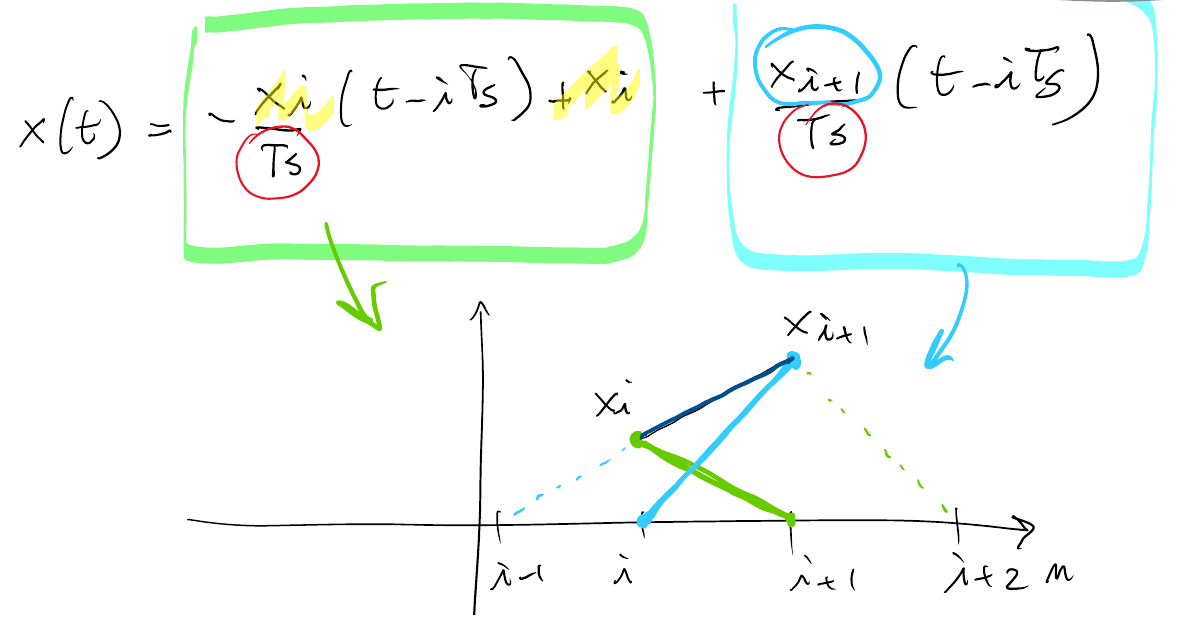
\includegraphics[scale=0.35]{immagini/lez10/lineareDimostrazione.jpg}
\end{figure}

\subsection{Funzionamento kernel ottimo}
Il kernel di interpolazione ottimo previsto da Shannon ricordiamo essere:

\[\begin{split}
     P(t)=
    \begin{cases}
    \frac{\sin \pi t F_s}{\pi t F_s} \text{ se } t \ne 0 \\
    1 \text{ se } t = 0 \\
    \end{cases}
    = sinc \pi t F_s
\end{split}
\]

\begin{figure}[ht!]
    \centering
    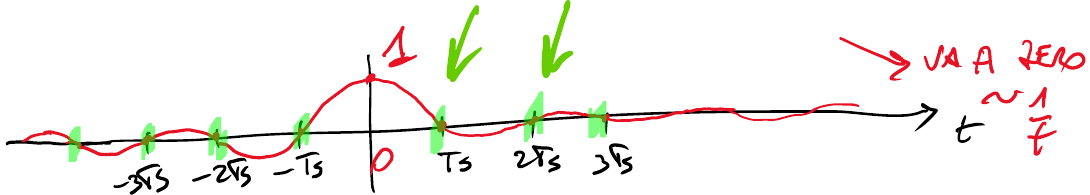
\includegraphics[scale=0.35]{immagini/lez12/kernelOttimo.jpg}
\end{figure}

Ma come funziona? E' una funzione che oscilla da meno a piu' infinito, pari e si rastrema all'infinito come $\frac{1}{T}$, come un iperbole, che va a zero lentamente. Inoltre passa per zero tutte le volte che $\pi t f_s = k \pi, k \in \mathbf{Z}$, ovvero $t = \frac{1}{f_s} k = k \cdot T_s$.
E' zero in tutti i campioni (dove passa la griglia di campionamento) eccetto lo zero, dove vale 1.
Quello che dobbiamo fare e' prendere questo kernel e giustapporrlo ad ogni campione e poi sommarli.

Esempio:

\begin{figure}[ht!]
    \centering
    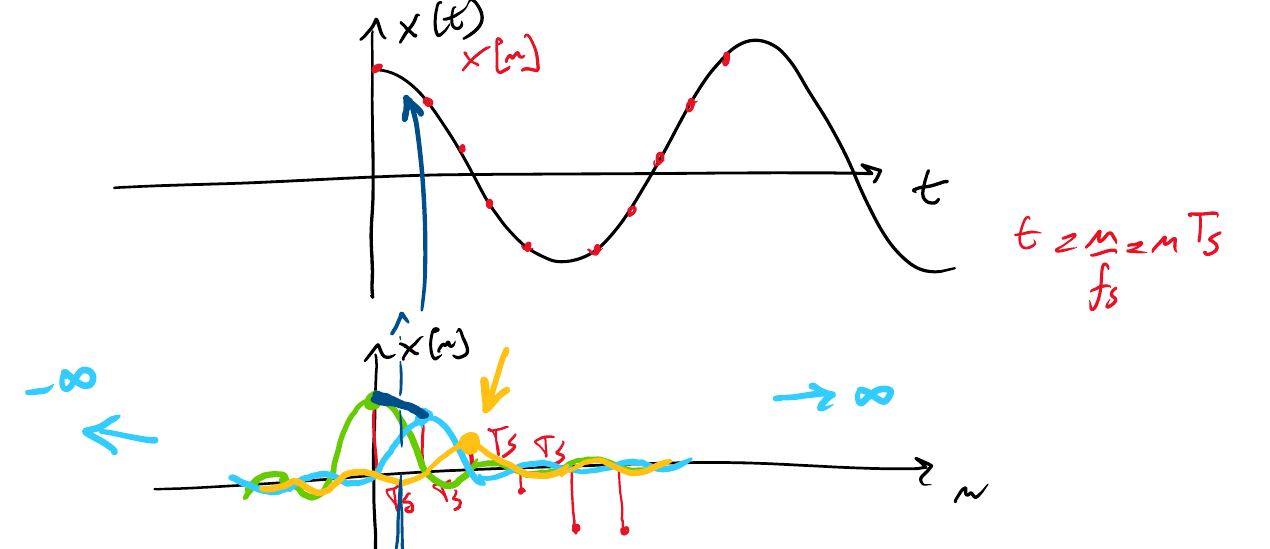
\includegraphics[scale=0.35]{immagini/lez12/usoKernelOttimo.jpg}
\end{figure}

dobbiamo prendere il kernel di ricostruzione e modularlo su ogni punto, non possiamo fermarci da $-T_s, T_s$ ma va fatto per tutti i campioni, fino ad infinito.

Ma dato che nella realta' abbiamo un numero di campioni finito lo possiamo usare.
Ora ipotizzando una canzone di 4 minuti ed ipotizzando di campionarla a 44100 campioni al secondo (che e' quello che si fa nella realta'), per ricostruire perfettamente il segnale dovremmo avere 10584000 kernel. Quindi capiamo che per un problema di prestazioni raramente si usa questo kernel per ricostruire i segnali, ma ci accontentiamo del fatto che un segnale rispetti il teorema di Shannon e poi usiamo un kernel piu' facile (ad esempio lineare, 0, quadratico).

\chapter{Sistemi}
Dopo aver parlato di segnali a tempo continuo e segnali a tempo discreto, il nostro obbiettivo ora e' scrivere un algoritmo per modificare un segnale. In generale questa operazione sara' fatta costruendo dei filtri (o SISTEMI) che hanno in ingresso un segnale a tempo discreto ed in uscita sempre un segnale a tempo discreto.

\section{Esempio di sistemi, equazione alle differenze}
Troviamo un modo matematico per esprimere gli algoritmi.
Un operatore matematico che si applica ad un segnale tempo discreto e' detto \textbf{equazione alle differenze}, il quale ha in uscita un segnale tempo discreto ed in uscita sempre un segnale a tempo discreto.

Vediamo ora degli esempi di sistemi. Innanzitutto diamo delle definizioni, chiameremo n (la variabile indipendente) \textbf{presente}, di conseguenza considereremo un segnale con in input solo n, input presente.
Mentre considereremo un segnale $x[n - k], k \in \mathbf{N}$, \textbf{input passato}, invece un segnale $x[n + k], k \in \mathbf{N}$, \textbf{input futuro}. $y[n]$ e' considerato l'\textbf{output}

\[\begin{split}
    y[n] &= (x[n])^2 \\
    y[n] &= (x[n])^3 - x[n-1] + \frac{1}{2} x[n+1]
\end{split}\]

\section{Proprieta' dei sistemi}
\begin{itemize}
    \item Causale: sistema che dipende dal presente e dal passato: $y[n] = x[n-1]$
    \item Anti-Causale: sistema che dipende dal futuro $y[n] = x[n+2]$
    \item A-Causali: sistema che dipende sia dal passato che dal futuro: $y[n] = \frac{x[n+1] - x[n-1]}{2}$
\end{itemize}

\begin{figure}[ht!]
    \centering
    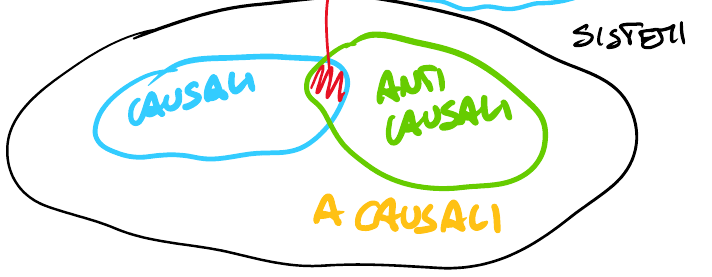
\includegraphics[scale=0.35]{immagini/lez12/sistemi.jpg}
\end{figure}

\section{Definizione di segnali tempo discreti particolari}
Diamo ora delle definizioni di segnali particolari che ci serviranno successivamente.

\subsection{Delta di Kronecker (impulso discreto)}
E' un segnale che vale 1 nel punto 0 e 0 in tutti gli altri punti. Ha quindi la caratteristica di essere estremamente collocato nel tempo.

\[\begin{split}
    \delta[n] = 
    \begin{cases}
    1 \text{ se } n = 0 \\
    0 \text{ se } n \ne 0 \\
    \end{cases}
\end{split}\]

Equivale alla modellazione discreta di un evento ad impulsi, ad esempio lo scoppio di un palloncino.

\begin{figure}[ht!]
    \centering
    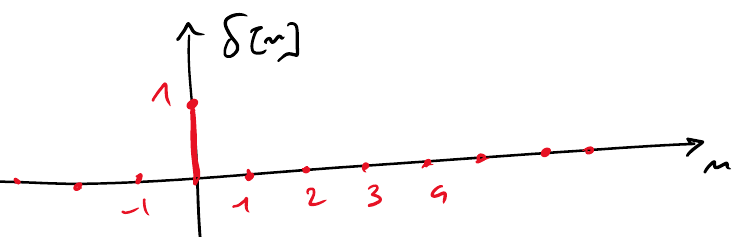
\includegraphics[scale=0.35]{immagini/lez12/delta.jpg}
\end{figure}

\subsection{Gradino causale (step function)}

\[\begin{split}
    u[n] = 
    \begin{cases}
    1 \text{ se } n \le 0 \\
    0 \text{ se } n < 0 \\
    \end{cases}
\end{split}\]

Possiamo considerarlo come un segnale che si attiva in un certo istante e poi rimane attivo all'infinito.

\begin{figure}[ht!]
    \centering
    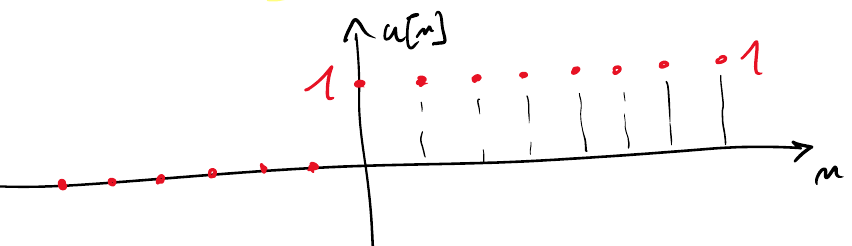
\includegraphics[scale=0.35]{immagini/lez12/gradinoCausale.jpg}
\end{figure}

\subsection{Gradino anticausale}
E' l'opposto del gradino causale:

\[\begin{split}
    -u[-n-1] = 
    \begin{cases}
    0 \text{ se } n \ge 0 \\
    -1 \text{ se } n < 0 (n \le 1) \\
    \end{cases}
\end{split}\]

Possiamo considerarlo come un segnale che esisteva da meno infinito in passato ed ad un certo punto finisce.

\begin{figure}[ht!]
    \centering
    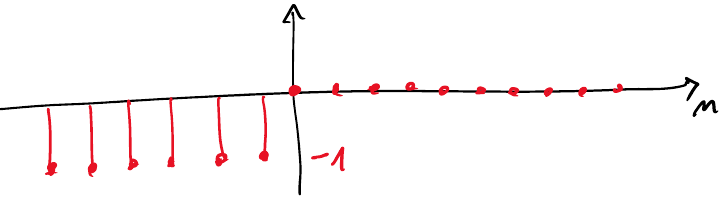
\includegraphics[scale=0.35]{immagini/lez12/gradinoAnticausale.jpg}
\end{figure}

\section{Altre poprieta' dei sistemi}

\subsection{Tempo-Invarianza (invarianza temporale)}

E' un concetto che possiamo facilmente ricondurre alla realta', noi ci aspettiamo sempre che se rifacciamo un'azione a distanza di tempo l'output derivato da quell'azione e' lo stesso, ad esempio riprodurre la stessa canzone una volta la mattina ed una la sera, ci aspettiamo che la canzone riprodotta sia la medesima.

Nell'esempio vediamo che se ritardiamo l'input di $n_0$ campioni, allora anche l'output e' ritardato degli stessi campioni $n_0$.

Vediamo ora degli esempi di tempo invarianza, vediamo come nel primo esempio, avendo un segnale tempo invariante (non dipendente da n), nonostante applichiamo un ritardo, all'ingresso o all'uscita del sistema, l'output non cambia. 
Mentre nel secondo caso il sistema $nx[n]$ e' strettamente dipendente ( dalla n che moltiplica il sistema) notiamo che gli outpu applicando il ritardo prima o dopo il sistema cambiano, quindi non e' tempo invariante. Generalizzando possiamo dire che un segnale che dipende strettamente dal tempo non e' a tempo invariante.

\begin{figure}[ht!]
    \centering
    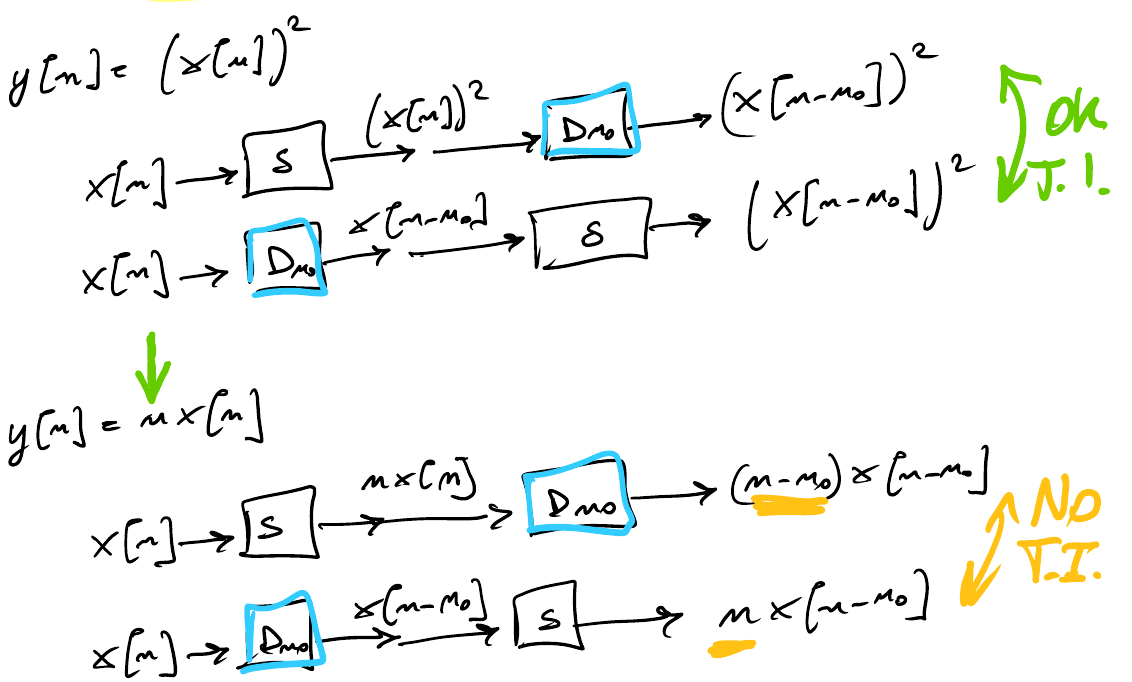
\includegraphics[scale=0.35]{immagini/lez12/esTempoInvarianza.jpg}
\end{figure}

Vedendolo in modo piu' "informatico" possiamo considerare il ritardo come se spostassimo di $n_0$ posizioni un array.

\begin{figure}[ht!]
    \centering
    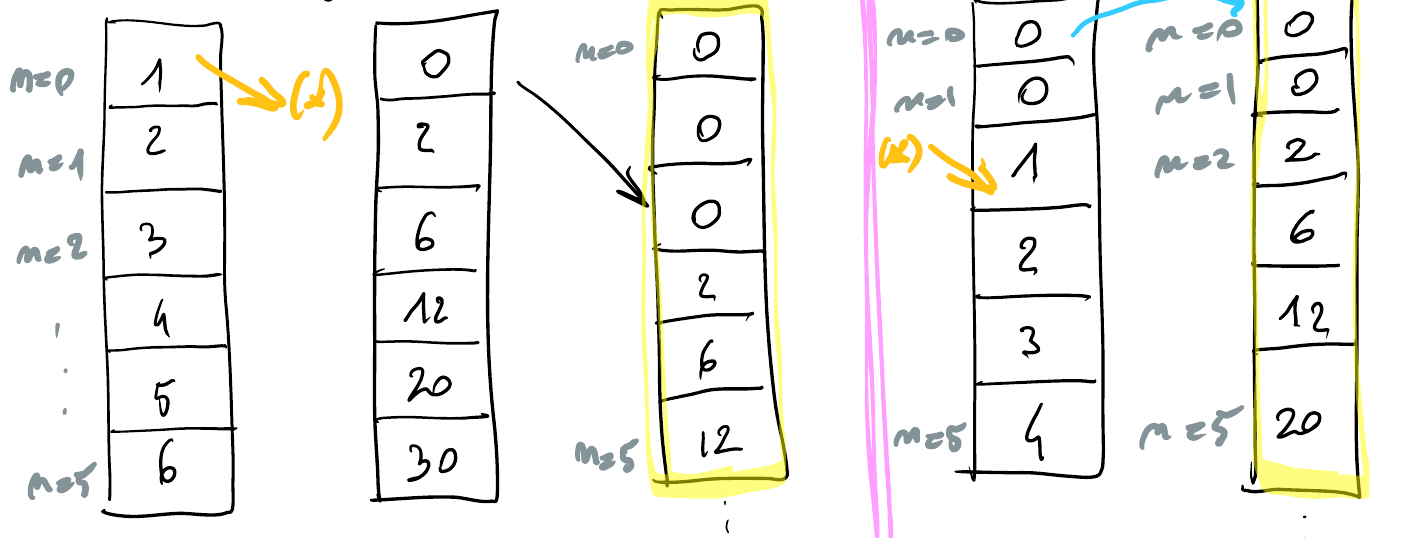
\includegraphics[scale=0.35]{immagini/lez12/tempoInvarianzaArray.jpg}
\end{figure}

\subsection{Linearita'}
Avendo un sistema con 2 input $x_1[n], x_2[n]$ e registro gli output del sistema $y_1[n], y_2[n]$, se invece mettiamo in input delle combinazioni lineari degli intput: $\alpha x_1[n], \beta x_2[n]$, ci sara' ancora una relazione con gli input precedenti?
Si se il sistema e' lineare, ed otterremo una combinazione lineare degli ouput di prima con gli stessi coeficienti degli input :$\alpha y_1[n], \beta y_2[n]$

\begin{figure}[ht!]
    \centering
    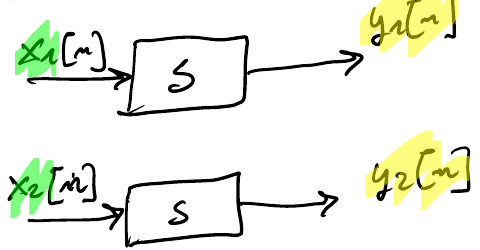
\includegraphics[scale=0.35]{immagini/lez12/linearita.jpg}
\end{figure}

Quello che facciamo in pratica e' dare degli stimoli al sistema e vederne gli effetti.

\section{Di che sistemi trattiamo}
In questo corso tratteremo solo di segnali lineare e tempo invarianti (LTI).

\begin{figure}[ht!]
    \centering
    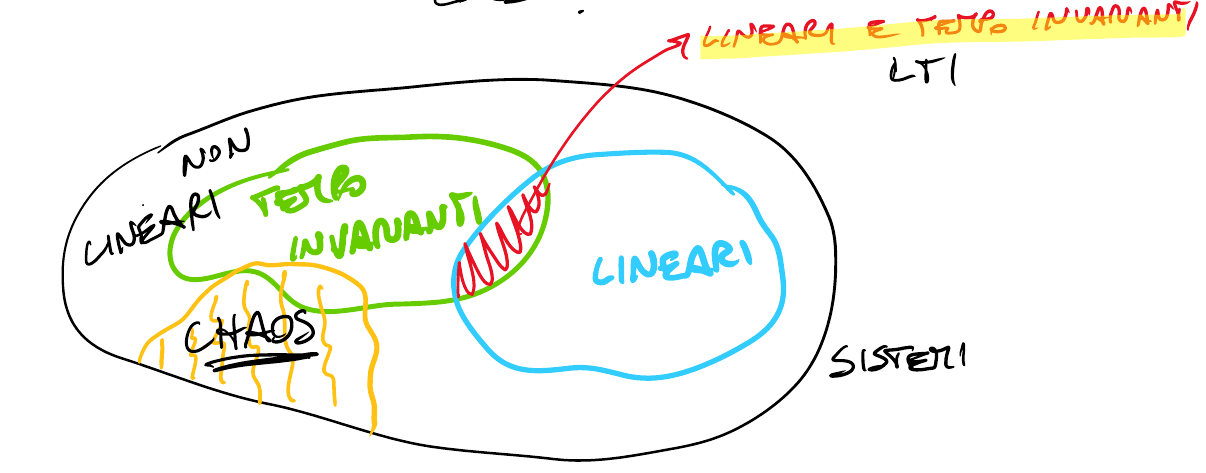
\includegraphics[scale=0.35]{immagini/lez12/sistemiTrattiamo.jpg}
\end{figure}

Notiamo che ci sono dei sistemi che godono della proprieta' del CHAOS, ovvero hanno estrema dipendente dalle condizioni iniziali.

\subsection{Esempio}
Prendiamo un input e lo mettiamo in un sistema.

In questo esempio useremo una delta nel sistema e notiamo che in uscita dal sistema abbiamo ancora una delta. Quello che facciamo quindi e' aver calcolato la \textbf{risposta del sistema} quando l'ingresso e' un impulso discreto, \textbf{risposta all'impulso}.

\[\begin{split}
    y[n] &= (x[n])^2 \\
    x[n] &= \delta[n] \\
    y[n] &= (\delta[n])^2 = \delta[n]
\end{split}\]

\begin{figure}[ht!]
    \centering
    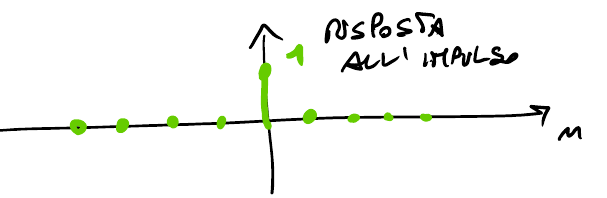
\includegraphics[scale=0.35]{immagini/lez12/esA.jpg}
\end{figure}

Ora cambiamo il sistema (sempre lineare e tempo invariante, LTI), e ci mettiamo sempre in input la delta e calcoliamo la risposta del sistema:

\[\begin{split}
    y[n] &= \frac{1}{2} x[n] + \frac{1}{2} x[n-1] \\
    x[n] &= \delta[n] \\
    y[n] &= h[n] = \frac{1}{2} \delta[n] + \frac{1}{2} \delta[n-1]
\end{split}\]

Per disegnare il grafico del segnale, notando che e' la somma di due funzioni delta, prendiamo la prima la dividiamo per 2, ovvero dove valeva 1 ora vale $\frac{1}{2}$ e dove valeva 0 rimane a 0, alla quale sommo un'altra funzione delta anch'essa divisa per 2 e traslata verso destra di 1 (perche' come sappiamo sottrarre un numero dalla variabile dipendente della funzione significa traslare verso destra la funzione del valore sottratto).

\begin{figure}[ht!]
    \centering
    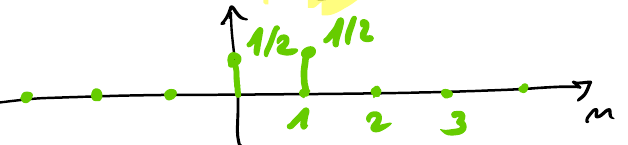
\includegraphics[scale=0.35]{immagini/lez12/esB.jpg}
\end{figure}

\section{Scomposizione con delta traslate}
Osserviamo che qualunque segnale puo' essere scomposto come somma di impulsi opportunamente scalati e traslati.

Disegniamo un segnale qualunque $x[n]$ che ha un supporto compatto, ovvero ha un dominio limitato nel tempo (e' definito nel tempo in un certo intervallo). Notiamo che ogni campione del segnale puo' essere scritto come una funzione delta scalata di un valore (l'altezza y) e traslata sull'asse x.

\begin{figure}[ht!]
    \centering
    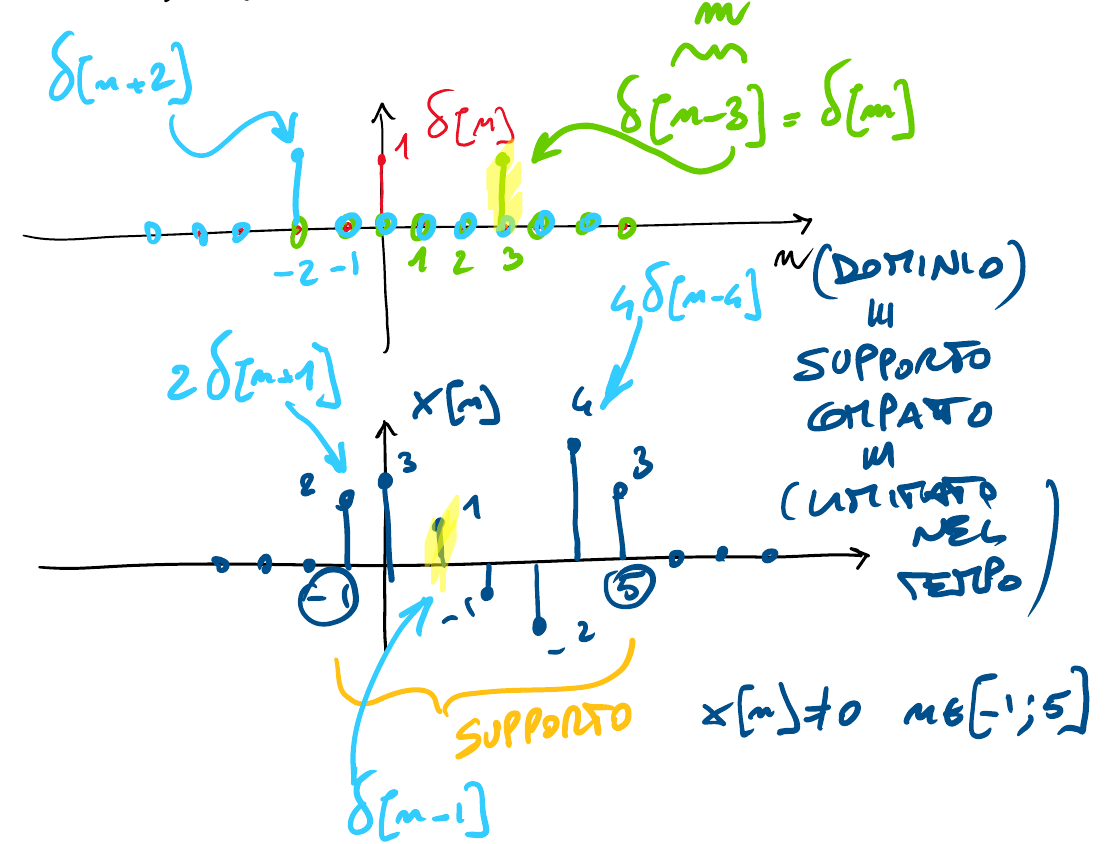
\includegraphics[scale=0.35]{immagini/lez13/composizioneDelta.jpg}
\end{figure}

Riscriviamo quindi il segnale come composizione di delta:
\[
    x[n] = 2 \delta[n+1] + 3 \delta[n] + \delta[n-1] - \delta[n-2] -2 \delta[n-3] + 4 \delta[n-4] + 3 \delta[n-5]
\]

Questa cosa possiamo farla con qualsiasi segnale:

\[
    x[n] = \sum_{k = - \infty}^{+\infty} x[k] \delta[n-k]
\]

dove $x[n]$ e' il valore del segnale nel punto (la modulazione delle y), $\delta[n-k$ e' la funzione delta traslata nel tempo. Inoltre notiamo che generalizzando si puo' scomporre un segnale anche che non abbia un supporto compatto.

Ci serve per descrivere in modo naturale un segnale, un insieme di campioni nel tempo con valori diversi.

\section{Prodotto di convoluzione}
Vediamo che la risposta all'impulso (che esiste sempre) per i sistemi lineari e tempo invarianti ci permette di descrivere le uscite dal sistema per qualunque segnale.

Consideriamo quindi un sistema generale, con input $x[n]$ ed output $y[n]$. Possiamo scrivere $y[n]$ come composizione lineare degli $x[n]$, inoltre posso anche sostituire al segnale $x[n]$ la sommatoria di funzione delta (come abbiamo appena visto), ottenendo:

\[
    y[n] = L(\sum_{k = - \infty}^{+ \infty} x[k] \delta[n-k])
\]

quindi possiamo usare la linearita' dell'operatore lineare L, dato che $x[n]$ e' un numero:

\[
    y[n] =\sum_{k = - \infty}^{+ \infty} x[k] L(\delta[n-k])
\]

il nostro sistema e' anche tempo invariante, abbiamo spostato l'input ($\delta[n-k]$), quindi mi aspetto che anche l'output sia spostato nel tempo ($h[n-k]$).

\begin{figure}[ht!]
    \centering
    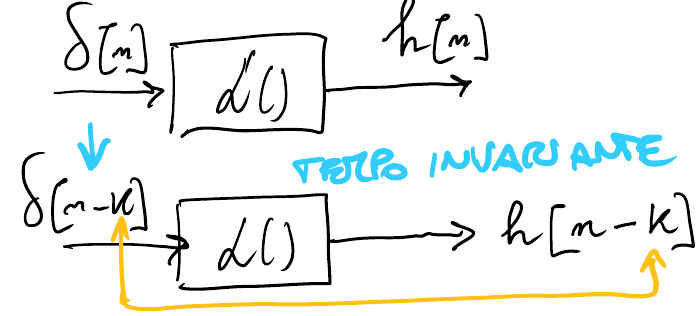
\includegraphics[scale=0.35]{immagini/lez13/tempoInvarianteConvoluzione.jpg}
\end{figure}

\[
    y[n] =\sum_{k = - \infty}^{+ \infty} x[k] h[n-k]
\]

Quindi se conosciamo $h[n]$ possiamo calcolare $y[n]$ qualsiasi sia l'input. La risposta all'inpulso caratterizza perfettamente il mio sistema.
L'operazione si chiama prodotto di convoluzione:

\[
    \sum_{k = - \infty}^{+ \infty} x[k] h[n-k] = x[n] * h[n]
\]

\subsection{Proprieta' del prodotto di convoluzione}

\subsubsection{Commutativa}
\[\begin{split}
    y[n] &= x[n] * h[n] = \sum_{k = - \infty}^{+ \infty} x[k] h[n-k] \\
    y[n] &= h[n] * x[n] = \sum_{k = - \infty}^{+ \infty} h[k] x[n-k]
\end{split}\]

\subsubsection{Associativa}
\[\begin{split}
    (x[n] * y[n]) * z[n] = x[n] * (y[n] * z[n])
\end{split}\]

\subsubsection{Distributiva rispetto alla somma}
\[\begin{split}
    (x[n] + y[n]) * z[n] = x[n] * z[n] + y[n] * z[n]
\end{split}\]

\subsubsection{Elemento neutro}
\[\begin{split}
    x[n] * e[n] &= x[n] \\
    e[n] &= \delta[n] \\
    x[n] * \delta[n] &= \sum_{k = - \infty}^{+ \infty} x[k] \delta[n-k] = x[n]
\end{split}\]

\subsection{Razionalizzando la convoluzione}

Riscriviamo la convoluzione ribaltando e la traslazione nel tempo:

\[
    \sum_{k = - \infty}^{+ \infty} x[k] h[n-k] = h[-(k-n)]
\]

\section{Risposta in frequenza}

\begin{figure}[ht!]
    \centering
    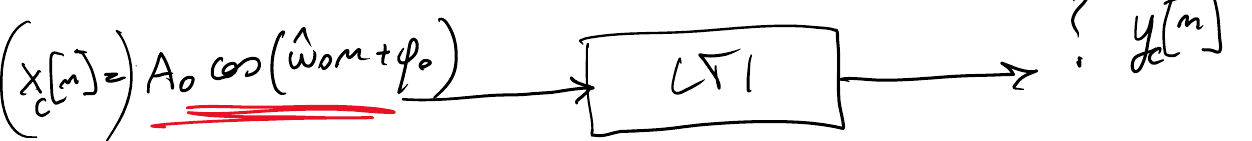
\includegraphics[scale=0.35]{immagini/lez13/cosinusoideDiscreta.jpg}
\end{figure}

Possiamo scomporre con Eulero la cosinusoide:

\[\begin{split}
    \sum_{k = -\infty}^{+\infty} \frac{A_0}{2} \{ e^{\hat{\omega_0} k i} e^{i \varphi_0} + e^{- \hat{\omega_0} k i} e^{- i \varphi_0} \} h[n-k]\\
    \mbox{Separiamo la sommatoria sulla somma} \\
    \sum_{k = -\infty}^{+\infty} \frac{A_0}{2} \{ e^{\hat{\omega_0} k i} e^{i \varphi_0} h[n-k] \} + &\sum_{k = -\infty}^{+\infty} \frac{A_0}{2} \{ e^{- \hat{\omega_0} k i} e^{- i \varphi_0} h[n-k] \} \\
    \mbox{Portiamo fuori i termini costanti che non dipendono da k} \\
    \frac{A_0}{2} e^{i \varphi_0} \cdot \sum_{k = -\infty}^{k = +\infty} e^{+i \hat{\omega_0}k} h[n-k] + \frac{A_0}{2} e^{-i \varphi_0} \cdot \sum_{k = -\infty}^{k = +\infty} e^{-i \hat{\omega_0}k} h[n-k] \\
    \mbox{Notiamo che ci sono termini che sono complessi e complessi coniugati} \\
    \mbox{Applichiamo ora la proprieta' commutativa della convoluzione} \\
    \frac{A_0}{2} e^{i \varphi_0} \cdot \sum_{k = -\infty}^{k = +\infty} e^{+i \hat{\omega_0}(n-k)} h[k] + \frac{A_0}{2} e^{-i \varphi_0} \cdot \sum_{k = -\infty}^{k = +\infty} e^{-i \hat{\omega_0}(n-k)} h[k] \\
    \mbox{Posso applicare le proprieta' delle potenze} \\
    e^{\hat{\omega_0}(n-k)i} = e^{\hat{\omega_0} n i} e^{-\hat{\omega_0} k i} \\
    \mbox{Porto fuori i termini che non dipendono da k} \\
    \frac{A_0}{2} e^{i \varphi_0} e^{\hat{\omega_0}n i} \cdot \sum_{k = -\infty}^{k = +\infty} e^{-\hat{\omega_0}k i} h[k] + \frac{A_0}{2} e^{-i \varphi_0} e^{-\hat{\omega_0} n i} \cdot \sum_{k = -\infty}^{k = +\infty} e^{\hat{\omega_0} k i} h[k] \\
\end{split}\]

Arrivati a questo punto notiamo che $\sum_{k = -\infty}^{k = +\infty} e^{-\hat{\omega_0}k i} h[k]$ e' un numero complesso ed e' importante, quindi lo chiamiamo $H(e^{j \hat{\omega_0}})$ che dipende da $\hat{\omega_0}$, l'altro e' il complesso coniugato: $H^*(e^{j \hat{\omega_0}})$.

L'output di un sistema $y[n]$ quando abbiamo in input una cosinusoide discreta:

\[
y[n] = H(e^{j \hat{\omega_0}}) \frac{A_0}{2} e^{i \varphi_0} e^{\hat{\omega_0}n i} + H^*(e^{j \hat{\omega_0}}) \frac{A_0}{2} e^{-i \varphi_0} e^{-\hat{\omega_0} n i}
\]

Ora riscriviamo i termini in H in forma polare (ricordando che la parte tra il modulo e' il modulo e l'esponenziale moltiplicato per il modulo e' la fase):

\[\begin{split}
    y_c[n] &= | H(e^{j \hat{\omega_0}}) | e^{i \varphi H(e^{j \hat{\omega_0}})} \cdot \frac{A_0}{2} e^{i \varphi_0} e^{\hat{\omega_0}n i} + | H(e^{j \hat{\omega_0}}) | e^{-i \varphi H(e^{j \hat{\omega_0}})} \cdot \frac{A_0}{2} e^{-i \varphi_0} e^{-\hat{\omega_0}n i} \\
    &\mbox{Raccolgo i termini con la stessa base} \\
    &= | H(e^{j \hat{\omega_0}}) | \frac{A_0}{2} e^{i[\hat{\omega_0} n + \varepsilon_0 + \varphi H (e^{j \hat{\omega_0}})]} + | H(e^{j \hat{\omega_0}}) | \frac{A_0}{2} e^{-i[\hat{\omega_0} n + \varepsilon_0 + \varphi H (e^{j \hat{\omega_0}})]} \\
    y_c[n] &= | H(e^{j \hat{\omega_0}} | A_0 \cos [ \hat{\omega_0} n + \varepsilon_0 + \varphi_0 H (e^{j \hat{\omega_0}})]
\end{split}\]

Concludendo notiamo che in output dal sistema abbiamo un coseno con la stesse frequenza discreta di qu
ello messo in input.
Si dice quindi che il coseno e' un autofunzione di un sistema LTI, ovvero che non viene modificata nella sua forma funzionale (ha la stessa frequenza), ma al massimo iene traslato in ampiezza e fase.

$H(e^{i \hat{\omega_0}})$ e' detta \textbf{risposta in frequenza del sistema} $\in \mathbf{C}$.

\[
    H(e^{i \hat{\omega_0}}) = \sum_{k = -\infty}^{+\infty} h[n] e^{-i \hat{\omega_0} k }
\]

Approfondiamo ora le proprieta' della risposta in frequenza.

\subsection{Chiarimento}
Notiamo che abbiamo scritto la risposta in frequenza come una funzione $H(e^{j \hat{\omega}})$ che quindi non dipende da una singola variabile ma da un esponenziale, questo perche':

\[
  H(e^{j \hat{\omega}}) = \sum_{n = - \infty}^{+\infty} h[n] e^{-j \hat{\omega} n} =  \sum_{n = - \infty}^{+\infty} h[n] e^{(j \hat{\omega})-n} 
\]

Notiamo quindi che e' una funzione del termine $e^{i \hat{\omega}}$.
Inoltre specifichiamo utilizzando Eulero $e^{i \hat{\omega}} = \cos \hat{\omega} + i \sin \hat{\omega}$, dato che compare nella risposta in frequenza anche quest'ultima e' quindi una funzione periodica di periodo $2\pi$.

\subsection{Simmetria coniugata}
Perche' abbiamo sia la risposta in frequenza sia la sua coniugata.
\[\begin{split}
    H(e^{j \hat{\omega}}) &= \{ H(e^{-j \hat{\omega}}) \}^* \\
    H(e^{j \hat{\omega}}) &= \sum_{n = - \infty}^{+ \infty} h[n] e^{-i \hat{\omega}n} \\
    H(e^{-j \hat{\omega}}) &= \sum_{n = - \infty}^{+ \infty} h[n] e^{-i (\hat{- \omega}) n} = \sum_{n = - \infty}^{+ \infty} h[n] e^{i \hat{\omega}n} \\
    (\sum_{n = - \infty}^{+ \infty} h[n] e^{i \hat{\omega}n})^* &= H(e^{j \hat{\omega}})
\end{split}\]

Quindi possiamo dire che la risposta in frequenza ha una parte reale che e' il mudolo che ha simmetria pari, ed una parte immaginaria che e' la fase con simmetria dispari.

\section{Supporto risposta all'impulso}
La risposta all'impulso si divide in due categorie:
\begin{itemize}
    \item FIR (Finite Impulse Response): se ho un supporto compatto allora si chiama risposta all'impulso finita, nel supporto e non nell'ampiezza (che e' finita di perse'). $h[n] \neq 0 \rightarrow n \in [a,b]$.
    \item IIR (Infinite Impulse Response): se non ha un supporto compatto si chiama risposta all'impulso infinita. $h[n] \neq 0 \rightarrow n < > a$
\end{itemize}

Abbiamo quindi una prima intuizione di filtro, in quanto la risposta all'impulso e' un filtro con cui calcoliamo l'uscita di un sistema.

\section{Equazione alle differenze di un qualunque sistema LTI}
Possiamo definire un'equazione alle differenze standard per qualunque sistema LTI:

\[
    y[n] = \sum_{h = -N_1, h \neq 0}^{N_2} a h y[n-h] + \sum_{k = -M_1}^{M_2} bk x[n-k]
\]

In cui $ah$ e $bk$ sono costanti, $y[n-h$ e' l'uscita del sistema futura o passata e $x[n-k]$ e' l'input del sistema (presente, passato o futuro).
La prima sommatoria si chiama parte \underline{AUTOREGRESSIVA (AR)} che dipende dall'output del sistema.
La seconda sommatoria si chiama \underline{MEDIA MOBILE (MA)} o MOUVING AVERAGE, che dipende solamente dall'input al sistema.
Se riusciamo a ricondurre l'equazione alle differenze di un sistema a questa equazione generale non dobbiamo verificarne la linearita' e la tempo invarianza.

Inoltre possiamo dire che condizione sufficiente (ma non necessaria) per un sistema LTI per avere risposta all'impulso finita (FIR) e' che $ah = 0, \forall h$. Vuol dire che non c'e' dipendenza dall'output ma solamente dall'input, ovvero non esiste la parte autoregressiva.

Notiamo inoltre che se e' presente la parte autoregressiva NON posso dire che il sistema non e' FIR.

\section{Filtraggio (pratico) con sistemi LTI}
Proviamo a capire perche' ci interessa la risposta all'impulso di un sistema.

\begin{figure}[ht!]
    \centering
    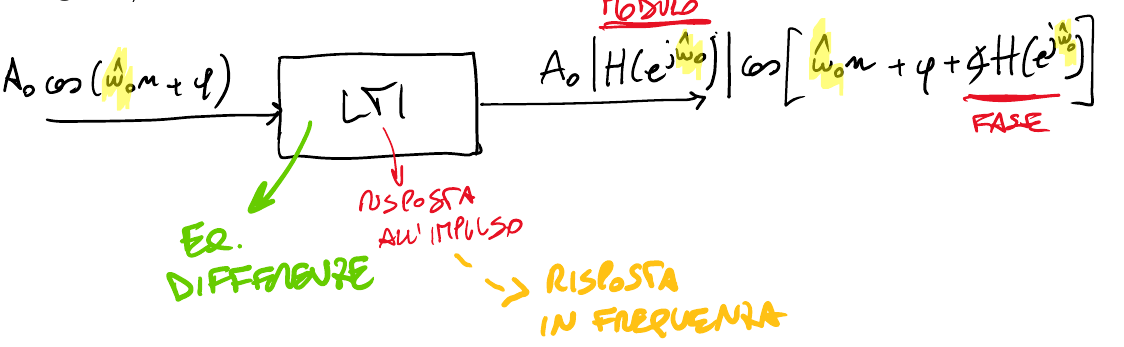
\includegraphics[scale=0.35]{immagini/lez15/uscitaLTIcoseno.jpg}
\end{figure}

Ricordiamo innanzitutto che l'uscita di sistema LTI quando l'input e' una cosinusoide discreta e' una cosinusoide discreta con la stessa frequenza ma modulata in modulo e fase.
Questa nozione e' alla base del filtraggio pratico con sistemi LTI.
Partiamo dall'ipotesi che abbiamo un segnale discreto da filtrare, che e' una combinazione lineare di cosinusoidi discrete. Quello che voglio fare e' fare agire il filtro tipo un setaccio, per far passare solo le cosinuosidi che mi interessano e scartare quelle che non mi interessano.
Notiamo che e' il modulo della risposta in frequenza che puo' fare questa operazione, in quanto se lo mettiamo uguale a 0 il coseno non esiste, quindi e' come se lo avessimo "bloccato".
Inoltre potremmo anche amplificare (o diminuire) l'ampiezza di una cosinusoide, se il modulo della risposta in frequenza fosse $\neq 0$.

Quindi il modulo della risposta in frequenza puo' aumentare o diminuire l'ampiezza (in verticale $\hat{|}$) della cosinusoide, mentre la fase ci permette di spostarla (in orizzontale $\leftrightarrow$) rispetto a quella che mettiamo in ingresso al sistema LTI.

\begin{figure}[ht!]
    \centering
    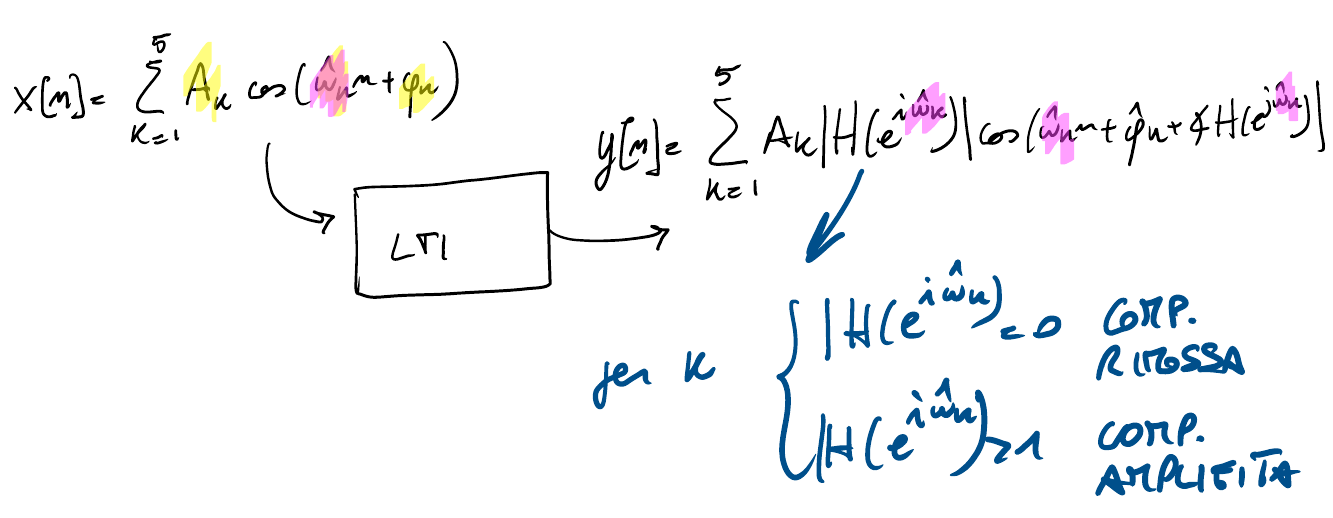
\includegraphics[scale=0.35]{immagini/lez15/filtraggioLTI.jpg}
\end{figure}

Sono stati definiti dei filtri ideali.

\subsection{Filtro passa basso (low pass)}
\begin{figure}[ht!]
    \centering
    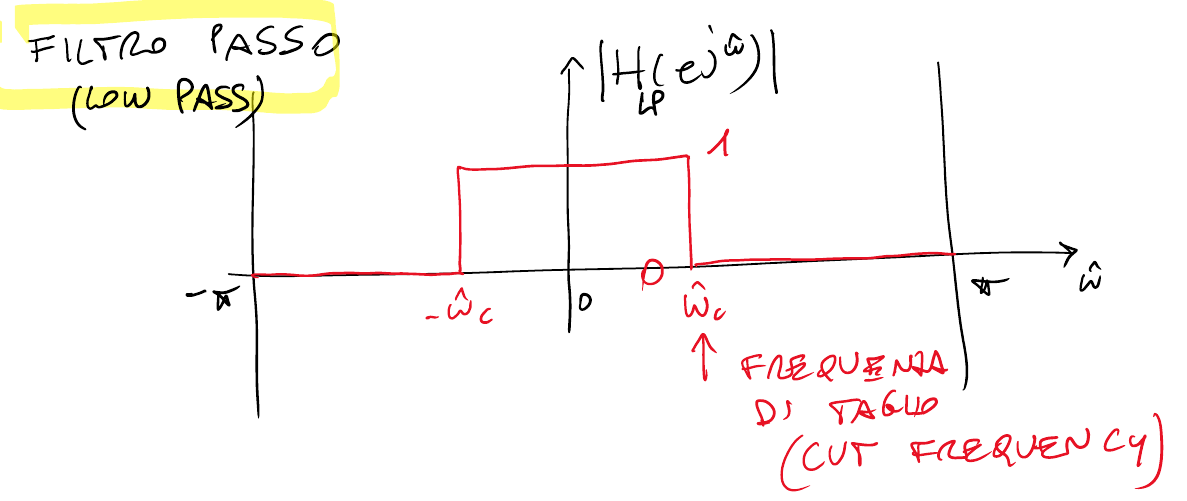
\includegraphics[scale=0.35]{immagini/lez15/passaBasso.jpg}
\end{figure}

Innanzitutto notiamo che il grafico del filtro e' rappresentato tra $-\pi, \pi$ questo perche' la risposta in frequenza e' periodica, quindi ci aspettiamo che fuori da questo intervallo si ripete.

Questo filtro ci dice che se consideriamo una frequenza (di una cosinuoside) compresa tra $-\hat{\omega}, \hat{\omega}$, dato che il filtro vale 1, la cosinuoside esce uguale a come e' entrata (in ampiezza), mentre tutte le cosinusoidi con frequenze fuori da questo intervallo vengono cancellate, perche' uscirebbero con ampiezza 0, in quanto il modulo della risposta in frequenza fuori dall'intervallo vale 0.

\subsection{Filtro passa alto (High Pass)}
E' il duale del filtro passa basso, quindi elimina tutte le cosinusoidi con frequenza compresa tra $-\hat{\omega}, \hat{\omega}$ e mantiene inalterate le altre.

\begin{figure}[ht!]
    \centering
    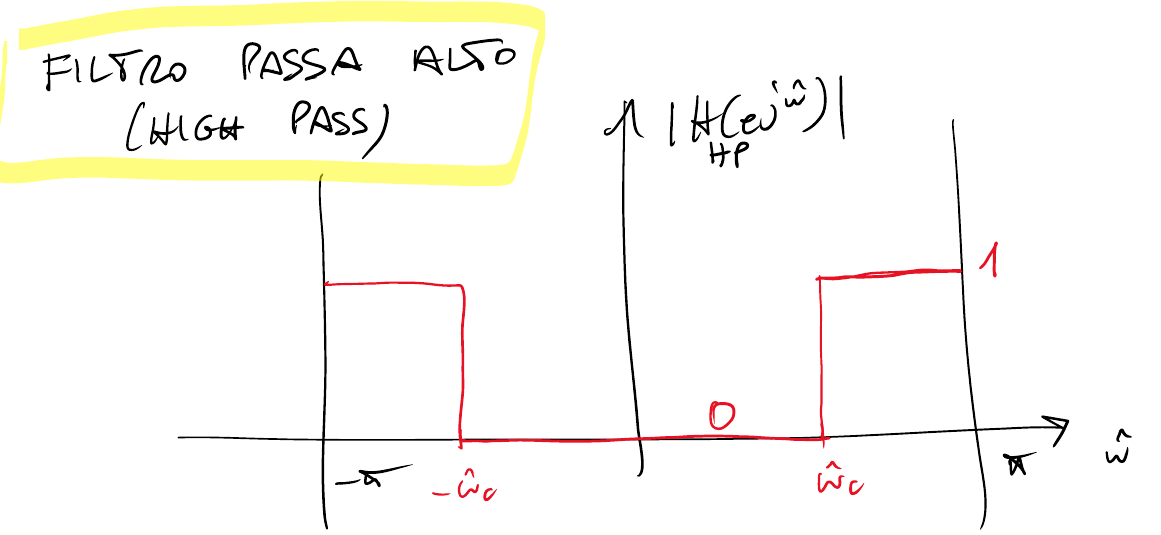
\includegraphics[scale=0.35]{immagini/lez15/passaAlto.jpg}
\end{figure}

Notiamo che se la frequenza di taglio del filtro passa alto e del passa basso e' uguale, allora dato un filtro posso riscrivere l'altro:

\[\begin{split}
    |H_{LP}(e^{j \hat{\omega}})| &= 1 - |H_{HP}(e^{j \hat{\omega}})| \\
    |H_{HP}(e^{j \hat{\omega}})| &= 1 - |H_{LP}(e^{j \hat{\omega}})| 
\end{split}\]

Dove $H_LP$ e' la risposta in frequenza del filtro passa basso e $H_HP$ e' la risposta in frequenza del filtro passa alto.

\subsection{Filtro passa banda (Band Pass)}
A volte serve uccidere frequenze alte e basse ma lasciare una certa banda.

\begin{figure}[ht!]
    \centering
    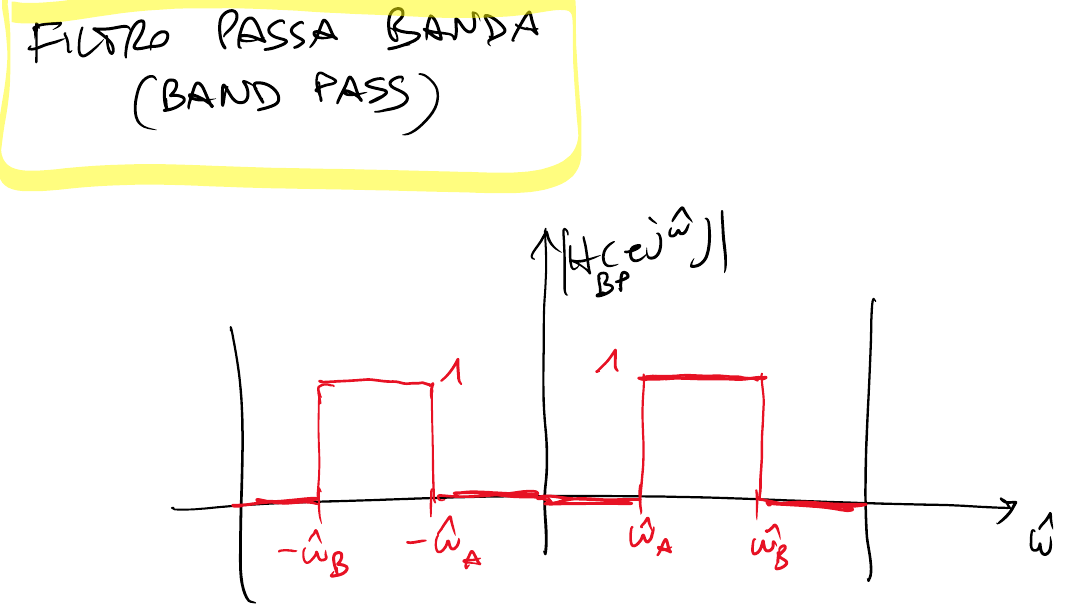
\includegraphics[scale=0.35]{immagini/lez15/passaBanda.jpg}
\end{figure}

\subsection{Filtro blocca banda (Band Block)}
E' il duale del filtro passa banda. Cancella le frequenze che appartengono ad una certa banda. Ad esempio e' usato quando vogliamo cancellare l'interferenza della rete elettrica, (50Hz), nel segnale campionato cancelleremo quel piccolo range di frequenze.

Si chiama Notch Filter quando la banda bloccata e' poco ampia.

\begin{figure}[ht!]
    \centering
    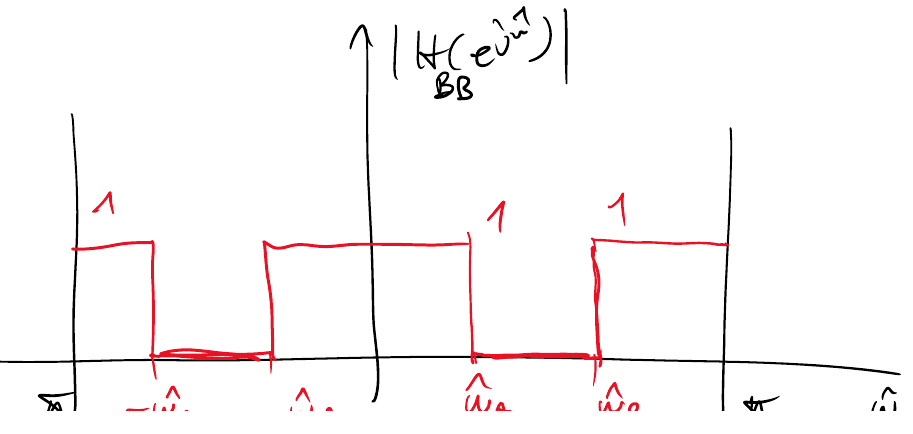
\includegraphics[scale=0.35]{immagini/lez15/bloccaBanda.jpg}
\end{figure}

Anche in questo caso, se la banda e' uguale, posso dato un filtro passa banda posso ottenere il blocca banda e viceversa:

\[
    |H_{BP}(e^{i \hat{\omega}})| = 1 - |H_{BB}(e^{i \hat{\omega}})|
\]



Queste sono definizioni di riferimento, ora vediamo degli esercizi in cui partendo da un equazione alle differenze scriviamo la risposta in frequenza e ne disegniamo il modulo e fase. Infine vedremo a quale filtro ideale assomiglia.

\subsection{Esercizio 1}

Abbiamo un filtro: $y[n] = x[n] + 2x[n-1] + x[n-2]$, quindi quando entra un input in questo sistema ne consideriamo 3 campioni, un presente e due passati, di conseguenza e' un sistema CAUSALE (in quanto dipende solo da presente e passato) e FIR in quanto non e' presente la parte autoregressiva (quella che dipende dall'output). Quindi posso scrivere la risposta all'impulso semplicemente sostituendo $x = \delta$:

\[
    h[n] = 1 \delta[n] + 2 \delta [n-1] + \delta[n-2]
\]

Ora dobbiamo calcolare la risposta in frequenza, per farlo notiamo che dalla sommatoria dobbiamo tenere solo gli elementi in cui la delta e' diversa da 0 (dove vale 1) e sono quelli che annullano la n dentro le varie delta. Mentre come coeficienti moltiplicativi usiamo quelli delle delta:

\[
    H(e^{i \hat{\omega}}) = \sum_{n = +\infty}^{-\infty} x[n] e^{-j \hat{\omega} n} = 1 e^{-j \hat{\omega} 0} + 2 e^{-j \hat{\omega} 1} + 1 e^{-j \hat{\omega} 2}
\]

Ora per trovare il modulo e la fase dobbiamo fare qualche operazione algebrica:

\[
    1 + 2 e^{-j \hat{\omega}} + 1 e^{-j \hat{\omega} 2}
\]

ora il consiglio per risolvere questa equazione e' raccogliere la meta' del termine massimo e vedere cosa succede:

\[
    2e^{-j \hat{\omega}} \{ \frac{e^j \hat{\omega}}{2} + 1 + \frac{e^{-j \hat{\omega}}}{2} \}
\]

Usando Eulero noto che $\frac{e^j \hat{\omega}}{2} + \frac{e^{-j \hat{\omega}}}{2} = \cos(\hat{\omega})$, quindi:

\[
    2e^{-j \hat{\omega}} [1 + \cos(\hat{\omega})]
\]

Ora invece di trasformare in forma polare riscrivo l'equazione in modo che sia scritta in maniera simile alla forma polare, che ricordiamo essere $\phi e^{i \Omega}$, da cui posso ricavare il modulo e la fase:

\[
    (2 + 2 \cos(\hat{\omega}) e^{-j \hat{\omega}}
\]

Dato che $2 + 2 \cos(\hat{\omega} \ge 0$ e' il modulo e la fase sara' $-\hat{\omega}$.

\begin{figure}[ht!]
    \centering
    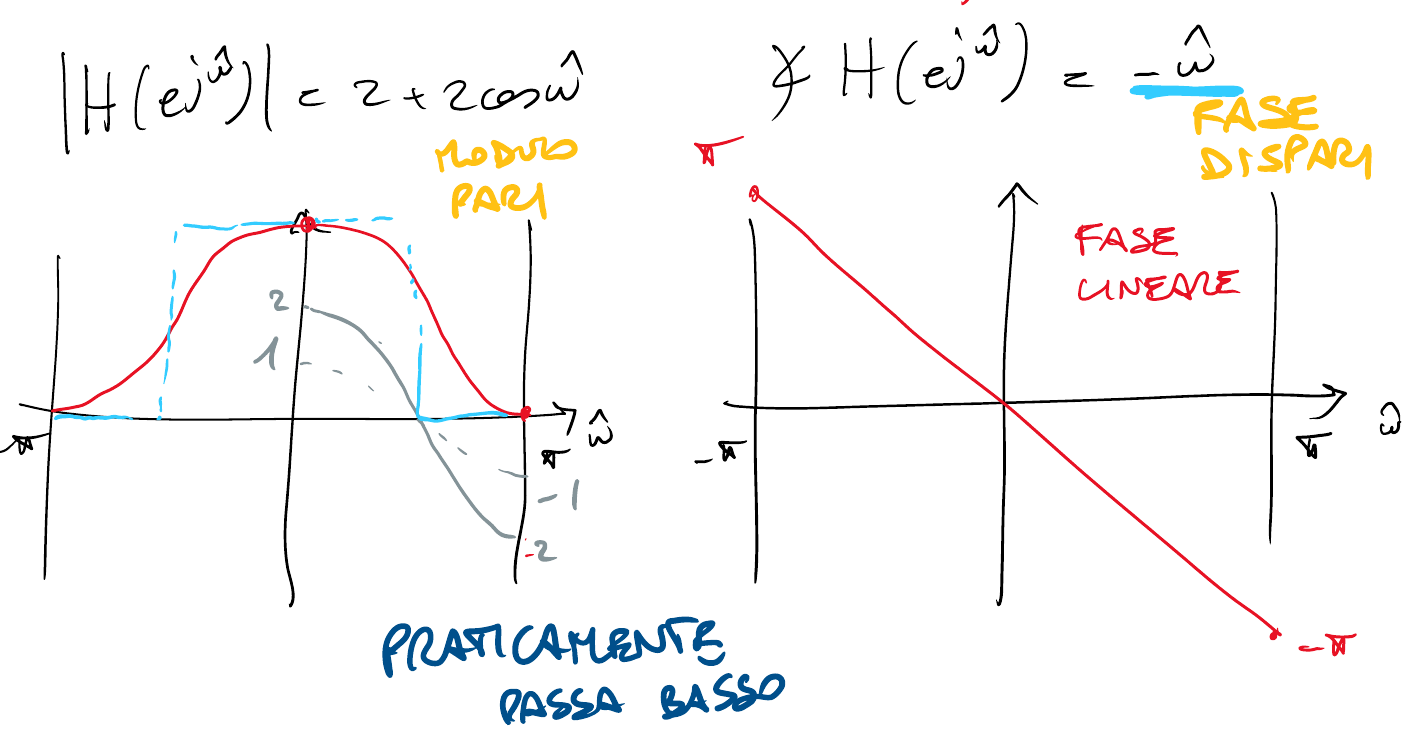
\includegraphics[scale=0.35]{immagini/lez15/es1.jpg}
\end{figure}

Per disegnare i grafici semplicemente dobbiamo disegnare il grafico di ciascuna funzione (modulo e fase), sempre nel periodo della risposta in frequenza $-\pi, +\pi$.
In questo caso notiamo dal grafico del modulo che questo e' un'approssimazione del filtro passa basso.

\subsection{Esercizio 2}
Usiamo lo stesso filtro di prima ma cambiando un segno $y[n] = x[n] - 2x[n-1] + x[n-2]$.
Seguiamo i passaggi fatti in precedenza, quindi inizialmente scriviamo la risposta all'impulso:
\[
    h[n] = 1 \delta[n] - 2 \delta [n-1] + \delta[n-2]
\]

Poi calcoliamo la risposta in frequenza:

\[
    H(e^{i \hat{\omega}}) = \sum_{n = +\infty}^{-\infty} x[n] e^{-j \hat{\omega} n} = 1 e^{-j \hat{\omega} 0} -
    2 e^{-j \hat{\omega} 1} + 1 e^{-j \hat{\omega} 2}
\]

\[\begin{split}
    H(e^{i \hat{\omega}}) &= 1 - 2 e^{-j \hat{\omega}} + 1 e^{-j \hat{\omega} 2} \\
    &= 2e^{-j \hat{\omega}} \{ \frac{e^j \hat{\omega}}{2} - 1 + \frac{e^{-j \hat{\omega}}}{2} \} \\
    &= 2e^{-j \hat{\omega}} [-1 + \cos(\hat{\omega})] \\
\end{split}\]

Ma arrivati a questo punto notiamo che $\cos(\hat{\omega}) - 1$ non puo' essere il modulo, in quanto non e' maggiore di 0. Notiamo che se togliamo un - sarebbe sempre positivo e quindi il modulo:
\[
    -1 e^{-j \hat{\omega}} (2 + 2 \cos(\hat{\omega}))
\]

Ma quel segno meno, come abbiamo sempre fatto, possiamo riscriverlo come $-1 = e^{j\pi}$.

\begin{figure}[ht!]
    \centering
    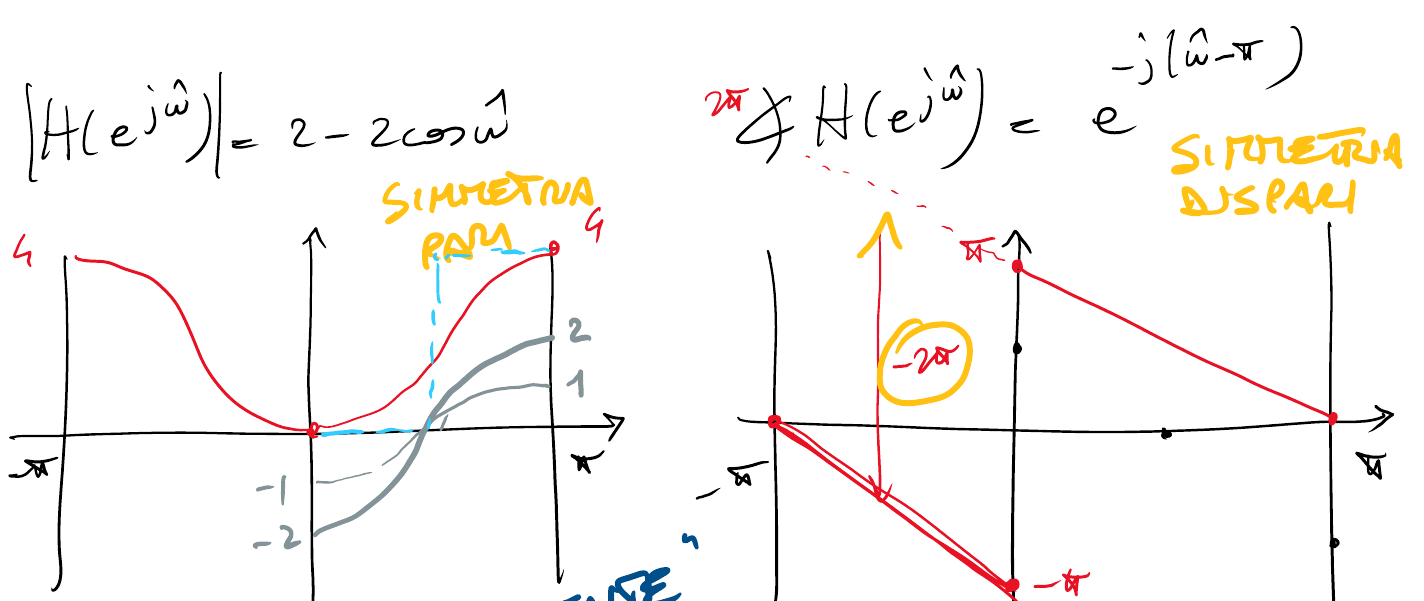
\includegraphics[scale=0.35]{immagini/lez15/es2.jpg}
\end{figure}

Dal grafico del modulo notiamo che e' un'approssimazione del filtro passa alto.

\subsection{Esercizio 3 (Amplificatore Ideale)}
Abbiamo un filtro $y[n] = Ax[n-n_0]$, in cui $n_0$ e' costante ed $A>0$. 
Notiamo subito che se $n_0 \ge 0$ il sistema e' CAUSALE e FIR.
Quello che fa in pratica questo filtro e' prendere il segnale e ritardarlo di n campioni e lo moltiplica di un valore A. Si chiama amplificatore ideale.
Come fatto in precedenza calcoliamo la risposta all'impulso:

\[
    h[n] = A \delta[n-n_0]
\]

Tracciamone il grafico:

\begin{figure}[ht!]
    \centering
    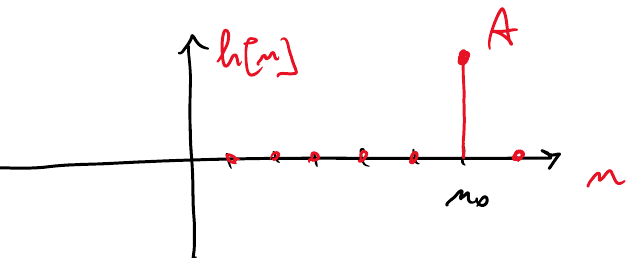
\includegraphics[scale=0.35]{immagini/lez15/es2RispostaImpulso.jpg}
\end{figure}

Troviamo la risposta in frequenza, come prima prendendo dalla sommatoria solo il termine in cui la delta vale 1, in questo caso l'argomento della delta si annulla quando $n = n_0$:

\[
    H(e^{i \hat{\omega}}) = A e^{-j \hat{\omega} n_0}
\]

Da cui ricaviamo il modulo $A$ e la fase $-\hat{\omega}n_0$.





\begin{figure}[ht!]
    \centering
    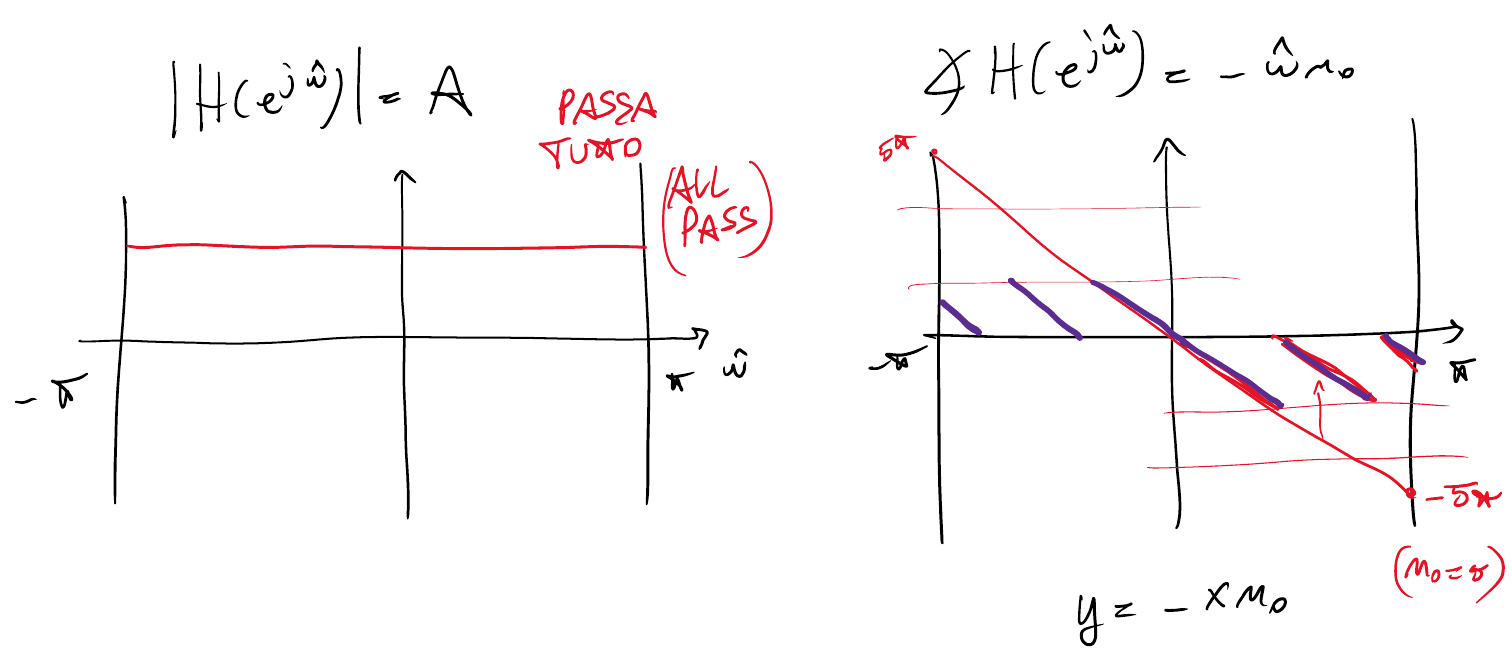
\includegraphics[scale=0.35]{immagini/lez15/es3.jpg}
\end{figure}


\subsection{Esercizio 4}
Partiamo ora dalla risposta all'impulso:

\[
    h[n] =
    \begin{cases}
    \frac{1}{L} \text{ se } 0 \le n \le L-1 \\
    0 \text{ altrimenti } \\
    \end{cases}
\]

Tracciamone il grafico:

\begin{figure}[ht!]
    \centering
    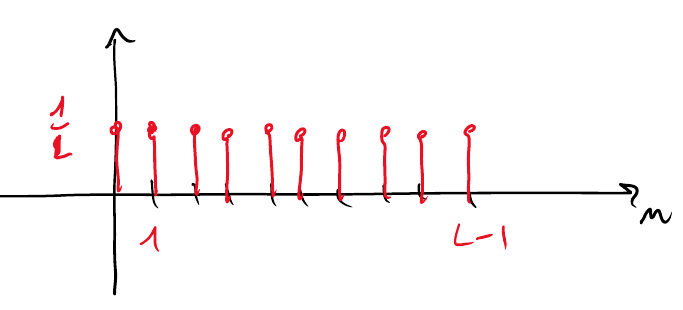
\includegraphics[scale=0.35]{immagini/lez15/es4RispostaImpulso.jpg}
\end{figure}

Il sistema che ha prodotto questa risposta all'impulso sara':

\[
    y[n] = \frac{1}{L} \sum_{k = 0}^{L-1} x[n-k]
\]

Calcolandone la risposta in frequenza:

\[
    H(e^{j \hat{\omega}}) = \sum_{k = 0}^{L-1} \frac{1}{L} e^{-j \hat{\omega} n} = \frac{1}{L} \sum_{k = 0}^{L-1} e^{-j \hat{\omega} n}
\]

Notiamo che questa e' una serie nota $\sum_{k = 0}^{L-1} q^k = \frac{1 - q^L}{1 - q}$, se chiamo $e^{-j \hat{\omega}} = q$, ottengo:

\[
    H(e^{j \hat{\omega}}) = \frac{1}{L} \frac{1 - e^{-j \hat{\omega}L}}{1 - e^{-j \hat{\omega}}}
\]

Ora come prima raccolgo la meta' dell'esponente massimo:

\[\begin{split}
    H(e^{j \hat{\omega}}) =& \frac{1}{L} \frac{e^{-j \hat{\omega} \frac{L}{2}}}{e^{-j \hat{\omega} \frac{L}{2}}} \frac{(e^{j \hat{\omega} \frac{L}{2}} - e^{-j \hat{\omega} \frac{L}{2}})}{(e^{j   \frac{\hat{\omega}}{2}} - e^{-j \frac{\hat{\omega}}{2}})} \frac{\textcolor{red}{2j}}{\textcolor{red}{2j}} \\
    =& e^{-j \hat{\omega} \frac{(L-1)}{2}} \frac{\sin(\hat{\omega} \frac{L}{2})}{\sin(\frac{\hat{\omega}}{2})} \cdot \frac{1}{L}
\end{split}\]

Ottenendo la forma di Dirichlet.

\section{Sistemi in cascata}
Quello che vogliamo fare e' prendere l'output di un sistema e metterlo in input ad un altro sistema LTI.

\begin{figure}[ht!]
    \centering
    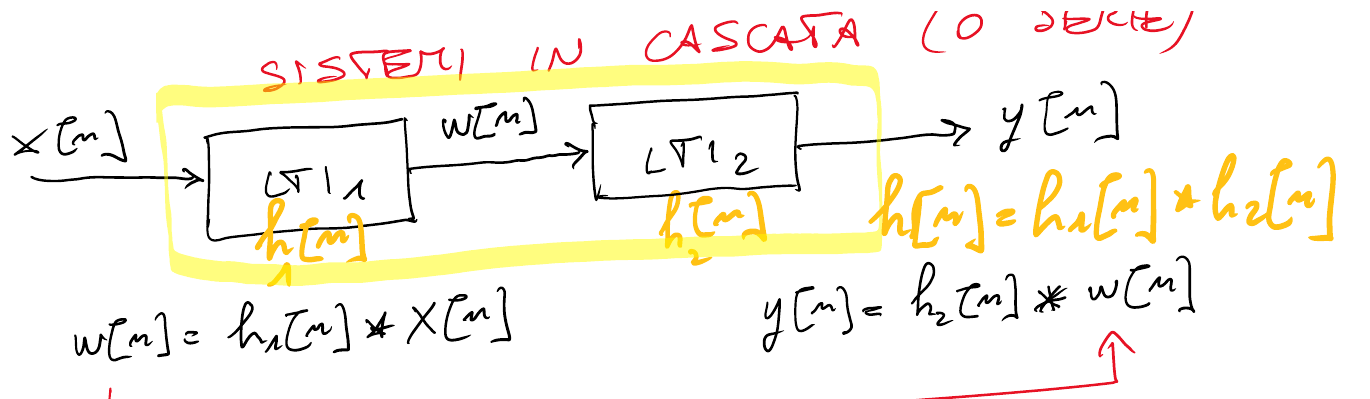
\includegraphics[scale=0.35]{immagini/lez15/sistemiCascata.jpg}
\end{figure}

\[\begin{split}
    y[n] &= h_2[n] * (h_1[n] * x[n]) \\
    y[n] &= (h_1[n] * h_2[n]) * x[n] \\
    h[n] &= h_1[n] * h_2[n]
\end{split}\]

\section{Parallelo di due sistemi}

\begin{figure}[ht!]
    \centering
    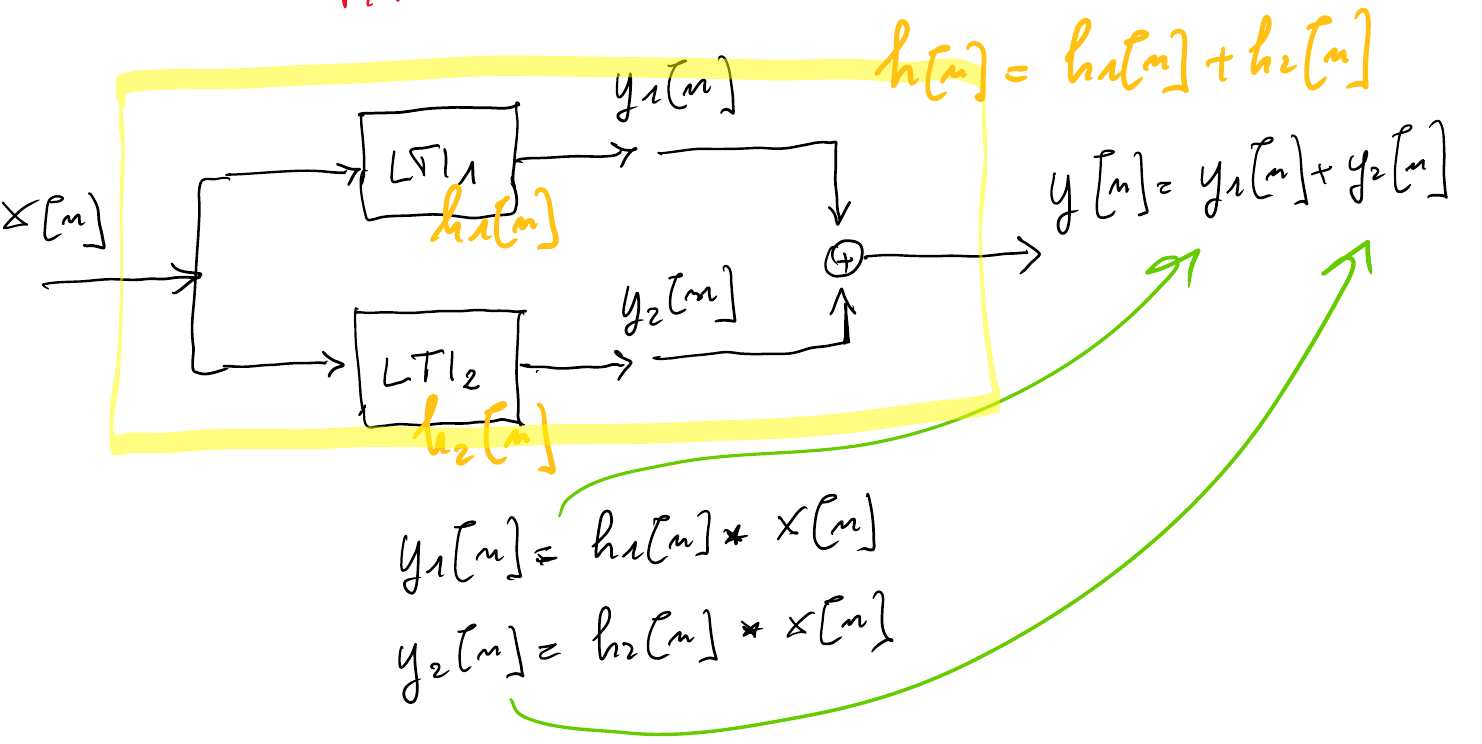
\includegraphics[scale=0.35]{immagini/lez15/paralleloSistemi.jpg}
\end{figure}

\[\begin{split}
    y[n] &= h_1[n] * x[n] + h_2[n] * x[n]\\
    y[n] &= (h_1[n] + h_2[n]) * x[n] \\
    h[n] &= h_1[n] + h_2[n]
\end{split}\]



\chapter{DTFT}
Cominciamo la seconda parte del corso, in questo momento vorremo dato qualunque segnale tempo discreto decomporlo in sinusoidi e vorremo capire quali cosinuosoidi possono fare da filtri per quel segnale e capire meglio cosa fa un sistema.

Inizialmente vediamo a che punto siamo arrivati e capiamo quali segnali abbiamo visto e come possiamo decomporli e ricomporli.

\begin{figure}[ht!]
    \centering
    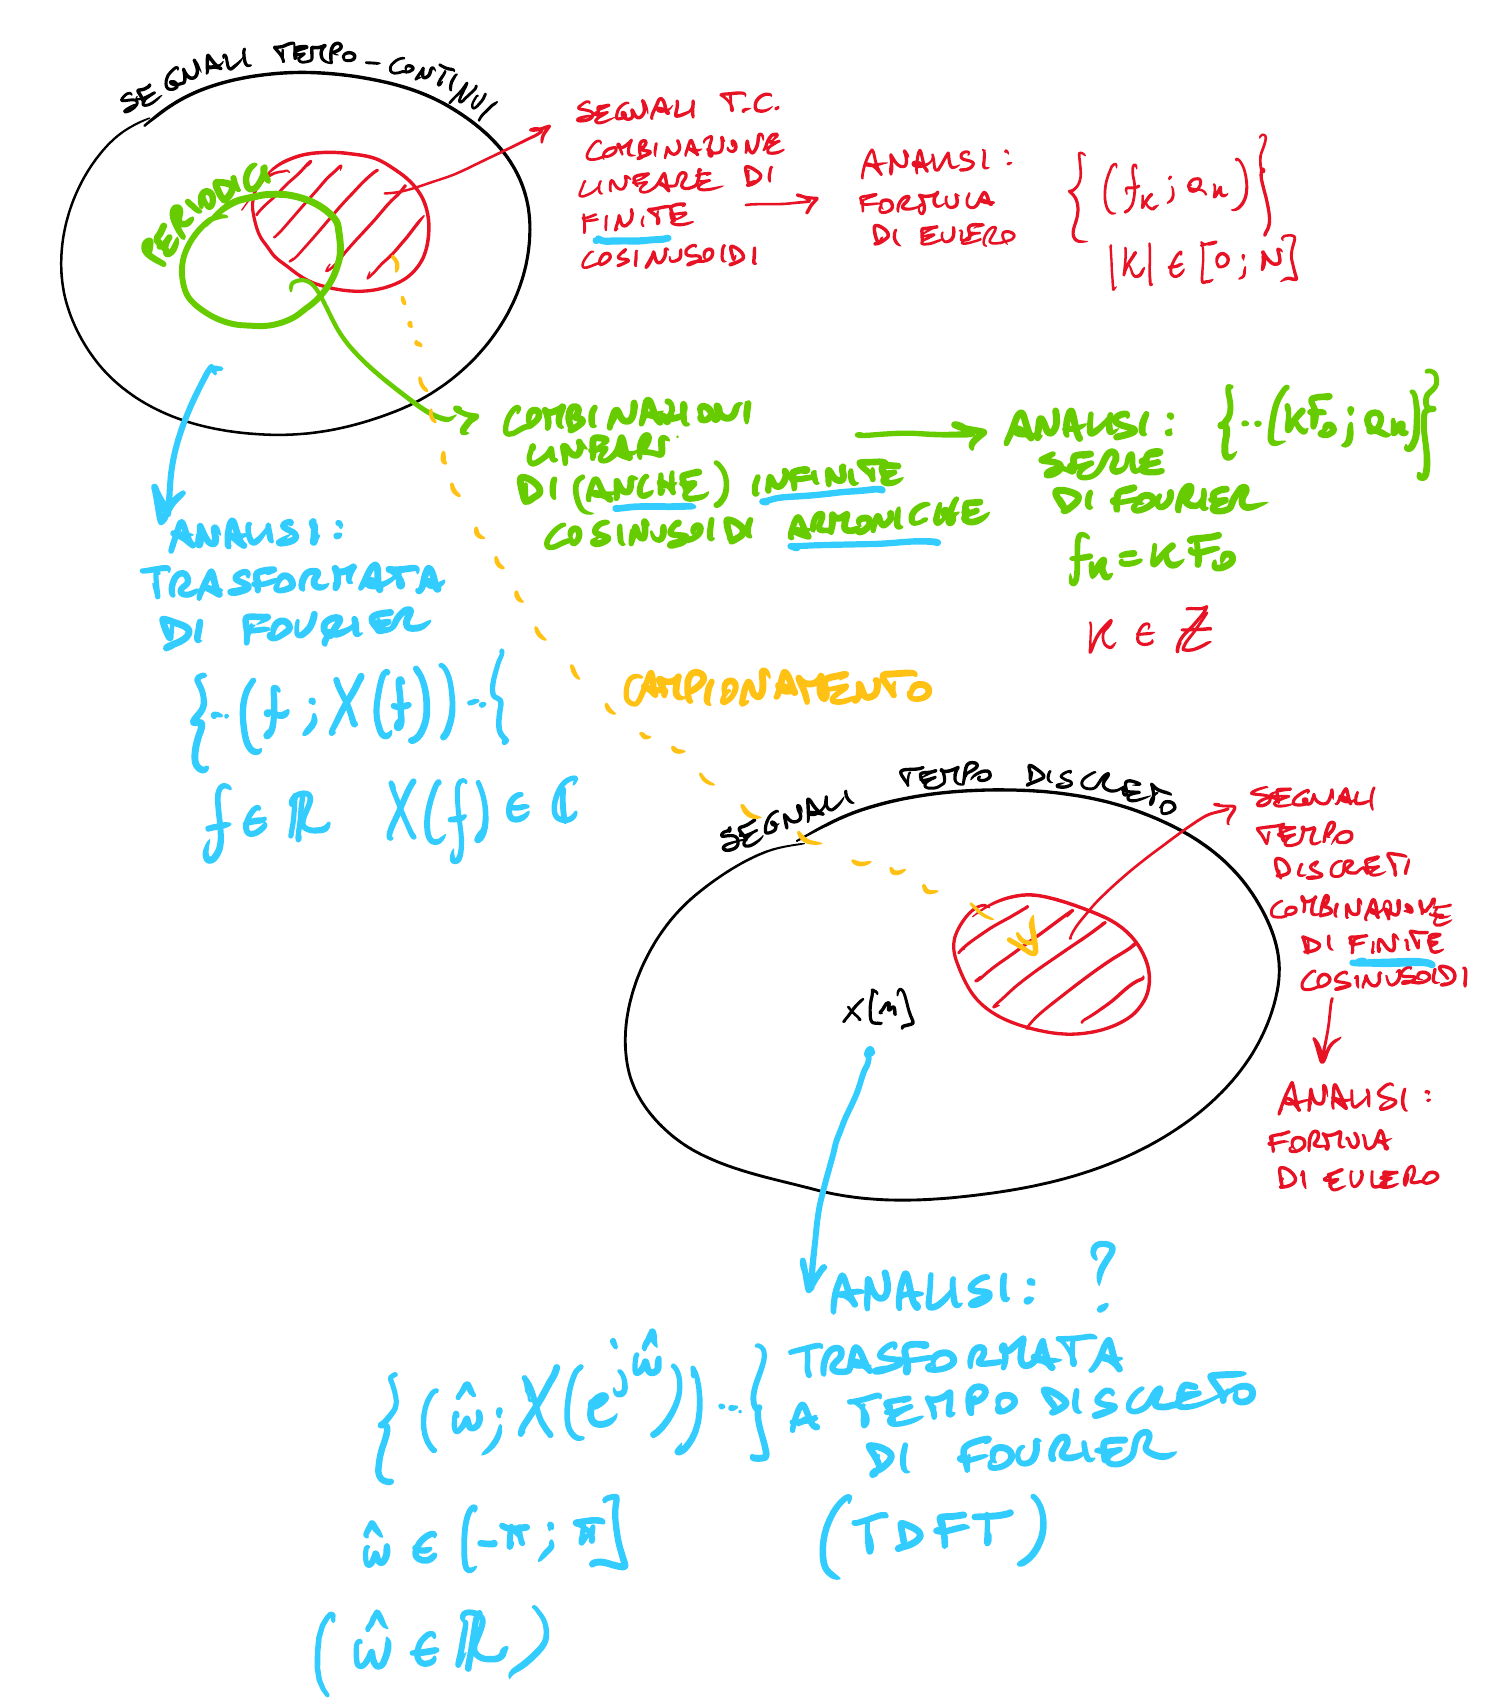
\includegraphics[scale=0.35]{immagini/lez17/segnali.jpg}
\end{figure}

\section{Trasformata a tempo discreto di Fourier (DTFT)}
Studiamo adesso la trasformata a tempo discreto di Fourier, la quale ci permettera' di scrivere lo spettro (fare l'analisi) di un qualunque segnale a tempo discreto.
Analisi:

\begin{equation}
    X(e^{j \hat{\omega}}) = \sum_{n = - \infty}^{+ \infty} x[n] e^{\textcolor{red}{-} j \hat{\omega} n}
\end{equation}

Notiamo inizialmente che questa formula e' molto simile alla risposta in frequenza tranne per un segno -.

Inoltre ricordando la definizione di prodotto scalare tra due segnali tempo discreti:

\[
    <x[n]; y[n]> = \sum_{n = - \infty}^{+ \infty} x[n] \cdot y^*[n]
\]

notiamo che i fasori discreti sono uguali al prodotto scalare tra $x[n]$ e $y^*[n] = e^{j \hat{\omega} n} $, in pratica possiamo riscrivere la DTFT come il prodotto scalare tra un segnale tempo discreto ed una base ortonormale: 
\[
    X(e^{j \hat{\omega}}) = <x[n]; e^{j \hat{\omega} n}>
\]

Inoltre ricordando la serie di Fourier per il tempo continuo, notiamo che c'e' un parallelismo, perche' anche in quel caso l'analisi di un segnale (fatta con un integrale) era uguale al prodotto scalare tra il segnale stesso ed una base ortonormale:

\[
    ak = \frac{1}{T_0} \int_0^{T_0} x(t) \cdot e^{-j 2\pi F_0 k t} dt = <x(t); e^{j 2\pi F_0 k t}>
\]

Formula di SINTESI:

\begin{equation}
    x[n] = \frac{1}{2\pi} \int_{-\pi}^{\pi} X(e^{j \hat{\omega}}) e^{j \hat{\omega} n } \phi \hat{\omega}
\end{equation}

Anche per quanto riguarda la forumla di sintesi notiamo il parallelismo con la sintesi della serie di Fourier per i segnali a tempo continuo:

\[
    x(t) = \sum_{k = - \infty}^{+ \infty} ak e ^{j 2\pi F_0 k t}
\]

Vediamo anche se consideriemo le frequenze come cambia la formula di Sintesi della DTFT:

\[\begin{split}
    \hat{\omega} &= 2\pi \hat{f} \\
    d \hat{\omega} &= 2\pi d \hat{f} \\
    &= 1 \int_{-\frac{1}{2}}^{\frac{1}{2}} X(e^{j 2\pi \hat{f}}) e^{j 2\pi \hat{f}} d \hat{f}
\end{split}\]

Elenchiamo adesso le proprieta' della DTFT.

\subsection{DTFT e' periodica di periodo $2\pi$}

Per verificare che sia vero proviamo a calcolare la DTFT in multipli di $2\pi$ per vedere se otteniamo lo stesso risultato, dove $h \in \mathbf{Z}$:

\[
    X(e^{j (\hat{\omega} + 2\pi h)}) = \sum_{n = - \infty}^{+ \infty} x[n] e^{-j n (\hat{\omega} + 2\pi h)} = \sum_{n = - \infty}^{+ \infty} x[n] e^{-j \hat{\omega} n} \cdot e^{-j n 2\pi h}
\]

A questo punto notiamo che il termine $e^{-j n 2\pi h}$ e' il numero 1, quindi abbiamo ottenuto esattamente la DTFT.

\subsection{La DTFT gode della proprieta' si simmetria coniugata se $x[n]$ e' reale}

Quello che significa questa proprieta' e':

\[
     X(e^{j \hat{\omega}}) =  X^*(e^{-j \hat{\omega}})
\]

Il corollario di questa proprieta' e' che la parte reale di $ X(e^{j \hat{\omega}})$, ovvero il modulo, e' una funzione pari, mentre la parte immaginaria di $ X(e^{j \hat{\omega}})$, la fase, e' una funzione dispari.

\subsection{La DTFT e' un operatore lineare}
Dati due coeficienti $\alpha, \beta \in \mathbf{R}$ se sappiamo che:

\[\begin{split}
    x_1[n] &\xrightarrow[]{\text{DTFT}} X_1(e^{j \hat{\omega}}) \\
    x_2[n] &\xrightarrow[]{\text{DTFT}} X_2(e^{j \hat{\omega}}) 
\end{split}\]

allora

\[
    \alpha x_1[n] + \beta x_2[n] x_1[n] \xrightarrow[]{\text{DTFT}} \alpha X_1(e^{j \hat{\omega}}) + \beta X_2(e^{j \hat{\omega}})
\]

\subsection{Se esiste la DTFT di $x[n]$, allora e' unica}
Dimostriamola per assurdo, dati due segnali li trasformiamo in una DTFT comune:

\[\begin{split}
    x_1[n] &\xrightarrow[]{\text{DTFT}} X(e^{j \hat{\omega}}) \\
    x_2[n] &\xrightarrow[]{\text{DTFT}} X(e^{j \hat{\omega}}) 
\end{split}\]

Ma se consideriamo un segnale che e' la differenza tra i due precedenti otteniamo ovviamente 0, in quanto, utilizzando la proprieta' di linearita' appena descritta la DTFT dei due e' uguale:

\[
    x[n] = x_1[n] - x_2[n] \xrightarrow[]{\text{DTFT}} X(e^{j \hat{\omega}})- X(e^{j \hat{\omega}}) = 0
\]

Ma questo vorrebbe dire che esiste un segnale la cui DTFT e' 0, ma questo puo' succedere solo se i due segnali sono uguali.

\subsection{Esempio 1}
Guardiamo ora lo spettro di alcuni segnali cosinusoidali.
Inizialmente consideriamo una delta traslata di $n_0$:

\begin{figure}[ht!]
    \centering
    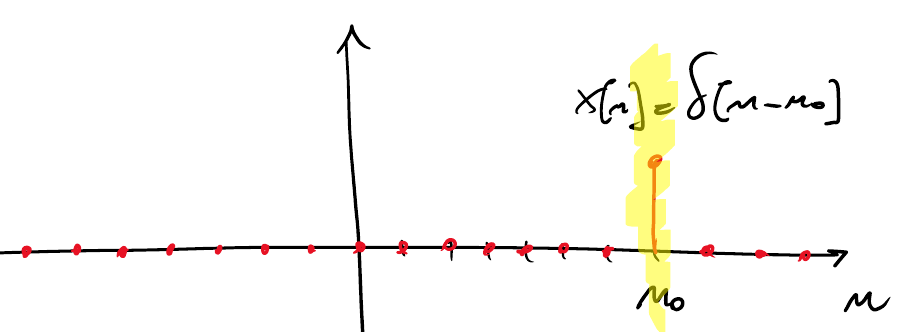
\includegraphics[scale=0.35]{immagini/lez17/esempio1.jpg}
\end{figure}

Per calcolare lo spettro applichiamo troviamo la DTFT del segnale applicando la definizione:

\[
    X(e^{j \hat{\omega}}) = \sum_{-\infty}^{+ \infty} \delta[n - n_0] e^{-j \hat{\omega} n}
\]

Ma sappiamo che la delta vale sempre zero tranne in $n_0$, di conseguenza la sommatoria si risolve in:

\[
    X(e^{j \hat{\omega}}) = e^{-j \hat{\omega} n_0}
\]

Tracciamo il grafico del modulo e della fase, il modulo e' costante ed e' 1 (ricordiamo che il modulo e' il numero intero che moltiplica l'esponenziale), mentre la fase e' uguale alla retta $y = -n_0 x$:

\begin{figure}[ht!]
    \centering
    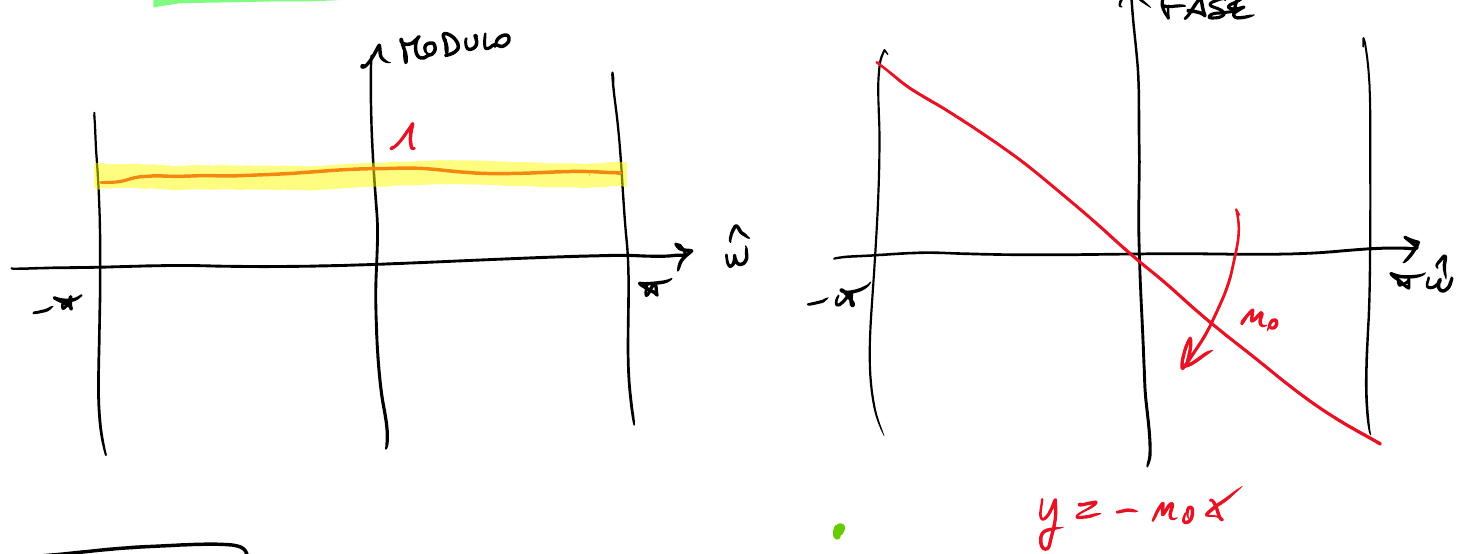
\includegraphics[scale=0.35]{immagini/lez17/moduloFaseEs1.jpg}
\end{figure}

\subsection{Esempio 2}
Come secondo esempio consideriamo il segnale esponenziale moltiplicato per il segnale calino:

\[
    x[n] = a^n \cdot u[n]
\]



\begin{figure}[ht!]
    \centering
    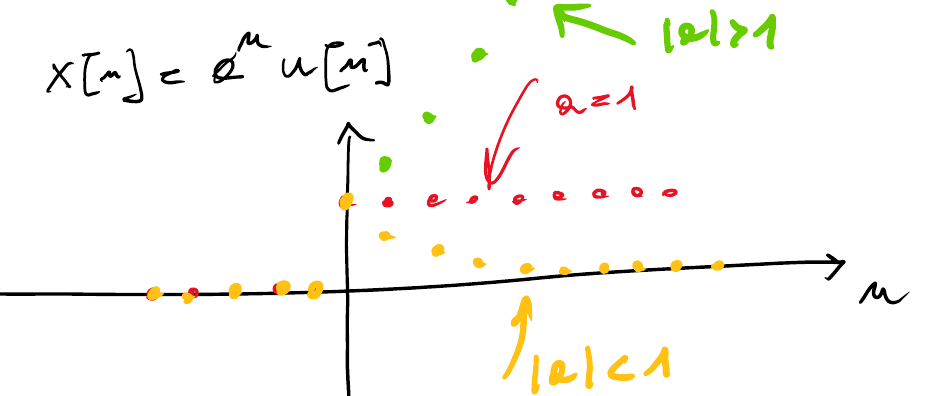
\includegraphics[scale=0.35]{immagini/lez17/esempio2.jpg}
\end{figure}

Come prima calcoliamo la DTFT del segnale applicando la formula:

\[
    DTFT\{ x[n] = a^n \cdot u[n] \} = \sum_{n = -\infty}^{+ \infty} a^n \cdot u[n] e^{-j \hat{\omega} n}
\]

Modifichiamo gli estremi della sommatoria dato che se $n<0$ la funzione non esiste, inoltre utilizziamo la sommatoria nota $\sum_{k=0}^{L-1}q^L = \frac{1-q^L}{1-q}$:

\[
    \sum_{n = 0}^{+\infty}(a e^{-j \hat{\omega}})^n = \lim_{N\to\infty}\frac{1 -(a e^{-j \hat{\omega}})^n}{a e^{-j \hat{\omega}}}
\]

Se $|a e^{-j \hat{\omega}}| < 1$ allora otteniamo $\frac{1}{1 - ae^{-j\hat{\omega}}}$

\section{Esempi con luce}
Vediamo un parallelismo tra l'analisi tramite DTFT di un segnale con la scomposizione di un fascio di luce bianca tramite un primsa e vediamo che decomponendo un segnale tramite la DTFT otteniamo lo spettro.

\begin{figure}[ht!]
    \centering
    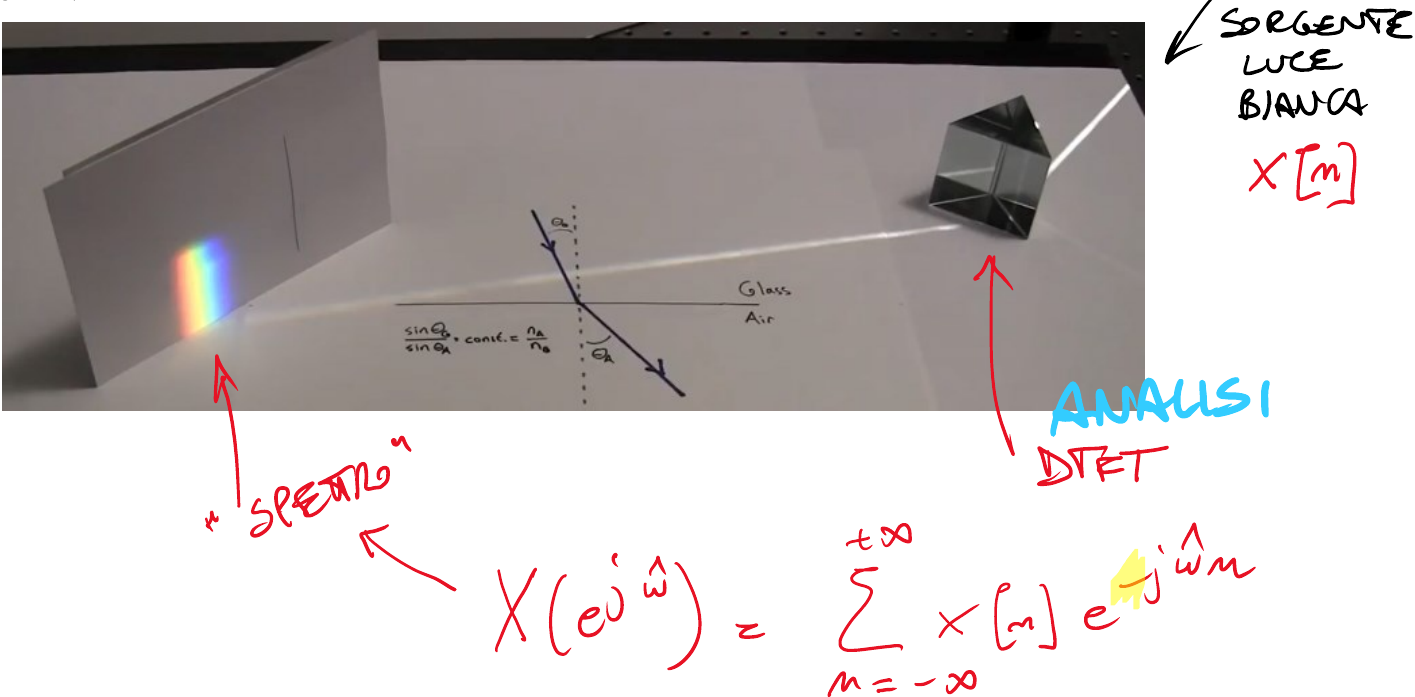
\includegraphics[scale=0.35]{immagini/lez18/sintesi.jpg}
\end{figure}

Quando invece vogliamo ricomporre lo spettro di un segnale utilizziamo la trasformata inversa IDTFT:

\begin{figure}[ht!]
    \centering
    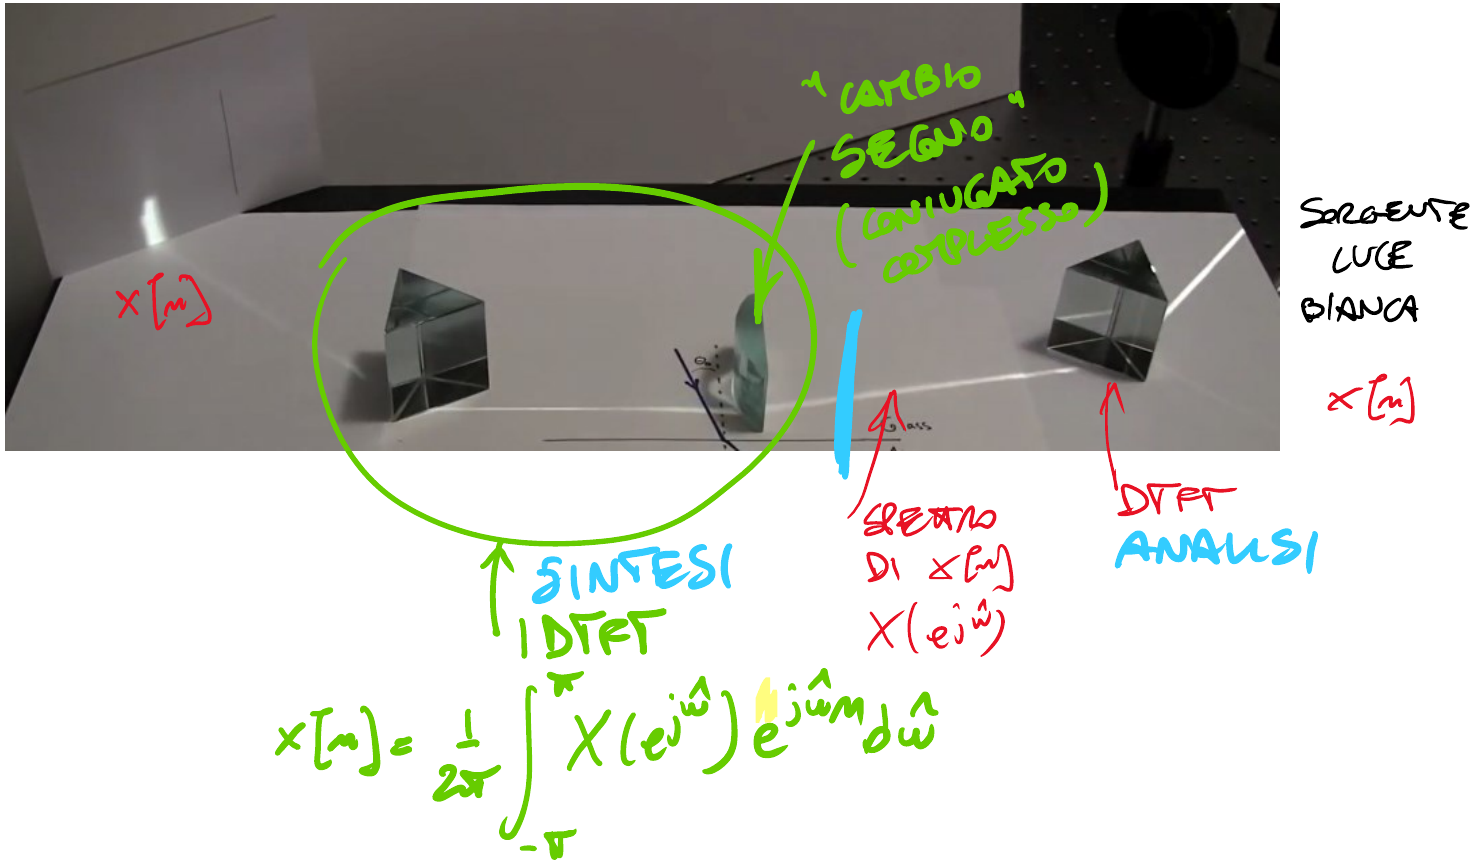
\includegraphics[scale=0.35]{immagini/lez18/analisiSintesi.jpg}
\end{figure}

La formula della IDTFT:

\begin{equation}
    x[n] = \frac{1}{2\pi} \int_{-\pi}^{\pi} X(e^{j \hat{\omega}}) e^{j \hat{\omega}n} d \hat{\omega}
\end{equation}

\section{Esempio}
Partiamo dal grafico del modulo e della fase di un segnale, e notiamo subito che assomiglia ad un filtro passa basso, di conseguenza le frequenze comprese tra $-\hat{w}_c$ e $\hat{w}_c$ passano, le altre vengono eliminate

\begin{figure}[ht!]
    \centering
    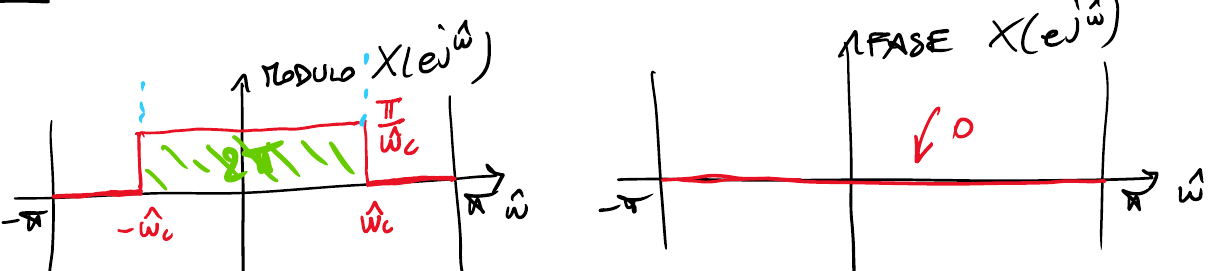
\includegraphics[scale=0.35]{immagini/lez18/esempio3ModuloFase.jpg}
\end{figure}

Utilizziamo la formula della IDTFT per ricostruire il segnale:

\[\begin{split}
    x[n] &= \frac{1}{2\pi} \int_{-\pi}^{\pi} \mbox{BOX}_{\hat{w}_c}(t) e^{j \hat{\omega}n} d \hat{\omega} = \frac{1}{2\pi} \int_{-\hat{w}_c}^{w_c} \frac{\pi}{\hat{w}_c} e^{j \hat{\omega}n} d \hat{\omega} \\
    &= \frac{1}{2 \hat{\omega}_c} [\frac{e^{j \hat{\omega} n}}{jn}]_{-\hat{\omega}}^{\hat{\omega}_c} = \frac{1}{2\hat{\omega}} \{ \frac{e^{j \hat{\omega}_c n}}{jn} - \frac{e^{-j \hat{\omega}_c n}}{jn} \} \\
    &= \frac{\sin \hat{\omega}_c n}{\hat{\omega}_ c} = sinc(\hat{\omega}_c n)
\end{split}\]

\begin{figure}[ht!]
    \centering
    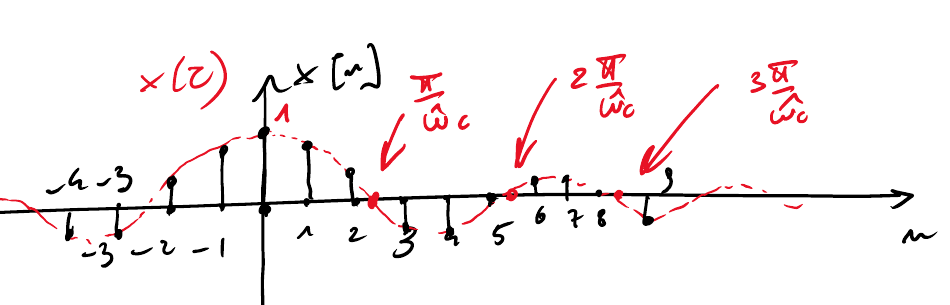
\includegraphics[scale=0.35]{immagini/lez18/casoGenerale.jpg}
\end{figure}

Quindi la ricostruzione di un filtro passa basso e' un sinc.

\medskip
\medskip
\medskip
\medskip
\medskip
\medskip
\medskip
\medskip
\medskip
\medskip
\medskip
\medskip
\medskip
\medskip
\medskip
\medskip
\medskip
\medskip
\medskip
\medskip
\medskip
\medskip
\medskip
\medskip
\medskip
\medskip
\medskip
\medskip
\medskip
\medskip
\medskip

Ora consideriamo dei casi particolari di questo filtro, inizialmente vediamo quando facciamo tendere $-\hat{w}_c$ e $\hat{w}_c$ a 0:

\begin{figure}[ht!]
    \centering
    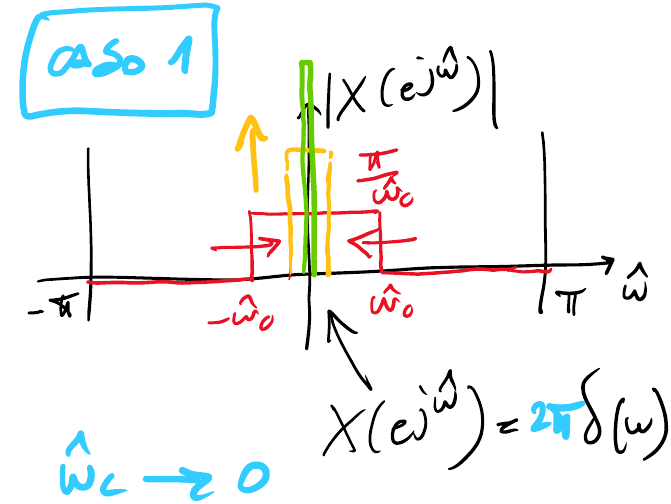
\includegraphics[scale=0.35]{immagini/lez18/casoParticolare1.jpg}
\end{figure}

Quello che succede e' che stringo il BOX e piu' lo stringo piu' l'altezza deve aumentare, ma l'area rimane uguale:

\begin{figure}[ht!]
    \centering
    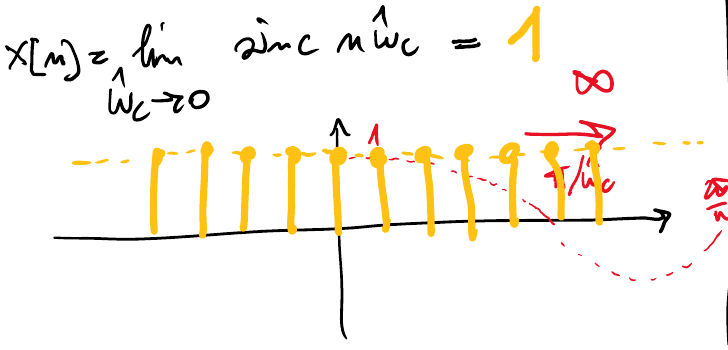
\includegraphics[scale=0.35]{immagini/lez18/estremoCaso1.jpg}
\end{figure}

Come secondo caso particolare invece vediamo cosa succede quando facciamo tendere $-\hat{w}_c$ e $\hat{w}_c$ a $\pi$, quello che succede e' che diminuisce l'altezza del BOX e diminuisce l'altezza.

\begin{figure}[ht!]
    \centering
    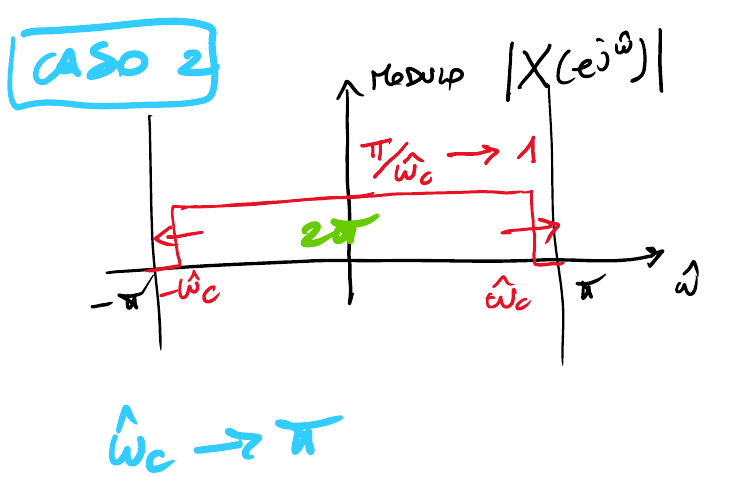
\includegraphics[scale=0.35]{immagini/lez18/casoParticolare2.jpg}
\end{figure}

Quello che otteniamo e' un sinc in cui sostituiamo $\hat{\omega}_c = \pi$, quindi e' una delta centrata in 0:

\begin{figure}[ht!]
    \centering
    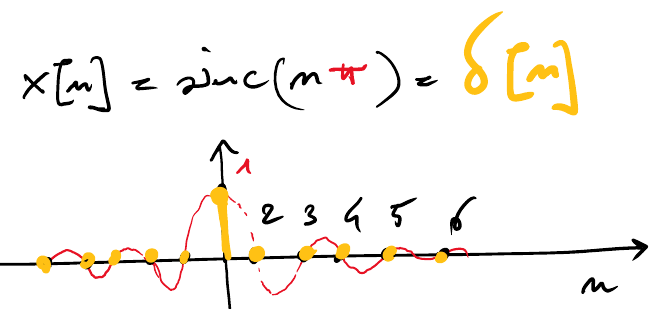
\includegraphics[scale=0.35]{immagini/lez18/estremoCaso2.jpg}
\end{figure}

\section{Delta di Dirac (funzione continua)}

E' una funzione generalizzata (o distribuzione), e' un'estensione al limite di una funzione che possiamo usare solo in composizione lineare.

\begin{figure}[ht!]
    \centering
    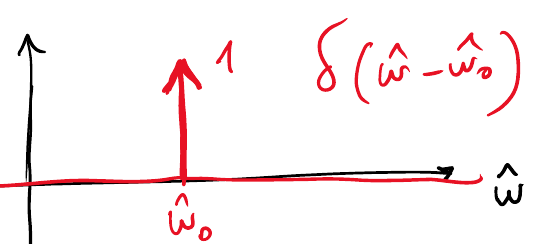
\includegraphics[scale=0.35]{immagini/lez18/deltaDirac.jpg}
\end{figure}

\subsection{Dimostrazione Empirica}
La definizione empirica di delta di Dirac e' che abbiamo una quantita' ce vale 0 tranne tra $-\hat{w}_c$ e $\hat{w}_c$ a $\pi$ dove vale $\frac{\pi}{\hat{\omega}_c}$, se consideriamo il limite di $\hat{\omega}_c \rightarrow 0$ il rettangolo si stringe alla forma limite in cui tende ad essere una $\delta(\hat{\omega})$.

\begin{figure}[ht!]
    \centering
    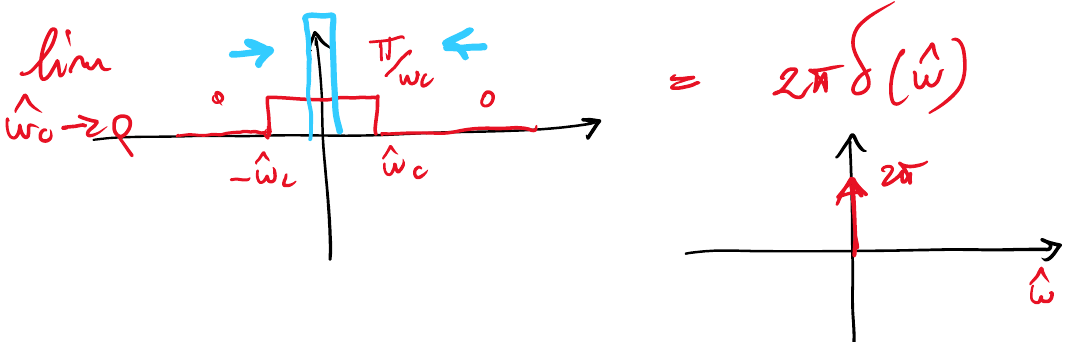
\includegraphics[scale=0.35]{immagini/lez18/diracEmpirica.jpg}
\end{figure}

\subsection{Definizione che ragiona sull'area finita}
La proprieta' del setaccio:

\[
    \int_{-\pi}^{\pi} f(\hat{\omega}) \delta(\hat{\omega} - \hat{\omega}_0) d \hat{\omega} = f(\hat{\omega})
\]

Quello che dimostra e' che la delta di Dirac e' l'integrale definito nel dominio della funzione.

\subsubsection{2}
\[
    \int_{-\pi}^{\pi} \delta(\hat{\omega} - \hat{\omega}_0) d \hat{\omega} = 1
\]

\subsubsection{3}
\[\begin{split}
    e^{j \hat{\omega}_0 n} \xleftarrow[\xrightarrow{DTFT}]{IDTFT} 2\pi \delta(\hat{\omega} - \hat{\omega}_0)
\end{split}\]

\section{Condizione sufficiente di esistenza della DTFT ("equivalente" condizioni di Dirichlet)}

Se sappiamo decomporre i segnali in componenti ortogonali capiamo come progettare un filtro. Il filtraggio in frequenza e' simile al filtraggio nel tempo, e' la stessa cosa letta in modi diversi. L'operatore per l'analisi di qualunque segnale a tempo discreto e' la DTFT, mentre l'operatore per la sintesi di qualunque segnale a tempo discreto e' la IDTFT (inverso DTFT).
Dati questi operandi troviamone le proprieta'.
Per ora non ci siamo dati condizioni di esistenza, quando possiamo applicare questi operatori?

La condizione sufficiente per l'esistenza della DTFT e' l'assoluta sommabilita' del segnale (notiamo che la condizione di Dirichlet era l'integrale nel periodo):

\begin{equation}
    \sum_{-\infty}^{+\infty} |x[n]| < + \infty
\end{equation}

Ci garantisce che qualunque segnale reale che ha un inizio ed una fine e' assolutamente sommabile e di conseguenza decomponibile. Questa condizione e' lasca nella realta', infatti nelle applicazioni pratiche si da per scontato che esista la DTFT.

Cerchiamo di darne circa una dimostrazione, vogliamo garantire che esiste (una serie esiste quando converge ad un valore finito) una DTFT, ovvero che $\sum_{-\infty}^{+\infty} x[n] e^{-j \hat{\omega}_n} = \mbox{DTFT}\{ x[n] \}$.
Quindi vuol dire che per ogni valore di $\hat{\omega}_n$ la sommatoria converge, quindi il modulo converge ma la fase puo' ruotare all'infinito, ma essendo periodica sara' sempre un multiplo di $2\pi$. Esiste significa che $|\sum_{-\infty}^{+\infty} x[n] e^{-j \hat{\omega}_n}| < +\infty$.

Se esiste la sommatoria applichiamo delle proprieta' sui coeficenti:

\[\begin{split}
    &|\sum_{-\infty}^{+\infty} x[n] e^{-j \hat{\omega}_n}| \le \sum_{-\infty}^{+\infty} |x[n] e^{-j \hat{\omega}_n}| = \sum_{-\infty}^{+\infty} |x[n]| \cancel{|e^{-j \hat{\omega}_n}|} \\
    &|\sum_{-\infty}^{+\infty} x[n] e^{-j \hat{\omega}_n}| \le \sum_{-\infty}^{+\infty} |x[n]| < + \infty
\end{split}\]

\subsection{Ulteriori riflessioni su cosa voglia dire analizzare e sintetizzare un segnale $x[n]$}

Nella prima parte del corso abbiamo parlato della sintesi tramite la serie di Fourier:

\[
    x(t) = \sum_{k = -\infty}^{+\infty} a_k e^{j 2\pi F_0 k t}
\]

mentre ora per i segnali a tempo discreto usiamo la DTFT:

\[
    x[n] = \frac{1}{2\pi} \int_{-\pi}^{+\pi} X(e^{j \hat{\omega}}) e^{j \hat{\omega}n} d\hat{\omega}
\]

In tutti e due i casi abbiamo una base su cui ricostruire il segnale, prendiamo la proiezione scalare del segnale sulla base per la base stessa.

\section{Proprieta' del ritardo temporale}
Dato un segnale e la sue DTFT lo chiameremo coppia di Fourier, se applichiamo un ritardo $n_0$ al segnale originale, otterremo :

\[\begin{split}
   x[n] &\leftrightarrow X(e^{j \hat{\omega}}) \\
   x[n - n_0] &\leftrightarrow X(e^{j \hat{\omega}}) \cdot e^{-j \hat{\omega} n_0}
\end{split}\]

Quello che succede e' che moltiplichiamo la DTFT per un termine di fase lineare che dipende da $n_0$.
Dimostriamolo:

\[\begin{split}
    DTFT\{x[n-n_0]\} &= \sum_{n = -\infty}^{+\infty} x[n-n_0] e^{-j \hat{\omega} n_0} \\
    &\mbox{Chiamiamo  } m = n - n_0 \\
    &= \sum_{m = -\infty}^{+\infty} x[m] e^{-j \hat{\omega} (m + n_0)} \\
    &= \{ \sum_{m = -\infty}^{+\infty} x[m] e^{-j \hat{\omega} m} e^{-j \hat{\omega}n_0} \}
\end{split}\]

\begin{figure}[ht!]
    \centering
    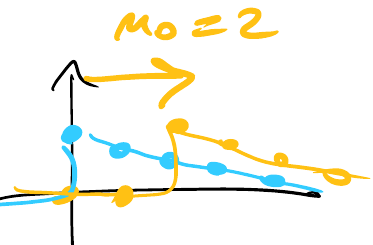
\includegraphics[scale=0.2]{immagini/lez20/ritardoTemporale.jpg}
\end{figure}


\section{Proprieta' del ritardo in frequenza}

\[\begin{split}
   x[n] &\leftrightarrow X(e^{j \hat{\omega}}) \\
   x[n] e^{j \hat{\omega}_0 n} &\leftrightarrow X(e^{j (\hat{\omega} - \hat{\omega}_0}))
\end{split}\]

\begin{figure}[ht!]
    \centering
    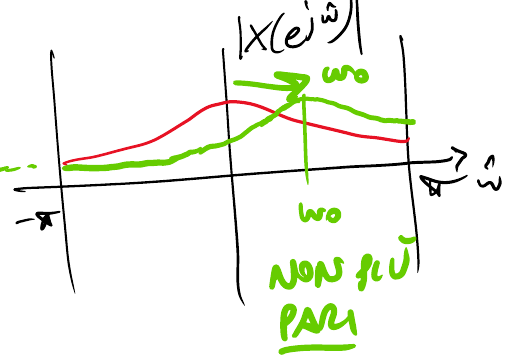
\includegraphics[scale=0.35]{immagini/lez20/ritardoFrequenza.jpg}
\end{figure}

Dimostriamolo:

\[\begin{split}
    IDTFT\{ X(e^{j(\hat{\omega}-\hat{\omega}_0)}) \} &= \frac{1}{2\pi} \int_{-\pi}^{\pi} X[e^{j(\hat{\omega}-\hat{\omega}_0)}] e^{j \hat{\omega}n} d\hat{\omega} \\
    &\mbox{Chiamiamo  } \hat{\Omega} = \hat{omega} - \hat{\omega}_0 \mbox{ e } d\hat{\omega} = d\hat{\Omega} \\
    &= frac{1}{2\pi} \int_{-\pi}^{\pi} X[e^{j(\hat{\Omega}-\hat{\omega}_0)}] e^{j (\hat{\Omega} + \hat{\omega})n} d\hat{\Omega} \\
    &= \{ frac{1}{2\pi} \int_{-\pi}^{\pi} X[e^{j(\hat{\Omega}-\hat{\omega}_0)}] e^{j\hat{\Omega}n} d\hat{\Omega} \} e^{j \hat{\omega}_0 n}
\end{split}\]

\section{Modulazione d'ampiezza}
Possiamo estendere il discorso fatto nel tempo continuo, cosa succede quando prendo il segnale e lo moltiplico per una portante, la modulazione d'ampiezza.
$x[n]$ modula l'ampiezza mentre $\cos (\hat{\omega}_0 n)$ e' la portante, noi vogliamo trovare lo spettro del segnale, e per farlo usiamo la DTFT:

\[\begin{split}
    y[n] &= x[n] \cos(\hat{\omega}_0 n) \\
    &\mbox{scomponiamo il coseno con la formula di Eulero} \\
    &= \frac{1}{2} x[n](e^{j \hat{\omega}_0 n} + e^{-j \hat{\omega}_0 n}) \\
    &= \frac{1}{2} x[n] e^{j \hat{\omega}_0 n} + \frac{1}{2} x[n] e^{-j \hat{\omega}_0 n} \\
    &\mbox{Ora calcoliamo la DTFT del segnale, per farlo usiamo la proprieta' della linearita'} \\
    DTFT\{ y[n] \} &= \frac{1}{2} \mbox{DTFT} \{ x[n] e^{j \hat{\omega}_0 n} \} + \frac{1}{2} \mbox{DTFT} \{x[n] e^{-j \hat{\omega}_0 n}\} \\
    &= \frac{1}{2} X[e^{j(\hat{\omega} - \hat{\omega}_0)}] + \frac{1}{2} X[e^{j(\hat{\omega} + \hat{\omega}_0)}]
\end{split}\]

\begin{figure}[ht!]
    \centering
    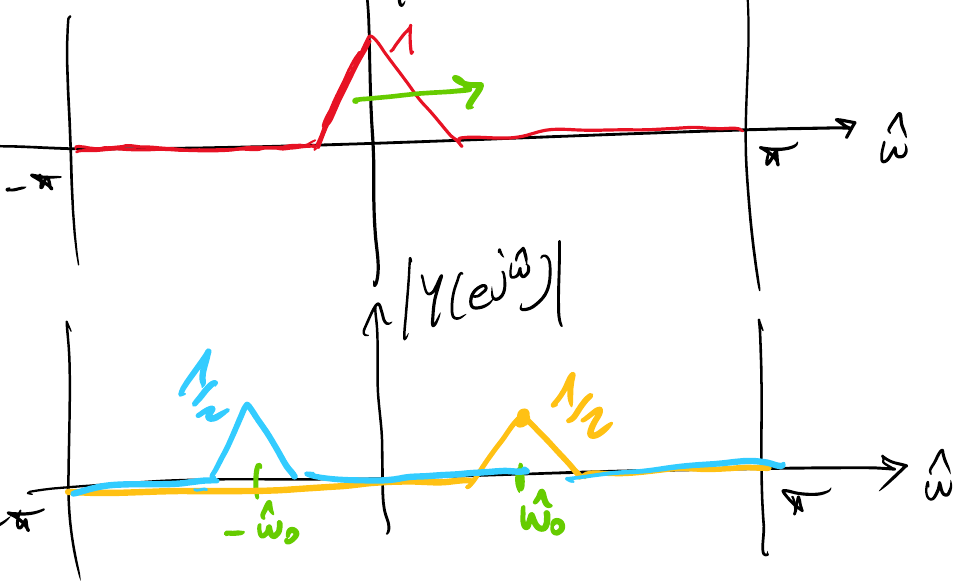
\includegraphics[scale=0.35]{immagini/lez20/modulazioneAmpiezza.jpg}
\end{figure}

\section{Spettro di un coseno}
Ricordiamo:

\[\begin{split}
    x[n] &= 1 \leftrightarrow X(e^{j \hat{\omega}}) = \delta(\hat{\omega})2\pi \\
    y[n] &= x[n] \cos(\hat{\omega}_0 n) = \cos(\hat{\omega}_0 n)
\end{split}\]

Ora vogliamo calcolare la DTFT del coseno, ed intuitivamente abbiamo l'idea che il risultato di una decomposizione di un coseno deve essere un coseno, verifichiamolo:

\[\begin{split}
    \mbox{DTFT}\{ \cos(\hat{\omega}_0 n) \} &= \mbox{DTFT} \{ \frac{1}{2} e^{j \hat{\omega}_0 n} + \frac{1}{2} e^{-j \hat{\omega}_0 n} \} \\
    &= \frac{1}{2} \mbox{DTFT} \{ e^{j \hat{\omega}_0 n} \} + \frac{1}{2} \mbox{DTFT} \{ e^{-j \hat{\omega}_0 n} \} \\
    &= \frac{2\pi}{2} \delta(\hat{\omega} - \hat{\omega}_0) + \frac{2\pi}{2} \delta(\hat{\omega} + \hat{\omega}_0)
\end{split}\]

\begin{figure}[ht!]
    \centering
    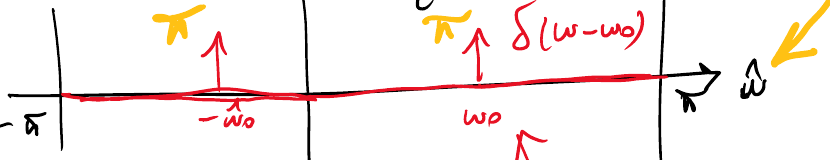
\includegraphics[scale=0.35]{immagini/lez20/spettroCoseno.jpg}
\end{figure}

Quindi lo spettro di un coseno ha solo una linea spettrale alla frequenze del coseno (come ci aspettiamo dalla formula di Eulero).

\section{Proprieta' DTFT della convoluzione}
E' una proprieta' molto importante, perche' ci permette di fare tante cose. Si utilizzano dei metodi spettrali, in cui un problema si cerca di risolverlo nel dominio spettrale perche' e' piu' facile.

Quello che ci dice questa proprieta' e' che la convoluzione di due segnali nel dominio nel tempo viene trasformata in un prodotto in quello delle frequenze (dopo aver trasformato i segnali tramite la DTFT):

\[\begin{split}
    &\mbox{TEMPO:  } z[n] = x[n] * y[n] = \sum_{k = -\infty}^{+\infty} x[n-k] y[k] \\
    &\mbox{Applicando la DTFT ai segnali:} \\
    &\mbox{FREQUENZE:  } Z(e^{j\hat{\omega}}) = X(e^j\hat{\omega}) \cdot Y(e^{j\hat{\omega}})
\end{split}\]

Dimostriamolo:

\[\begin{split}
    \mbox{DTFT} \{ z[n] \} &= \sum_{n=-\infty}^{+ \infty} z[n]e^{-j\hat{\omega}n} = \sum_{n=-\infty}^{+\infty} \sum_{k=-\infty}^{+\infty} x[n-k] y[k] e^{-j \hat{\omega}n} \\
    &= \sum_{k=-\infty}^{+\infty} y[k] \sum_{n=-\infty}^{+\infty} x[n-k] e^{-j \hat{\omega}n} \\
    &\mbox{Ricordando la proprieta' 5: DTFT } \{ x[n-k] \} = X(e^{j\hat{\omega}}) e^{-j\hat{\omega}k} \\
    &= \{ \sum_{k=-\infty}^{+\infty} y[k] e^{-j \hat{\omega}k} \} X(e^{j \hat{\omega}}) = Y(e^{j\hat{\omega}}) X(e^{j\hat{\omega}})
\end{split}\]

\section{Esercizio 1}
Facciamo ora degli esercizi per utilizzare le proprieta' della DTFT.
Come primo esercizio consideriamo come segnale una composizione lineare di delta:

\[
    x[n] = 2\delta[n+3] - \delta[n] - \delta[n-1] + 2\delta[n+1] + 5\delta[n-7]
\]

Ora utilizziamo la proprieta' di linearita' della DTFT ricordando inoltre che la DTFT di una delta e' 1 ed applichiamo anche la proprieta' del ritardo:

\[
    X(e^{j\hat{\omega}}) = 2 \cdot 1 e^{-j \hat{\omega}(-3)} -1 \cdot 1 e^{-j \hat{\omega}(0)} -1 \cdot 1 e^{-j \hat{\omega}(1)} + 2 \cdot 1 e^{-j \hat{\omega}(-1)} + 5 \cdot 1 e^{-j \hat{\omega}(7)}
\]

\section{Esericio 2}
Ora consideriamo come segnale il segnale rettangolo, che e' un segnale che vale 1 tra 0 ed $L-1$, e vale 0 altrimenti.

\begin{figure}[ht!]
    \centering
    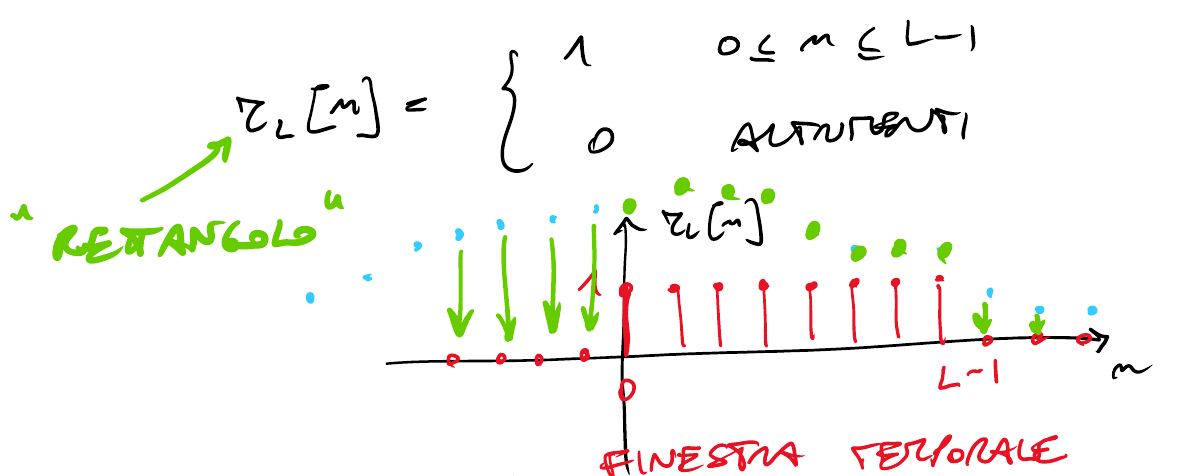
\includegraphics[scale=0.35]{immagini/lez21/es2Rettangolo.jpg}
\end{figure}

Moltiplicare per la finestra rettangolo per qualsiasi segnale significa focalizzarci su $L-1$ campioni. Vediamo ora la DTFT del segnale:

\[\begin{split}
    DTFT\{r_L [n]\} &= \sum_{n = -\infty}^{+\infty} r_L [n] e^{-j \hat{\omega}n} = \sum_{n=0}^{L-1}(e^{-j\hat{\omega}})^n \\
    &= \frac{1-q^L}{1-q} = \frac{1-e^{-j\hat{\omega}L}}{1-e^{-j\hat{\omega}}} \\
    &= e^{-j \hat{\omega} \frac{(L-1)}{2}} \frac{\sin \hat{\omega} \frac{L}{2}}{\sin\frac{\hat{\omega}}{2}} = R_L(e^{j\hat{\omega}})
\end{split}\]

Abbiamo ottenuto la forma di Dirichlet

\begin{figure}[ht!]
    \centering
    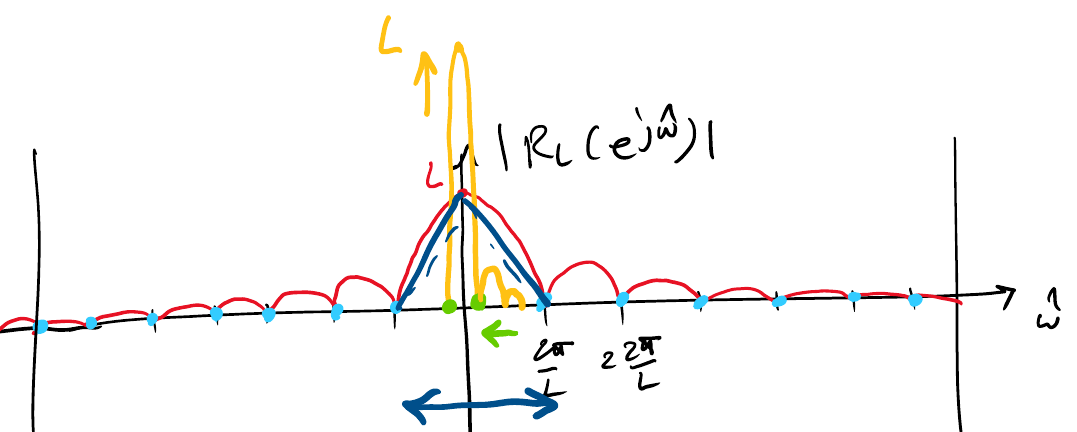
\includegraphics[scale=0.35]{immagini/lez21/es2ModuloRettangolo.jpg}
\end{figure}

Notiamo anche che se portiamo al limite l'area del primo lobo otteniamo una delta di dirac.

\section{Esempio 3}
Utilizziamo ora un segnale rettangolo per filtrare un segnale coseno :

\[\begin{split}
    x[n] &= \cos(\hat{\omega}_0 n) \leftrightarrow \pi \delta(\hat{\omega} - \hat{\omega}_0) + \pi \delta(\hat{\omega} + \hat{\omega}_0) \\
    \Tilde{x[n]} &= \cos(\hat{\omega}_0 n) r_L[n] \leftrightarrow \frac{1}{2} R_L (e^{j(\hat{\omega} - \hat{\omega}_0)}) + \frac{1}{2} R_L (e^{j(\hat{\omega} + \hat{\omega}_0)})
\end{split}\]

\begin{figure}[ht!]
    \centering
    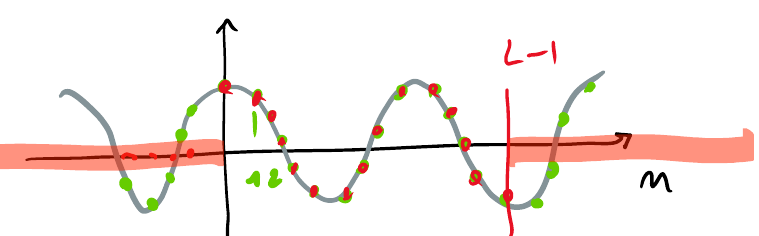
\includegraphics[scale=0.35]{immagini/lez21/filtraggioRettangolo.jpg}
\end{figure}

Ora calcoliamo la DTFT di questo segnale:

\[\begin{split}
    \mbox{DTFT}\{\Tilde{x[n]}\} &= \frac{1}{2} \mbox{DTFT} \{ e^{j \hat{\omega}_0 n} r_L[n] \} + \frac{1}{2} \mbox{DTFT} \{ e^{-j \hat{\omega}_0 n} r_L[n] \} \\
    &= \frac{1}{2} R_L(e^{j (\hat{\omega} - \hat{\omega}_0)}) + \frac{1}{2} R_L(e^{j (\hat{\omega} + \hat{\omega}_0)})
\end{split}\]

Tracciandone il grafico del modulo  e notiamo che quando ricostruiamo un segnale da uno troncato, otteniamo due lobi centrati dovo sono le componenti del coseno, nel caso in cui faccio tendere L all'infinito trovo esattamente la delta di Dirac.

\begin{figure}[ht!]
    \centering
    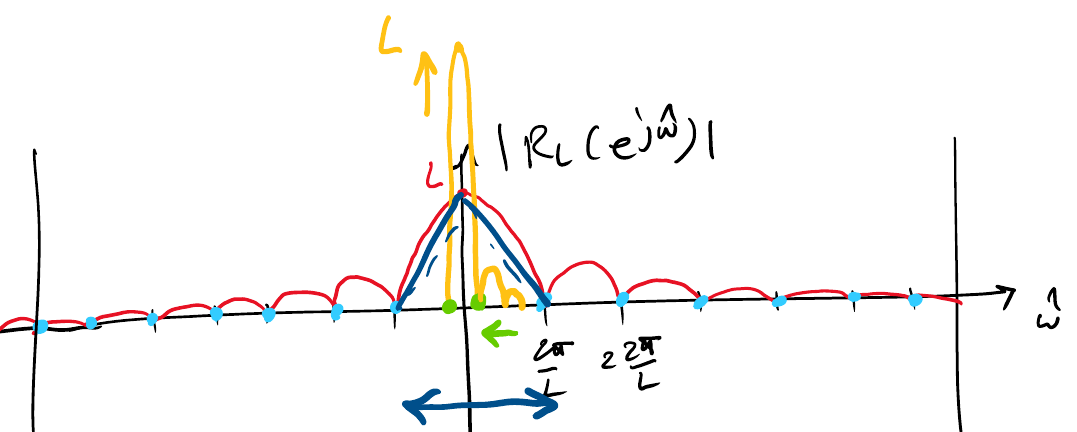
\includegraphics[scale=0.35]{immagini/lez21/es2ModuloRettangolo.jpg}
\end{figure}

\section{Teorema di Parseval (legge di conservazione) per segnali tempo discreti}
Prima di dare questo teorema diamo una definizione di \underline{energia di un segnale tempo discreto}: 

\begin{equation}
    E = \sum_{n= - \infty}^{+\infty} |x[n]|^2
\end{equation}

Diciamo che il teorema di Parseval passa dal dominio del tempo al dominio delle frequenze:

\begin{equation}
    E = \sum_{n= -\infty}^{+\infty} |x[n]|^2 = \frac{1}{2\pi} \int_{-\pi}^{\pi} |X(e^{j\hat{\omega}})|^2 d\hat{\omega}
\end{equation}

\begin{figure}[ht!]
    \centering
    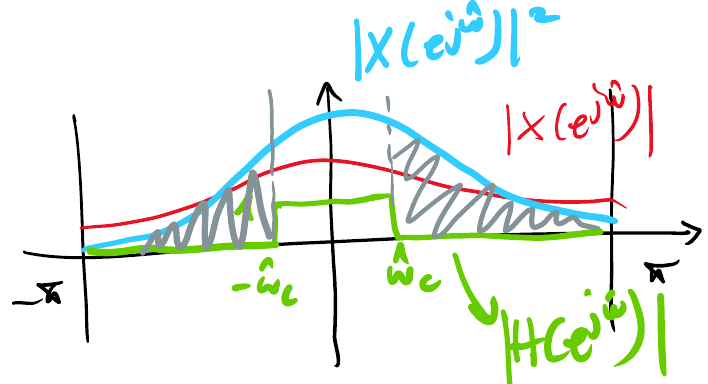
\includegraphics[scale=0.35]{immagini/lez21/teoremaParseval.jpg}
\end{figure}

Quello che succede in pratica e' che ci dice quant'e' l'energia associata a ciascuna delle frequenze del segnale.

Dimostriamolo per passi:

\subsection{Passo 1 dimostrazione}
Ribaltiamo la DTFT nel tempo e nelle frequenze:

\[\begin{split}
    \mbox{DTFT}\{x[-n]\} &= X()e^{-j \hat{\omega}} \\
    \mbox{DTFT}\{x^*[n]\} &= X^*(e^{-j\hat{\omega}})
\end{split}\]

\subsection{Passo 2 dimostrazione}
\[\begin{split}
    &\mbox{DTFT}\{x^*[n] * x[-n]\} = \\
    &\mbox{DTFT}\{x^*[n]\} \cdot \mbox{DTFT}\{x[-n]\} = \\
    &X^*(e^{-j\hat{\omega}}) \cdot X(e^{-j\hat{\omega}}) = 
    |X(e^{-j\hat{\omega}})|^2
\end{split}\]

Per un segnale reale e' la densita' spettrale di energia.

\subsection{Passo 2 dimostrazione}
\[\begin{split}
    x^*[n] * x[-n] &= \sum_{k = -\infty}^{+\infty} x*[n] x[-(n-k)] \\
    &= \sum_{k = -\infty}^{+\infty} x*[n] x[k-n] \\
    x^*[n] * y[n] &= \sum_{k = -\infty}^{+\infty} x[k] y[n-k]
\end{split}\]


\subsection{Passo 4 dimostrazione}

\[\begin{split}
    &\mbox{DTFT} \{x^*[n] * x[-n]\} = |X(e^{-j\hat{\omega}})|^2 \\
    &x^*[n] * x[-n] = \mbox{IDTFT} \{|X(e^{-j\hat{\omega}})|^2\} \\
\end{split}\]

Concludendo:

\begin{equation}
    \sum_{k = -\infty}^{+\infty} x^*[n] * x[k-n] = \frac{1}{2\pi} \int_{-\pi}^{\pi} |X(e^{-j\hat{\omega}})|^2 e^{j\hat{\omega}n} d\hat{\omega}
\end{equation}

Per i segnali reali togliamo i coniugati complessi ed $n=0$:

\[
    \sum_{k = -\infty}^{+\infty} |x[n]|^2 = \frac{1}{2\pi} \int_{-\pi}^{\pi} |X(e^{j\hat{\omega}})|^2 d\hat{\omega}
\]

\section{Matched Filter}

\begin{figure}[ht!]
    \centering
    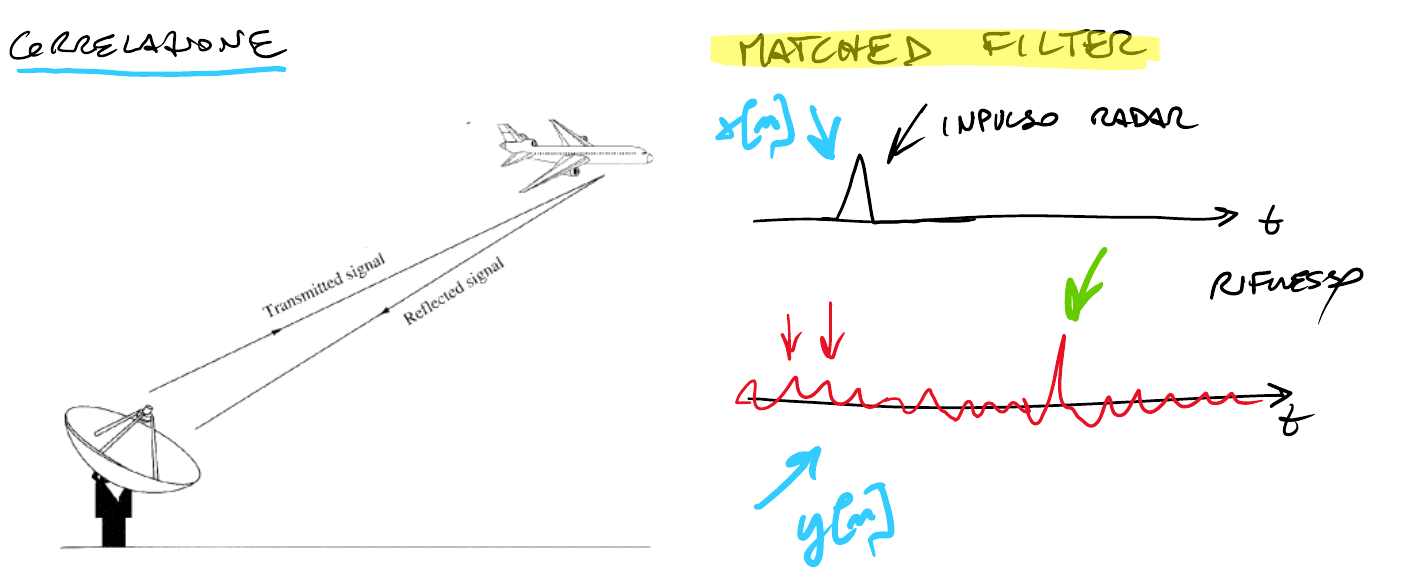
\includegraphics[scale=0.35]{immagini/lez22/matchedFilter.jpg}
\end{figure}

Il matched filter serve per localizzare occorrenze di un segnale in un altro (in presenza di rumore). Calcolando la (cross-)correlazione di un template o maschera con il segnale. La correlazione e' massima quando sono identici.

\section{Precisazione cambio di variabile}
Quando ricostruiamo un segnale tramite la IDTFT possiamo farlo nel mondo del tempo utilizzando l'integrale tra $-\pi$ e $\pi$, oppure possiamo farlo nel mondo delle frequenze cambiando variabile:

\[\begin{split}
    x[n] &= \frac{1}{2\pi} \int_{-\pi}^{\pi} X(e^{j\hat{\omega}}) e^{j\hat{\omega}n} d\hat{\omega} \\
    \hat{f} &= \frac{\hat{\omega}}{2\pi} \Rightarrow d\hat{f} = \frac{d\hat{\omega}}{2\pi} \\
    &= \frac{1}{\cancel{2\pi}} \int_{\frac{-\pi}{2\pi} = -\frac{1}{2}}^{\frac{\pi}{2\pi} = \frac{1}{2}} X(e^{j2\pi\hat{f}}) e^{j2\pi\hat{f}n} \cancel{2\pi} d\hat{f}
\end{split}\]

\section{Risposta in frequenza e DTFT}
Torniamo a parlare della risposta in frequenza, sappiamo che l'uscita di un sistema LTI e' la convoluzione tra il segnale in ingresso e la sua risposta all'impulso.
Dato che sappiamo che la DTFT se esiste e' unica, allora :

\[\begin{split}
    \mbox{DTFT}\{y[n]\} &= \mbox{DTFT}\{x[n] * h[n]\} \\
    Y(e^{j\hat{\omega}} &= X(e^{j\hat{\omega}}) \cdot \mbox{DTFT}\{h[n]\} \\
    \mbox{DTFT}\{h[n]\} &= \sum_{n=-\infty}^{+\infty} h[n] e^{-j \hat{\omega} n_0} = H(e^{j\hat{\omega}})
\end{split}\]

Abbiamo quindi trovato un terzo modo per vedere la risposta in frequenze che e' la DTFT del sistema e possiamo trovarla dal rapporto tra la DTFT dell'uscita del sistema e la DTFT dell'ingresso del sistema:

\[\begin{split}
    Y(e^{j\hat{\omega}} &= X(e^{j\hat{\omega}}) \cdot H(e^{j\hat{\omega}}) \\
    H(e^{j\hat{\omega}}) &= \frac{Y(e^{j\hat{\omega}}}{X(e^{j\hat{\omega}})}
\end{split}\]

\section{Filtraggio (LTI) nel tempo vs frequenze}

\begin{figure}[ht!]
    \centering
    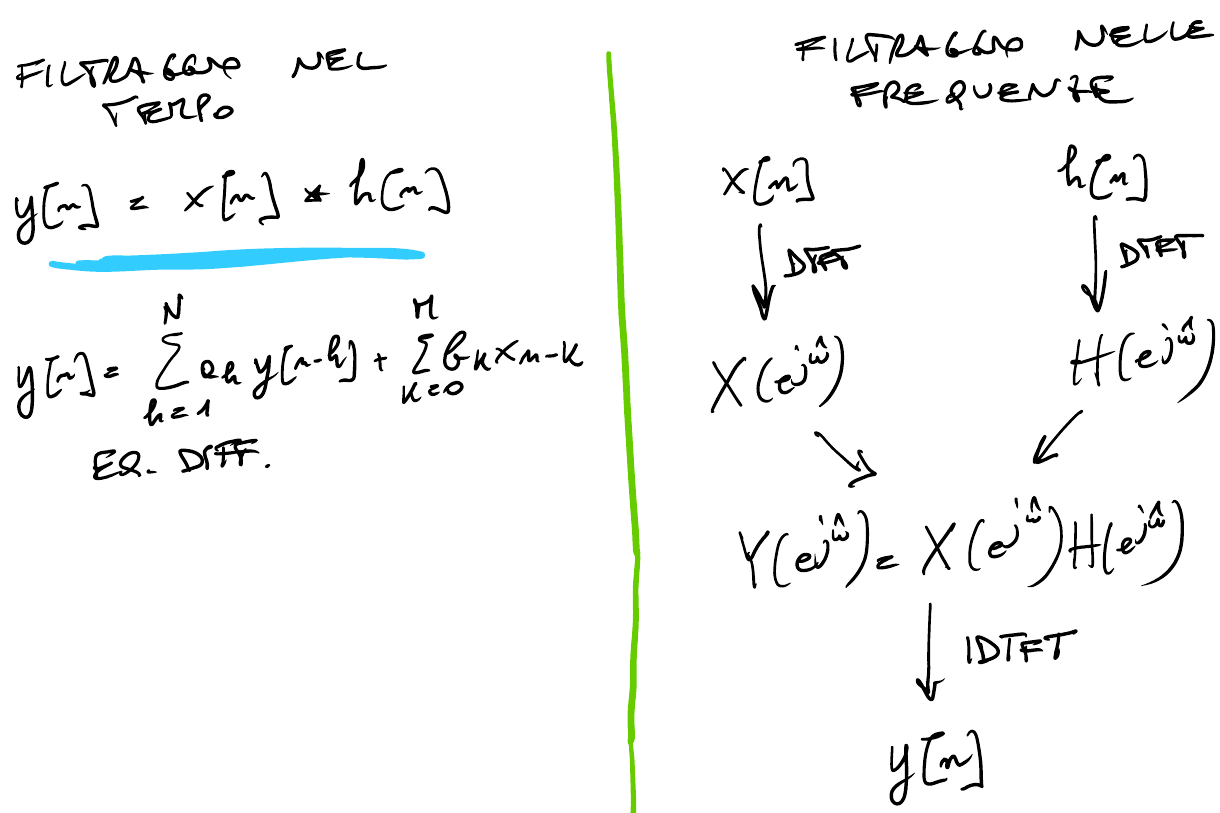
\includegraphics[scale=0.35]{immagini/lez22/filtraggioTempoFrequenze.jpg}
\end{figure}

Da questa chiarificazione notiamo che a volte puo' essere piu' semplice portarsi nel dominio delle frequenze per fare il filtraggio, in modo tale che la convoluzione si trasformi in una moltiplicazione.

Possiamo ancora ragionare sul filtraggio LTI, posso calcolare la DTFT di un segnale ed ottenere il modulo della DTFT, poi dato che voglio filtrare moltiplico quel modulo per il modulo della risposta all'impulso del filtro che mi interessa (nel nostro caso un filtro passa basso), faccio una moltiplicazione punto punto ed ottengo il modulo dell'uscita del sistema.

\begin{figure}[ht!]
    \centering
    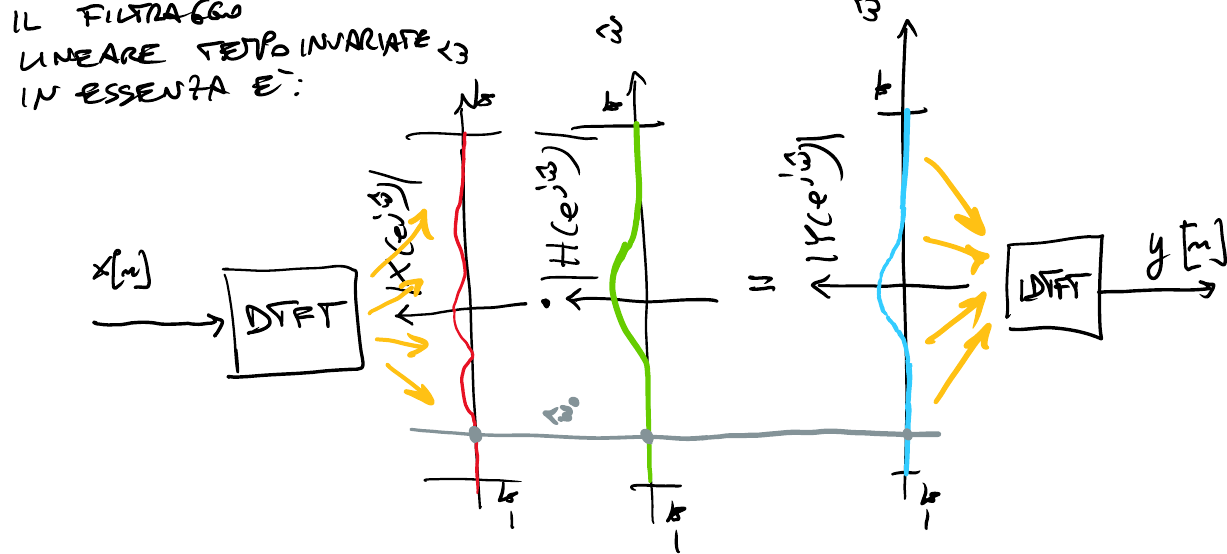
\includegraphics[scale=0.35]{immagini/lez22/filtraggioLTI.jpg}
\end{figure}

\section{Un primo esempio di sistema LIT IIR}
Fino ad ora abbiamo considerato sistemi FIR. Ora sappiamo anche manipolare sistemi LTI con risposta all'impulso infinita.
Vediamo un primo esempio di sistema LTI IIR:

\[\begin{split}
    y[n] &= \frac{1}{2} y[n-1] + x[n] \\
    x[n] &= \delta[n]
\end{split}\]

Notiamo subito che c'e' la parte autoregressiva quindi e' probabile che il sistema sia IIT, vogliamo trovare l'output del sistema.

Calcoliamo l'output del sistema nei punti in cui e' diverso da 0:

\[\begin{split}
    y[-2] &= h[-2] = 0 \\
    y[-1] &= h[-1] = 0 \\
    y[0] &= h[0] = 1 = (\frac{1}{2})^0\\
    y[1] &= \frac{1}{2} \cdot 1 + 0 = \frac{1}{2} = (\frac{1}{2})^1\\
    y[2] &= \frac{1}{2} \cdot \frac{1}{2} + 0 = \frac{1}{4} = (\frac{1}{2})^2\\
    y[3] &= \frac{1}{2} \cdot \frac{1}{4} + 0 = \frac{1}{8} = (\frac{1}{2})^3\\
\end{split}\]

Da questi punti notiamo che il segnale in uscita ha un andamento del tipo:

\[
    y[n] = h[n] = (\frac{1}{2})^n u[n]
\]

\begin{figure}[ht!]
    \centering
    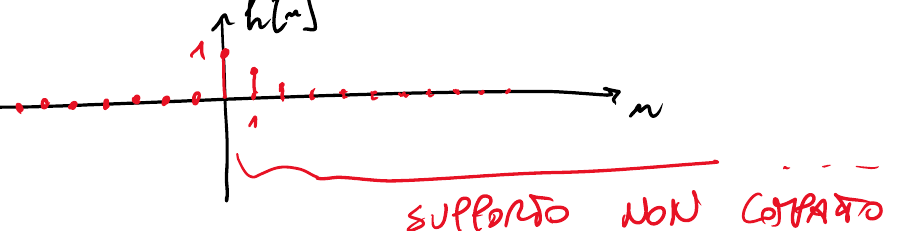
\includegraphics[scale=0.35]{immagini/lez22/es1.jpg}
\end{figure}

Ora per calcolare la risposta in frequenza utilizziamo le coppie di DTFT che abbiamo usato in precedenza per vedere se possiamo ricondurci a qualcuna di esse:

\[
    H(e^{j\hat{\omega}}) = \sum_{n=-\infty}^{+\infty} h[n] e^{-j\hat{\omega}n} = DTFT\{h[n\} = \frac{1}{1 - \frac{1}{2} e^{-j\hat{\omega}}}
\]

Abbiamo risolto questo esercizio in 3 passaggi, siamo partiti dall'equazione alle differenze, abbiamo trovato la risposta all'impulso ed infine abbiamo calcolato la risposta in frequenza, proviamo a farlo in un passaggio solo passando direttamente dall'equazione alle differenze alla risposta in frequenza.

\begin{figure}[ht!]
    \centering
    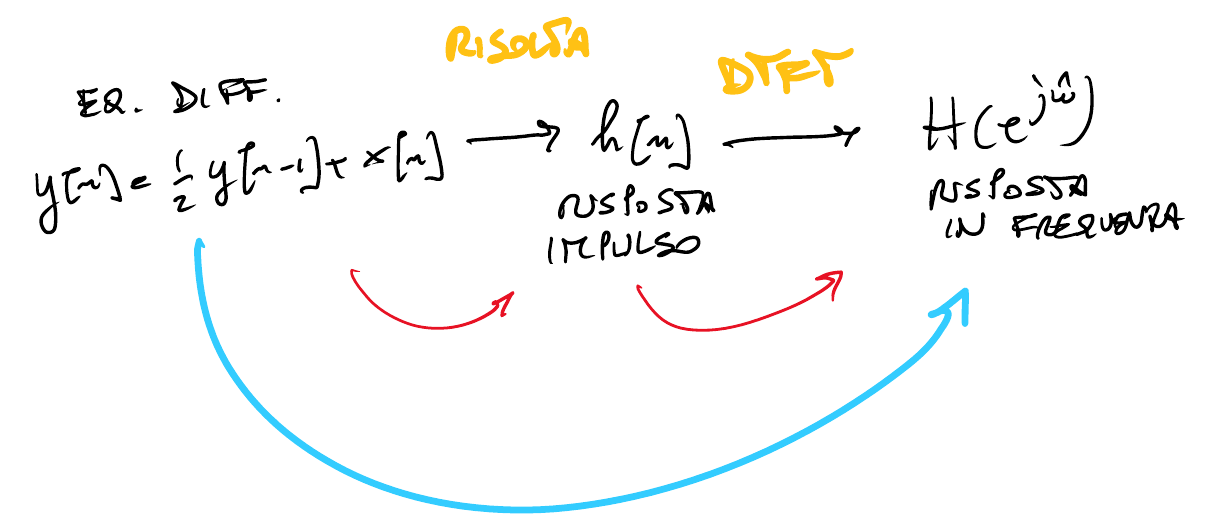
\includegraphics[scale=0.35]{immagini/lez22/es13passaggi.jpg}
\end{figure}

\[\begin{split}
    y[n] &= \frac{1}{2} y[n-1] + x[n] \rightarrow \mbox{ usiamo la proprieta' dell'unicita' della DTFT} \\
    \mbox{DTFT}\{y[n]\} &= \mbox{DTFT}\{\frac{1}{2} y[n-1] + x[n]\} \rightarrow \mbox{ usiamo la proprieta' di linearita'} \\ 
    Y(e^{j\hat{\omega}}) &= \frac{1}{2} \mbox{DTFT}\{y[n-1]\} + \mbox{DTFT}\{x[n]\} \rightarrow \mbox{ ora applichiamo la proprieta' del ritardo} \\
    Y(e^{j\hat{\omega}}) &= \frac{1}{2} Y(e^{j\hat{\omega}}) e^{-j \hat{\omega}1} + X(e^{j\hat{\omega}}) \\
    Y(e^{j\hat{\omega}}) (1 - \frac{1}{2} e^{-j\hat{\omega}}) &= X(e^{j\hat{\omega}}) \\
    \frac{Y(e^{j\hat{\omega}})}{X(e^{j\hat{\omega}})} &= \frac{1}{1-\frac{1}{2}e^{-j\hat{\omega}}} 
\end{split}\]

Lo stesso ragionamento lo possiamo fare per qualunque equazione alle differenze:

\[\begin{split}
    y[n] &= \sum_{h = -N_1, h \neq 0}^{N_2} ah y[n-h] + \sum_{h = -M_1, h \neq 0}^{M_2} bk x[n-k] \\
    &\mbox{Proprieta' di unicita'} \\
    \mbox{DTFT} \{y[n]\} &= \mbox{DTFT} \{\sum_{h = -N_1, h \neq 0}^{N_2} ah y[n-h] + \sum_{h = -M_1, h \neq 0}^{M_2} bk x[n-k]\} \\
    &\mbox{Proprita' di linearita'}\\
    Y(e^{j\hat{\omega}}) &= \sum_{h = -N_1, h \neq 0}^{N_2} ah \mbox{DTFT} \{y[n-h]\} + \sum_{h = -M_1, h \neq 0}^{M_2} bk \mbox{DTFT} \{x[n-k]\} \\
    &\mbox{Proptieta' del ritardo} \\
    Y(e^{j\hat{\omega}}) \{1- \sum_{h = -N_1, h \neq 0}^{N_2} ah e^{-j\hat{\omega}h}\} &= X(e^{j\hat{\omega}}) \{1- \sum_{h = -M_1, h \neq 0}^{M_2} bk e^{-j \hat{\omega}k}\} \\
    \frac{Y(e^{j\hat{\omega}})}{X(e^{j\hat{\omega}})} &= \frac{\sum_{h = -M_1, h \neq 0}^{M_2} bk e^{-j \hat{\omega}k}}{\sum_{h = -N_1, h \neq 0}^{N_2} ah e^{-j\hat{\omega}h}}
\end{split}\]

\section{Esercizio}
Dato un equazione alle differenze di un sistema LTI:

\[
    y[n] = \frac{9}{10} y[n-1] + \frac{1}{20} x[n] + \frac{1}{20} x[n-1]
\]

calcolare la risposta in frequenza e poi la risposta all'impulso.
Cominciamo calcolando la risposta in frequenza usando le proprieta' di unicita', linearita' e del ritardo come abbiamo fatto fino ad adesso:

\[\begin{split}
    &Y(e^{j\hat{\omega}}) = \frac{9}{20} Y(e^{j\hat{\omega}})e^{-j\hat{\omega} 1} + \frac{1}{20} X(e^{j\hat{\omega}}) + \frac{1}{20} X(e^{j\hat{\omega}})e^{-j\hat{\omega}1} \\
    &Y(e^{j\hat{\omega}}) \{1-\frac{9}{10}e^{-j\hat{\omega}}\} = X(e^{j\hat{\omega}})\{\frac{1}{20} + \frac{1}{20}e^{-j\hat{\omega}}\} \\
    &\frac{Y(e^{j\hat{\omega}})}{X(e^{j\hat{\omega}})} = \frac{\frac{1}{20}(1+e^{-j\hat{\omega}})}{1-\frac{9}{10}e^{-j\hat{\omega}}} = H(e^{j\hat{\omega}})
\end{split}\]

Per trovare la risposta all'impulso dobbiamo calcolare $h[n] = IDTFT\{H(e^{j\hat{\omega}}\}$, per farlo andiamo a vedere le proprieta' e le coppie di DTFT per vedere se possiamo riscrivere H in modo da ricondurci a delle coppie note:

\[\begin{split}
    H(e^{j\hat{\omega}}) &= \frac{1}{20} \cdot \frac{1}{1-\frac{9}{10}e^{-j\hat{\omega}}} + \frac{1}{20}e^{e^{-j\hat{\omega}}} \cdot \frac{1}{1-\frac{9}{10} e^{-j\hat{\omega}}} \\
    h[n] &= \frac{1}{20} \cdot (\frac{9}{10})^n u[n] + \frac{1}{20} \cdot (\frac{9}{10})^{n-1} u[n-1]
\end{split}\]

\section{DFT}
\begin{figure}[ht!]
    \centering
    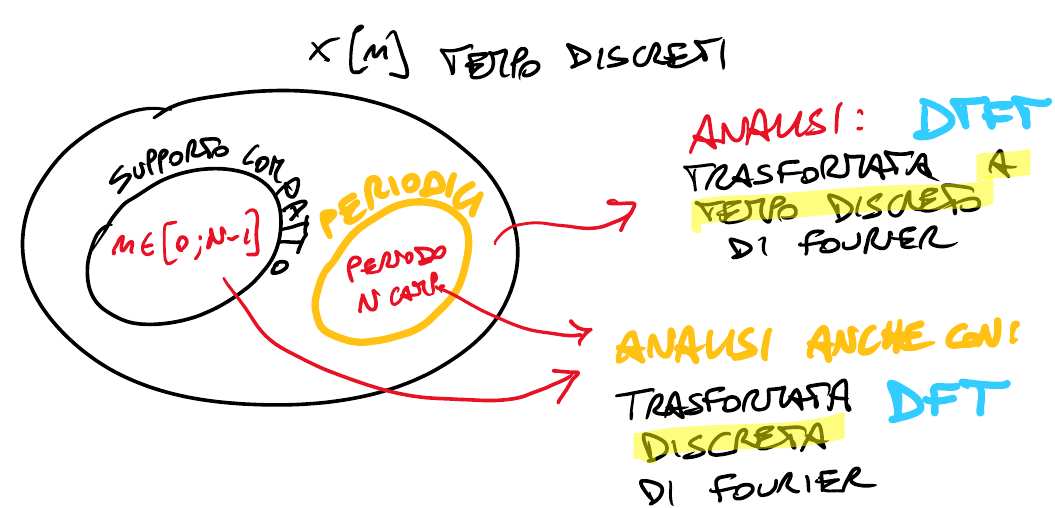
\includegraphics[scale=0.35]{immagini/lez23/segnaliDFT.jpg}
\end{figure}

In realta' i sottoinsiemi di segnali che ci interessano, ovvero i segnali a supporto compatto e/o periodici, possono essere analizzati tramite un operatore piu' comodo della DTFT, la \underline{trasformata discreta di Fourier DFT}.

Sappiamo che la DTFT di un segnale e':

\[
    \mbox{DTFT}\{x[n]\} = X(e^{j\hat{\omega}}) = \sum_{n = \cancel{-\infty} 0 }^{\cancel{+\infty} N-1} x[n] e^{-j\hat{\omega}n}
\]

Dato che stiamo prendendo in considerazione solo segnali a supporto compatto possiamo ridurre la sommatoria ad $n \in [0, N-1]$, inoltre possiamo discretizzare la frequenza, ovvero prendiamo un numero limitato di campioni perche' se nella DTFT $\hat{\omega} \in \mathbf{R} (-\pi; +\pi]$, nella DFT consideriamo $\hat{\omega}_k = \frac{2\pi}{N}\cdot k \rightarrow k\in[0; N-1]$. Quindi concludendo la DFT di un segnale e':

\begin{equation}
    \mbox{DFT}\{x[n]\} X_{[k]} = \sum_{n=0}^{N-1} x[n] e^{-j\frac{2\pi}{N} \cdot kn}
\end{equation}

\begin{figure}[ht!]
    \centering
    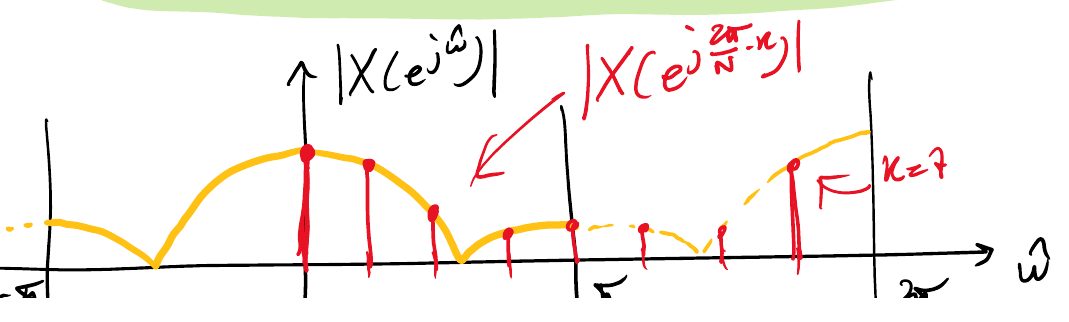
\includegraphics[scale=0.35]{immagini/lez23/moduloDFT.jpg}
\end{figure}

Esiste anche una formula di sintesi la IDFT:

\[
\mbox{IDFT}\{x_{[k]}\} = \frac{1}{N} \sum_{n=0}^{N-1} x[n] e^{j\frac{2\pi}{N} \cdot kn}
\]

\medskip
\medskip
\medskip
\medskip
\medskip
\medskip
\medskip
\medskip
\medskip
\medskip
\medskip
\medskip
\medskip
\medskip
\medskip
\medskip
\medskip
\medskip
\medskip
\medskip
\medskip
\medskip
\medskip
\medskip
\medskip
\medskip
\medskip
\medskip
\medskip
\medskip
\medskip
\medskip
\medskip
\medskip
\medskip
\medskip
\medskip
\medskip
\medskip
\medskip
\medskip
\medskip
\medskip
\medskip
\medskip
\medskip
\medskip
\medskip
\medskip
\medskip
\medskip
\medskip
\medskip
\medskip
\medskip
\medskip
\medskip
\medskip
\medskip
\medskip
\medskip
\medskip
\medskip
\medskip
\medskip
\medskip
\medskip
\medskip
\medskip
\medskip
\medskip
\medskip
\medskip
\medskip
\medskip
\medskip
\medskip
\medskip
\medskip
\medskip
\medskip
\medskip
\medskip
\medskip
\medskip
\medskip
\medskip
\medskip
\medskip
\medskip
\medskip
\medskip
\medskip

\subsection{Esercizio}

\begin{figure}[ht!]
    \centering
    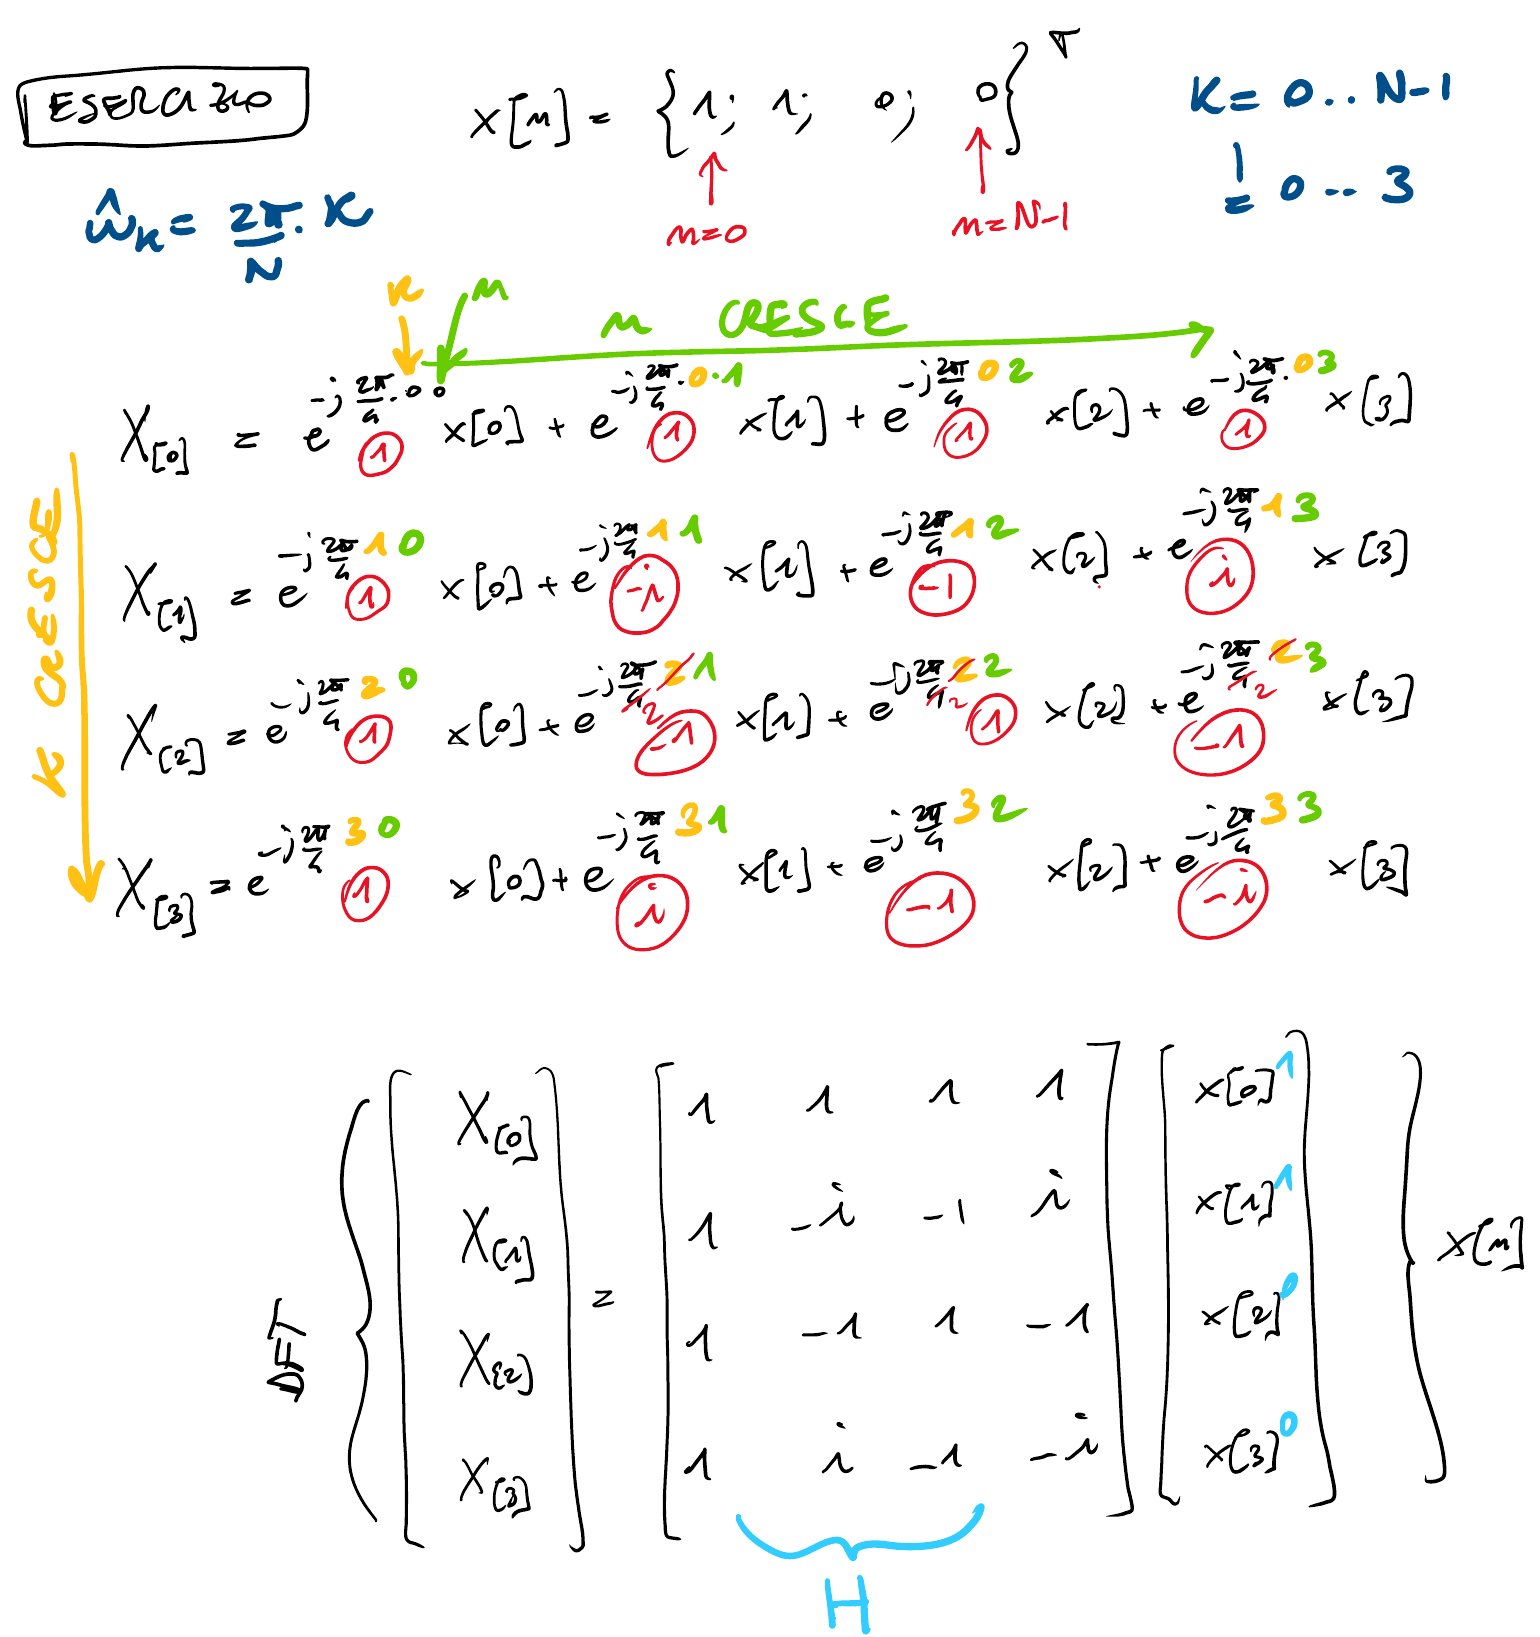
\includegraphics[scale=0.35]{immagini/lez23/esercizio.jpg}
\end{figure}


Abbiamo fatto un esercizio per vedere come funziona la DFT per un vettore di 4 elementi, quindi sappiamo che in questo caso $k=3$ ed N pure, quello che abbiamo fatto e' stato calcolare elemento per elemento la DFT sostituendo opportunamente k ed N nella formula. Successivamente abbiamo visto quanto valgono gli esponenziali complessi (i numeri cerchiati in rosso), ed abbiamo notato che quindi quello che succede e' come se moltiplicassimo il segnale per una matrice H, ed i punti che otteniamo sono:

\[\begin{split}
    X_[0] = 2 \rightarrow \hat{\omega}_{k=0} = \frac{2\pi}{4} \cdot 0 = 0 \\
    X_[1] = 1 - i \rightarrow \hat{\omega}_{k=1} = \frac{2\pi}{4} \cdot 1 = \frac{\pi}{2} \\
    X_[2] = 0 \rightarrow \hat{\omega}_{k=2} = \frac{2\pi}{4} \cdot 2 = \pi \\
    X_[3] = 1 + i \rightarrow \hat{\omega}_{k=3} = \frac{2\pi}{4} \cdot 3 = \frac{3}{2}\pi \\
\end{split}\]

\begin{figure}[ht!]
    \centering
    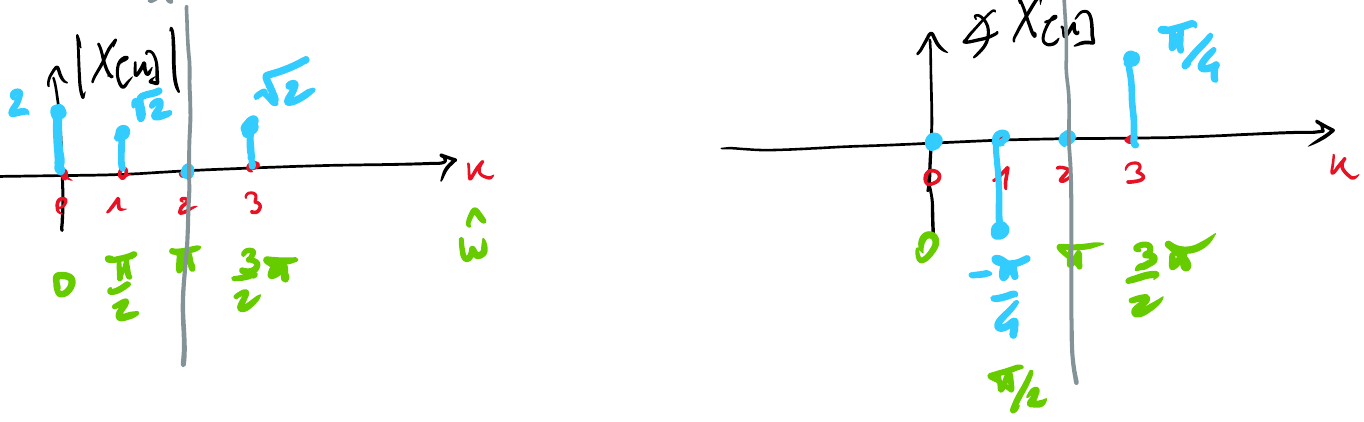
\includegraphics[scale=0.35]{immagini/lez23/moduloFaseEsercizio.jpg}
\end{figure}

Tracciando il grafico del modulo e della fase notiamo che non sono simmetrici, questo perche' abbiamo considerato la simmetria fuori dall'alias principale.

Quindi concludendo possiamo dire che la DFT di un segnale (vettore) e' il segnale stesso moltiplicato per la matrice H:

\[
    \mbox{DFT: } X_[k] = H x[n]
\]

di conseguenza possiamo riscrivere la IDFT come il segnale moltiplicato per la matrice coniugata (coniugato di elemento per elemento della matrice) e trasposta (ruotata sulla diagonale):

\[
    \mbox{IDFT: } x[n] = H^{-1} X_[k] = \frac{1}{N}(H^*)^T \cdot X_[k]
\]

Per avere in riscontro di quello fatto adesso in questo esercizio, calcoliamo la DTFT del vettore per vedere se troviamo gli stessi punti:

\[\begin{split}
    \mbox{DTFT}\{[1100]\} &= 1 + e^{-j\hat{\omega}} = 2e^{-j\frac{\hat{\omega}}{2}} (\frac{e^{j\frac{\hat{\omega}}{2}} + e^{j\frac{\hat{\omega}}{2}}}{2}) \\
    &= 2e^{-j\frac{\hat{\omega}}{2}} \cos \frac{\hat{\omega}}{2}
\end{split}\]

Tracciamo il grafico del modulo e della fase:

\begin{figure}[ht!]
    \centering
    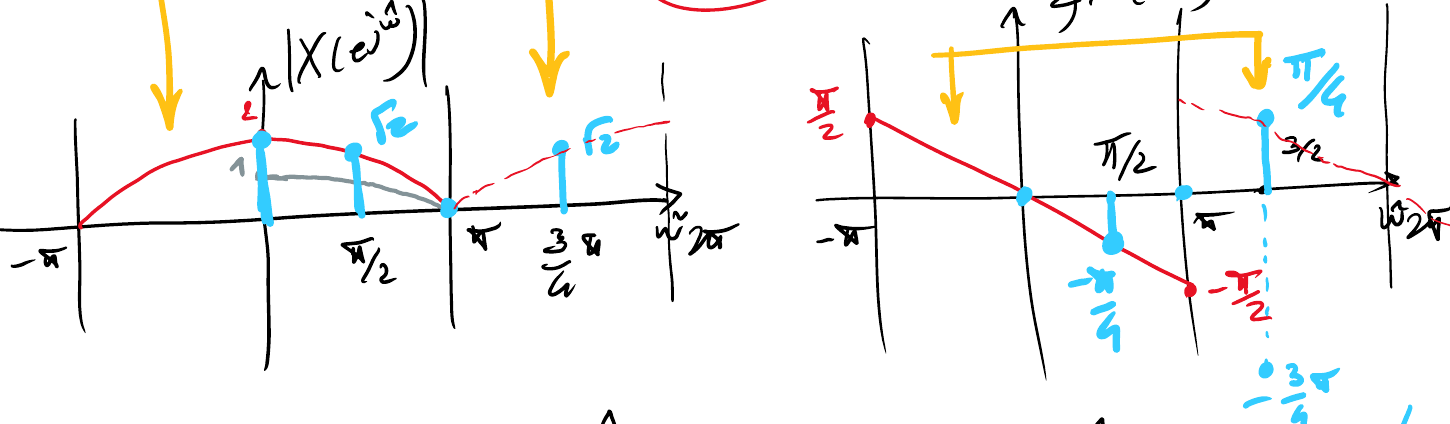
\includegraphics[scale=0.35]{immagini/lez23/moduloFaseEs1.jpg}
\end{figure}

Ora calcoliamo la DTFT per ogni punto del vettore per vedere se ottengo gli stessi punti che abbiamo trovato prima:

\[\begin{split}
    \hat{\omega} &= 0 \rightarrow X(e^{j\hat{\omega}}) = 2 \\
    \hat{\omega} &= \frac{\pi}{2} \rightarrow X(e^{j\hat{\omega}}) = 2cos\frac{\pi}{4} e^{-j\frac{\pi}{4}} \\
    \hat{\omega} &= \pi \rightarrow X(e^{j\hat{\omega}}) = 2cos\frac{\pi}{2} e^{-j\frac{\pi}{2}} \\
    \hat{\omega} &= \frac{3}{2}\pi \rightarrow X(e^{j\hat{\omega}}) = 2cos\frac{3}{4} \pi e^{-j\frac{3}{4}\pi} \\
\end{split}\]

\section{Proprieta' della DFT}
Vediamo le varie proprieta' della DFT come abbiamo fatto in precedenza per la DTFT

\subsection{Proprieta' 1: DFT periodica di N punti}
A differenze della DTFT che era periodica di $2\pi$ la DFT e' periodica di N punti:

\[\begin{split}
    &k \rightarrow \frac{2\pi}{N} \cdot k = \hat{\omega} \\
    X_[k] &= \sum_{n=0}^{N-1} x[n] e^{-j \frac{2\pi}{N}\cdot kn} \\
    X_[k+n] &= \sum_{n=0}^{N-1} x[n] e^{-j \frac{2\pi}{N}(k+N)n} \\
    &= \sum_{n=0}^{N-1} x[n]e^{-j \frac{2\pi}{N} \cdot kn} \cdot \cancel{e^{-j \frac{2\pi}{\cancel{N}}\cdot n \cancel{N}}} \\
    X_[k+n] &= X_[k]
\end{split}\]

\subsection{Propritea' 2: DFT e' simmetrica coniugata se $x[n] \in \mathbf{R}$ }

La DTFT e' simmetrica coniugata se il segnale e' reale, il che vuol dire che $X(e^{-j\hat{\omega}}) = X^*(e^{j\hat{\omega}})$, quindi avevamo una simmetria dei campioni che si "ribaltavano" sull'asse y. Mentre con la DFT abbiamo una simmetria ma su $\pi$.

Quindi quello che succede per il modulo e' che ho un campione iniziale $k=0$ che e' centrato sull'asse y, poi ho una serie di campioni che vengono copiati uguali e ribaltati sul campione centrale $k = \frac{N}{2} + 1$. Mentre con la fase ho sempre un campione iniziale ed uno centrale, ed i campioni tra quello iniziale e centrale vengono ribaltati e copiati cambiati di segno.
Notiamo che il campione centrale esiste solamente se N e' pari, inoltre facciamo attenzione al fatto che il campione iniziale $k=0$ ed il campione centrale in $\pi$ DEVONO essere numeri Reali.

\begin{figure}[ht!]
    \centering
    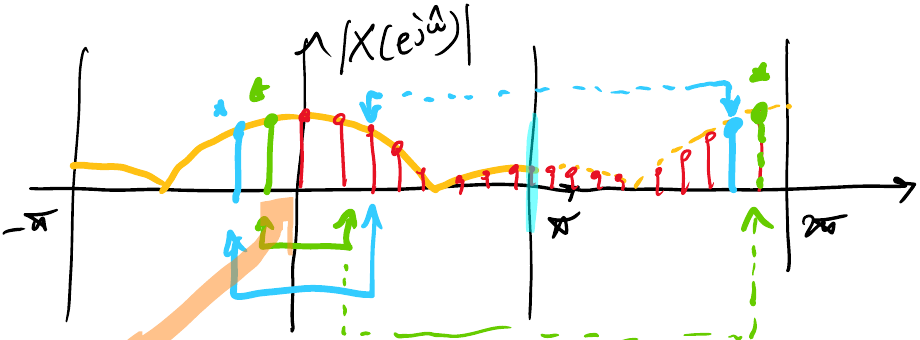
\includegraphics[scale=0.35]{immagini/lez24/DFTsimmetricaConiugata.jpg}
\end{figure}

\begin{figure}[ht!]
    \centering
    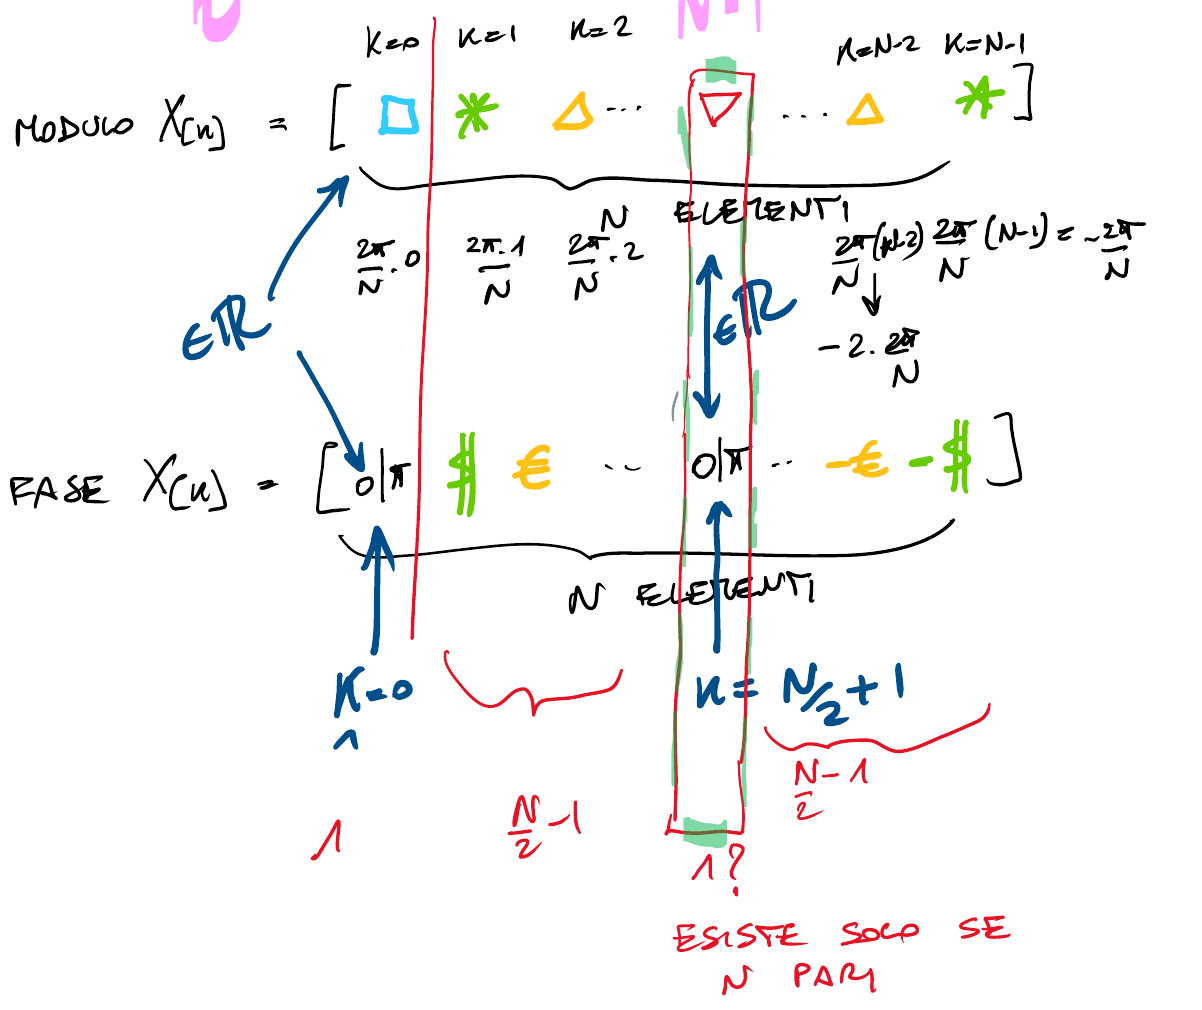
\includegraphics[scale=0.30]{immagini/lez24/DTFesempio.jpg}
\end{figure}


\subsubsection{Esercizio}
Facciamo un esercizio per vedere data una DFT se il segnale era reale.
Abbiamo un vettore di 8 elementi, quindi N e' pari di conseguenza avremo il campione centrale a $\pi$ che nel nostro caso e' il posizione 4 del vettore ed e' uguale a $1+i$.
Ora passo passo verifichiamo che le condizioni date prima sono verificate, il campione in posizione $k=0$ e quello centrale in posizione $\pi$ sono due numeri reali, quindi va bene. Poi verifichiamo che le varie coppie siano coniugati complessi, e vediamo subito che la prima coppia (ovvero l'elemento in posizione 1 e l'ultimo, quello in posizione 7) non sono coniugati complessi. Quindi possiamo subito concludere che il segnale non era reale.

\begin{figure}[ht!]
    \centering
    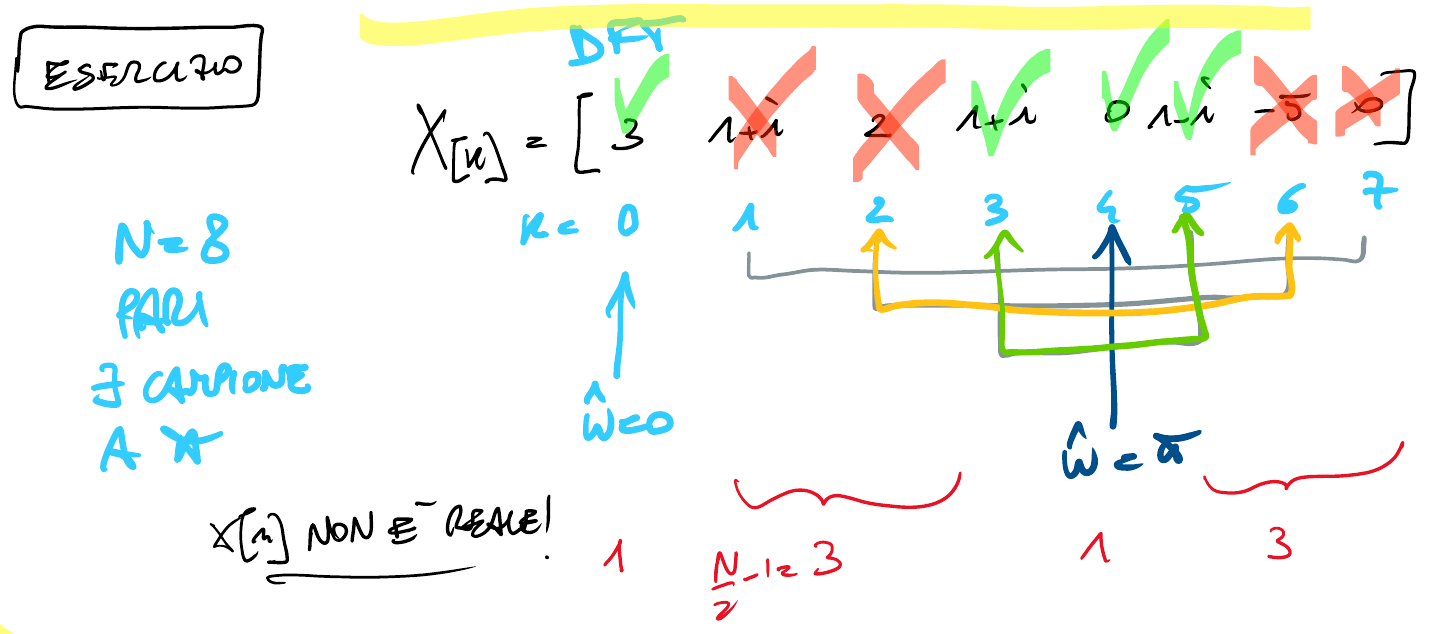
\includegraphics[scale=0.35]{immagini/lez24/esercizioDFT.jpg}
\end{figure}

\subsection{Proprieta' 4: DFT e' unica}
La DFT, che esiste sempre, e' unica solo per segnali periodici. Il segnale $x[n]$ a supporto compatto $[0; N-1]$ ha la stessa DFT di un segnale periodico $X_p[n]$ di periodo N avente periodo base uguale a $x[n]$ per $n \in [0; N-1]$.

\begin{figure}[ht!]
    \centering
    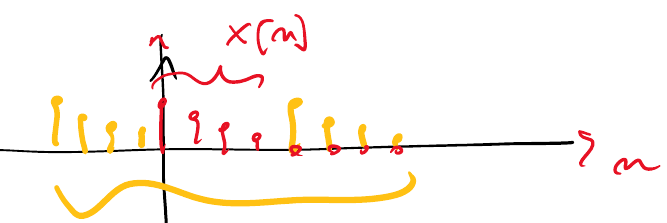
\includegraphics[scale=0.35]{immagini/lez24/prop4.jpg}
\end{figure}

\subsection{Proprieta' 5: ritardo temporale}
Ricordiamo la proprieta' del ritardo temporale per la DTFT:

\[
    \mbox{DTFT} x[n-n_0] \leftrightarrow X(e^{j\hat{\omega}})e^{-j\hat{\omega}n_0}
\]

Vediamo cosa succede se ritardiamo la DFT, partiamo ricordando com'e' fatta la DFT di un segnale:

\[
    x[n] = \frac{1}{N} \sum_{k=0}^{N-1} X_[k]e^{-j \frac{2\pi}{N} \cdot kn}
\]

\begin{figure}[ht!]
    \centering
    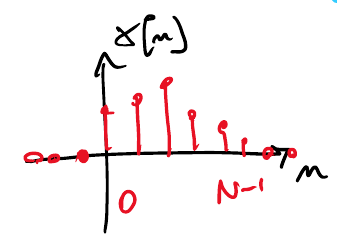
\includegraphics[scale=0.35]{immagini/lez24/x[n]Prop5.jpg}
\end{figure}

ora ritardiamo il segnale sostituendo $n+N$ ad n:

\[\begin{split}
    x[n+N] &= \frac{1}{N} \sum_{k=0}^{N-1} X_[k]e^{-j \frac{2\pi}{N} (n+N) \cdot k}\\
    &= \sum_{n=0}^{N-1} x[n]e^{-j \frac{2\pi}{N} \cdot kn} \cdot \cancel{e^{-j \frac{2\pi}{\cancel{N}}\cdot n \cancel{N}}} \\
    X_[n+N] &= X_[n]
\end{split}\]

Quindi attenzione perche' la ricostruzione rende periodico il segnale. La $x[n]$ corrisponde sia alla DFT di un segnale a supporto compatto che a quella di uno periodico.

\begin{figure}[ht!]
    \centering
    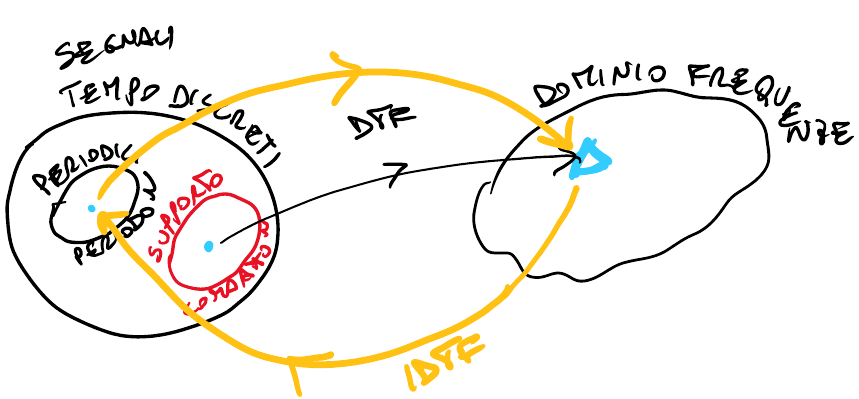
\includegraphics[scale=0.35]{immagini/lez24/DFTperiodica.jpg}
\end{figure}

Questo pero' e' un problema, in quanto se trasliamo un segnale che e' stato ricostruito e reso periodico, nell'alias principale entrano dei campioni che generano rumore e non vorremmo:

\begin{figure}[ht!]
    \centering
    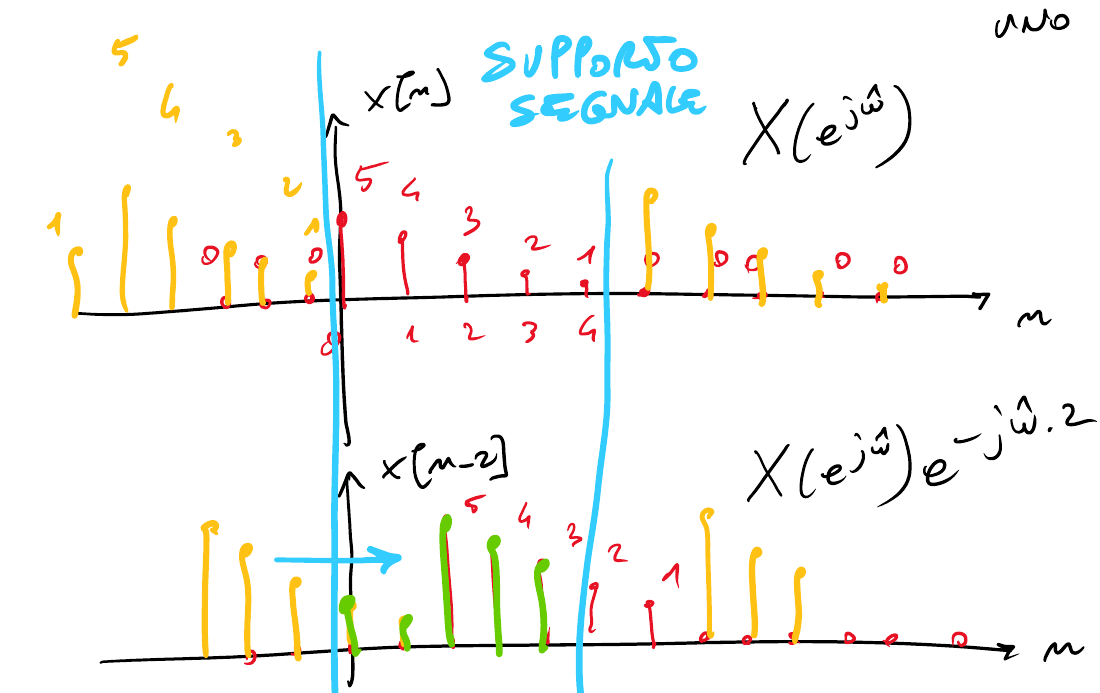
\includegraphics[scale=0.35]{immagini/lez24/DFTaliasSecondari.jpg}
\end{figure}

\begin{figure}[ht!]
    \centering
    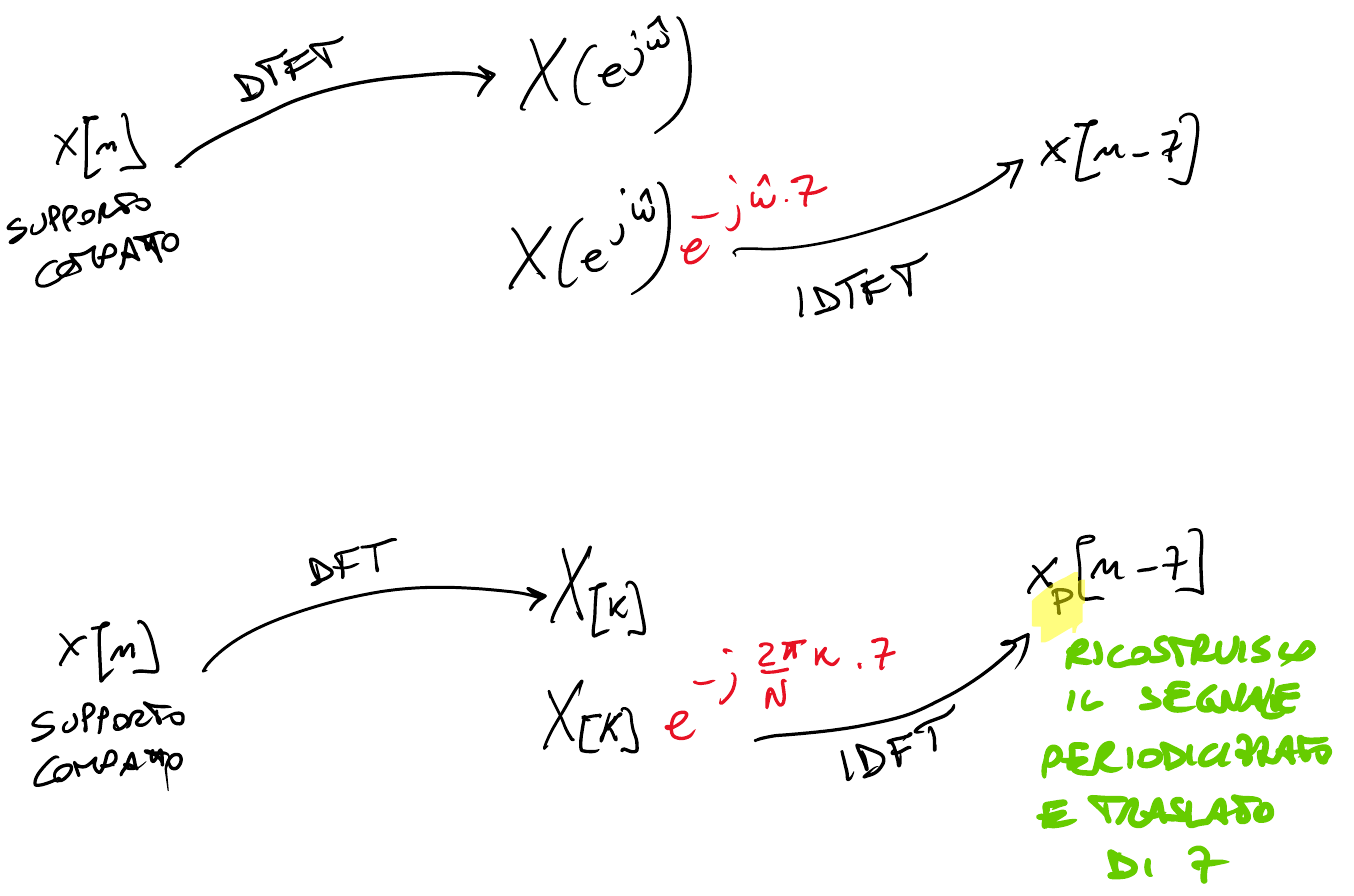
\includegraphics[scale=0.35]{immagini/lez24/DFTIDTFT.jpg}
\end{figure}


\subsection{Proprieta' 6: convoluzione}
La convoluzione la usiamo spesso per filtrare un segnale, ma vale anche tra due segnali.
Sappiamo che per trvare l'uscita di un sistema LTI dobbiamo fare la convoluzione tra l'input del sistema e la risposta all'impulso. 
Usano la DTFT non abbiamo problemi :

\[
y[n] = IDTFT \{DTFT\{x[n]\} \cdot DTFT\{h[n]\}\}
\]

Ma con la DFT abbiamo un problema con la moltiplicazione, in quanto immaginiamo di avere le DFT del segnale $x[n]$ e della risposta all'impulso $h[n]$ che hanno un numero diverso di campioni, non possiamo fare il prodotto vettoriale tra due vettori che hanno lunghezza diversa :

\[\begin{split}
    DFT\{x[n]\} &= X_{[k]} 13 \mbox{ campioni} \\
    DFT\{h[n]\} &= H_{[k]} 2 \mbox{ campioni}
\end{split}\]

\begin{figure}[ht!]
    \centering
    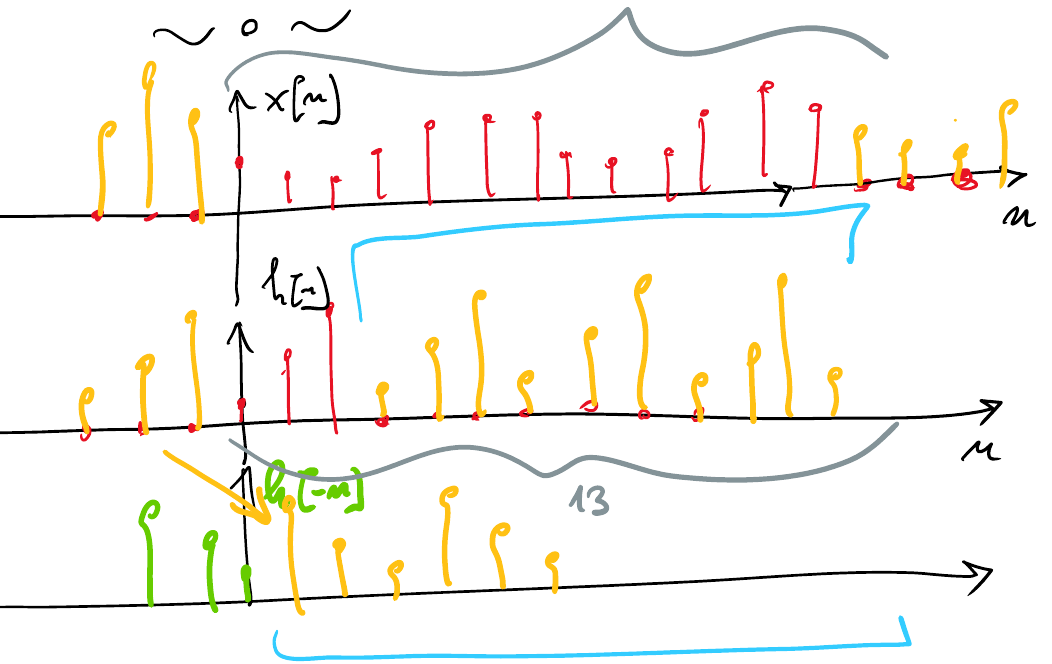
\includegraphics[scale=0.35]{immagini/lez25/convoluzioneDFT.jpg}
\end{figure}

possiamo quindi dare la proprieta' della convoluzione della DFT, se i campioni dei due segnali sono uguali:

\[
x_p[n] * h_p[n] \leftrightarrow  X_{[k]} H_{[k]} \mbox{ SE } M = N
\]

Ma come possiamo rendere $M = N$, i due segnali di lunghezza uguale?
Esiste una tecnica chiamata ZERO PADDING che consiste nel mettere tanti zeri nella sequenza piu' corta.
Dimostriamo che funziona:
\[\begin{split}
    x[n] \leftrightarrow X_{[k]} = \sum_{n=0}^{N-1} x[n] e^{-j \frac{2\pi}{N}kn} \\
    \Tilde{x}[n] = \{x[n]; 0 \mbox{ ... }0\} \leftrightarrow \Tilde{T}_{[k]} = \sum_{n=0}^{2N-1} \Tilde{x}[n] e^{-j \frac{2\pi}{2N}kn} \\
    = \sum_{n=0}^{N-1} x[n] e^{-j \frac{2\pi}{2N}kn} \\
    k = 2h\\
    \mbox{Quando k pari } = \sum_{n=0}^{N-1} x[n] e^{-j \frac{2\pi}{N}hn}
\end{split}\]

Allargando il segnale con tanti zeri abbiamo portato un aumento della visibilita' spettrale, che e' passata da $\frac{2\pi}{N}$ a $\frac{2\pi}{2N}$. Ovvero parlando in termini pratici ho piu' campioni con frequenze piu' vicine tra di loro (griglia di campionamento piu' fine).

Ma per i valori dispari cosa abbiamo ottenuti? Succede che la DFT viene campionata in punti che precedentemente non avevamo. Questa e' una cosa che molto spesso viene ricercata e nel calcolo numerico e' una tecnica spettrale.


\begin{figure}[ht!]
    \centering
    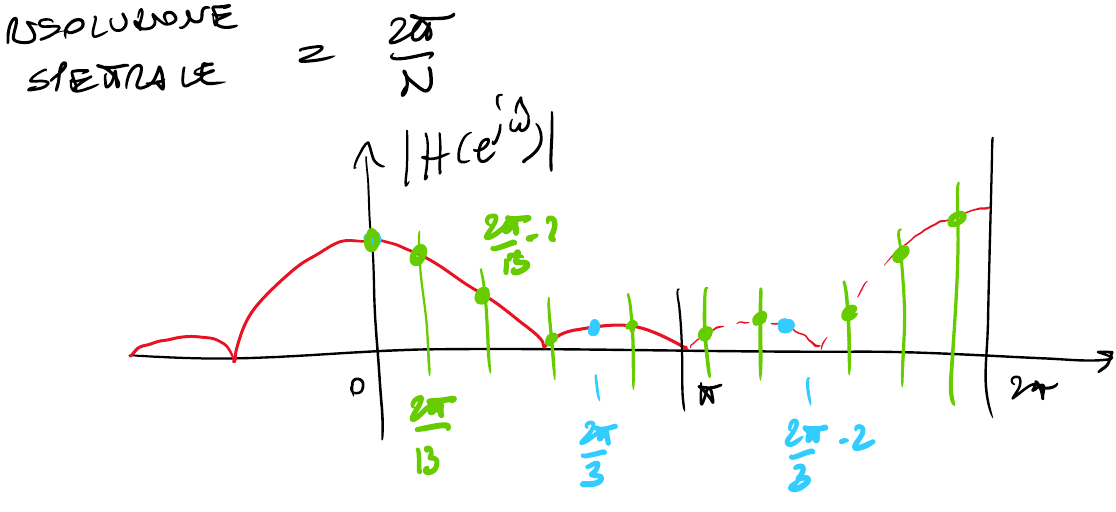
\includegraphics[scale=0.35]{immagini/lez25/aumentoRisoluzioneSpettrale.jpg}
\end{figure}

\section{Riassuno filtraggio LTI}

\begin{figure}[ht!]
    \centering
    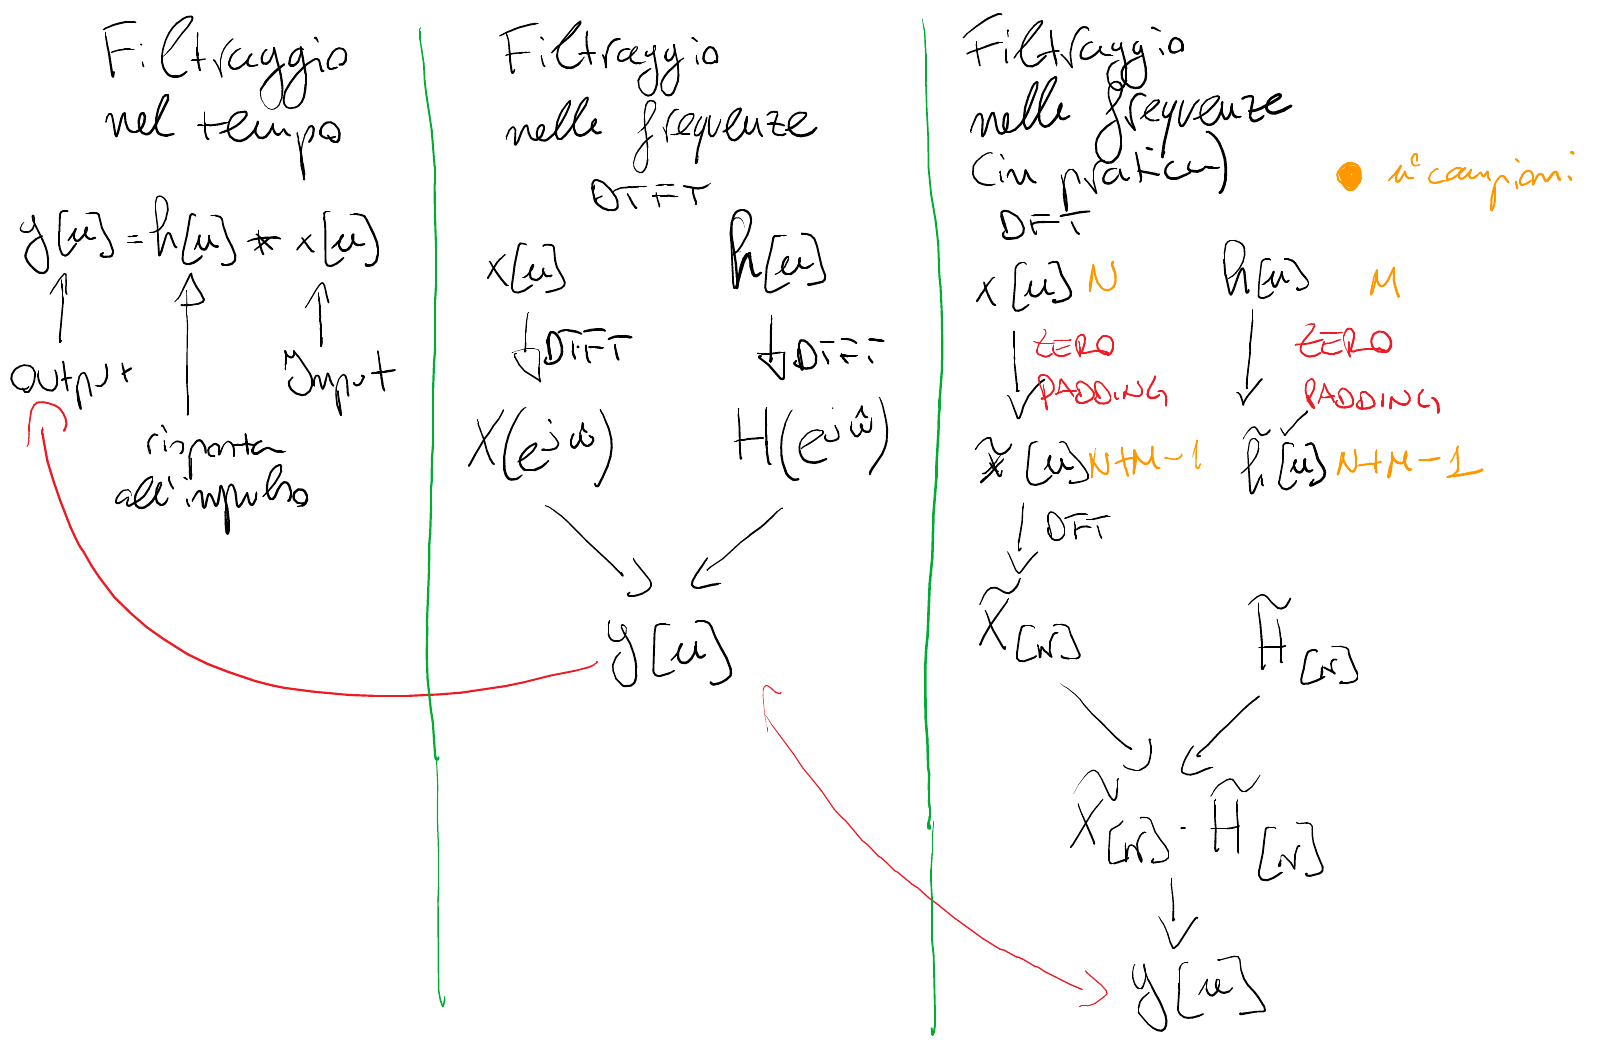
\includegraphics[scale=0.35]{immagini/lez25/filtraggio.jpg}
\end{figure}

Possiamo provare a calcolare il filtraggio utilizzando la DFT e lo zero padding.
Comunque notiamo che il problema delle repliche nelle convoluzione e' presente lo stesso ma abbiamo visto che aggiungendo degli zeri al segnale abbiamo allontanato le repliche spettrali dall'alias principale, quindi l'intuizione e' di aggiungere altri zeri in modo da poter fare una convoluzione "pulita". Ma di quanti zeri ho bisogno? N+M-1 campioni ad entrambi i segnali (non solo il piu' corto).

\begin{figure}[ht!]
    \centering
    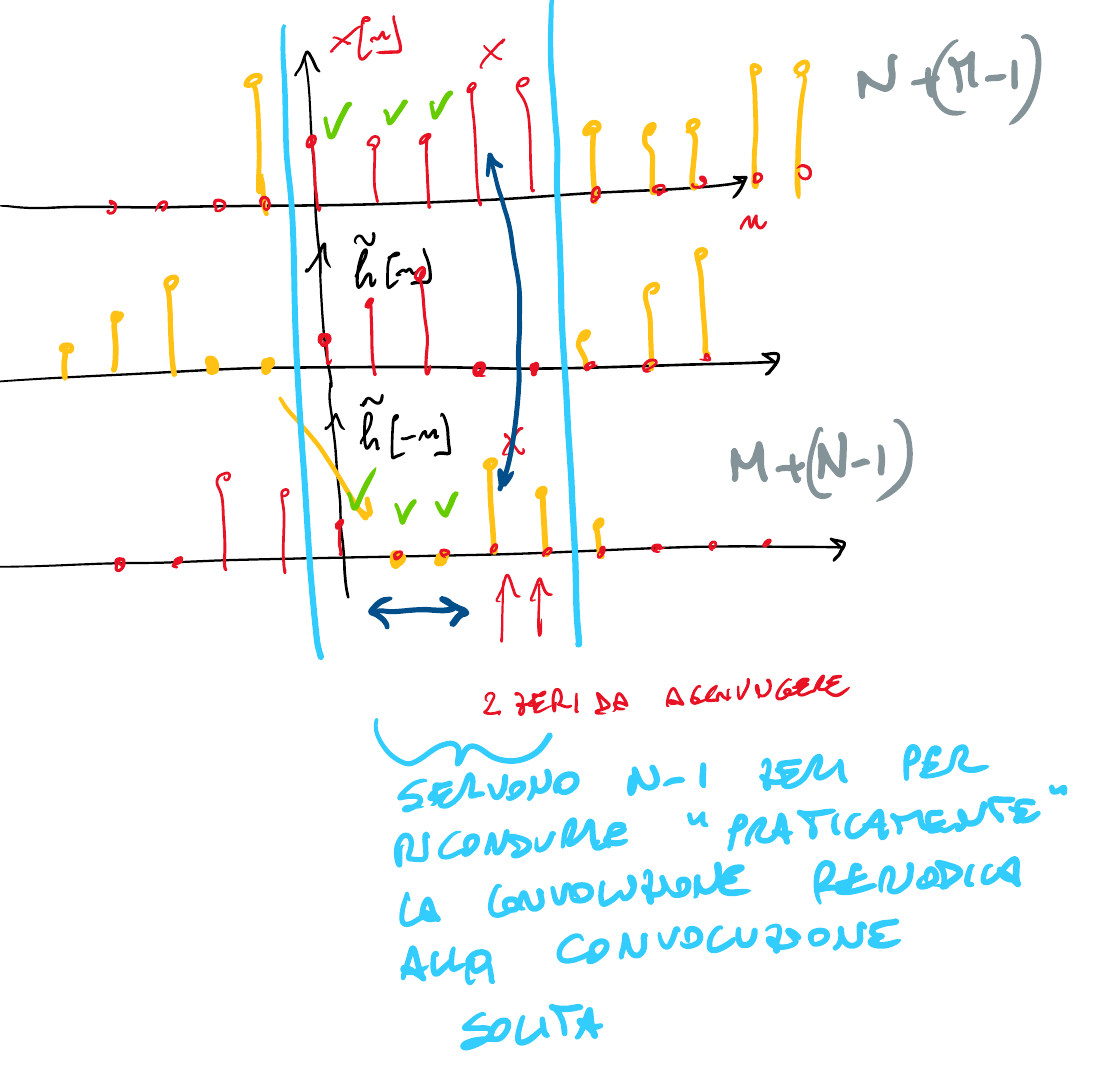
\includegraphics[scale=0.35]{immagini/lez25/convoluzioneZeroPadding.jpg}
\end{figure}

\section{Fast Fourier Trasnsform FFT}

Quello che abbiamo visto con il filtraggio tramite DFT e' computazionalmente molto svantaggioso (e perdente rispetto agli altre due approcci). Ma si sono accorti che la DFT si puo' calcolare semplicemente implementando un algoritmo, tanto semplicemente che a volte e' un'implementazione inclusi direttamente in hardware. 
L'algoritmo per calcolare semplicemente la DFT si chiama Fast Fourier Transform FFT. 
E' un algoritmo che fa parte della famiglia divide et impera, ovvero cerchiamo di dividere il problema in sotto problemi fino ad arrivare ad una "foglia" che e' facilmente risolvibile e successivamente tornare su tramite la ricorsione. Teoricamente e' un algoritmo ricorsivo, ma nella pratica non e' implementato in maniera ricorsiva, perche' e' un implementazione che costa meno.

Vediamo come funziona. Abbiamo una sequenza di campioni che e' lunga una potenza di due $N = 2^M$ (oggi non e' piu' obbligatorio che lo sia, ma e' il caso migliore), l'idea e' di prendere i numeri negli indici pari e metterli in un altro vettore e fare la stessa cosa con i numeri negli indici dispari, ripetere queste istruzioni finche' il vettore e' composto di due elementi. Una volta che ho tanti vettori composti da due elementi siamo arrivati al caso base. Ma perche' e' questo il caso base? Semplicemente perche' per calcolare la DFT di un vettore con due elementi devo fare 0 moltiplicazioni e di conseguenza e' molto poco oneroso computazionalmente.

\begin{figure}[ht!]
    \centering
    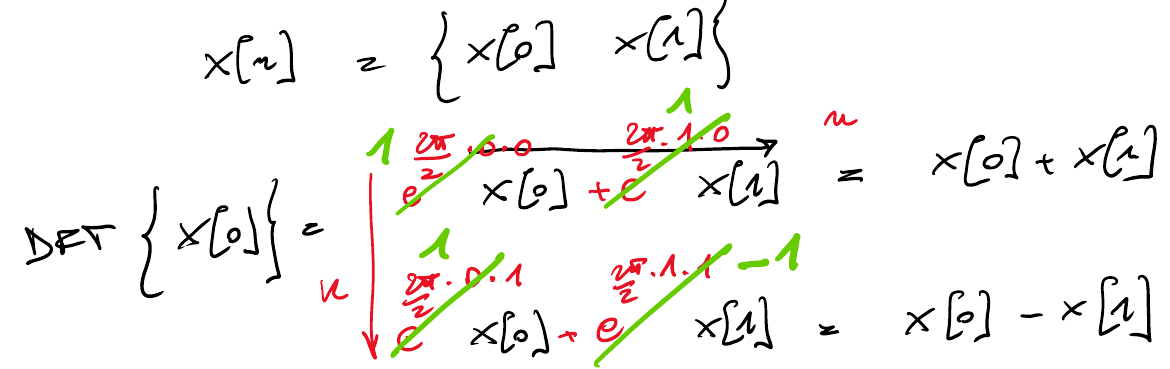
\includegraphics[scale=0.35]{immagini/lez25/DFT2Elementi.jpg}
\end{figure}

A questo punto, dopo aver capito qual'e' il caso base della ricorsione, dobbiamo tornare indietro e ricostruire i vari vettori partendo dal casi base.
Consideriamo una DFT generale di un segnale, ci siamo posti nella condizione in cui $N=2^M$, possiamo spaccare la sommatoria in due, in una consideriamo i numeri pari e nell'altra i numeri dispari:

\[\begin{split}
    X_{[k]} &= \sum_{n=0}^{N-1} x[n] e^{-j \frac{2\pi}{N}\cdot kn} \\
    &= \sum_{l=0}^{\frac{N}{2}-1} x[2l] e^{-j \frac{2\pi}{N}\cdot 2lk} + \sum_{l=0}^{\frac{N}{2}-1} x[2l+1] e^{-j \frac{2\pi}{N}\cdot (2l+1) k}\\
    \mbox{Riscriviamo } e^{-j \frac{2\pi}{N}\cdot (2l+1) k} &= e^{-j \frac{2\pi}{N}\cdot 2l k} e^{-j \frac{2\pi}{N}\cdot k} \\
    &\mbox{Portiamo furi l'esponenziale che non dipende da l} \\
    &= \sum_{l=0}^{\frac{N}{2}-1} x[2l] e^{-j \frac{2\pi}{N}\cdot 2lk} + (e^{-j \frac{2\pi}{N}k}) \sum_{l=0}^{\frac{N}{2}-1} x[2l+1] e^{-j \frac{2\pi}{N}\cdot lk} \\
\end{split}\]

Abbiamo quindi ottenuto una sommatoria dei valori pari piu' una sommatoria dei valori dispari moltiplicata per un fattore che ad ogni iterazione scala (0,1,2 ... N).

Guardiamo adesso una tabella che ci fa capire praticamente quanto e' piu' vantaggiosa la FFT in termini di moltiplicazioni rispetto alle DFT:

\begin{table}[ht!]
    \centering
    \begin{tabular}{c|c|c}
        N & Moltiplicazioni FFT & Moltiplicazioni DFT  \\
        \hline
        2 & 0 & 4 \\
        4 & $2 \cdot 0 + 4 = 4$ & 16 \\
        8 & $2 \cdot 4 + 8 = 16$ & 64 \\
        16 & $2 \cdot 16 + 16 = 44$ & 256 \\
        N & $N(\log_2 N-1)$ & $N^2$ \\
        1000 & $2,8 \cdot 10^4$ & $10^6$ \\
        $10^6$ & $5,8 \cdot 10^7$ & $10^12$ \\
    \end{tabular}
\end{table}

\subsection{Costo computazionale filtraggio nel tempo (convoluzoine) VS frequenza (DFT)}
\begin{figure}[ht!]
    \centering
    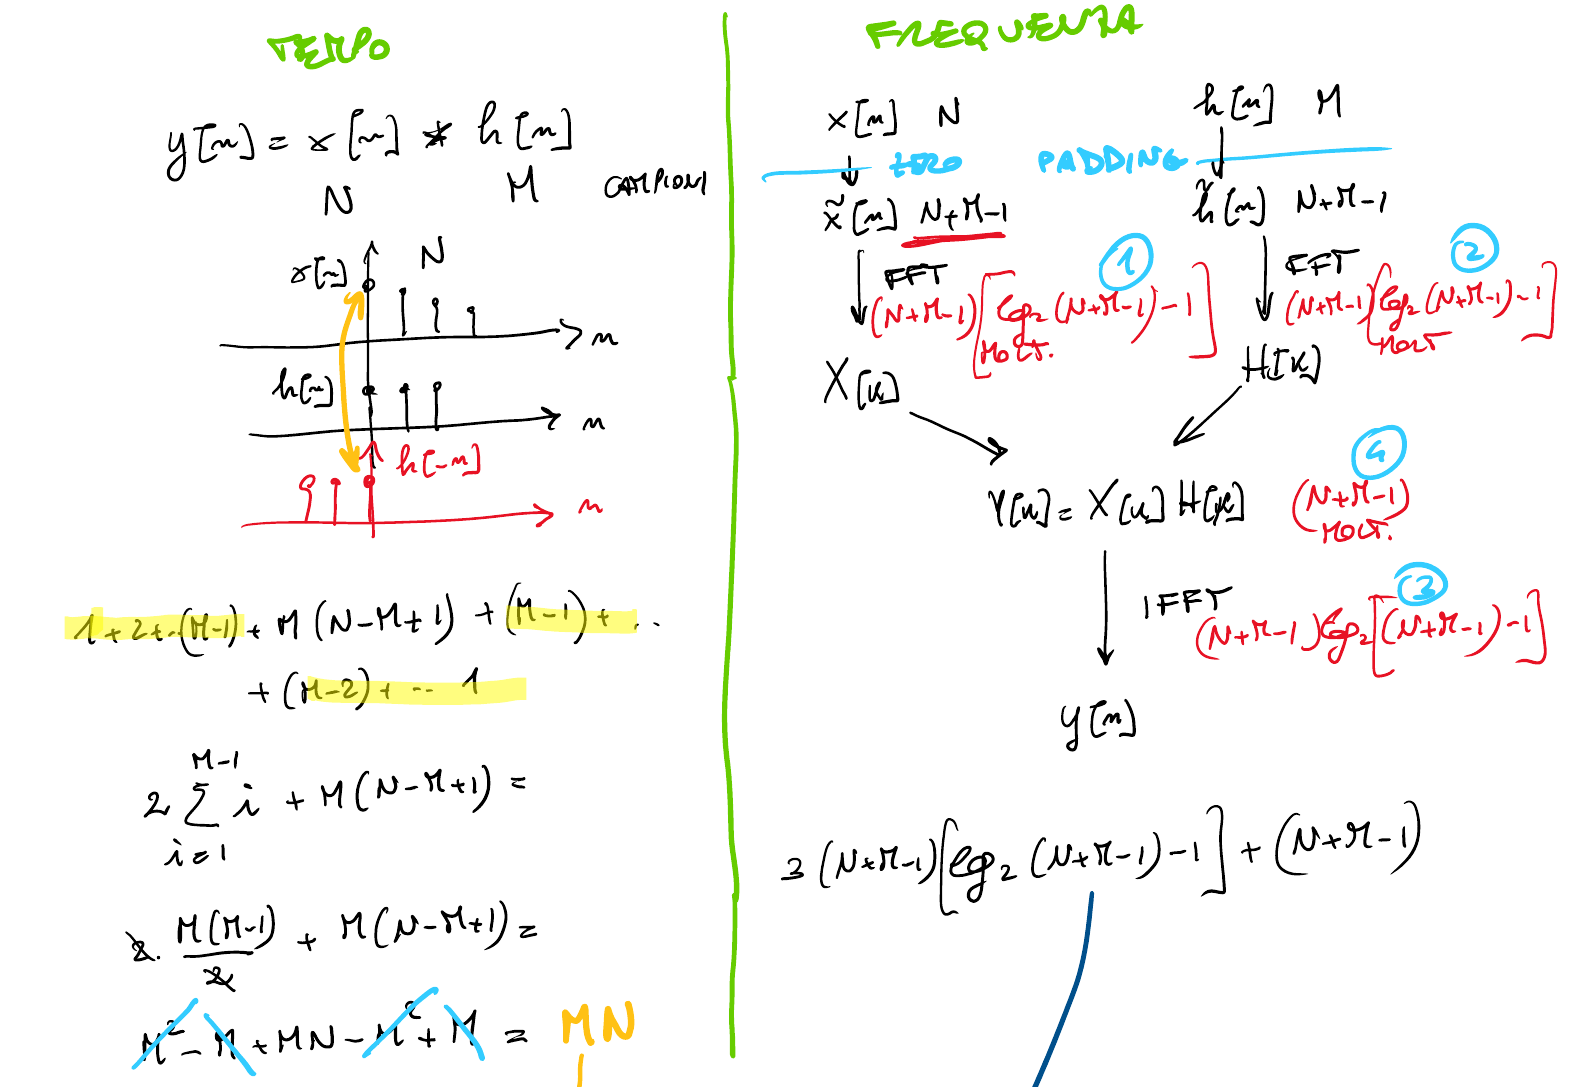
\includegraphics[scale=0.35]{immagini/lez26/convoluzioneTempoFrequenza.jpg}
\end{figure}

\begin{figure}[ht!]
    \centering
    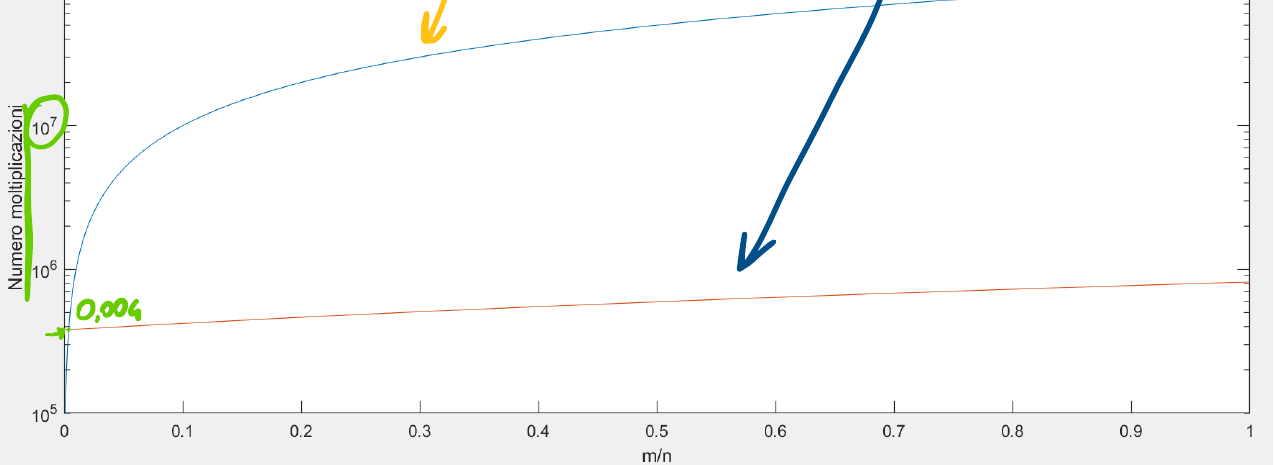
\includegraphics[scale=0.35]{immagini/lez26/graficoCostoFiltraggio.jpg}
\end{figure}

Da questo confronto tiriamo fuori una regola generale se M e' molto minore di N (ovvero il filtro e' corto) bisogna utilizzare il filtraggio nel tempo, viceversa se M e' simile ad N (ovvero il filtro e' lungo quanto il segnale) bisogna usare il filtraggio nelle frequenze, perche' in entrambi i casi sono computazionalmente meno onerosi.

\subsection{Base ortonormale}
Notiamo che a differenza di come avevamo fatto con la serie di Fourier e la DTFT, per la DFT non abbiamo visto una definizione che utilizza il prodotto scalare, questo perche' essendo la DFT un vettore numerabile, il prodotto scalare e' semplicemente il prodotto scalare del vettore per una base ortogonale.

Ma perche' ortogonale e non ortonormale, come invece era per serie di Fourier e DTFT?
Ricordiamo inizialmente che un vettore e' ortogonali quando prodotto scalare per una base e' 0. Dimostriamo quindi che facendo il prodotto vettoriale tra un elemento della DFT ed una base otteniamo 0:

\[\begin{split}
    <e^{j \frac{2\pi}{N}kn}; e^{j \frac{2\pi}{N}hn}> &= \sum_{n=0}^{N-1} e^{j \frac{2\pi}{N}kn} e^{j \frac{2\pi}{N}hn} \\
    &= \sum_{n=0}^{N-1} (e^{j \frac{2\pi}{N}})^{(k-h)n} = \frac{1 - e^{j \frac{2\pi}{N}kn}}{1 - e^{j\frac{2\pi}{N}}(k-h)}\\
    &= 
    \begin{cases}
    \frac{0}{N \neq 0} = 0 \text{ se } h \neq k \\
    N \text{ se } h=k\\
    \end{cases}
\end{split}\]

\subsection{Legge di conservazione (Parseval)}

\begin{equation}
    \sum_{n=0}^{N_1} |x[n]|^2 = \frac{1}{N} \sum_{k=0}^{N-1} |X_{[k]}|^2
\end{equation}

E' l'energia del segnale se il segnale ha supporto compatto, altrimenti se e' periodico e' l'energia nel periodo.

\chapter{Trasformata Z}
Grazie allo strumento di analisi (FFT o DFT) abbiamo capito meglio il filtraggio e ci siamo resi conto che e' algebricamente complicato. 
Dobbiamo quindi trovare degli strumenti piu' semplici per filtrare un segnale.
Per fare questo dobbiamo usare un nuovo operatore, che e' molto importante nell'analisi complessa, ma che a noi non interessa molto a livello teorico ma solamente a livello pratico, per semplificarci la vita.
L'idea che dobbiamo avere in mente e' che stiamo aggiungendo una dimensione ulteriore, in modo tale da vedere le cose piu' da lontano dato che risulteranno piu' facili.

L'operatore che introduciamo si chiama TRASFORMATA Z, ne diamo subito la definizione:

\begin{equation}
    \in \mathbf{C} \leftarrow X(z) = \sum_{n = -\infty}^{+\infty} x[n] z^{-n} \leftarrow \in \mathbf{Z}
\end{equation}

\begin{figure}[ht!]
    \centering
    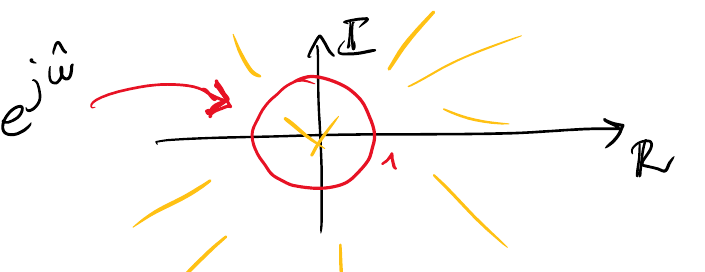
\includegraphics[scale=0.35]{immagini/lez26/trasformataZ.jpg}
\end{figure}

z e' quello che prima chiamavamo $e^{j \hat{\omega}}$, e grazie a questa generalizzazione notiamo che prima con la DTFT potevamo stare solamente sul cerchio unitario, in quanto $e^{j \hat{\omega}}$ valeva 1 in quei punti, mentre ora posso muovermi lungo tutto il piano (tranne dentro al cerchio).

\subsection{Esempio 1}

Consideriamo il seguente segnale e calcoliamone la trasformata Z:

\begin{figure}[ht!]
    \centering
    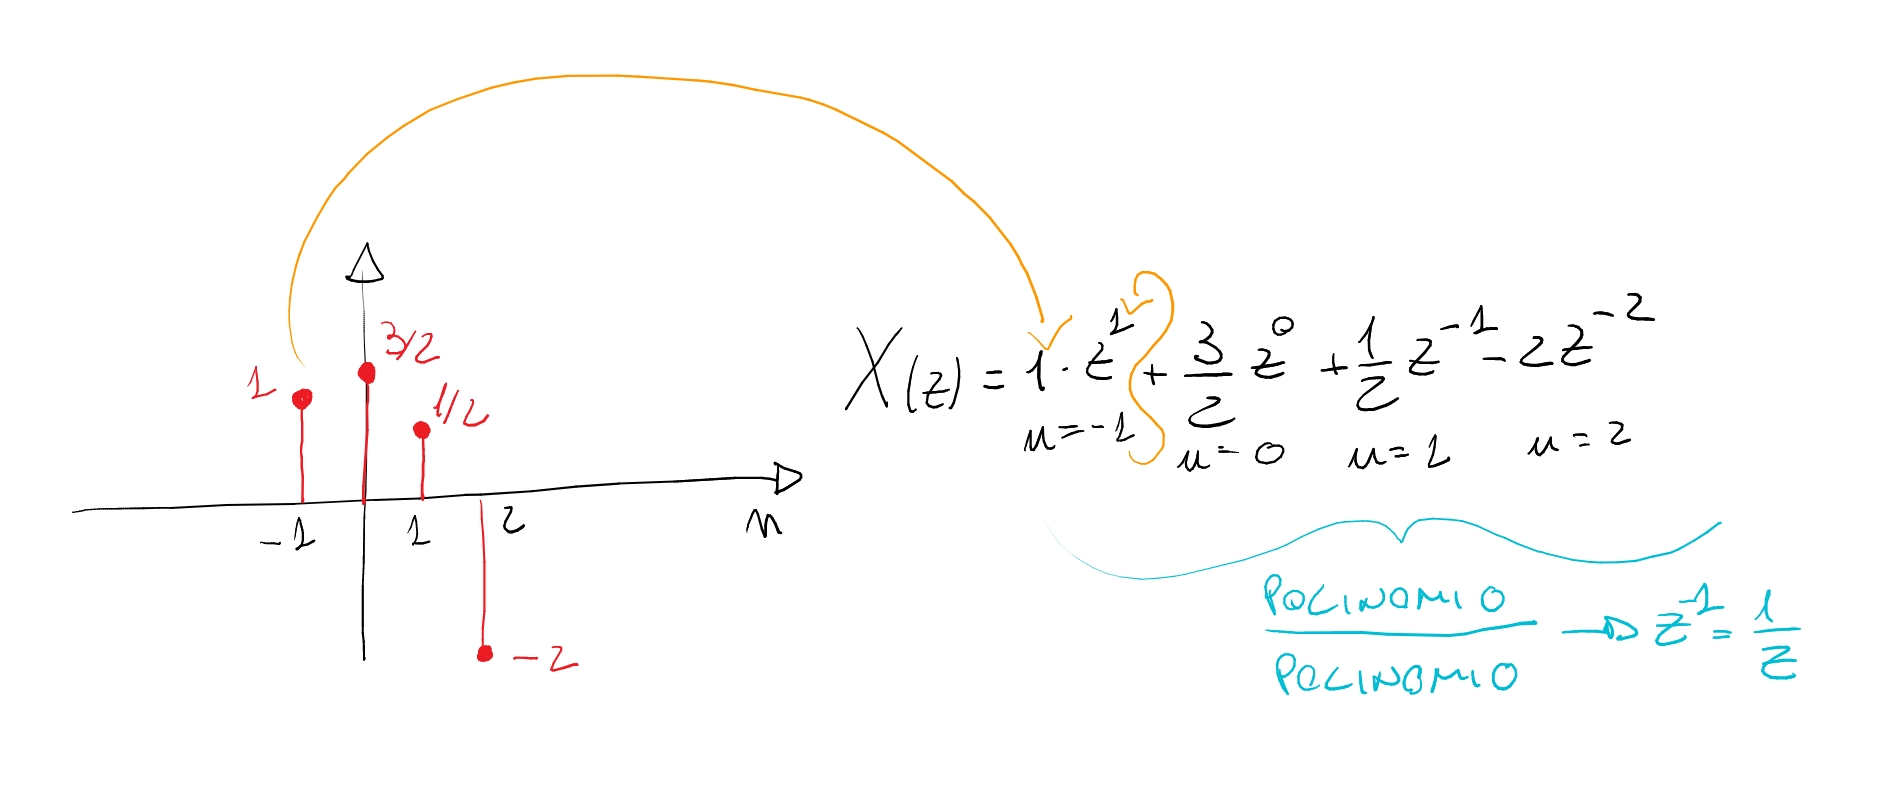
\includegraphics[scale=0.2]{immagini/lez26/es1TrasZ.jpg}
\end{figure}

Notiamo che abbiamo ottenuto tutti polinomi, diversamente da quanto succedeva con la DTFT dove ottenevamo una sommatoria di esponenziali complessi. Quindi possiamo dire che X(z) E' SEMPRE UN RAPPORTO DI DUE POLINOMI.

\subsection{Esempio 2}

Ora consideriamo il seguente segnale:

\[
x[n] = a^n u[n]
\]

Che ricordiamo esistere solo se $|a|<1$.

\begin{figure}[ht!]
    \centering
    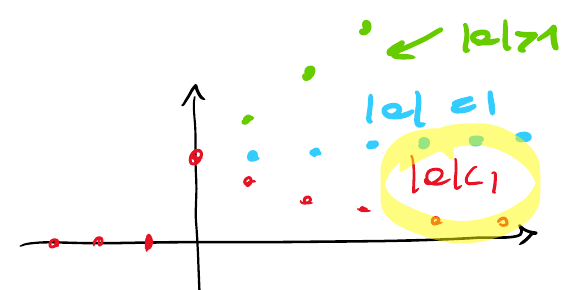
\includegraphics[scale=0.35]{immagini/lez26/esempio2.jpg}
\end{figure}

Troviamo la trasformata Z:

\[\begin{split}
    X(z) &= \sum_{n = -\infty}^{+\infty} a^n u[n] z^{-n} = \sum_{n=0}^{+\infty} (az^{-1})^n \\
    &\frac{1}{1 - az^{-1}} \mbox{ SE } |az^{-1}| < 1
\end{split}\]

$|az^{-1}| = \frac{|a|}{|z|} < 1 \leftarrow |z| > |a|$ e' molto importante e si chiama regione di convergenza ROC.

\begin{figure}[ht!]
    \centering
    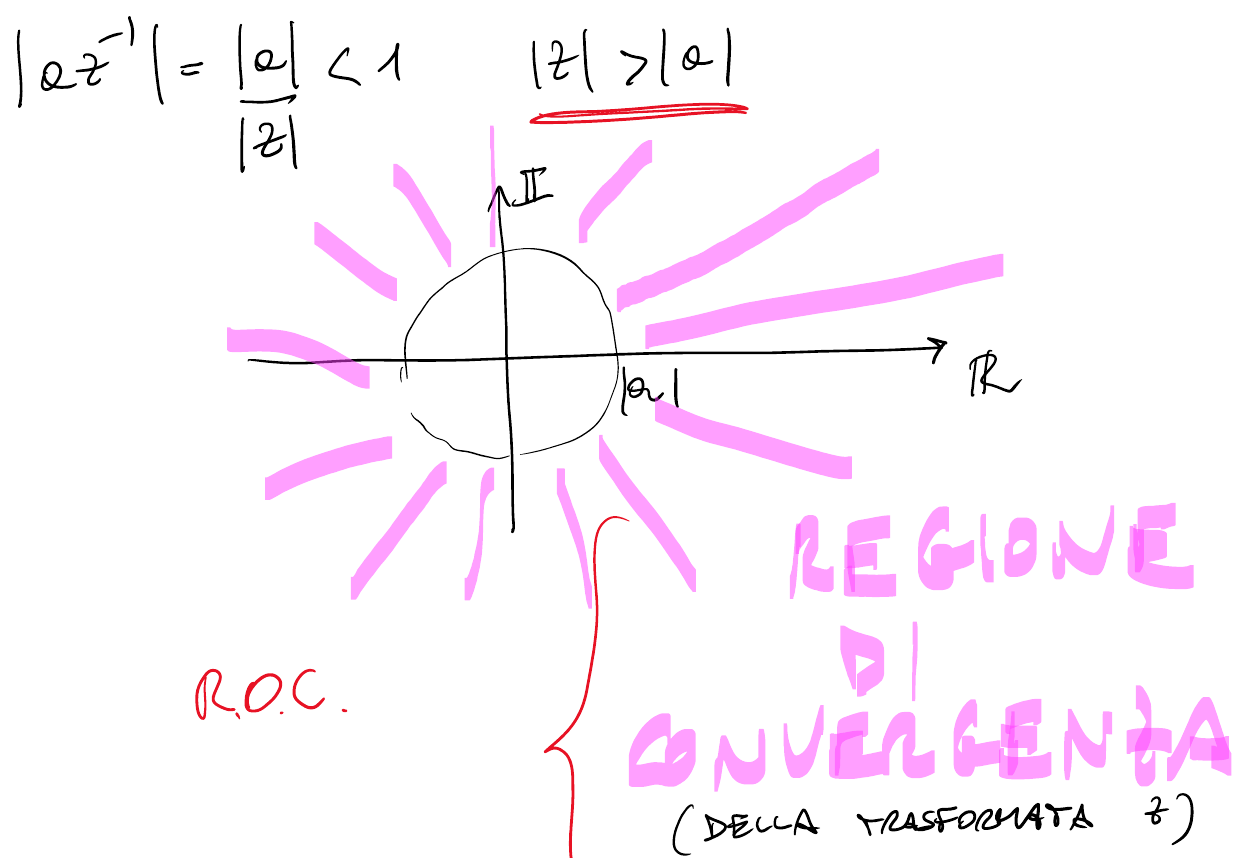
\includegraphics[scale=0.35]{immagini/lez26/regioneConvergenza.jpg}
\end{figure}

\newpage


\section{Trasformate note}
Vediamo due coppie di trasformate z (prese anche dagli esercizi che abbiamo fatto):

\[\begin{split}
    x[n] = a^n u[n] \leftrightarrow 
    \begin{cases}
    X(z) = \frac{1}{1 - a z^{-1}}\\
    R.O.C.: |z|>|a|\\
    \end{cases}\\
    x[n] = -a^n u[-n-1] \leftrightarrow 
    \begin{cases}
    X(z) = \frac{1}{1 - a z^{-1}}\\
    R.O.C.: |z|<|a|\\
    \end{cases}\\
\end{split}\]

Il primo e' chiamato gradino CAUSALE e notiamo che la sua ROC va verso infinito, mentre il secondo e' chiamato gradino ANTICAUSALE e la sua ROC va verso 0.

E' importante notare che, a differenza di quello che succedeva con la DTFT, la trasformata z non e' unica SE non la associamo alla sua ROC.
Possiamo quindi dire che $X(z) + ROC$ e' unica, quindi esiste un solo segnale di cui e' la trasformata z.

\section{Proprieta' della trasformata Z}
Vediamo ora tutte le proprieta' che ci serviranno della trasformata Z:

\subsection{Linearita'}

\[
    X(z) = \sum_{n = -\infty}^{+\infty} x[n] z^{-n}
\]

Notiamo che la trasformata z e' la composizione lineare di operatori lineari:
\begin{itemize}
    \item Somme
    \item Prodotti
    \item Costanti
\end{itemize}
Quindi e' anch'esso un operatore lineare.

\subsection{Ritardo temporale}
Questa e' una proprieta' molto importante per svolgere gli esercizi, vediamo cosa succede alla trasformata z quando ritardiamo il segnale di $n_0$ campioni:

\[\begin{split}
    x[n] &\leftrightarrow
    \begin{cases}
    X(z)\\
    R.O.C.\\
    \end{cases}\\
    x[n - n_0] &\leftrightarrow
    \begin{cases}
    X(z) \cdot z^{-n_0}\\
    R.O.C.
    \end{cases}
\end{split}\]

Vediamo che la trasformata e' moltiplicata per un fattore $z^{-n_0}$, dimostriamolo:

\[\begin{split}
    Z\{x[n-n_0]\} &= \sum_{n = -\infty}^{+\infty} x[n-n_0] z^{-n} \\
    \mbox{Cambio di variabile: } m &= n - n_0, n = m + n_0 \\
    &= \sum_{n = -\infty}^{+\infty} x[m] z^{-m -n_0} \\
    &=z^{-n_0} \sum_{m = -\infty}^{+\infty} x[m] z^{-m} = z^{-n_0} X(z)
\end{split}\]

\subsection{Convoluzione}
La convoluzione si trasforma in moltiplicazione:

\[
    x[n] * y[n] \leftrightarrow X(z) \cdot Y(z)
\]

\newpage

\subsection{ROC ha sempre simmetria radiale}
La trasformata z assume lo stesso valore per ogni $|z| = a$

\begin{figure}[ht!]
    \centering
    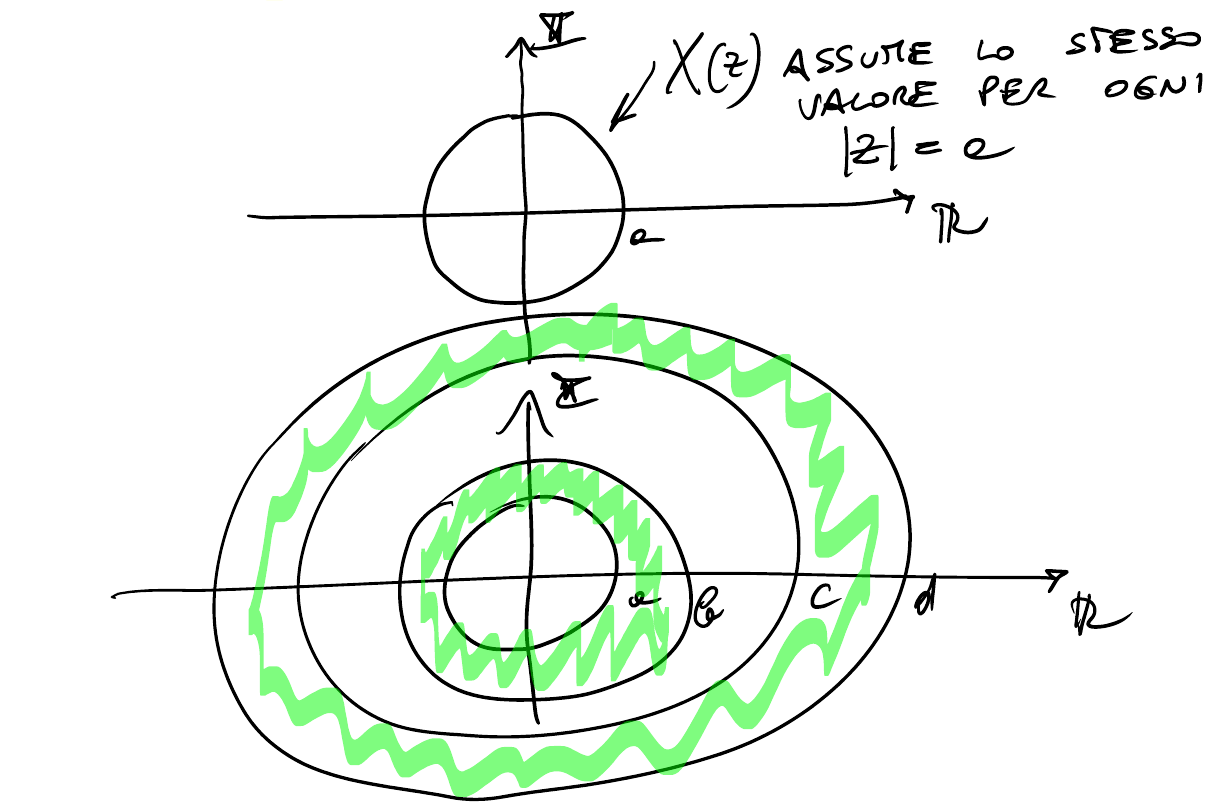
\includegraphics[scale=0.4]{immagini/lez27/ROCsimmetriaRadiale.jpg}
\end{figure}

Questo succede che la il modulo della trasformata z, che e' una sommatoria non deve divergere, ma notiamo che la trasformata dipende solo dal modulo, non dalla fase che invece puo' ruotare anche all'infinito ruotando intorno alla circonferenza, ed e' per questo che il $|X(z)|$ dipende solo dal modulo di z, che e' uguale su ogni circonferenza, con centro l'origine. Ne deriviamo quindi la simmetria radiale della ROC:

\[\begin{split}
    |X(z)| &= |\sum_{n = -\infty}^{+\infty} x[n] z^{-n}| \\
    &\le \sum_{n = -\infty}^{+\infty} |x[n] z^{-n}| = \sum_{n = -\infty}^{+\infty} |x[n]| |z^{-n}|
\end{split}\]
\newpage

\subsection{Nota a margine}
Negli schemi circuitali c'e' un segno particolare che e' il ritardo di un campione, che ha il simbolo del ritardo della trasformata z, non ha nulla a che vedere con la trasformata z, ma si rifa' alla sua proprieta' del ritardo temporale:

\begin{figure}[ht!]
    \centering
    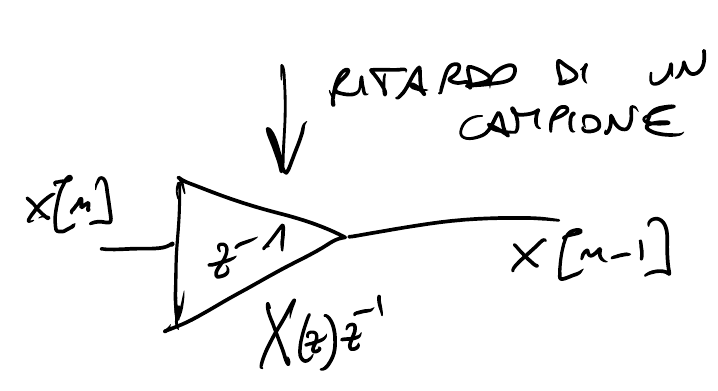
\includegraphics[scale=0.4]{immagini/lez27/notaMargine.jpg}
\end{figure}

\section{Funzione di trasferimento}

Partiamo ricordando qual'e' l'output di un sistema LTI:

\begin{figure}[ht!]
    \centering
    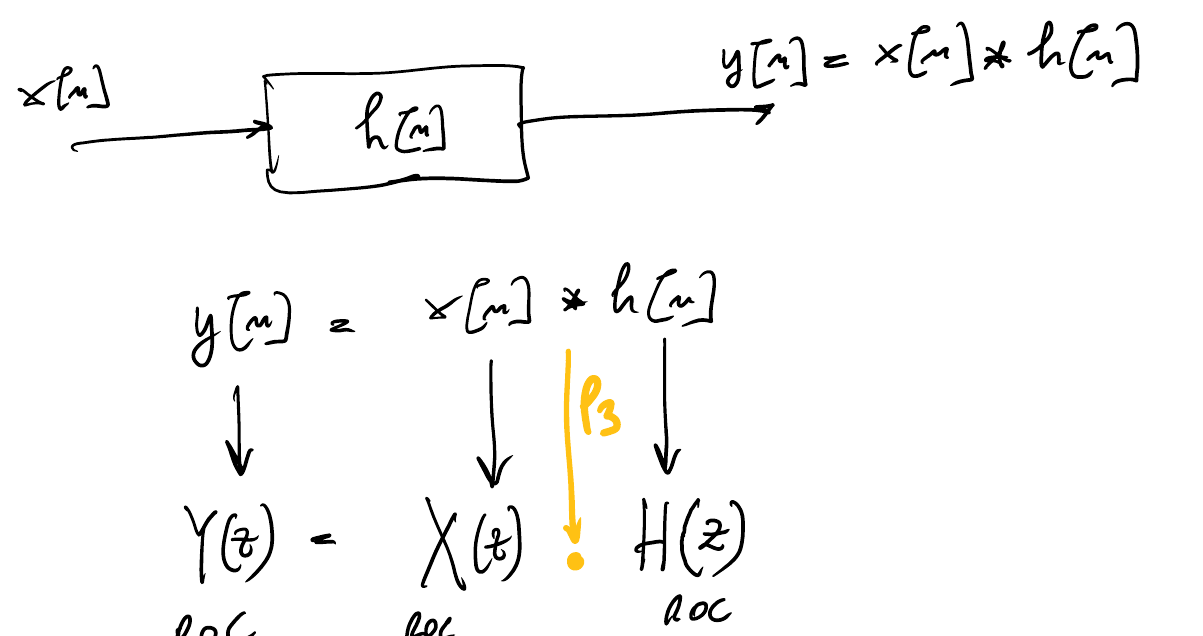
\includegraphics[scale=0.4]{immagini/lez27/funzioneTrasferimento.jpg}
\end{figure}

Vediamo che si facciamo la trasformata z di ogni elemento nell'equazione dell'uscita di un sistema LTI, applicando inoltre la proprieta' della trasformata che trasforma la convoluzione in moltiplicazione e successivamente raccogliamo la trasformata z della risposta all'impulso otteniamo la FUNZIONE DI TRASFERIMENTO:

\[
    Z\{h[n]\} = H(z) = \frac{Y(z)}{X(z)}
\]

E' chiamata funzione di trasferimento perche' trasferisce l'ingresso sull'uscita.

\subsection{$H(z)$ per un sistema LTI qualunque}

Vediamo ora come trovare la funzione di trasferimento partendo dall'equazione alle differenze di un sistema LTI qualunque, lo facciamo applicando le proprieta' che abbiamo appena visto:

\[\begin{split}
    &y[n] = \sum_{h = -N_1, h \neq 0}^{N_2} ah y[n-h] + \sum_{k = -M_1}^{M_2} bk x[n-k]\\
    &\mbox{Troviamo la trasformata z di ogni fattore ed applichiamo la proprieta' di linearita'}\\
    &Y(z) = \sum_{h = -N_1, h \neq 0}^{N_2} ah Z\{y[n-h]\} + \sum_{k = -M_1}^{M_2} bk Z\{x[n-k]\}\\
    &\mbox{Applichiamo la proprieta' del ritardo temporale per i segnali y e x:}\\
    &Y(z) = \sum_{h = -N_1, h \neq 0}^{N_2} ah Y(z) z^{-h} + \sum_{k = -M_1}^{M_2} bk X(z) z^{-k}\\
    &\mbox{Portiamo a sinistra i fattori che dipendono dalla trasformata Y:}\\
    &Y(z) - Y(z) \sum_{h = -N_1, h \neq 0}^{N_2} ah z^{-h} = X(z) \sum_{k = -M_1}^{M_2} bk  z^{-k}\\
    &\frac{Y(z)}{X(z)} = \frac{\sum_{k = -M_1}^{M_2} bk  z^{-k}}{\sum_{h = -N_1, h \neq 0}^{N_2} ah z^{-h}} = H(z)
\end{split}\]

E' importante notare che la funzione di trasferimento e' sempre una funzione razionale fratta (frazione tra due polinomi).

\section{Ripasso dell'algebra polinomiale}
Ricordiamo che un qualsiasi polinomio:
\[
    a_N z^N + a_{N-1}z^{N-1} +...+ a_1 z^1 + a_0 = 0
\]

Lo possiamo caratterizzare in due modi, o con i coefficienti:
\[
    a_0, a_1, a_2, ..., a_n
\]
Abbiamo quindi N+1 coefficienti.

Oppure fattorizzandolo (lo esprimiamo come prodotto di due o piu' fattori polinomiali di grado inferiore):
\[
    a_N(z - z_1)(z - z_2)...(z-z_N)
\]
Abbiamo quindi N radici appartenenti a C + un coefficiente ($a_n$).

Ricordiamo anche il teorema fondamentale dell'algebra che dice che per ogni polinomio di grado N ammette N soluzioni di C. Per ogni polinomio di grado N a coefficienti reali ammette N soluzioni reali o complesse coniugate.

\section{Zeri e Poli}
Riscriviamo la funzione di trasferimento di un generico sistema LTI fattorizzando i polinomi al numeratore ed al denominatore, notando che al numeratore abbiamo un polinomio di grado M, dove $M = M_1 + M_2$, mentre al denominatore abbiamo un polinomio di grado N, dove $N = N_1 + N_2$:

\[\begin{split}
    H(z) &= \frac{\sum_{k = -M_1}^{M_2} bk  z^{-k}}{\sum_{h = -N_1, h \neq 0}^{N_2} ah z^{-h}} \\
    &= \frac{b_M(z - z_1)(z-z_2) ... (z - z_M)}{a_N(z - p_1)(z-p_2) ... (z - p_N)}
\end{split}\]

e chiamiamo le radici $z_i$ del numeratore N(z) "ZERI", mentre chiamiamo le $p_i$ radici del denominatore D(z) "POLI".

\subsection{Esempio di zero}
Vediamo come si rappresenta una ZERO generico della funzione di trasferimento sul piano.
Consideriamo una generica trasformata z:

\[
    \epsilon(z) = |z - z_i|, z_i \in \mathbf{C}
\]

Possiamo inizialmente visualizzare il grafico di questa funzione immaginando che z e $z_i$ siano due vettori su un piano cartesiano, il modulo della differenza e' la distanza tra i due vertici del vettore, quindi possiamo dire che se z e' simile a $z_i$ (quasi coincidono) la funzione epsilon (ovvero il modulo della differenza) tendera' a 0, mentre se il modulo di z e' molto maggiore rispetto al modulo di $z_i$ possiamo dire che la funzione epsilon crescera' all'infinito.

\begin{figure}[ht!]
    \centering
    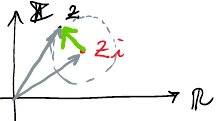
\includegraphics{immagini/lez28/zeroBidimensionale.jpg}
\end{figure}

Facciamo ora un ulteriore passo ricordandoci che la trasformata z gode della proprieta' di simmetria radiale, quindi in realta' la funzione epsilon sara' caratterizzata da tutti i punti sulla circonferenza centrata in $z_i$ con raggio la distanza tra $z_i$ e z.
Ora se aumentiamo di una dimensione il piano complesso, come avevamo detto avremmo fatto quando abbiamo iniziato a parlare della trasformata z, possiamo vedere che lo ZERO della funzione di trasferimento e' un cono centrato in $z_i$ (lo zero) che si allarga salendo lungo l'asse z (man mano che z aumenta).

\begin{figure}[ht!]
    \centering
    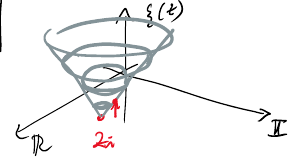
\includegraphics{immagini/lez28/zeroTridimensionale.jpg}
\end{figure}

\section{Esempi}
Vediamo adesso una serie di esempi, ma prima diamo la definizione di PRODUTTORIA, che ci serve per poter riscrivere la funzione di trasferimento. Produttoria:

\[
    \prod_{i = 1}^{N} x_i = x_1 \cdot x_2 \cdot x_3 \cdot x_4 ... \cdot x_N
\]


\[
    |H(Z)| = |\frac{b_M \prod_{i = 1}^M (z - z_i)}{a_N \prod_{j = 1}^N (p - p_j)}| = \frac{|b_M| \prod_{i = 1}^M |z - z_i|}{|a_N| \prod_{j = 1}^N |p - p_j|}
\]

Da questa definizione possiamo vedere delle caratteristiche degli ZERI, dato che il denominatore sara' piccolo quando siamo vicini ad uno zero, gli zeri tendono a far diventare piccola la funzione di trasferimento, graficamente possiamo immaginarlo come se schiacciassimo la funzione sul piano orizzontale.
Mentre per quanto riguarda i POLI, notiamo che NON possono essere nella regione di convergenza, perche' il denominatore della funzione di convergenza andrebbe a 0, quindi tutto tenderebbe ad infinito, questa cosa graficamente possiamo immaginarla come se i poli alzassero verso infinito la funzione, come un paletto che alza la tenda.

\subsection{Esempio 1}

Cominciamo da un esempio semplice, consideriamo:

\[
    H(z) = 1
\]

\newpage

Vediamo subito il grafico di questa funzione di derivazione:

\begin{figure}[ht!]
    \centering
    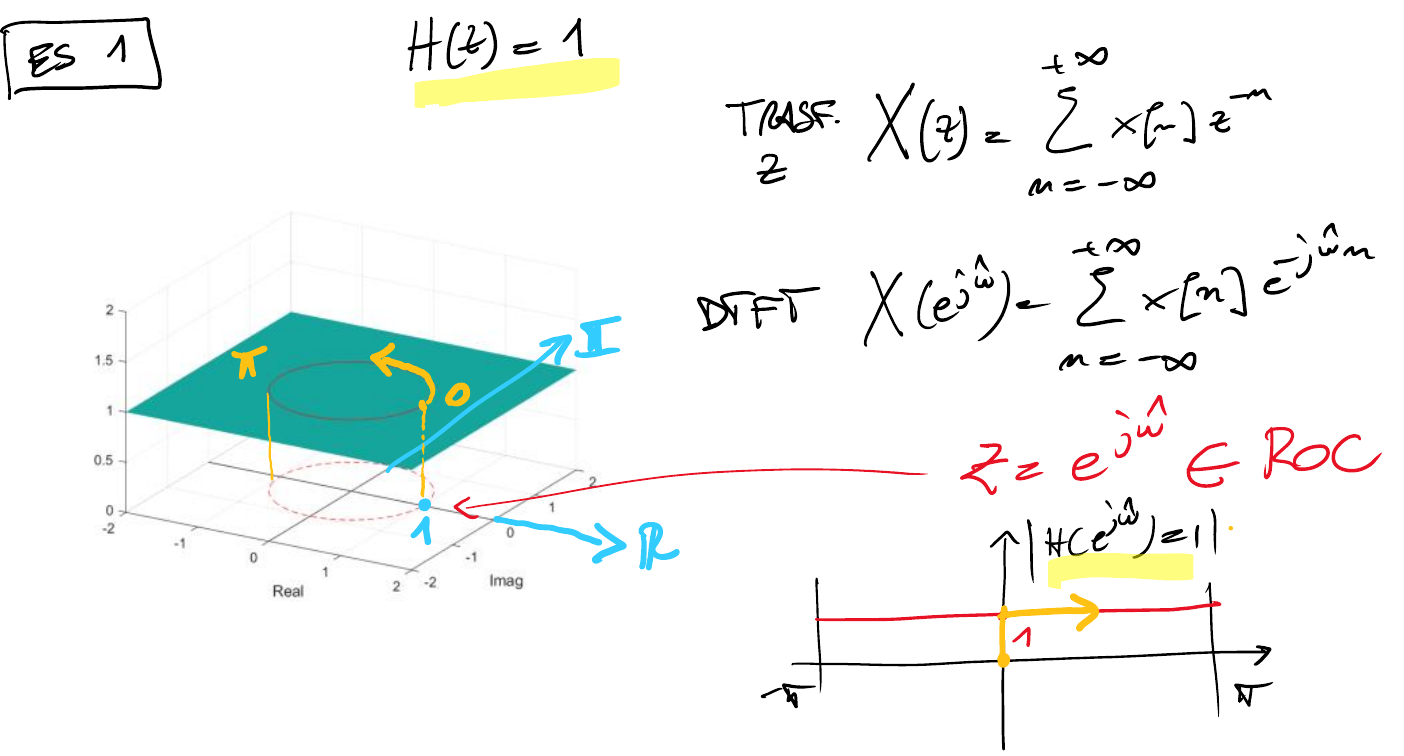
\includegraphics[scale=0.4]{immagini/lez28/es1.jpg}
\end{figure}

Vediamo che la funzione di trasferimento e' il piano verde, che e' un piano infinito che sta sopra al piano complesso, e' cosi' perche' ad ogni valore questa funzione associa 1.

Il cerchio invece e' la proiezione del cerchio unitario (la DTFT), quindi e' come se avessi trovato la risposta in frequenza del sistema che e' 1, e poi partendo dal punto 1 sul piano complesso, che corrisponde alla frequenza 0 sul grafico del modulo mi spostassi sul cerchio unitario. Facendo questa cosa posso riportare il movimento sul grafico del modulo dela risposta in frequenza.
Notiamo che lo possiamo fare perche' il cerchio unitario appartiene alla ROC della trasformata z.

\subsection{Esempio 2}
Ora vediamo una funzione di trasferimento piu' complessa:

\[
    H(z) = z - \frac{1}{2}
\]

Che notiamo essere nella forma $\varepsilon(z) = |z - z_i|$ e sappiamo gia' che il grafico di questa funzione di trasferimento e' un cono puntato in $z_i$, in questo caso in $\frac{1}{2}$, quindi possiamo dire che $\frac{1}{2}$ e' uno ZERO della funzione di trasferimento.

Ora dato che il cerchio unitario appartiene alla ROC, possiamo sostituire $z = e^{j \hat{\omega}}$ per trovare la risposta in frequenza:

\[
    H(e^{j\hat{\omega}}) = e^{j \hat{\omega}} - \frac{1}{2}
\]

Ora per disegnare il grafico del modulo della risposta in frequenza possiamo farlo in modo spannometrico guardando la proiezione del cerchio unitario sulla trasformata z. Ci poniamo inizialmente nel punto 1 sulla proiezione del cerchio unitario, che ricordiamo coincidere alla frequenza 0 nel grafico del modulo della risposta all'impulso, notiamo subito che e' il punto con altezza minore rispetto al piano complesso, non sappiamo esattamente quant'e', ma possiamo approssimarlo. Successivamente cominciamo a muoverci sul cerchio di raggio unitario fino ad arrivare al punto -1, che corrisponde alla frequenza $\pi$, notiamo che l'altezza dei punti che stiamo percorrendo rispetto al piano complesso aumenta fino al punto -1, e riportiamo questa informazione sul grafico del modulo.
Per disegnare il modulo da 0 a $-\pi$ semplicemente ribaltiamo lungo l'asse y la parte che abbiamo trovato tra 0 e $+\pi$.


\begin{figure}[ht!]
    \centering
    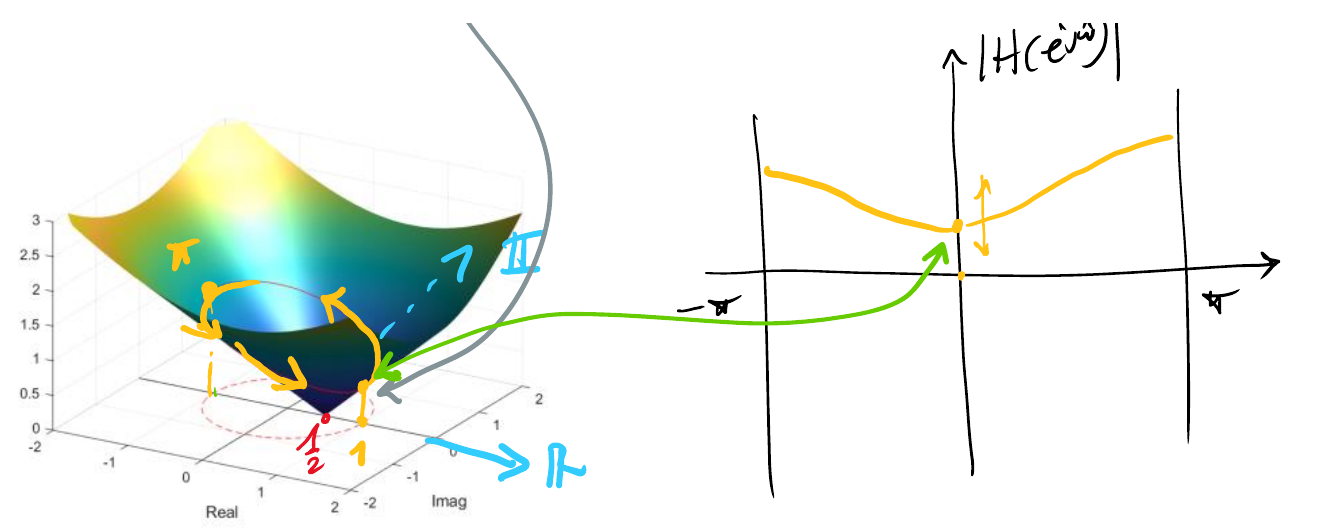
\includegraphics[scale=0.4]{immagini/lez28/es2.jpg}
\end{figure}

\subsection{Esempio 3}

Ora consideriamo:

\[
    H(z) = \frac{1}{z - \frac{1}{3}}
\]

Notiamo subito che il punto $\frac{1}{3}$ non appartiene alla ROC, perche' porterebbe il denominatore a 0, quindi e' un POLO, sappiamo quindi che il cerchio centrato nell'origine con raggio $\frac{1}{3}$ non appartiene alla ROC, questo potrebbe essere un problema perche' dobbiamo capire se il cerchio unitario appartiene alla ROC, in questo caso non abbiamo problemi perche' la funzione di trasferimento appartiene ad un gradino causale, sappiamo quindi che la ROC esiste per valori di z maggiori di a, quindi si estende da $\frac{1}{3}$ a $+\infty$.
Comunque possiamo sostituire $z = e^{j \hat{\omega}}$ in quanto il cerchio di raggio unitario appartiene alla ROC:

\[
    H(e^{j\hat{\omega}}) = \frac{1}{e^{j\hat{\omega}} - \frac{1}{3}}
\]

Per costruire il grafico del modulo della risposta in frequenza faccio come prima, mi porto nel punto 1 (che corrisponde alla frequenza 0) e mi muovo lungo la proiezione del cerchio unitario.

La cosa interessante di questo esempio e' vedere cosa succede quando e' presente un POLO, come abbiamo detto in precedenza il polo porta verso infinito la funzione. Per indicare la presenza di POLI e ZERI possiamo costruire un grafico POLI-ZERI, in cui indico con una X la presenza di un polo e con uno 0 la presenza di uno ZERO.

\begin{figure}[ht!]
    \centering
    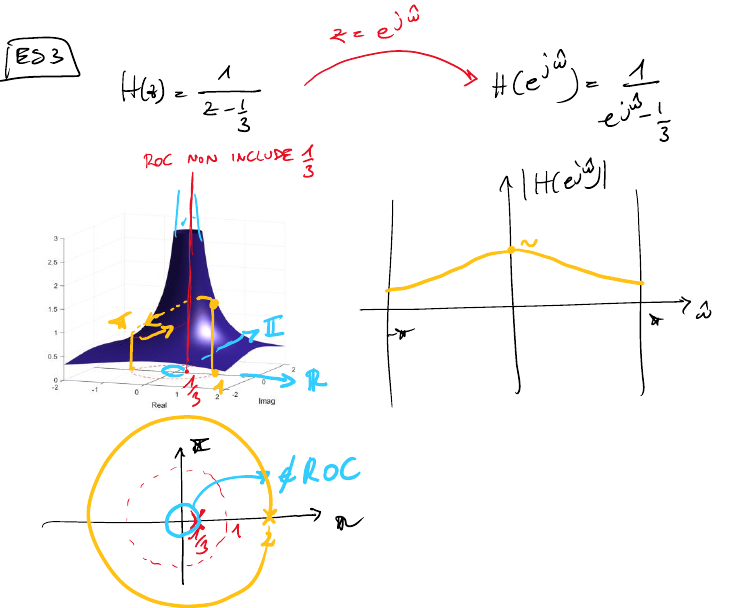
\includegraphics[scale=0.7]{immagini/lez28/es3.jpg}
\end{figure}

\newpage
\section{Dalla $H(z)$ all'equazione alle differenze}

Non abbiamo ancora visto qual'e' l'equazione alle differenze che genera la $H(z)$. Dobbiamo usare la trasformata z inversa: $z^{-1}$, ma non vedremo nessuna formula, useremo le coppie di trasformate z note.

Vediamolo per ogni esempio che abbiamo visto.

Esempio 1:

\[\begin{split}
    \frac{Y(z)}{X(z)} &= H(z) = 1\\
    Y(z) &= X(z)\\
    y[n] &= x[n]
\end{split}\]

Esempio 2:
\[\begin{split}
    \frac{Y(z)}{X(z)} &= H(z) = z - \frac{1}{2}\\
    Y(z) &= X(z) z^{-(-1)} - \frac{1}{2}X(z)\\
    y[n] &= x[n+1] -\frac{1}{2}x[n]
\end{split}\]

Abbiamo trovato un equazione FIR anticausale

Esempio 3:

\[\begin{split}
    \frac{Y(z)}{X(z)} &= H(z) = \frac{1}{z - \frac{1}{3}}\\
    Y(z) z - Y(z)\frac{1}{3} &= X(z)\\
    y[n+1] - \frac{1}{3}y[n] &= x[n]\\
    y[n] &= 3y[n+1] - 3x[n]
\end{split}\]

Abbiamo trovato un equazione IIR anticausale.

\section{Da $H(z)$ alla risposta all'impulso}
Se faccio la trasformata z inversa direttamente della funzione di trasferimento, trovo la risposta all'impulso. Lo facciamo sempre guardando le trasformate note.

Vediamo applicato a tutti gli esempi che abbiamo visto.

Esempio 1:

\[\begin{split}
    H(z) &= 1\\
    h[n] &= \delta[n]
\end{split}\]

Esempio 2:

\[\begin{split}
    H(z) &= z - \frac{1}{2} \\
    h[n] &= \delta[n + 1] - \frac{1}{2} \delta[n]
\end{split}\]

Esempio 3:

\[\begin{split}
    H(z) &= \frac{1}{z-\frac{1}{3}} = \frac{z^{-1}}{1 - \frac{1}{3} z^{-1}} \\
    &= \frac{1}{1 - \frac{1}{3} z^{-1}} \cdot z^{-1}
\end{split}\]

Qui pero' abbiamo un problema, perche' non sappiamo se e' un sistema causale o anticausale, ed il comportamento del gradino cambia in base al tipo di sistema, quindi se ROC: $|z| > |\frac{1}{3}$|, allora $h[n] = (\frac{1}{3})^{n-1} u[n-1]$.
Invece se ROC: $|z| < |\frac{1}{3}|$, allora $h[n] = -(\frac{1}{3})^{n-1} u[-(n-1)]$.

\newpage

\section{Esempio 4}
Partiamo adesso da un filtro causale FIR:

\[
    y[n] = x[n] - \sqrt{2} x[n-1] + x[n-2]
\]  

Da cui voglio ricavare il grafico del modulo della risposta in frequenza.
Per farlo ho a disposizione due procedure, una e' quella che usavamo fino ad adesso, ovvero troviamo la risposta all'impulso, da cui ricaviamo tramite la formula la risposta in frequenza, poi ci riconduciamo alla forma con il coseno e disegniamo il modulo del coseno.
Facciamolo:

\[\begin{split}
    h[n] &= \delta[n] - \sqrt{2} \delta[n-1] + \delta[n-2]\\
    H(e^{j\hat{\omega}}) &= 1 - \sqrt{2} e^{-j \hat{\omega}} + e^{-j 2 \hat{\omega}} \\
    &= 2e^{-j\hat{\omega}} \{\frac{e}{2}^{j\hat{\omega}} - \frac{\sqrt{2}}{2} + \frac{e}{2}^{-j\hat{\omega}}\} \\
    &= 2(\cos\hat{\omega} - \frac{\sqrt{2}}{2}) e^{-j\hat{\omega}}
\end{split}\]

\begin{figure}[ht!]
    \centering
    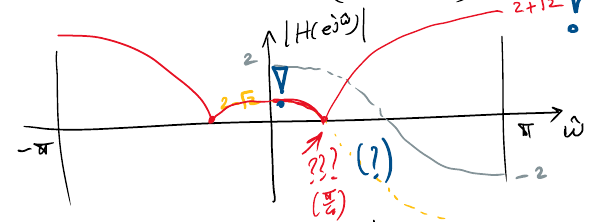
\includegraphics[scale=0.7]{immagini/lez28/es4.jpg}
\end{figure}

Utilizziamo adesso una seconda procedura trovando la funzione di trasferimento del sistema, successivamente trovare i zeri ed i poli della funzione, disegnare il grafico poli-zeri e da quello trovare il grafico approssimativo del modulo della risposta in frequenza.
Facciamolo:

\[\begin{split}
    &y[n] = x[n] - \sqrt{2} x[n-1] + x[n-2]\\
    &\mbox{Usiamo subito la proprieta' di linearita'}\\
    &Y(z) = X(z) - \sqrt{2} Z\{x[n-1]\} + Z\{x[n-2]\} \\
    &\mbox{Usiamo la proprieta' del ritardo}\\
    &Y(z) = X(z) - \sqrt{2} X(z) z^{-1} + X(z) z^{-2}\\
    &\frac{Y(z)}{X(z)} = 1 - \sqrt{2} z^{-1} + z^{-1} = \frac{z^2 - \sqrt{2}z + 1}{z^2}
\end{split}\]

Dobbiamo trovare gli ZERI:

\[\begin{split}
    &z^2 - \sqrt{2}z + 1 = 0 \\
    &Z_{1,2} = \frac{\sqrt{2} \pm \sqrt{2-4}}{2} = \frac{\sqrt{2} \pm i \sqrt{2}}{2} = \sqrt{\frac{2}{4} + \frac{2}{4}} e^{\pm i \frac{\pi}{4}}
\end{split}\]

ed i POLI:

\[
    p_1 = p_2 = 0
\]

\begin{figure}[ht!]
    \centering
    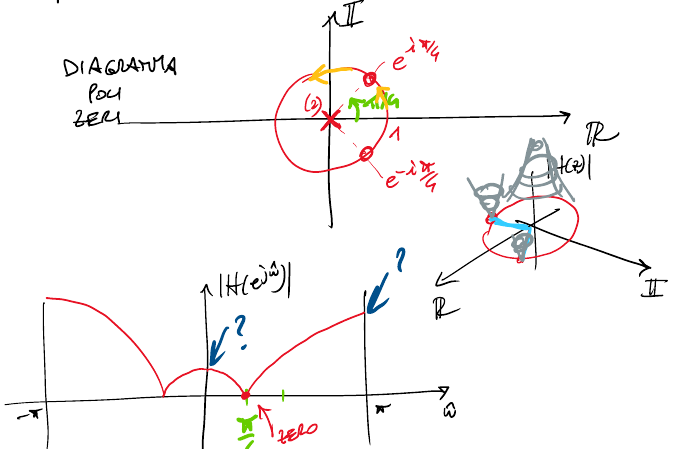
\includegraphics[scale=0.7]{immagini/lez28/es4v2.jpg}
\end{figure}

Quello che faccio e' disegnare inizialmente il diagramma poli zeri, poi lo uso per fare il grafico del modulo percorrendo la circonferenza del cerchio unitario da 1 a $\pi$. Da questo esempio possiamo notare che quando ho uno zero che e' sul cerchio, nel grafico del modulo quei punti vanno a zero, quindi e' come se stessi tagliando quelle frequenza, nel nostro esempio quelle a $\frac{\pi}{4}$.

\section{Esercizio}
Facciamo un esercizio un po' piu' complicato, data la seguente funzione di trasferimento:

\[
    H(z) = \frac{1 - \sqrt{3}z^{-1} + z^{-2}}{1 - 0,9 \sqrt{3} z^{-1} + 0,81 z^{-2}} = \frac{Y(z)}{X(z)}
\]  

Vogliamo trovare l'equazione alle differenze che l'ha generata. Per farlo dobbiamo fare la trasformata z inversa di Y(z) e X(z):

\[\begin{split}
    &X(z)[1 - \sqrt{3}z^{-1} + z^{-2}] = Y(z)[1 - 0,9 \sqrt{3} z^{-1} + 0,81 z^{-2}]\\
    &X(z) - \sqrt{3}z^{-1}X(z) + X(z) + z^{-2} = Y(z) - 0,9 \sqrt{3}z^{-1} Y(z) + 0,81z^{-2}Y(z)\\
    &\mbox{Facciamo la trasformata inversa}\\
    &x[n] - \sqrt{3} x[n-1] + x[n-2] = y[n] - 0,9 \sqrt{3} y[n-1] + 0,81 y[n-2]\\
    &y[n] = 0,9 \sqrt{3}y[n-1] - 0,81 y[n-2] + x[n] - \sqrt{3} x[n-1] + x[n-2]
\end{split}\]

Ora vogliamo disegnare il diagramma poli-zeri, desumendo un grafico approssimativo della risposta in frequenza, e dire che filtro e'.

Il consiglio e' di considerare sempre i polinomi con esponenti negativi, ma quando dobbiamo trovare i poli e gli zeri di portarli in positivo, per farlo in questo caso raccogliamo la potenza negativa maggiore sia al numeratore che al denominatore:

\[\begin{split}
    H(z) &= \frac{1 - \sqrt{3}z^{-1} + z^{-2}}{1 - 0,9 \sqrt{3} z^{-1} + 0,81 z^{-2}}\\
    &= \frac{z^{-2}(z^2 - \sqrt{3}z + 1)}{z^{-2}(z^2 - 0,9 \sqrt{3}z + 0,81)}
\end{split}\]

ora calcoliamo gli ZERI, portandoli in forma polare:
\[
    Z_{1,2} = \frac{\sqrt{3} \pm \sqrt{3-4}}{2} = \frac{\sqrt{3}}{2} \pm i\frac{1}{2} = e^{\pm i \frac{\pi}{3}}
\]

e i POLI, portandoli in forma polare:
\[
    P_{1,2} = \frac{0,9\sqrt{3}\pm \sqrt{0,81 \cdot 3 - 0,81 \cdot 4}}{2} = \frac{0,9 \sqrt{3} \pm 0,9 i}{2} = 0,9 (\frac{\sqrt{3}}{2} + \frac{1}{2}i) = e^{i \frac{\pi}{3}}
\]
\newpage

Ora riportiamo i poli e gli zeri nel grafico poli-zeri e come fatto in precedenza percorrendo il cerchio unitario disegniamo il grafico del modulo della risposta in frequenza.

\begin{figure}[ht!]
    \centering
    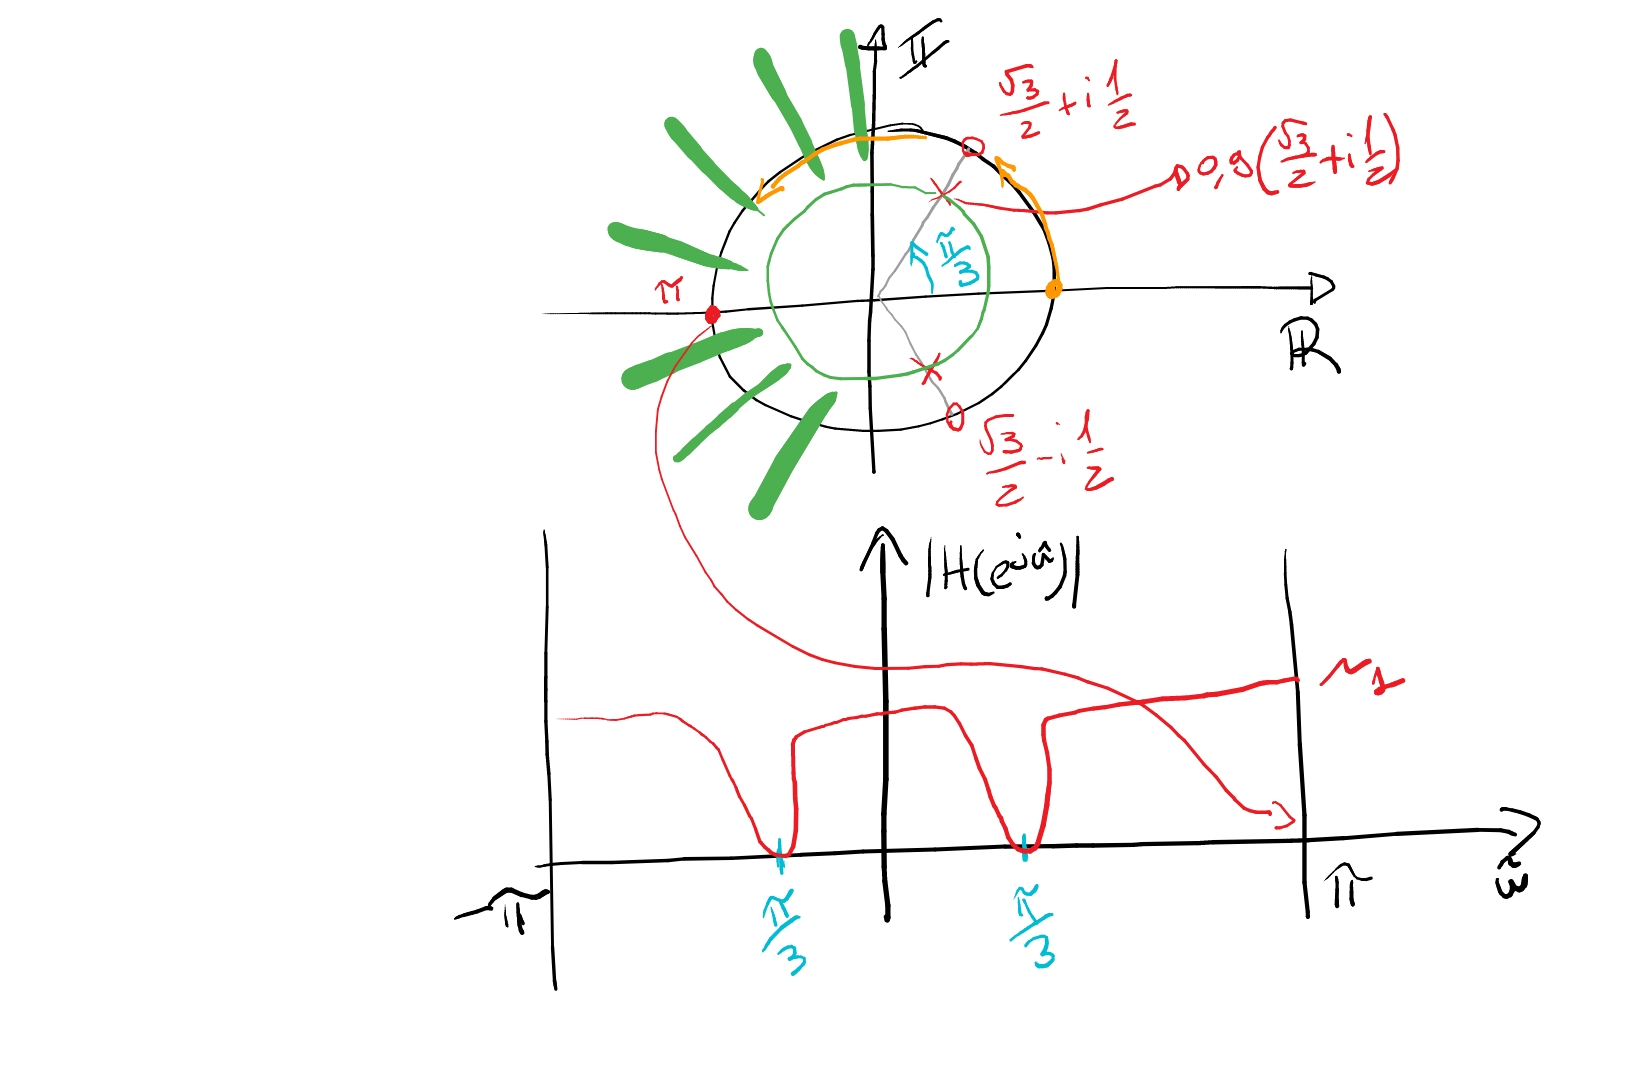
\includegraphics[scale=0.3]{immagini/lez29/graficoEs.jpg}
\end{figure}

\[
    z = e^{j \hat{\omega}} \in ROC \leftarrow X(z) = \frac{1 - \sqrt{3} e^{j\hat{\omega}} + e^{-j\hat{\omega}2}}{1 - 0,9 \sqrt{3} e^{-j\hat{\omega}} + 0,81 e^{-j 2 \hat{\omega}}} = H(e^{j\hat{\omega}})
\]

Una cosa da notare di questo esercizio e' che i poli o gli zeri posti all'origine degli assi non fanno niente, quindi possiamo non considerarli.
Questo filtro si chiama blocca banda.

\section{Esercizio}
Data la seguente funzione di trasferimento:

\[
    H(z) = \frac{1}{1 - 2 z^{-1}} + \frac{1}{1 - \frac{1}{3} z^{-1}}
\]

Ci viene detto che la ROC e' $\frac{1}{3} < |z| < 2$, vogliamo trovare la risposta in frequenza $h[n]$.

Per farlo dobbiamo applicare la trasformate z inversa, ma prima disegniamo il grafico poli-zeri per capire se il sistema e' causale o anticausale e capire che trasformata nota dobbiamo usare.

Gli zeri non li posso calcolare (o meglio dovrei fare il denominatore comune e trovare i numeratori), sappiamo pero' che i poli sono quelli che annullano i due denominatori,
quindi per il primo denominatore:

\[\begin{split}
    1 -2z^{-1} = 0 \\
    z^{-1} = \frac{1}{2}\\
    z = 2
\end{split}\]

per il secondo:
\[\begin{split}
    1 - \frac{1}{3} z^{-1} = 0\\
    z^{-1} = 3 \\
    z = \frac{1}{3}
\end{split}\]

Notiamo che i poli di polinomi di questo tipo sono sempre i numeri che moltiplicano la z.

\begin{figure}[ht!]
    \centering
    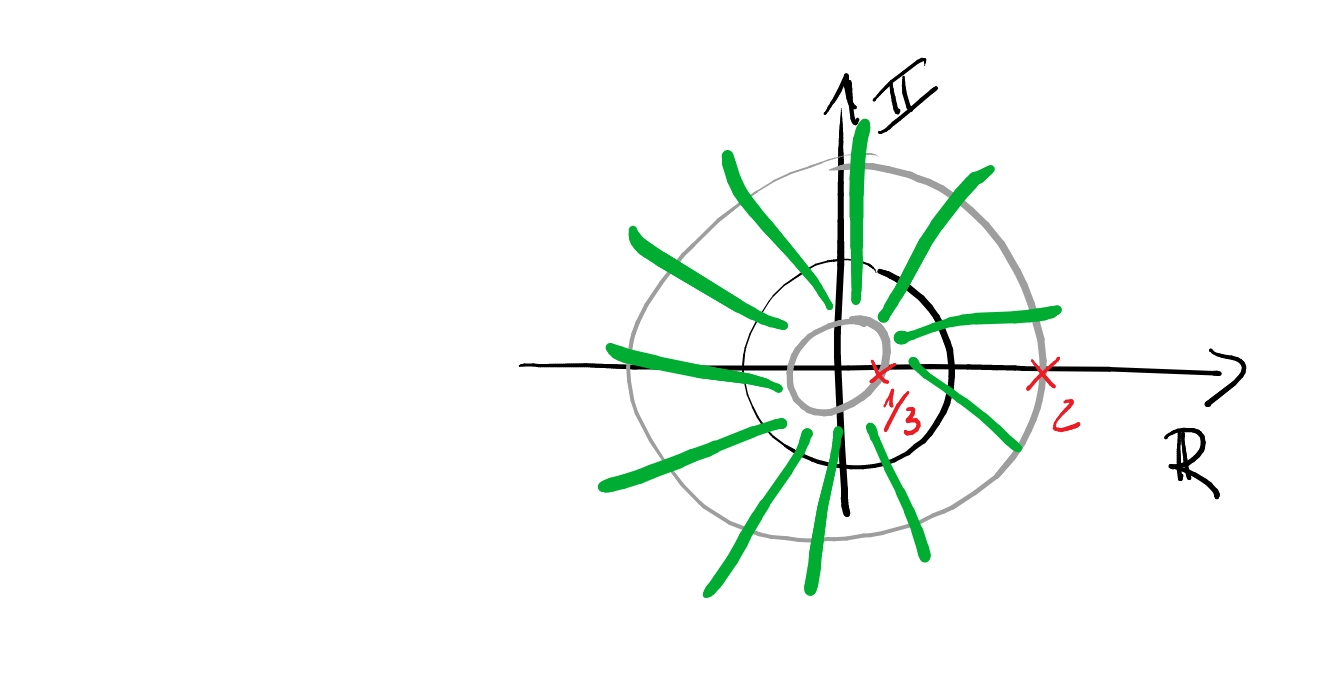
\includegraphics[scale=0.2]{immagini/lez29/poliZeriEsercizio.jpg}
\end{figure}

Quindi da questo grafico capiamo che per il primo polinomio dobbiamo usare il gradino anticausale, perche' la ROC e' minore di 2, quindi va verso l'interno. Al contrario per il secondo polinomio dobbiamo usare il gradino causale, perche' la ROC va da $\frac{1}{3}$ verso l'esterno.

\[\begin{split}
    h[n] &= Z^{-1} \{\frac{1}{1 - 2z^{-1}}\} + Z^{-1} \{\frac{1}{1 - \frac{1}{3} z^{-1}}\} \\
    h[n] &= -2^n u[-n-1] + (\frac{1}{3})^n u[n]
\end{split}\]

\section{All zeros, All poles}

Troviamo ora un collegamento tra filtri FIR, IIR e la loro quantita' di poli e zeri.

\begin{figure}[ht!]
    \centering
    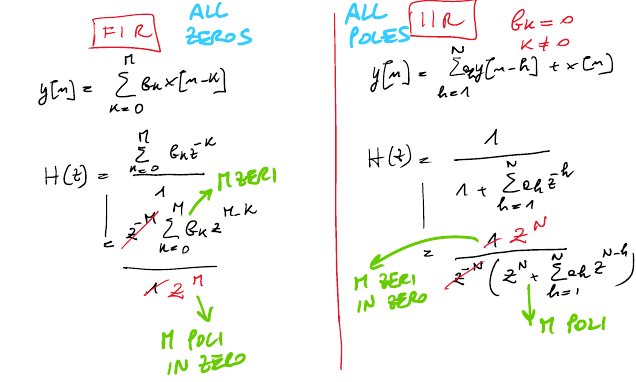
\includegraphics[scale=0.7]{immagini/lez29/allZeroAllPoles.jpg}
\end{figure}

Notiamo che i filtri FIR hanno M zeri e 0 poli, o meglio hanno M poli tutti in zero che come abbiamo visto in precedenza non contano. Viceversa i filtri IIR hanno M poli e M zeri tutti in zero (quindi non contano).

\section{Esempio}
Vediamo un esercizio che ci permettera' di introdurre una tecnica per calcolare la trasformata z inversa, la tecnica dei residui.

Partiamo da un equazione alle differenze causale:

\[
    y[n] = a_1 y[n-1] + b_0 x[n]
\]

Vogliamo ora calcolare l'uscita di questo sistema $y[n]$ se mettiamo in input:

\[
    x[n] = u[n]
\]

Quello che avremmo dovuto fare prima della trasformata Z era calcolare la convoluzione tra il sistema ed il segnale in input. 
Ma ora possiamo calcolare la funzione di trasferimento del sistema, la trasformata z del segnale e fare la moltiplicazione (propritea' della convoluzione) tra le due trasformate, successivamente fare la trasformata inversa del risultato trovando cosi' $y[n]$.

Quindi inizialmente calcoliamo la funzione di trasferimento $H(z)$ dell'equaazione alle differenze:

\[\begin{split}
    y[n] = a_1 y[n-1] + b_0 x[n]\\
    Y(z) = a_1 Y(z) z^{-1} + b X(z)\\
    Y(z) \{1 - a_1 z^{-1}\} = bX(z)\\
    \frac{y(z)}{X(z)} = \frac{b}{1 - a_1 z^{-1}} = H(z)
\end{split}\]

Della funzione di trasferimento possiamo dire che la ROC e' $|z| > |a|$, perche' sapevamo che il sistema che l'ha generata e' causale, inoltre esiste un solo polo che e' $a_1$.

Ora troviamo la trasformata z del segnale in input:

\[
    x[n] = u[n] \leftarrow \frac{1}{1 - z^{-1}} = X(z)
\]

Dato che e' un esponenziale causale (gradino causale) la ROC e' $|z| > 1$.

Ora facciamo la moltiplicazione tra le due trasformate che abbiamo trovato:

\[
    Y(z) = H(z) \cdot X(z) = \frac{b}{1 - a_1 z^{-1}} \cdot \frac{1}{1 - z^{-1}}
\]

Per trovare la ROC dobbiamo trovare qual'e' la condizione piu' stringente tra le ROC di ogni trasformata. Il problema diceva anche che $a_1 < 1$, quindi la condizione piu' stringente tra le due ROC e' $|z| > 1$. Inoltre abbiamo due poli, uno in $p_1 = 1$ e l'altro in $p_2 = a_1$.
Tracciamo il grafico poli-zeri:

\begin{figure}[ht!]
    \centering
    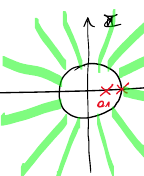
\includegraphics[scale=0.7]{immagini/lez29/poliZeroEs.jpg}
\end{figure}

Ora per trovare $Y(z)$ abbiamo due strategie, possiamo portare a denominatore comune le due frazioni e cercare in numeratori corretti:

\[\begin{split}
    Y(z) = \frac{b}{(1 - a_1 z^{-1})(1 - z^{-1})} = \frac{B_1}{(1 - a_1 z{-1}} + \frac{B_2}{(1 - z^{-1})}
\end{split}\]

Devo trovare i valori di $B_1$ e $B_2$, per farlo basta risolvere questo sistema:

\[\begin{split}
    &\begin{cases}
    B_1 + B_2 = b \\
    -B_1 - a_1B_2 = 0
    \end{cases}\\
    &B_2 - a_1B_2 = b\\
    &B_2 = \frac{b}{1 - a_1}\\
    &B_1 = b - B_2 = \frac{\cancel{b} -b a_1 \cancel{-b}}{1 - a_1}
\end{split}\]

da cui:

\[\begin{split}
    &\frac{B_1(1 - z^{-1}) + B_2(1-a_1 z^{-1})}{(1 - a_1 z^{-1})(1 - z^{-1})}\\
    &\frac{b}{1-a_1} \cdot \frac{1}{1-z^{-1}} - \frac{ba_1}{1 - a_1} \cdot \frac{1}{1 - a_1 z^{-1}}
\end{split}\]

e dato che il sistema e' causale otteniamo:

\[
    y[n] = \frac{b}{1 - a_1} u[n] - \frac{b a_1}{1 - a_1} a_1^n u[n]
\]

Oppure potevamo usare la TECNICA DEI RESIDUI, ma prima di utilizzarla dobbiamo fare 3 verifiche (altrimenti lasciamo stare):
\begin{enumerate}
    \item Il polinomio deve essere espresso in potenze negative $z^{-k}$
    \item I poli sono singoli, hanno molteplicita' 1 (non devono esserci due poli coincidenti in un punto solo)
\end{enumerate}

Quello che dobbiamo fare per trovare $B_1$ e $B_2$ e' moltiplicare la frazione per un fattore che cancella il polo (opposto del fattore che genera il polo), quindi:

\[\begin{split}
    B_1 &= [Y(z) \cdot(1 - p_1z^{-1})] = [\frac{b}{\cancel{(1 - a_1 z^{-1})}(1 - z^{-1})} \cdot \cancel{(1 - a_1 z^{-1})}] = \frac{b}{1 - a^{-1}} \\
    B_2 &= [Y(z) \cdot(1 - p_1z^{-1})] = [\frac{b}{(1 - a_1 z^{-1}) \cancel{(1 - z^{-1})}} \cdot \cancel{(1 - z^{-1})}] = \frac{b}{1 - a_1} \\
\end{split}\]

\section{Metodo dei residui}
Formalizziamo meglio il metodo dei residui che abbiamo appena visto.
Partiamo da una funzione di trasferimento, che come abbiamo gia' visto e' una funzione razionale fratta, per cui sappiamo che il numeratore e' un polinomio espresso in potenze negative di z, mentre il denominatore lo definiamo come una produttoria di poli della funzione di trasferimento. Il metodo dei residui ci serve per trovare la risposta all'impulso del sistema partendo dalla funzione di trasferimento.

\[\begin{split}
    H(z) &= \frac{N(z^{-1})}{\prod_{h=1}^{N} R_h \cdot \frac{1}{1 - p_h z^{-1}}}
\end{split}\]

Quello che facciamo quindi nel metodo dei residui e' trasformare la produttoria in una sommatoria in cui moltiplichiamo la funzione di trasferimento per un RESIDUO che mi serve per annullare lo zero della funzione.

Prima di applicare questa tecnica devo fare delle verifiche:
\begin{enumerate}
    \item Assicurarsi che i polinomi siano espressi in $z^{-1}$
    \item Assicurarsi che i poli siano semplici, ovvero che non abbiamo molteplicita' diversa da 1.
    \item Se il grado del numeratore e' minore del grado del denominatore. Se non lo fosse bisogna fare la divisione tra polinomi per abbassare i gradi dei polinomi.
\end{enumerate}

\[
R_h = [H(z)(1 - p_h z^{-1})]
\]

\section{Stabilita' di un filtro LTI}

Cosa intendiamo con stabilita' di un sistema.
Parliamo di stabilita' B.I.B.O (Bounded Input Bounded Output), che semplicemente ci dice che se in un sistema LTI mettiamo in input un segnale finito ci aspettiamo in output un segnale finito.

\begin{figure}[ht!]
    \centering
    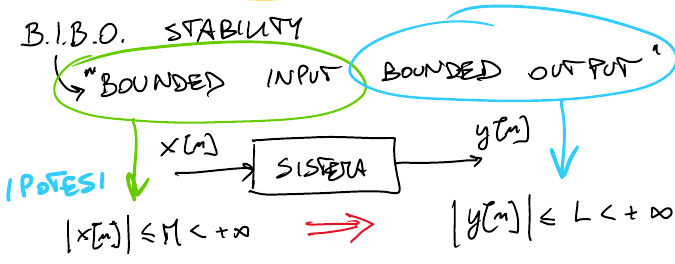
\includegraphics[scale=0.7]{immagini/lez30/BIBO.jpg}
\end{figure}

Un esempio semplice di una situazione che viola questa stabilita' e' ad esempio una cantante che fa scoppiare i bicchieri con la voce. La voce e' un input limitato che entrando in un sistema, il bicchiere, produce un output illimitato che fa scoppiare i bicchieri.
Un esempio piu' vicino all'elaborazione dei segnali e' quando un segnale satura e fischia.

\subsection{Teorema 1}
Dato un sistema LTI, condizione necessaria e sufficiente per la BIBO stabilita' e' che la risposta all'impulso sia assolutamente sommabile:

\[
    \sum_{n = -\infty}^{+\infty} |h[n]| < + \infty
\]

Dimostriamo la parte sufficiente:

Se LTI $ \sum_{n = -\infty}^{+\infty} |h[n]| < + \infty$ allora il sistema LTI e' stabile

\[\begin{split}
    y[n] &= x[n] * h[n] = \sum_{k = -\infty}^{+\infty} h[k] x[n-k]\\
    |y[n]| &= |\sum_{k = -\infty}^{+\infty} h[k] x[n-k]| \le \sum_{k = -\infty}^{+\infty} |h[k] x[n-k]| \\
    &= \sum_{k = -\infty}^{+\infty} |h[k]| |x[n-k]| \le \sum_{k = -\infty}^{+\infty} |h[k]| \cdot M \\
    &= M \sum_{k = -\infty}^{+\infty} h[k] = M \Tilde{h}\\
    |y[n]| &\le M \Tilde{h} < +\infty
\end{split}\]



\end{document}
